%----------------------------------------------------------------------------------------
%	PACKAGES AND OTHER DOCUMENT CONFIGURATIONS
%----------------------------------------------------------------------------------------

\documentclass[
11pt, % The default document font size, options: 10pt, 11pt, 12pt
%oneside, % Two side (alternating margins) for binding by default, uncomment to switch to one side
english, % ngerman for German
onehalfspacing, % Single line spacing, alternatives: onehalfspacing or doublespacing
%draft, % Uncomment to enable draft mode (no pictures, no links, overfull hboxes indicated)
%nolistspacing, % If the document is onehalfspacing or doublespacing, uncomment this to set spacing in lists to single
liststotoc, % Uncomment to add the list of figures/tables/etc to the table of contents
%toctotoc, % Uncomment to add the main table of contents to the table of contents
%parskip, % Uncomment to add space between paragraphs
%nohyperref, % Uncomment to not load the hyperref package
headsepline, % Uncomment to get a line under the header
%chapterinoneline, % Uncomment to place the chapter title next to the number on one line
%consistentlayout, % Uncomment to change the layout of the declaration, abstract and acknowledgements pages to match the default layout
]{MastersDoctoralThesis} % The class file specifying the document structure

\usepackage[utf8]{inputenc}
\usepackage[T1]{fontenc} 
\usepackage{graphicx}
\usepackage{amsmath}
\usepackage{amsfonts}
\usepackage[justification=centering,font=scriptsize]{subfig}
\usepackage[font=small,labelfont=bf,justification=justified,format=plain]{caption}
\usepackage{multirow}
\usepackage{lettrine}
\usepackage{pdfpages}
\usepackage{comment}
\usepackage{adjustbox}

\usepackage[autostyle=true]{csquotes} % Required to generate language-dependent quotes in the bibliography
\usepackage[backend=bibtex,style=alphabetic,natbib=true,maxbibnames=99,doi=false,isbn=false,url=false,eprint=false]{biblatex}

%\usepackage[square,numbers,sectionbib]{natbib}
%\usepackage{chapterbib}


\DeclareMathOperator*{\argmax}{arg\,max}
\DeclareMathOperator*{\argmin}{arg\,min}

\newcommand{\SK}[1]{\textcolor{blue}{#1}}
\newcommand{\PA}[1]{\textcolor{red}{#1}}

\addbibresource{ref.bib}

%----------------------------------------------------------------------------------------
%	MARGIN SETTINGS
%----------------------------------------------------------------------------------------

\geometry{
	paper=a4paper, % Change to letterpaper for US letter
	inner=2.5cm, % Inner margin
	outer=3.8cm, % Outer margin
	bindingoffset=.5cm, % Binding offset
	top=1.5cm, % Top margin
	bottom=1.5cm, % Bottom margin
	%showframe, % Uncomment to show how the type block is set on the page
}

%----------------------------------------------------------------------------------------
%	THESIS INFORMATION
%----------------------------------------------------------------------------------------

\thesistitle{Deep learning for speaker counting and localization wwith Ambisonics signals} % Your thesis title, this is used in the title and abstract, print it elsewhere with \ttitle
\supervisor{Pr. Laurent \textsc{Girin}} % Your supervisor's name, this is used in the title page, print it elsewhere with \supname
\examiner{} % Your examiner's name, this is not currently used anywhere in the template, print it elsewhere with \examname
\degree{Doctor of Philosophy} % Your degree name, this is used in the title page and abstract, print it elsewhere with \degreename
\author{Pierre-Amaury \textsc{Grumiaux}} % Your name, this is used in the title page and abstract, print it elsewhere with \authorname


\subject{Biological Sciences} % Your subject area, this is not currently used anywhere in the template, print it elsewhere with \subjectname
\keywords{Sound source localization, source counting, deep learning, neural networks, Ambisonics} % Keywords for your thesis, this is not currently used anywhere in the template, print it elsewhere with \keywordnames
\university{\href{http://www.university.com}{University Name}} % Your university's name and URL, this is used in the title page and abstract, print it elsewhere with \univname
\department{\href{http://department.university.com}{Department or School Name}} % Your department's name and URL, this is used in the title page and abstract, print it elsewhere with \deptname
\group{\href{http://researchgroup.university.com}{Research Group Name}} % Your research group's name and URL, this is used in the title page, print it elsewhere with \groupname
\faculty{\href{http://faculty.university.com}{Faculty Name}} % Your faculty's name and URL, this is used in the title page and abstract, print it elsewhere with \facname

\AtBeginDocument{
\hypersetup{pdftitle=\ttitle} % Set the PDF's title to your title
\hypersetup{pdfauthor=\authorname} % Set the PDF's author to your name
\hypersetup{pdfkeywords=\keywordnames} % Set the PDF's keywords to your keywords
}

\begin{document}

\frontmatter % Use roman page numbering style (i, ii, iii, iv...) for the pre-content pages

\pagestyle{plain} % Default to the plain heading style until the thesis style is called for the body content

%----------------------------------------------------------------------------------------
%	GRENOBLE EEATS COVER PAGE
%----------------------------------------------------------------------------------------

%% ERR: Deux fois "Examinateur" pour Roland Badeau
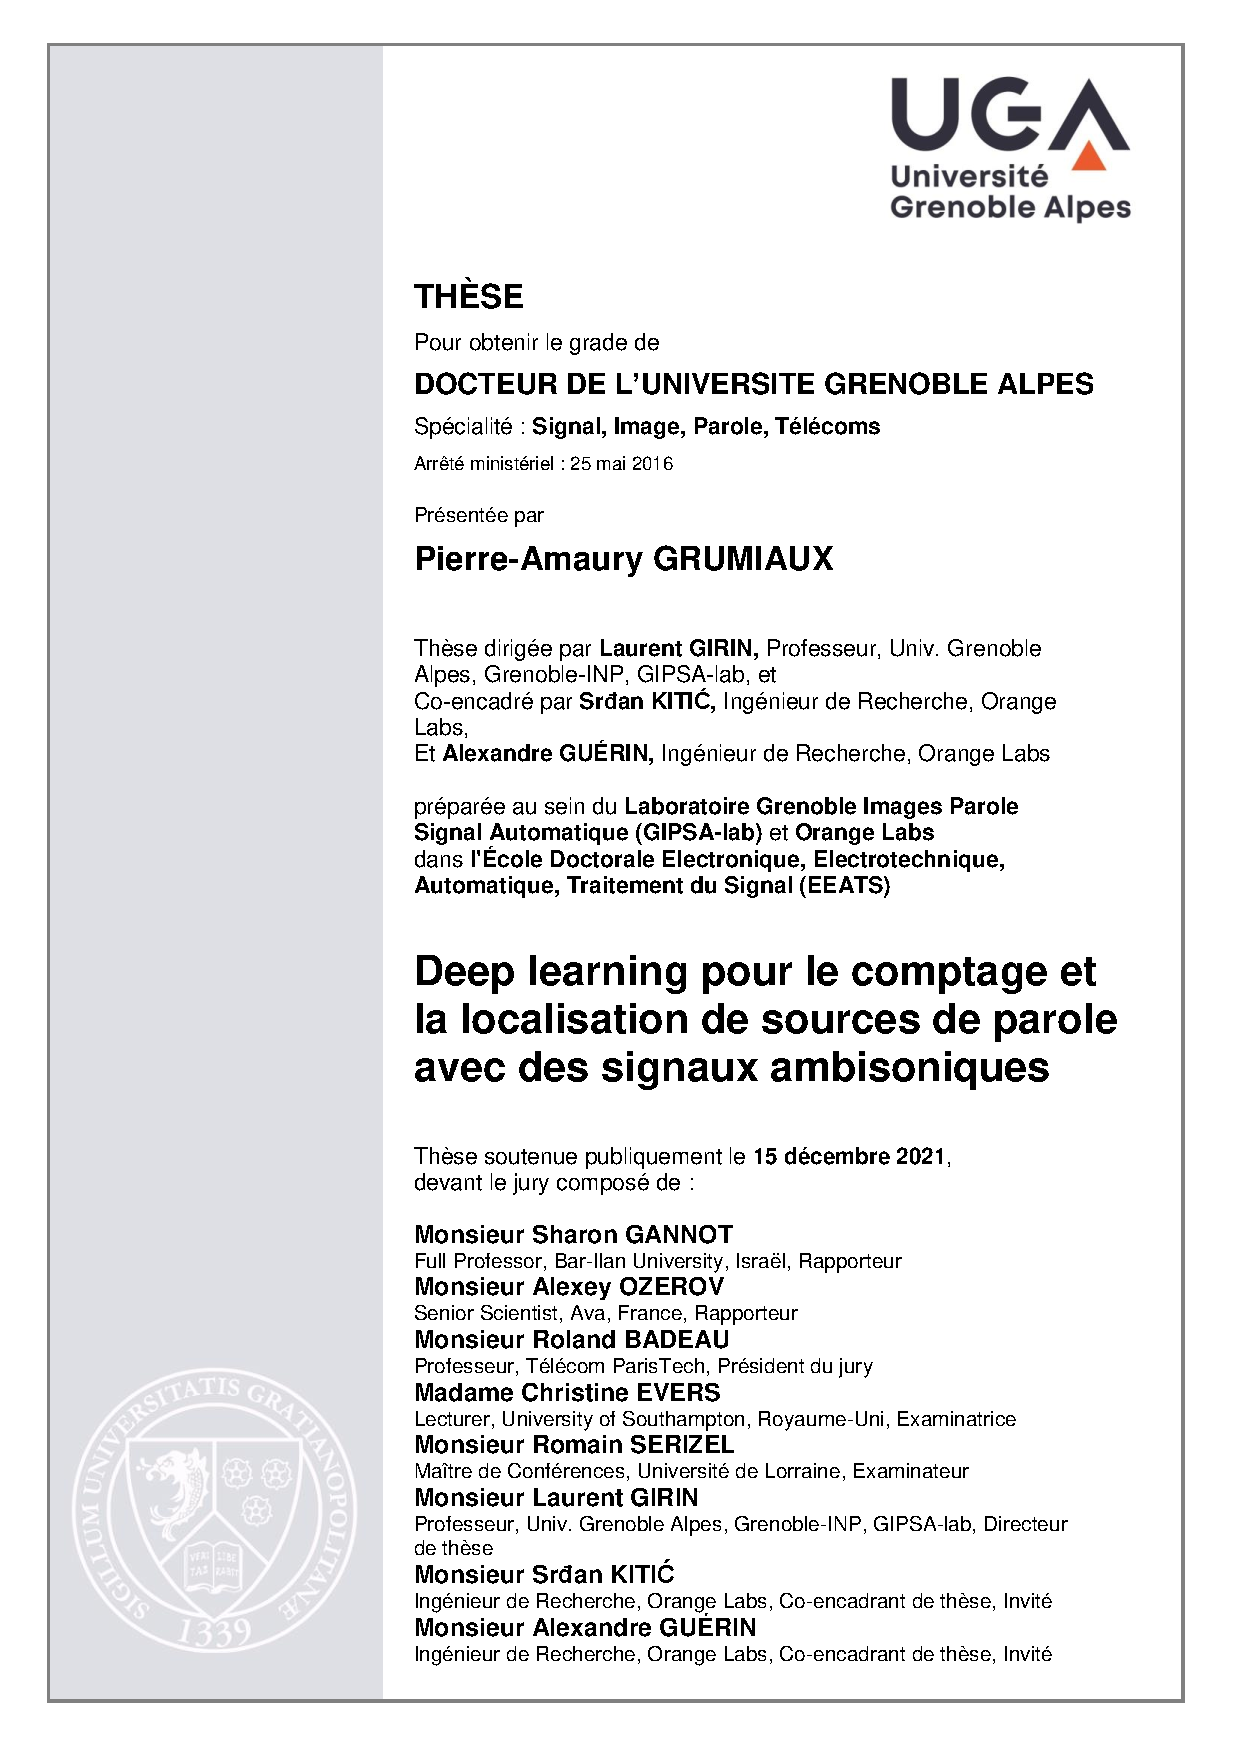
\includepdf[pages=-]{cover.pdf}

%----------------------------------------------------------------------------------------
%	TITLE PAGE
%----------------------------------------------------------------------------------------
\begin{comment}
\begin{titlepage}
\begin{center}

\vspace*{.06\textheight}
{\scshape\LARGE \univname\par}\vspace{1.5cm} % University name
\textsc{\Large Doctoral Thesis}\\[0.5cm] % Thesis type

\HRule \\[0.4cm] % Horizontal line
{\huge \bfseries \ttitle\par}\vspace{0.4cm} % Thesis title
\HRule \\[1.5cm] % Horizontal line
 
\begin{minipage}[t]{0.4\textwidth}
\begin{flushleft} \large
\emph{Author:}\\
\href{http://www.johnsmith.com}{\authorname} % Author name - remove the \href bracket to remove the link
\end{flushleft}
\end{minipage}
\begin{minipage}[t]{0.4\textwidth}
\begin{flushright} \large
\emph{Supervisor:} \\
\href{http://www.jamessmith.com}{\supname} % Supervisor name - remove the \href bracket to remove the link  
\end{flushright}
\end{minipage}\\[3cm]
 
\vfill

\large \textit{A thesis submitted in fulfillment of the requirements\\ for the degree of \degreename}\\[0.3cm] % University requirement text
\textit{in the}\\[0.4cm]
\groupname\\\deptname\\[2cm] % Research group name and department name
 
\vfill

{\large \today}\\[4cm] % Date
%\includegraphics{Logo} % University/department logo - uncomment to place it
 
\vfill
\end{center}
\end{titlepage}
\end{comment}

%-------------------------------------------------------------------------------
%	PREAMBLE PAGES
%-------------------------------------------------------------------------------

\begin{abstract}
\addtocontents{toc}{\vspace{-0.5cm}}
\addchaptertocentry{\abstractname}

Sound source localization (SSL) is a subtask of audio scene analysis that has challenged researchers for more than four decades. Traditional methods (e.g., MUSIC or GCC-PHAT) impose strong assumptions on the sound propagation, number of active sources and/or signal content, which makes them vulnerable to adverse acoustic phenomena, such as reverberation and noise. Recently, data-driven models -- and particularly deep neural networks – have shown increased robustness in noisy and reverberant environments. However, their performance is still seriously degraded in the presence of multiple sound sources, especially when their number is unknown. Moreover, source detection and localization in real-life use-cases, where the latency is an important criterion, is still an open research problem. 
 
In this thesis, we focus on speaker detection and localisation in office/domestic indoor environments, using multichannel Ambisonics recordings, with the emphasis on low-latency performance. First, we propose to use deep neural networks (DNNs) to estimate the number of speakers (NoS) in a multichannel mixture. We propose a model that is capable to count up to five speakers, with a relatively high accuracy, at the short-term-frame resolution. We also provide a performance analysis of this model depending on several hyperparameters, which gives interesting insights on its behavior. Second, we explore the capabilities of a multichannel audio signal representation called time-domain velocity vector (TDVV), akin to relative impulse response in the present spherical harmonics domain, as a novel type of input features of DNNs for detection/localization tasks. Next, we address multi-speaker localization, by first improving upon a state-of-the-art convolutional recurrent neural network (CRNN) with a substantial gain in accuracy. We also examine the potential of self-attention-based neural networks for multi-speaker localization, as these models are known to be suitable for other audio processing tasks due to their capability to capture both short- and long-term dependencies in the input signal. Furthermore, we investigate the use of the estimated NoS, provided by our speaker counting neural network, to improve our speaker localization CRNN. We show experimentally that using the estimated NoS leads to more robust multi-speaker localization than the classical threshold-based direction of arrival (DoA) estimation. Moreover, we show the interest of injecting the NoS information as an additional input feature for the localization neural network. Finally, we explore multi-task neural architectures to estimate both the NoS and speaker DoAs at the same time.

\end{abstract}
\begin{resume}
\addchaptertocentry{Résumé}

La localisation de sources sonores est une sous-tâche de l'analyse de scènes sonores qui a défié les chercheurs pendant plus de quatre décennies. Les méthodes traditionnelles (e.g., MUSIC ou GCC-PHAT) imposent des hypothèses fortes sur la propagation du son, le nombre de sources actives et/ou le contenu du signal, ce qui les rend vulnérables à des phénomènes acoustiques adverses tels que la réverbération ou le bruit. Récemment, les méthodes basées sur les données -- et particulièrement les réseaux de neurones profonds – ont montré une plus grande robustesse dans les environnements réverbérants et bruités. Cependant, leur performance est toujours sensiblement dégradée en présence de plusieurs sources sonores, notamment quand leur nombre est inconnu. De plus, la détection et la localisation de sources pour des usages pratiques, où la latence joue un rôle important, est toujours un sujet de recherche ouvert.

Dans cette thèse, nous nous intéressons à la détection et à la localisation de locuteurs dans des environnements domestiques, en utilisant des enregistrements ambisoniques multicanaux, avec un accent sur une performance à basse latence. Tout d'abord, nous proposons d'utiliser des réseaux de neurones profonds (DNN, pour deep neural network) pour estimer le nombre de locuteurs (NoS, number of sources) dans un mélange multicanal. Notre modèle est capable de compter jusqu'à cinq locuteurs, avec une précision relativement grande, pour une résolution à la trame. Nous proposons également une analyse de la performance du modèle en fonction de certains hyperparamètres, ce qui fournit des informations intéressantes sur son comportement. Ensuite, nous explorons les capacités d'une représentation d'un signal audio multicanal appelée vecteur vélocité dans le domaine temporel (TDVV, time-domain velocity vector), qui est analogue à la réponse impulsionnelle relative dans le domaine des harmoniques sphériques, en tant que nouvelle représentation d'entrée de DNNs pour la localisation/détection. Par la suite, nous nous penchons sur la localisation de plusieurs locuteurs en commençant par améliorer un réseau de neurones convolutif et récurrent (CRNN, convolutional recurrent neural network) de l'état de l'art avec un gain important en précision. Puis nous examinons le potentiel des mécanismes de self-attention pour la localisation de plusieurs locuteurs, alors que ces modèles sont connus pour être adaptés à d'autres tâches de traitement audio étant donnée leur capacité à capter les dépendances à court et long terme dans le signal d'entrée. En outre, nous investiguons l'utilisation du NoS estimé, fourni par notre réseau de neurones de comptage, pour améliorer le CRNN de localisation. Nous montrons expérimentalement qu'utiliser le NoS estimé donne plus de robustesse à la localisation multi-locuteur que la méthode de seuillage classiquement utilisée dans l'estimation de direction d'arrivée (DoA, direction of arrival). De plus, nous montrons l'intérêt d'injecter l'information du NoS en tant qu'entrée additionnelle pour le réseau de neurones de localisation. Finalement, nous explorons les architectures neuronales multi-tâches pour estimer le NoS et la DoA des locuteurs dans le même temps.
\end{resume}
\begin{acknowledgements}
\addchaptertocentry{\acknowledgementname}

First, I would like to thank my academic supervisor Laurent Girin. I have really appreciated all your advice and recommendations which I believe have taught me precious principles on the research work. Although the distance were not our ally, you always took your time to attend the meetings, answer my questions and review my works. I also thank Sr\dj{}an Kiti\'{c} and Alexandre Gu\'{e}rin, my industry supervisors, with whom I spent most of my time when we were at the office. I think you have guided on the right path during this thesis, by suggesting me a lot of food for thought and being very helpful when I had some doubts over technical considerations. With you three, I have learned a lot, on the technical, the methodological and ethical aspects, so again, thank you. 

I also thank my other colleagues at Orange Labs, with whom I spent more or less time at the office: Arnaud, Cl\'{e}ment, Gil, Gr\'{e}gory, Laur\'{e}line, Marc, Michel, Thomas. I spent many pleasing moments, around a coffee, a drink or at the restaurant. Thank you to my colleagues at Lannion as well, I greatly enjoyed the few times we met, with a special thanks to J\'{e}r\^{o}me who provided me with his expertise during part of my experiments. Also, thanks to Prerak, J\'{e}r\'{e}mi and Th\'{e}odoric who delved into considerations I did not have time to explore during my thesis.

This thesis has been evaluated by a jury of which I would like to thank all the members: Sharon Gannot et Alexey Ozerov who took the time to review this manuscript, and Roland Badeau, Christine Evers and Romain Serizel for being present at my PhD defense. Special thanks for the latter, as well as Nancy Bertin, who took an interest in my thesis from the beginning by being a member of the thesis follow-up committee.

Thanks to the members of the GIPSA-lab, my academic laboratory, whom I had the chance to met for only a couple of weeks during the first year of my PhD. I have good memories of our few discussions.

Finally, thanks to my family and friends, for their support during these three years, even though most of you were without a clue of what I was doing. Thanks a lot to Manon, with whom I have spent most of my everyday life and who supported me throughout this period. You helped me escape from my thesis work from time to time, notably with amazing trips around Bretagne.

\emph{P.S.}: Special thanks to Covid-19, without whom I would have not spent so many hours on the piano or producing music instead of playing volley-ball.

\end{acknowledgements}
\cleardoublepage

\vspace*{0.2\textheight}

\noindent\enquote{\itshape The composer of the past has been like the chemist or alchemist of ancient time, who could use in his combinations some few compound bodies only. The composer of the future will have in the sinusoidal vibrations of electrical music those pure elements out of which all tone-compounds can be built; not merely the known and approved tones of the orchestra, but many shades and nuances heretofore unattainable.}\bigbreak

\hfill Thaddeus Cahill, 1907

%-------------------------------------------------------------------------------
%	LIST OF CONTENTS/FIGURES/TABLES
%-------------------------------------------------------------------------------
\setcounter{tocdepth}{2}
\tableofcontents
\listoffigures
\listoftables
%-------------------------------------------------------------------------------
%	ACRONYMS AND NOTATIONS
%-------------------------------------------------------------------------------

\begin{abbreviations}{ll}

\textbf{ANN}    & \textbf{A}rtificial \textbf{N}eural \textbf{N}etwork\\
\textbf{ASR}    & \textbf{A}utomatic \textbf{S}peech \textbf{R}ecognition\\
\textbf{BiLSTM} & \textbf{Bi}directional \textbf{L}ong \textbf{S}hort-\textbf{T}erm \textbf{M}emory\\
\textbf{BPTT}   & \textbf{B}ack\textbf{P}ropagation \textbf{T}hrough \textbf{T}ime\\
\textbf{CMH}    & \textbf{C}ross-\textbf{M}ulti-\textbf{H}ead\\
\textbf{CNN}    & \textbf{C}onvolutional \textbf{N}eural \textbf{N}etwork\\
\textbf{CRNN}   & \textbf{C}onvolutional \textbf{R}ecurrent \textbf{N}eural \textbf{N}etwork\\
\textbf{DAW}    & \textbf{D}igital \textbf{A}udio \textbf{W}orkstation\\
\textbf{DL}     & \textbf{D}eep \textbf{L}earning\\
\textbf{DoA}    & \textbf{D}irectional \textbf{o}f \textbf{A}rrival\\
\textbf{ESPRIT} & \textbf{E}stimation of \textbf{S}ignal \textbf{P}arameters via \textbf{R}otational \textbf{I}nvariance \textbf{T}echniques\\
\textbf{FDVV}   & \textbf{F}requency-\textbf{D}omain \textbf{V}elocity \textbf{V}ector\\
\textbf{FF}     & \textbf{F}eed\textbf{F}orward\\
\textbf{FOA}    & \textbf{F}irst-\textbf{O}rder \textbf{A}mbisonics\\
\textbf{GCC}    & \textbf{G}eneralized \textbf{C}ross-\textbf{C}orrelation\\
\textbf{GPU}    & \textbf{G}raphical \textbf{P}rocessing \textbf{U}nit\\
\textbf{GRU}    & \textbf{G}ated \textbf{R}ecurrent \textbf{U}nit\\
\textbf{HOA}    & \textbf{H}igher-\textbf{O}rder \textbf{A}mbisonics\\
\textbf{IFT}    & \textbf{I}nverse \textbf{F}ourier \textbf{T}ransform\\
\textbf{IPD}    & \textbf{I}nteraural \textbf{P}hase \textbf{D}ifference\\
\textbf{ISM}    & \textbf{I}mage-\textbf{S}ource \textbf{M}ethod\\
\textbf{LSTM}   & \textbf{L}ong \textbf{S}hort-\textbf{T}erm \textbf{M}emory\\
\textbf{MFCC}   & \textbf{M}el \textbf{F}requency \textbf{C}epstral \textbf{C}oefficients\\
\textbf{MH}     & \textbf{M}ulti-\textbf{H}ead\\
\textbf{MLP}    & \textbf{M}ulti\textbf{L}ayer \textbf{P}erceptron\\
\textbf{MSE}    & \textbf{M}ean \textbf{S}quared \textbf{E}rror\\ 
\textbf{MUSIC}  & \textbf{MU}ltiple \textbf{SI}gnal \textbf{C}lassification\\
\textbf{NLP}    & \textbf{N}atural \textbf{L}anguage \textbf{P}rocessing\\
\textbf{NoS}    & \textbf{N}umber \textbf{o}f \textbf{S}ources\\
\textbf{PHAT}   & \textbf{PHA}se \textbf{T}ransform\\
\textbf{PIV}    & \textbf{P}seudo\textbf{I}ntensity \textbf{V}ector\\
\textbf{ReLU}   & \textbf{Re}ctified \textbf{L}inear \textbf{U}nit\\
\textbf{RIR}    & \textbf{R}oom \textbf{I}mpulse \textbf{R}esponse\\
\textbf{RNN}    & \textbf{R}ecurrent \textbf{N}eural \textbf{N}etwork\\
\textbf{RTF}    & \textbf{R}elative \textbf{T}ransfer \textbf{F}unction\\
\textbf{RT60}   & \textbf{R}everberation \textbf{T}ime $\mathbf{60}$~dB\\
\textbf{SA}     & \textbf{S}elf-\textbf{A}ttention\\
\textbf{SCM}    & \textbf{S}patial \textbf{C}ovariance \textbf{M}atrix\\
\textbf{SHD}    & \textbf{S}pherical \textbf{H}armonics \textbf{D}ecomposition\\
\textbf{SIR}    & \textbf{S}ignal-to-\textbf{I}nterference \textbf{R}atio\\
\textbf{SNR}    & \textbf{S}ignal-to-\textbf{N}oise \textbf{R}atio\\
\textbf{SPL}    & \textbf{S}ound \textbf{P}ressure \textbf{L}evel\\
\textbf{SRP}    & \textbf{S}teered \textbf{R}esponse \textbf{P}ower\\
\textbf{SSL}    & \textbf{S}ound \textbf{S}ource \textbf{L}ocalization\\
\textbf{STFT}   & \textbf{S}hort-\textbf{T}erm \textbf{F}ourier \textbf{T}ransform\\
\textbf{TCN}    & \textbf{T}emporal \textbf{C}onvolutional \textbf{N}etwork\\
\textbf{TDoA}   & \textbf{T}ime-\textbf{D}ifference \textbf{o}f \textbf{A}rrival\\
\textbf{TDVV}   & \textbf{T}ime-\textbf{D}omain \textbf{V}elocity \textbf{V}ector\\
\textbf{TF}     & \textbf{T}ime-\textbf{F}requency\\
\textbf{VAD}    & \textbf{V}oice \textbf{A}ctivity \textbf{D}etection\\
\textbf{VR}     & \textbf{V}irtual \textbf{R}eality\\

\end{abbreviations}
\begin{symbols}{ll}

\textbf{Linear algebra}\\
$x$                 & scalar\\
$\mathbf{x}$        & vector\\
$\mathbf{X}$        & tensor\\
$\mathbf{x}^T$      & transpose of $\mathbf{x}$\\
$x^*$               & complex conjugate of $x$\\
$\mathfrak{R}(x)$   & real part of $x$\\
$\mathfrak{I}(x)$   & imaginary part of $x$\\
\addlinespace
\addlinespace

\textbf{Indexes}\\
$I$                 & number of microphones \\
$i$                 & microphone index\\
$J$                 & total number of sources\\
$\bar{J}$           & maximum number of sources\\
$J(t)$              & instantaneous number of sources\\
$j$                 & source index\\
$T$                 & number of frames\\
$t$                 & time or frame index\\
$\tau$              & alternative time index\\
$F$                 & number of frequency bins\\
$f$                 & frequency bin index\\
$\omega$            & angular frequency\\
\addlinespace
\addlinespace

\textbf{Geometry}\\
$\mathbf{r}_j$      & position of source $j$\\
$x_j$, $y_j$, $z_j$ & cartesian coordinates of source $j$\\
$r_j$               & distance of source $j$ from the array origin\\
$\theta_j$          & azimuth of source $j$\\
$\phi_j$            & elevation of source $j$\\
\addlinespace
\addlinespace

\textbf{Signal}\\
$\mathbf{x}$        & $I \times 1$ multi-channel input signal\\
$x_i$               & input signal recorded at microphone $i$\\
$c_{ij}$            & signal from source $j$ recorded at microphone $i$\\
$a_{ij}$            & room impulse response from source $j$ to microphone $i$\\
$n_i$               & noise signal recorded at microphone $i$\\
\addlinespace
\addlinespace

\textbf{Acoustics}\\
$p$                 & acoustic pressure \\
$c$                 & speed of sound \\
$Y_n^m$             & complex spherical harmonic at order $n$ and degree $m$\\
$\tilde{Y}_n^m$     & real spherical harmonic at order $n$ and degree $m$\\
$N$                 & Ambisonics order\\
$B_n^m$             & Ambisonics coefficient at order $n$ and degree $m$\\
$W$                 & Ambisonics coefficient $B_0^0$\\
$X$, $Y$, $Z$       & Ambisonics coefficients $B_1^1$, $B_1^{-1}$ and $B_1^0$, respectively\\
$\mathbf{I}$        & complex intensity or pseudointensity vector (at order 1)\\
$\mathbf{I}^N$      & complex pseudointensity vector at order $N$ \\
$\mathbf{I}_a$      & complex active intensity or pseudointensity vector\\
$\mathbf{I}_r$      & complex reactive intensity or pseudointensity vector\\
$\mathbf{V}(t)$     & time-domain velocity vector\\
$\mathbf{V}(f)$     & frequency-domain velocity vector\\
\addlinespace
\addlinespace

\textbf{Metrics}\\
$A_{ij}$            & Entry of the confusion matrix $\mathbf{A}$ for ground-truth NoS $i$ and predicted NoS $j$\\
$A(\tau)$           & Overall classification accuracy for predictions at frame $\tau$\\
$M_i$               & Mean absolute error for class $i$\\

\end{symbols}

%----------------------------------------------------------------------------------------
%	THESIS CONTENT - CHAPTERS
%----------------------------------------------------------------------------------------

\mainmatter % Begin numeric (1,2,3...) page numbering

\pagestyle{thesis} % Return the page headers back to the "thesis" style

\chapter{Introduction}
\label{chap:introduction}

%-----------------------------------------------
%  GENERAL CONTEXT
%-----------------------------------------------
\section{General context}

\subsection{Human hearing}

\lettrine{W}{e}, as humans, have been granted a couple of ears capable of reacting to surrounding sound and processing the vibrations through our brain. From even before our birth, we have learned to use them properly, and we have impressive capabilities of dealing with a complex sound environment.

Imagine yourself at a friend's party. Many guests are present, you are in the middle of a discussion with two friends, surrounded with other small groups of chatting people. A few meters from you, one of the guest performs an entertaining dub music DJ set, while someone is ringing at the door. A lot of audio information arrive at the same time to your ears. Yet, you are still able to understand what your two friends are debating, and you can handle the conversation, maybe at the cost of speaking louder. Also, you can shift your attention at any time by indiscreetly listening the next group's conversation, or enjoying the music coming from the DJ booth, while being aware that a new guest is arriving at the door. This phenomenon is called the \textit{cocktail party effect} \cite{arons_review_1992}. It refers to the brain's ability to let us focus on any sound stimulus among many other stimuli. In other words, the fact that all sounds are mixed together when incoming to our ears is not an obstacle for us to understand the surrounding sound space.

The cocktail party effect is partially due to our great ability for sound source localization. Because our ears do not receive the exact same sound signal at a given instant, the brain can sense small differences in intensity, spectral content and timing cues between the two signals in order to locate the sound sources \cite{bregman_auditory_1994}. Except if a sound source location is equidistant to both ears, the signals arrive time-shifted from each other and this time difference is a localization cue. The shapes of our head, torso and pinna cause diffraction which also helps to locate sound sources \cite{blauert_spatial_1997}. Consequently, all human beings perceive sound differently, and we have learned to hear based on the characteristics of the body parts around our ears. We are also capable of estimating the source distance based on the loss of amplitude and the ratio between the direct path and the reverberated part. Thus, our localization ability is greatly responsible for our capacity to extract meaningful information from a complex sound environment.

\subsection{What is sound ?}

Sound is a vibration travelling through a medium. It propagates, as a wave, in any medium allowing local oscillations: gases, fluids and solids. On Earth, silence almost does not exist. Any vibrating object, like flowers, tree leaves, fleas, fish, wind, icebergs, underwater volcanoes, loudspeaker, guitar string, emits a sound wave and acts as a sound source. The resulting vibration then freely travels through the surrounding medium, if no obstacle is encountered, at a speed $c$ depending on the medium properties (in the air, $c = \SI{343}{\meter\per\second}$ at $\SI{20}{\degreeCelsius}$). When a sound wave passes through a fixed point in space, local pressure and velocity vary in time, a little shifted from the equilibrium state. The changes are generally very small. On Earth, the average atmospheric pressure at the surface is around $100\,000$~Pa, while the just audible pressure deviation for human hearing is $0.00002$~Pa (corresponding to $0$~dB in sound pressure level, SPL), and the threshold of pain is between $20$ and $200$~Pa (corresponding to $120$-$140$~dB SPL). 

In such a vibrating phenomenon, frequency is defined as the number of vibrations per second, or \textit{Hertz} (Hz). In nature, most sound waves are propagating vibrations containing multiple frequencies, which characterize its  aspect, commonly referred as \textit{timbre}. For example, a guitar bass sound is mainly made of \textit{low} frequencies, whereas a singing bird mostly emits \textit{high} frequencies. We can describe a complex wave (\emph{i.e.}, containing many frequencies) in terms of a superposition of sinusoidal plane waves, each one containing only one frequency. As a sound source vibration evolves with time (for instance, it can attenuate), its frequency content also evolves. Thus, the time and frequency dimensions are two important characteristics of a sound wave.

When a sound wave encounters an obstacle, several phenomena can occur. \textit{Specular reflections} happen when the wave arrives at a smooth surface, like a wall. In this case, the incoming sound wave is reflected in the opposite direction from the wall, at an angle equal to the incoming angle. When the irregularities of a surface are smaller than the wavelength -- the distance over which a wave's shape is repeated - we witness \textit{scattering}, whose consequence is a propagation of the incoming wave into directions deviated from a straight trajectory. Another phenomenon, \textit{diffraction}, can occur when the wave passes across a surface edge.

As sound waves cause local displacements of matter (vibrations) when travelling through a medium, they obey the superposition principle. That is, when two sound waves incoming from two separated sound sources pass through the same point in space, the vibrations are added, resulting in a combination of the propagated information, as illustrated in Fig.~\ref{fig:superpositionPrinciple}. This property makes the analysis of sound complicated: when recording the surround sound scene with one or several microphones, it is not straightforward to decompose the different incoming sound waves according to their respective source.

\begin{figure}[t]
    \begin{center}
    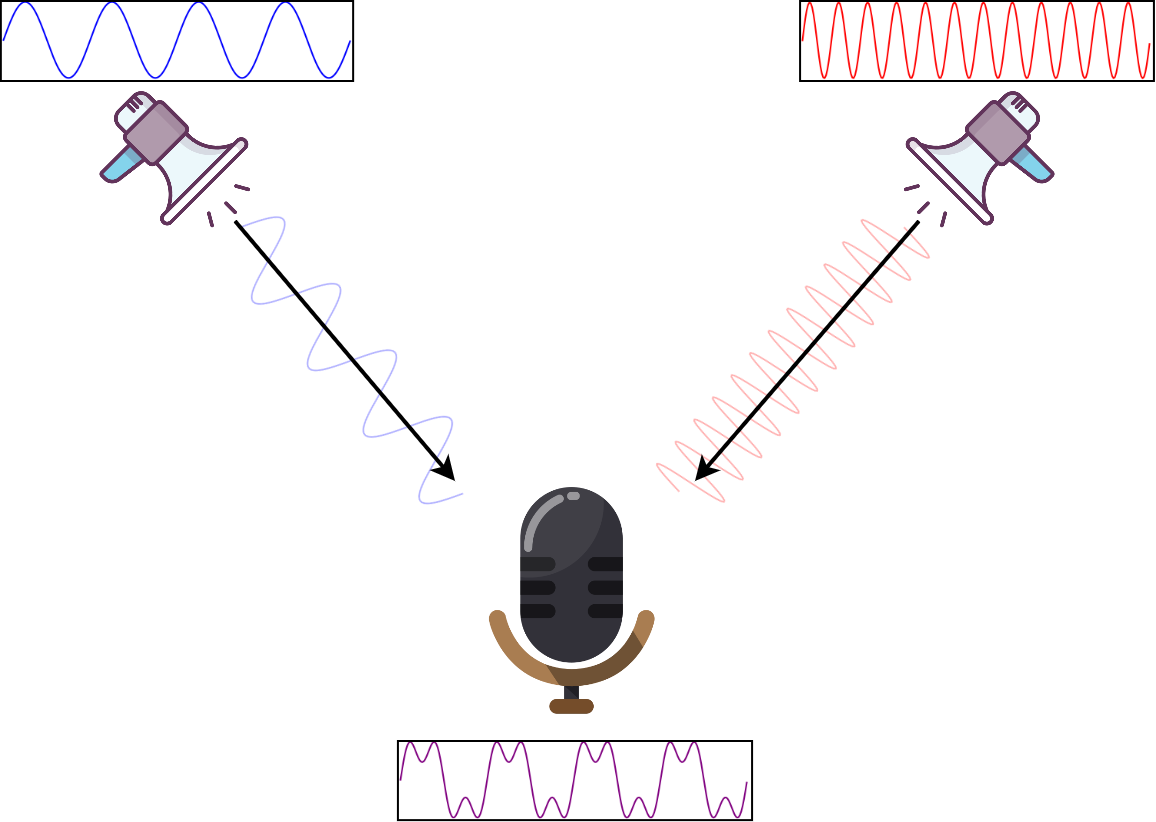
\includegraphics[width=0.7\linewidth]{Images/chap1/superpositionPrinciple.png}
    \captionof{figure}[Superposition of two sound waves]{Superposition of two sound waves arriving simultaneously at the same point in space. The signal in purple, recorded by the microphone, is the sum of the two incoming sound signals, in blue and red. The black arrows illustrate the propagation of the waves from the sound sources to the microphone.}
    \label{fig:superpositionPrinciple}
    \end{center}
\end{figure}

This phenomenon is even more accentuated when a sound wave propagates in an environment with walls and furniture. As illustrated in Fig.~\ref{fig:multipathPropagation}, the sound wave can reflect successively multiple times onto the walls, following a determined path. Moreover, as most sound sources generate spherical waves, leading to a spherical wavefront, the wave propagates in many directions at the same time (illustrated by the multiple arrows coming from the loudspeaker in Fig.~\ref{fig:multipathPropagation}). Because of the many resulting reflections, several delayed copies of the same wave arrive simultaneously at the recording point. Due to the superposition principle, they are added together to the \textit{direct path}, which is the wavefront going directly from the sound source to the receiver. The resulting recorded signal is thus not an exact copy of the original source signal, but rather a combination of delayed and attenuated versions of the original signal. The phenomenon of a signal coming to a receiver from several paths is called \textit{multipath propagation}. The first reflections form what is called \textit{early reflections}, which generally lasts a few milliseconds, until there are ``too many'' of them, which is referred as \textit{reverberation}. Reverberation happens in every closed space, and is more or less accentuated depending on several parameters, such as wall materials or room dimensions. Typically, high reverberation can be heard in churches and cathedrals, while special rooms called \textit{anechoic chambers} have been designed to minimize the effect of reverberation.

\begin{figure}[t]
    \begin{center}
    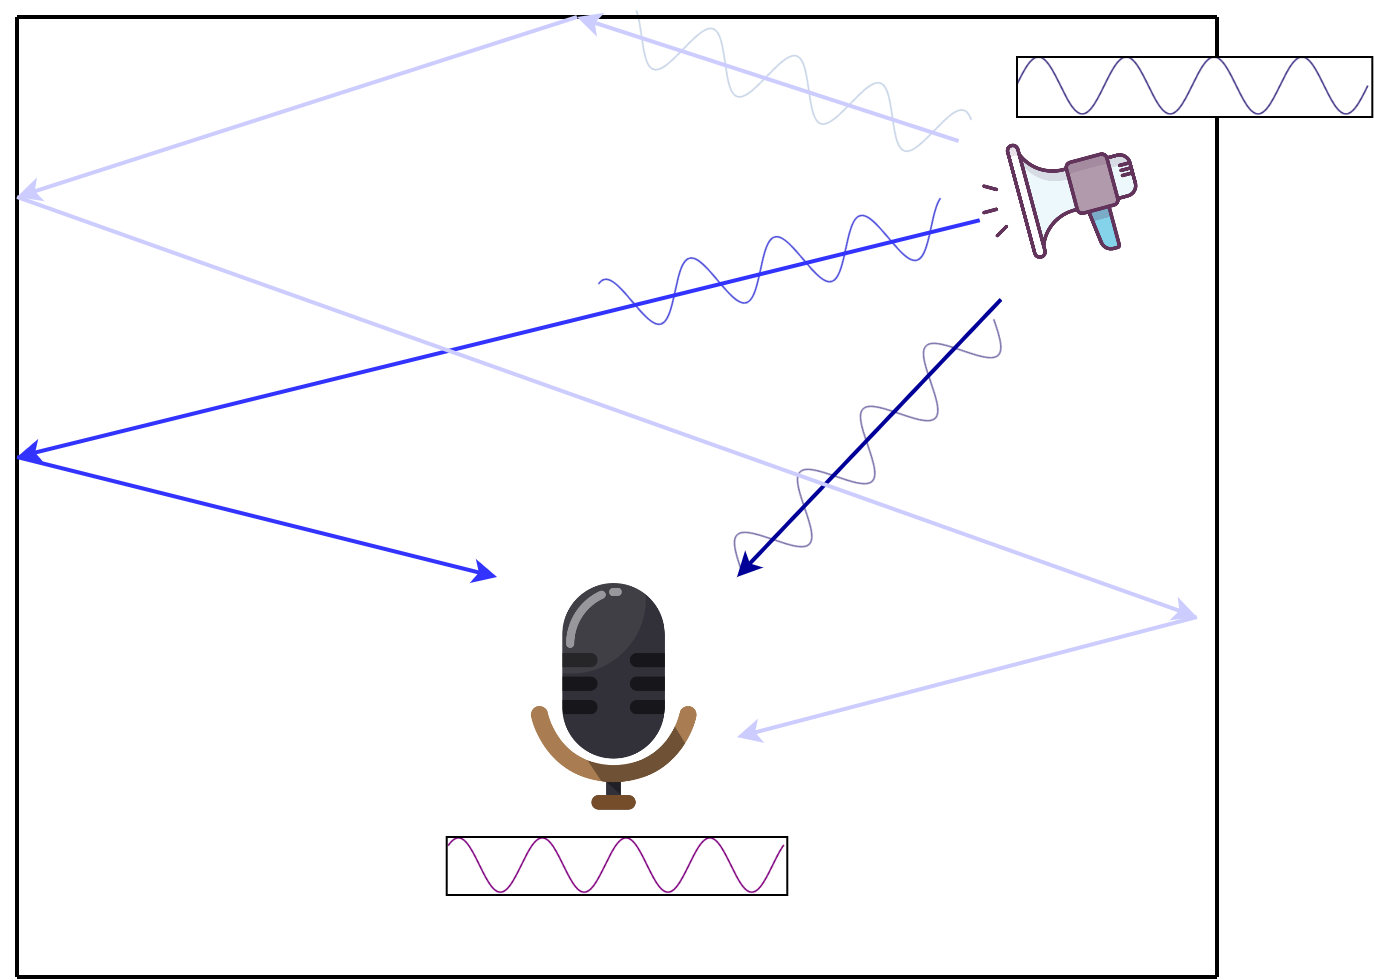
\includegraphics[width=0.6\linewidth]{Images/chap1/multipathPropagation.png}
    \captionof{figure}[Multipath propagation]{Illustration of a multipath propagation, which occurs in the presence of walls where the wavefront of a single sound wave reflects several times onto. The dark blue arrow exhibits the \textit{direct path} from the source to the receiver, and the two other arrows show two different paths that do not arrive at the same time as the direct path. The resulting recorded signal is a combination of all the received waves, delayed from each other because of different path lengths.}
    \label{fig:multipathPropagation}
    \end{center}
\end{figure}

As we can see, the superposition principle makes it difficult to retrieve a clean version of the original sound source signal in a real-world environment. When several sources occur, or when there are reflections in a room, the fact that different sound waves arrive at the recording point makes it very difficult to retrieve the original signals without prior information.


\subsection{Audio signal processing}

For decades, researchers have been trying to reproduce the human hearing abilities using machines. The general motivation of this research effort is to build systems capable of understanding the surrounding sound scene. Such systems require one or more microphones, mimicking the human ears, and signal processing algorithms replacing the brain activity. To accomplish certain goals, usually several algorithms are interconnected into a processing chain, such that each one performs a specific subtask, in order to form a fully-working system. Let us take the example of a system capable of decoding human speech, commonly named automatic speech recognition (ASR) \cite{nassif_speech_2019}. If one can record a perfectly clean speech signal, directly applying an effective ASR algorithm might be sufficient. But in a real-world context, a lot of interference makes the task more complicated. For example, in a domestic environment, other sources (dog barks, TV sound, vacuum cleaning, etc.) could interfere with the target speech signal, as well as surrounding noise coming for example from the outside of an open window. Reverberation is also an important factor that blurs the original speech signal.

To cope with this challenging conditions, several audio signal processing algorithms can be used to clean the recorded speech signal beforehand. As their names refer, \textit{denoising} and \textit{dereverberation} algorithms, often encapsulated as \textit{speech enhancement} \cite{vincent_audio_2018}, aim to remove or at least reduce noise interference and reverberant parts of a signal, respectively. When several sound sources are captured, \textit{source separation} \cite{wang_supervised_2018} aims to separate a mixture signal into several component signals, each one containing the information coming from a single particular source. Source separation techniques can rely on frequency contents, or be obtained by spatial filtering when multiple microphones are used. In the latter type of methods, assuming the knowledge of the target source location, one can spatially filter out the unwanted part of the sound field and extract the sound coming from the target location. However such methods rely on the knowledge of the source location(s), which can be estimated using \textit{sound source  localization} (SSL). To estimate the source(s) location, one needs at least two microphones. SSL algorithms can estimate the directions of one or more overlapping sound sources, and a \textit{source counting} method might be handy to apply beforehand, to ensure that the right number of sources are located in the analyzed signal. Note that when we deal with speech signals, source counting (thus named \textit{speech counting)} is a subtask of \textit{speaker diarization} \cite{anguera_speaker_2012,tranter_overview_2006,park_review_2021}, which is the task aiming to answer the question \textit{who speaks and when ?} in a signal.

\subsection{Thesis focus}

\subsubsection{Speaker counting and localization}
In this thesis, we addressed two of the previously mentioned audio tasks: sound source localization and source counting. More precisely, we deal with speech sources. As stated above, knowing the number of speakers in a signal is a very useful piece of information to extract beforehand. It could prevent the localization algorithm focus onto more sources than the sound really contains, and thus avoid the inclusion of interfering sources, such as noise. Part of this thesis work was thus to design an algorithm capable of counting the number of speakers in challenging acoustic conditions, \emph{i.e.}, in noisy and reverberant environments. The other focus of this thesis was to explore speaker localization in the same kind of challenging environments. Following our interest in counting speakers, we aimed to localize several overlapping speech sources. In order to design robust systems for counting and localizing multiple speakers, our research exploited several tools. 

\subsubsection{Ambisonics format}
Throughout this thesis, we took benefit of the Ambisonics format to represent the sound signal. Such a format is obtained from a spherical microphone array, leading to a multi-channel signal. This more and more adopted audio format presents several great advantages. It is agnostic to the choice of microphone array, that is the encoded signal does not depend on the arrangement of microphones within an array. The sound scene can also be rendered given any disposition of loudspeakers from this format, but this aspect was not of interest in this thesis. Also, it is an isotropic format, meaning that the recording process does not favor any direction. We detail this format in Chapter~\ref{chap:ambisonics}.

\subsubsection{Artificial neural networks}
We explored the potential of artificial neural networks to design robust sound source counting and localization systems. This family of models is part of \textit{deep learning} (DL) \cite{goodfellow_deep_2016}, which is a class of algorithms behind most recent artificial intelligence systems. Their success is due to the ability of neural networks to model complex functions by adjusting their parameters through a learning phase based on a dataset of many examples. They are more and more used today, due to the amount of available data and the increasing computational power to train the algorithms. The basics of artificial neural networks are presented in Chapter~\ref{chap:neuralNetworks}.

%-----------------------------------------------
%  PROBLEM FORMULATION
%-----------------------------------------------
\section{Problem formulation}

In this section, we formulate the problems of counting and localizing sources (regardless whether they are speech or not) in a mathematical framework. The goal is to formally describe the problem we address in this thesis, as well as set the notations we use throughout the chapters. 

\subsection{Mixture model}

We adopt the same mixture model formalization as in \cite{vincent_audio_2018}. Let us assume an environment with $J$ point sources, in which we place a microphone array consisting of $I$ microphones. Each microphone records the sound scene in terms of pressure change from a different position in space, resulting in a multi-channel mixture signal $\mathbf{x}(t)$ containing the recorded signal $x_i(t)$ from each microphone $i$:
\begin{equation}
    \mathbf{x}(t) = \begin{bmatrix} x_1(t) \\ x_2(t) \\ \vdots \\ x_I(t) \end{bmatrix},
\end{equation}
where $t$ denotes discrete time.

As multiple sound sources are present in the environment, according to the superposition principle, each microphone signal is a sum of the signals arriving at the microphone position from each sound source $j$:

\begin{equation}
    x_i(t) = \sum_{j=1}^J c_{ij}(t).
\end{equation}

Here, $c_{ij}(t)$ is the signal arriving at microphone $i$ resulting from the emission of a signal $s_j(t)$ from sound source $j$. The propagation of the source signal and the reverberation of the room has to be taken into account. This can be modeled using a linear time-invariant filter $a_{ij}(\tau)$ if the sources and microphones are static. As all the microphones and sources are at different positions, all filters $a_{ij}$ are distinct. The signal arriving at microphone $i$ can then be expressed as:

\begin{equation}\label{eqSRIR}
    c_{ij}(t) = \sum_{\tau=0}^{+\infty} a_{ij}(\tau) s_j(t-\tau),
\end{equation}
considering a causal filter (\emph{i.e.}, depending only on past and present inputs).
The filters $a_{ij}(\tau)$ are called \textit{room impulse responses} (RIRs) and model the propagation of the source signal from the sound source position to the microphone position, including the reverberation phenomena. The reverberation components are dependent of the source and microphone positions, as well as the room properties (geometry and dimensions, material properties, etc.). Theoretically, a room impulse response is the signal recorded by a perfect microphone (without any noise), coming from a point source emitting an impulse (Dirac distribution), hence the name \textit{room impulse response}.

In real-world environment, noise is an important component which has to be included in the model of the multi-channel mixture signal. Two types of noise can be present in such a recording. On the one hand, we have to take into account the ambient noise which almost always exists in any sound scene. Such a noise is generally considered as a \textit{diffuse source}, which is a source emitting from a whole region in space, as if it was composed of an infinite number of point sources. Examples of diffuse sources include surrounding musical ambience, outside construction works, incomprehensible background conversations (usually referred to as \textit{babble noise}), or even small fluctuations of air. Such diffuse noise can be considered independent of the position in the room, thus common to all microphones. On the other hand, noise modelling the imperfection of each microphone also constitutes an important artifact. Practically, the microphones do not record the world perfectly as it is, and they are not rigorously identical to each other. Therefore, we can incorporate a noise signal $n_i(t)$ for each microphone, including both diffuse noise and microphone-wise noise, to complete the multi-channel mixture signal model:

\begin{equation}
    x_i(t) = \sum_{j=1}^J \sum_{\tau=-\infty}^{+\infty} a_{ij}(\tau) s_j(t-\tau) + n_i(t).
\end{equation}

\subsection{Room impulse responses}

The room impulse responses $a_{ij}(\tau)$ represent the acoustic behavior of the sound according to the emitting and recording positions, as well as the propagation effects induced by the presence of walls or furniture. 

Fig.~\ref{fig:impulseResponse} shows an illustration of a typical RIR. The first and highest peak (in red) represents the \textit{direct path}, which is the straight propagation between the point source and the microphone. The following peaks (in green) are referred to as \textit{early echoes} and encode the beginning of multipath propagation which includes the main reflections from the obstacles. The last part features the \textit{reverberation} phenomenon and results from the superposition of the many late reflections.

\begin{figure}[t]
    \begin{center}
    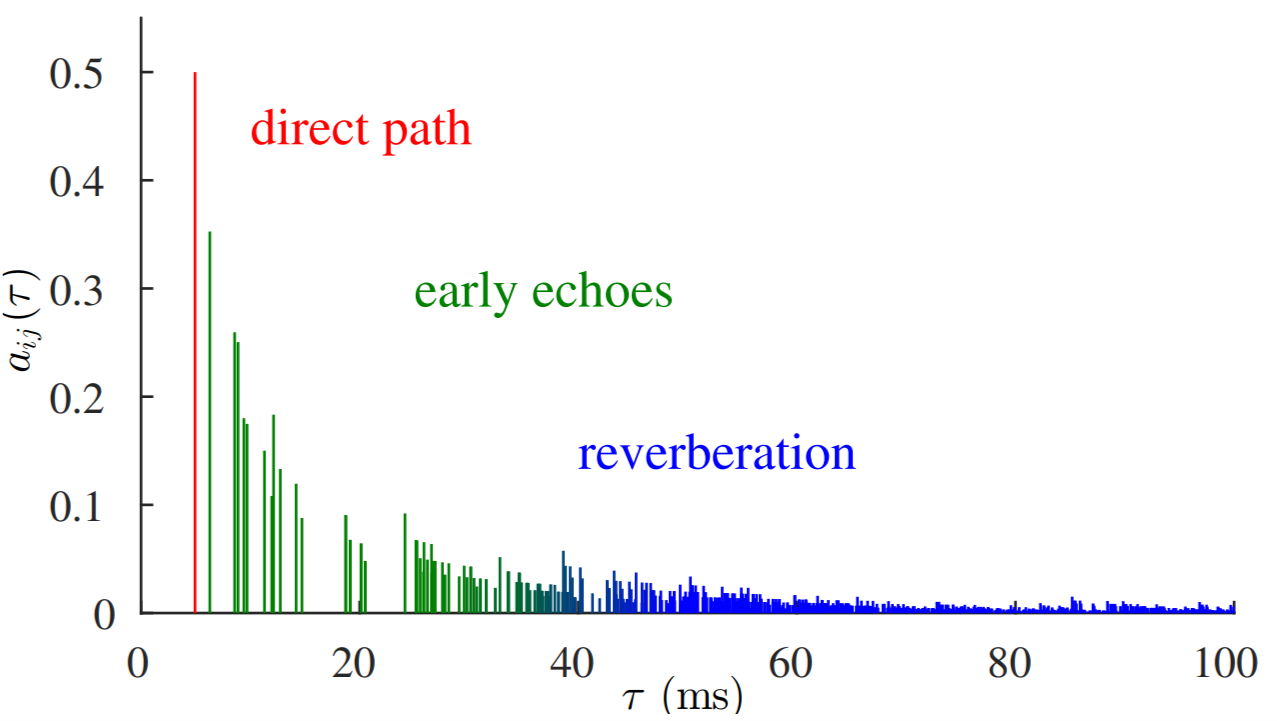
\includegraphics[width=0.6\linewidth]{Images/chap1/impulseResponse.png}
    \captionof{figure}[Illustration of an room impulse response]{Illustration of an room impulse response. Three noticeable parts in an RIR: the direct path (in red), the early echoes (in green) and the reverberation (in blue). Borrowed from \cite{vincent_audio_2018}.}
    \label{fig:impulseResponse}
    \end{center}
\end{figure}

The \textit{reverberation time} (RT60) is a quantity measuring the duration for the impulse response envelop to decrease by $60$~dB. It depends on the room size and the obstacle materials. Typical values of RT60 is between $0.2$ and $0.8$~s for small domestic rooms, and can be higher that $1$~s for larger rooms such as restaurant rooms.

\subsection{Source counting}
\label{ss:sourceCounting}

The number of sources (NoS) $J \in \mathbb{N}$ is an important piece of information which can be useful for several audio processing tasks such as source separation or source localization. For instance, knowing $J$ can improve the performance of separation or localization systems since it can help avoiding ``unwanted'' sound sources (interference). However estimating the number of sources is not straightforward, mainly due to the superposition principle. Fig.~\ref{fig:numberOfSources} illustrates the profile over time of the number of active sources in a 3-source mixture.

\begin{figure}[t]
    \begin{center}
    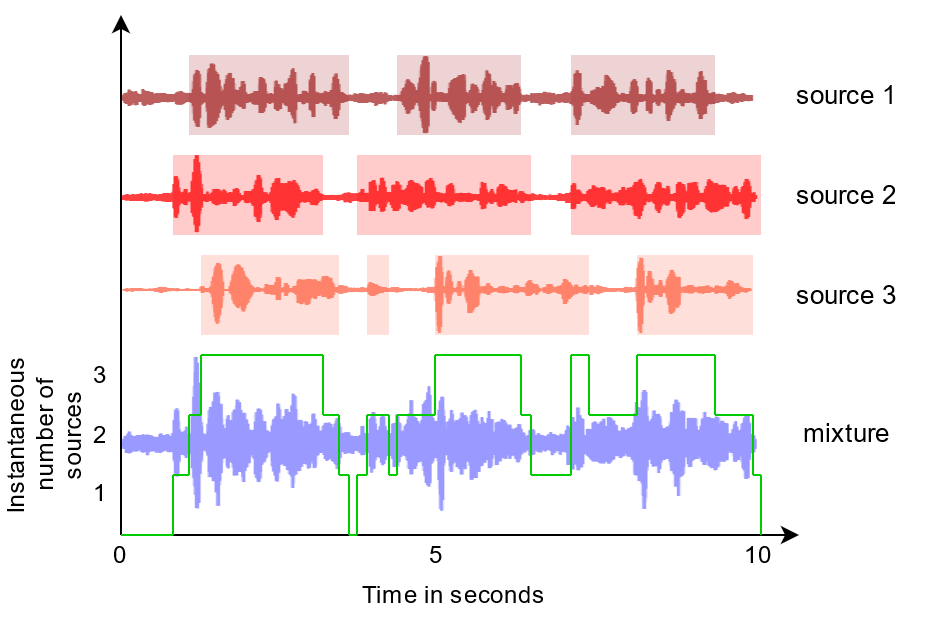
\includegraphics[width=0.8\linewidth]{Images/chap1/numberOfSources.png}
    \captionof{figure}[Example of a time profile of the number of active sources in a 3-source mixture]{Time profile of the number of active sources in a 3-source mixture. The activity of each individual source is represented with rectangles (top). The instantaneous number of active sources in the mixture $J(t)$, resulting from the superposition of each source's activity, is depicted with the green line (bottom).}
    \label{fig:numberOfSources}
    \end{center}
\end{figure}

\textit{Source counting} refers to the problem of estimating the number of sources given a single- or multi-channel mixture signal $\mathbf{x}(t)$. However this problem can be defined according to different levels of temporal resolution. The following NoS quantities can be estimated:

\begin{itemize}
    \item the instantaneous number of sources $J(t)$. The goal is to estimate the NoS at each timestep $t$, depending on the considered temporal resolution (audio sample, time frame). It is at most equal to the total NoS $J$, but it is often lower than $J$ since in general not all sources overlap at the same time;
    \item the maximum number of simultaneous sources $\bar{J}$. It is defined as $\bar{J} = \max_{t} J(t)$, which is the maximum of number of sources which were simultaneously active through the whole analyzed signal;
    \item the total number of sources $J$, which is, as previously defined, the total number of sources involved in the mixture (\textit{i.e.}, they have been active at least once during the analysis). It can be retrieved from $J(t)$ if we are able to identify the sources.
\end{itemize}

In this thesis, we were interested in estimating the instantaneous number of sources. The motivation was to provide a succeeding block in the processing chain (\emph{e.g.}, a localization or tracking algorithm) with an NoS estimate $\tilde{J}(t)$ at any time index $t$. In practice, this necessitates a source counting method operating at high temporal resolution.

Note that when $J=1$, source counting simplifies to the problem of source detection, which is predicting whether a particular source is active ($J(t)=1$) or not ($J(t)=0$) at any time $t$.

When the sources are human speakers (as it is the case in this thesis), source counting is referred to as \textit{speaker counting}, except for $J=1$ for which it is commonly named \textit{voice activity detection} (VAD). When the speech sources need to be identified in addition to counting, this problem is equivalent to \textit{speaker diarization}.

\subsection{Source localization}

The goal of SSL is to derive the spatial positions of the target source(s) based on the recorded multi-channel signal. While multiple microphone arrays can be employed to localize sources, most systems assume the use of only one microphone array, as it is a more practical solution. This problem is not trivial, notably due to the presence of noise as well as reverberation in enclosed spaces. Looking back at Fig.~\ref{fig:multipathPropagation}, we see that several signals originating from the same source arrive at the microphone from different directions. Thus, estimating the actual source direction, and even interpreting the different incoming sound waves as coming from the same point source is not a straightforward task.

Assuming an environment with $J$ emitting sources, the goal of a SSL algorithm is to estimate the position $\mathbf{r}_j(t)$ of each source $j$, given a certain coordinate system, from a multi-channel signal $\mathbf{x}(t)$. Using Euclidian coordinates, $\mathbf{r}_j(t) = (x_j(t), y_j(t), z_j(t))$, while in a spherical domain, $\mathbf{r}_j(t) = (r_j(t), \theta_j(t), \phi_j(t))$, where $r_j$ is the distance, $\theta_j$ the azimuth angle and $\phi_j$ the elevation angle. When only $\theta_j$ and $\phi_j$ are estimated, it is referred to direction-of-arrival (DoA) estimation. Spherical coordinates are especially handy when the microphone is taken as the origin. Cylindrical coordinates are used less often. 

Note that the source positions $\mathbf{r}_j(t)$ are functions of time, as in a general framework the source can be mobile in the surrounding area. In that case, sound source localization can be done with the help of a target tracking system, whose goal is to associate the multiple position estimates and the target sources over time.

%-----------------------------------------------
%  MAIN CONTRIBUTIONS
%-----------------------------------------------
\section{Main contributions}

During three thesis years, our research was focused on speaker counting and localization. Through many experiments, we explored new ways of addressing these tasks in order to improve the existing methods, and tried to analyze their behaviors. Several of these methods led to published/submitted papers:

\begin{itemize}
    \item P.-.A Grumiaux, S. Kiti\'c, L. Girin, A. Guérin, High-resolution speaker counting in reverberant rooms using CRNN with Ambisonics features, \textit{European Signal Processing Conference (EUSIPCO)}, Amsterdam, Netherlands, 2020. 
    \item P.-.A Grumiaux, S. Kiti\'c, L. Girin, A. Guérin, Multichannel CRNN for speaker counting: an analysis of performance, \textit{Forum Acusticum (FA2020)}, Lyon, France, 2020. 
    \item P.-.A Grumiaux, S. Kiti\'c, L. Girin, A. Guérin, Improved feature extraction for CRNN-based multiple sound source localization, \textit{European Signal Processing Conference (EUSIPCO)}, Dublin, Ireland, 2021. 
    \item P.-.A Grumiaux, S. Kiti\'c, P. Srivastava, L. Girin, A. Guérin, SALADnet: Self-Attentive multisource Localization in the Ambisonics Domain, \textit{IEEE Workshop on Applications of Signal Processing to Audio and Acoustics (WASPAA)}, Mohonk Mountain House, New Paltz, NY, 2021.
    \item P.-.A Grumiaux, S. Kiti\'c, L. Girin, A. Guérin, A survey of sound source localization with deep learning methods, Submitted to the Journal of the Acoustical Society of America, 2021.
\end{itemize}

\subsection{Speech counting}

We explored several neural network architectures in order to improve existing methods for speech counting. We showed that relying on multi-channel features (in the Ambisonics format) we could obtain improved speaker counting compared to using single-channel signals. Our method showed great performance to count up to $5$ simultaneous speakers in noisy and reverberant environments, at a short-term frame-wise resolution. This work was presented at the European Conference on Signal Processing in 2020 \cite{grumiaux_high-resolution_2020}. We also conducted several analyses on the performance of neural network architectures according to different hyperparameters, leading to a presentation \cite{grumiaux_multichannel_2020} at the conference Forum Acusticum 2020.

\subsection{Sound source localization literature review}

During our literature review on SSL, which was especially geared towards neural-based methods, a great amount of interesting papers was gathered, annotated and classified. We thoroughly kept collecting more and more deep-learning-based SSL papers, as more and more methods were proposed throughout the years. We finally decided to share this intensive literature review by writing a survey paper on SSL techniques using deep learning \cite{grumiaux_survey_2021}. This paper proposes a classification of neural-based SSL methods according to neural network architectures, types of input features, output paradigms, and learning strategies. It also provides an overview of datasets used for such systems, as well as two summary tables which allow to easily find papers according to specific criteria.

\subsection{Multi-source localization}

We spent several months to address speaker localization with multiple sources in challenging conditions. Using a classification paradigm, we experimented several neural network architectures to improve the localization performance. First, we managed to notably improve the performance of a state-of-the-art system \cite{perotin_crnn-based_2019} and extended it up to 3 speakers, by rethinking the feature extraction\footnote{Note that throughout all this thesis, we refer as feature extraction the first network components which allow to compute a more \textit{high-level} representation of the input features for the remaining part of the network.} part of the network. This work was presented at the European Conference on Signal Processing in 2021 \cite{grumiaux_improved_2021}. We also improved this work by extending the Ambisonics order of the multi-channel recording. We then explored the benefit of self-attention models for an attempt to remove the recurrent layers, known to be computationally cumbersome. Not only did we successfully manage to replace the recurrent part with self-attention, but we also slightly improved the localization performance. This work has been accepted for presentation at the Workshop on Applications of Signal Processing to Audio and Acoustics \cite{grumiaux_saladnet_2021}. We finally assessed the benefit of using more microphones to record the analyzed signal, \emph{i.e.}, increasing the Ambisonics order (see Chapter~\ref{chap:ambisonics}). The results clearly demonstrated the improvement of the localization performance in this configuration, at the cost of more recorded data.

\subsection{Exploration of a new type of input features for localization}

Based on a pioneering work \cite{daniel_time_2020} introducing a new type of Ambisonics representation called time-domain velocity vector (TDVV), we carried out a lot of experiments to take benefit of this new feature for SSL. As it was an exploratory idea, we limited our experiments to single-source configuration, with the intention to extend the models to multi-source signals when reaching conclusive results. We tried many neural networks architectures, including dilated convolutions, residual connections, self-attention mechanisms. We also explored several approaches to estimate the TDVV as it is not a straightforward feature to derive.

While the models trained with this new representation were able to localize one source at a fair precision, we never managed to demonstrate the superiority of this new input feature for single-source localization compared to the use of intensity-based features. Although this series of experiments was not conclusive, we nevertheless present all our results in this document, and try to find out what was missing to take the most out of this new idea.

\subsection{Combination of speech counting and localization}

After exploring new ideas regarding speaker counting and localization, we proposed several systems combining both tasks, either sequentially or jointly. First, we showed that estimating the number of speakers with a neural network allows better localization performance than if it is derived solely from the localization output. We also observed that the performance is still satisfactory compared to the use of a ground-truth NoS. Next, we evaluated the benefit of using the estimated NoS as an additional input feature for the localization network. Finally, we proved that it is possible to train a neural network to jointly estimate the number of sources and their positions, with high counting and localization accuracies.

%-----------------------------------------------
%  MANUSCRIPT OUTLINE
%-----------------------------------------------
\section{Manuscript outline}

The remainder of this document is organized as follows. Chapter~\ref{chap:ambisonics} introduces the concept of spherical harmonics and the Ambisonics representation. The intensity features, frequency-domain and time-domain velocity vectors are also derived. In Chapter~\ref{chap:neuralNetworks}, we quickly present the different neural network architectures used in our experiments, with an emphasis on less common mechanisms, such as residual connections or multi-head self-attention. We then provide a literature review on source counting and sound source localization, focused on neural-based methods, in Chapter~\ref{chap:soa}. The following chapters detail the experiments conducted during the three years of this thesis. Our models and their analyses for speaker counting are explained in Chapter~\ref{chap:counting}. In Chapter~\ref{chap:tdvv} we present our attempts to improve single-source localization using the TDVV, while in Chapter~\ref{chap:multisourceLocalization} we describe our work on multi-source localization using more usual features. Next, Chapter~\ref{chap:countingLocalization} presents our investigations towards a neural model for joint speaker counting and localization. Finally, we conclude this thesis in Chapter~\ref{chap:conclusion}.


\chapter{Ambisonics}
\label{chap:ambisonics}

%-----------------------------------------------
%   INTRODUCTION
%-----------------------------------------------

\lettrine{T}{he} Ambisonics format is an audio format capable of efficiently representing the spatial aspect of a sound field. Hence, it has become a popular format for 3D spatial audio coding \cite{pulkki_parametric_2018}, as a \emph{de facto} standard in both professional and consumer domains \cite{herre_mpeg-h_2014} (see also the Facebook 360\footnote{https://facebook360.fb.com/spatial-workstation/} and the Google360\footnote{https://support.google.com/youtube/answer/6395969} systems available online).
Ambisonics finds its roots in the 1930s, when Blumlein's original work \cite{blumlein_improvements_1931} on coincident stereo recordings proposed to place two figure-of-eight microphones in a orthogonal manner. Gerzon \cite{gerzon_periphony_1973} extended this idea in the 1970s by theorizing what we call the first-order Ambisonics (FOA) format, originally known as B-format, which paved the path to high-order Ambisonics (HOA) \cite{daniel_representation_2001}.

While the term Ambisonics arose from the design of the corresponding microphones, we also often encounter terms related to the spherical harmonics theory in the literature. In fact, the Ambisonics representation consists of the coefficient of the spherical harmonics decomposition of the signal. In this thesis, we will use the term Ambisonics because of the past of the laboratory we conducted our research in, but in this chapter we show how both theories are linked together.

In this chapter, we establish the theoretical foundations of the Ambisonics format, which we adopted to represent audio signals in this thesis. After briefly explaining why this format is of interest, we derive the spherical harmonics decomposition of the solution of the wave equation. This decomposition leads us to the definition of first-order and higher-order Ambisonics. We finally discuss several representations derived from the Ambisonics format, useful for sound scene analysis: the pseudointensity vector, the frequency-domain velocity vector, and the time-domain velocity vector.

An interesting reader may find more in-depth details in diverse references, \emph{e.g.}, theses \cite{daniel_representation_2001,merimaa_analysis_2006,baque_analyse_2017,moreau_etude_2006}, or books \cite{zotter_ambisonics_2019, rafaely_fundamentals_2019, jarrett_theory_2017, williams_fourier_2000}.

%-----------------------------------------------
%   INTEREST OF THE AMBISONICS FORMAT
%-----------------------------------------------
\section{Interest of the Ambisonics format}

One of the main benefits of the Ambisonics lies in its capability of compactly encoding the surrounding sound scene in a format that is theoretically agnostic regarding the configuration of the recording microphone array. Likewise, the Ambisonics format is flexible with respect to the setup of an audio system used for reproduction, as its decoding can be adapted to match the given layout, \emph{e.g.}, to headphones, stereo monitors, 5.1 audio systems, or even a setup with many loudspeakers \cite{zotter_ambisonics_2019}. The Ambisonics format is an isotropic representation of the sound field, \emph{i.e.}, the encoding takes equally into account all spatial directions. It contains the directional information of the sound sources, due to the microphones nature and orientation. A particularity of this characteristics is that it becomes very handy to perform some transformations of the encoded sound recording: for instance, one can easily rotate the sound field by multiplying the multi-channel recording by the appropriate matrix. One typical application of such a property is to take into account the movement of a robot's head when localizing surrounding sounds.

Due to these advantages, more and more commercial applications opt for this sound representation to handle audio signals. As we have seen above, internet giants such as Google or Facebook use the Ambisonics format for their spatial audio applications, especially in virtual reality (VR) environments. Recently, we have witnessed an increase of available easy-to-use devices that can be used to record spatial audio in the Ambisonics format (see Fig.~\ref{fig:ambisonics_microphones}): mh acoustics' EigenMike,\footnote{https://mhacoustics.com/products\#eigenmike1} Zoom's H3-VR recorder,\footnote{https://zoomcorp.com/fr/fr/enregistreurs-portatifs/handheld-recorders/h3-vr-360-audio-recorder/} Zylia's ZM-1.\footnote{https://www.zylia.co/zylia-zm-1-microphone.html} Decoding tools are also largely available nowadays, especially to be used in digital audio workstations (DAW): IEM plug-in suite,\footnote{https://plugins.iem.at/} b<>com plug-ins,\footnote{https://b-com.com/en/process/spatial-audio-family} IRCAM's Panoramix,\footnote{https://forum.ircam.fr/projects/detail/panoramix/} or Noise Makers' Ambi Head HD\footnote{https://www.noisemakers.fr/ambi-head-hd/} to name a few.

\begin{figure}[t]
    \begin{center}
    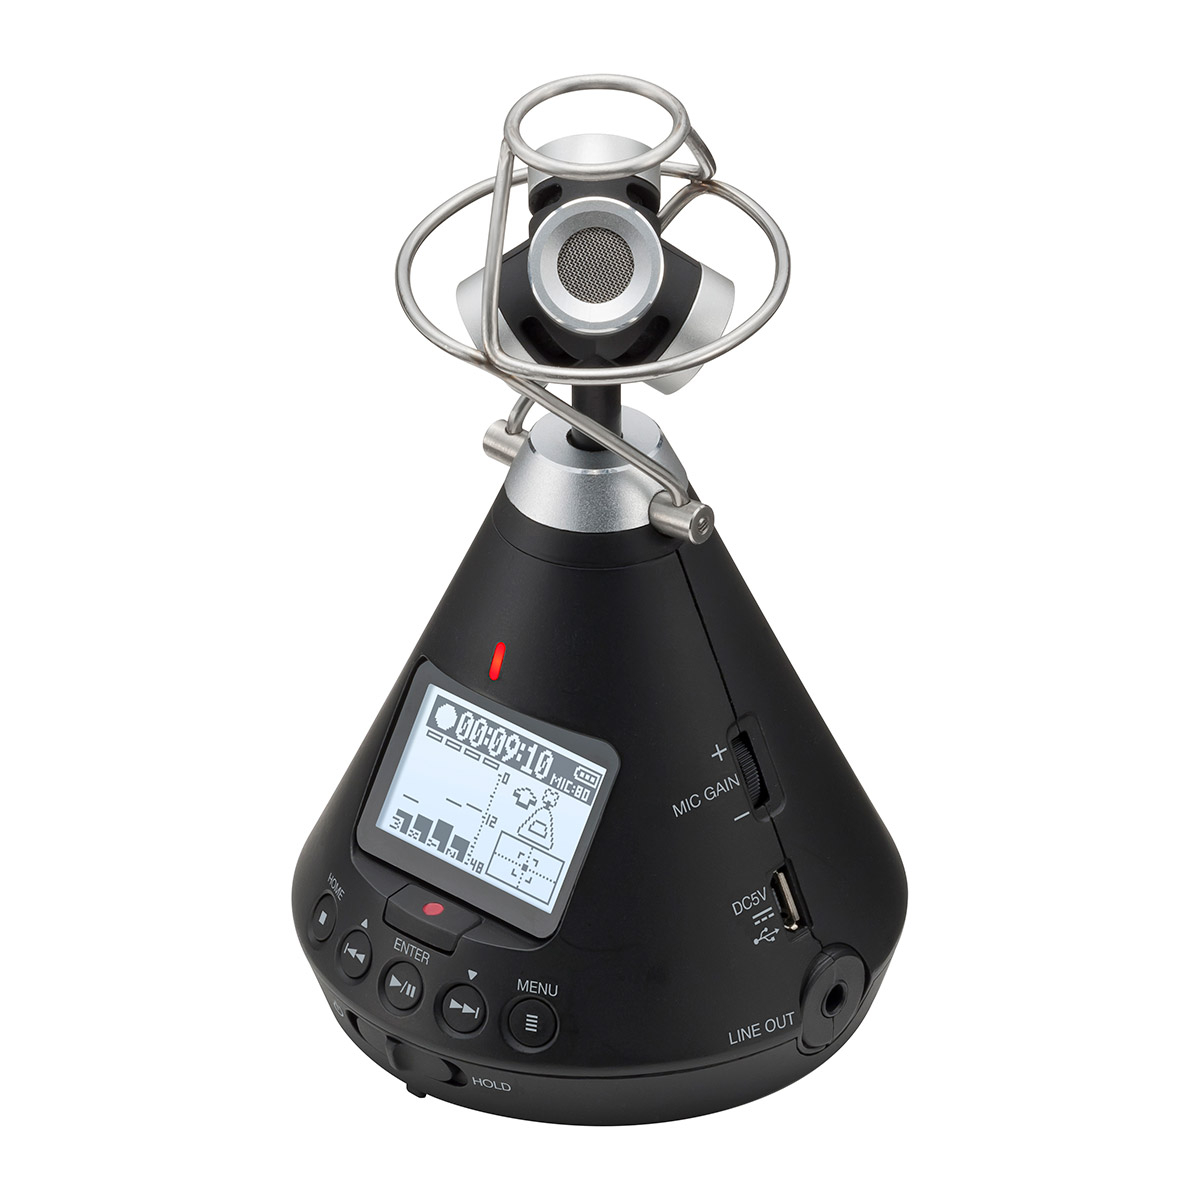
\includegraphics[width=0.35\linewidth]{Images/chap2/h3-vr.jpg}
    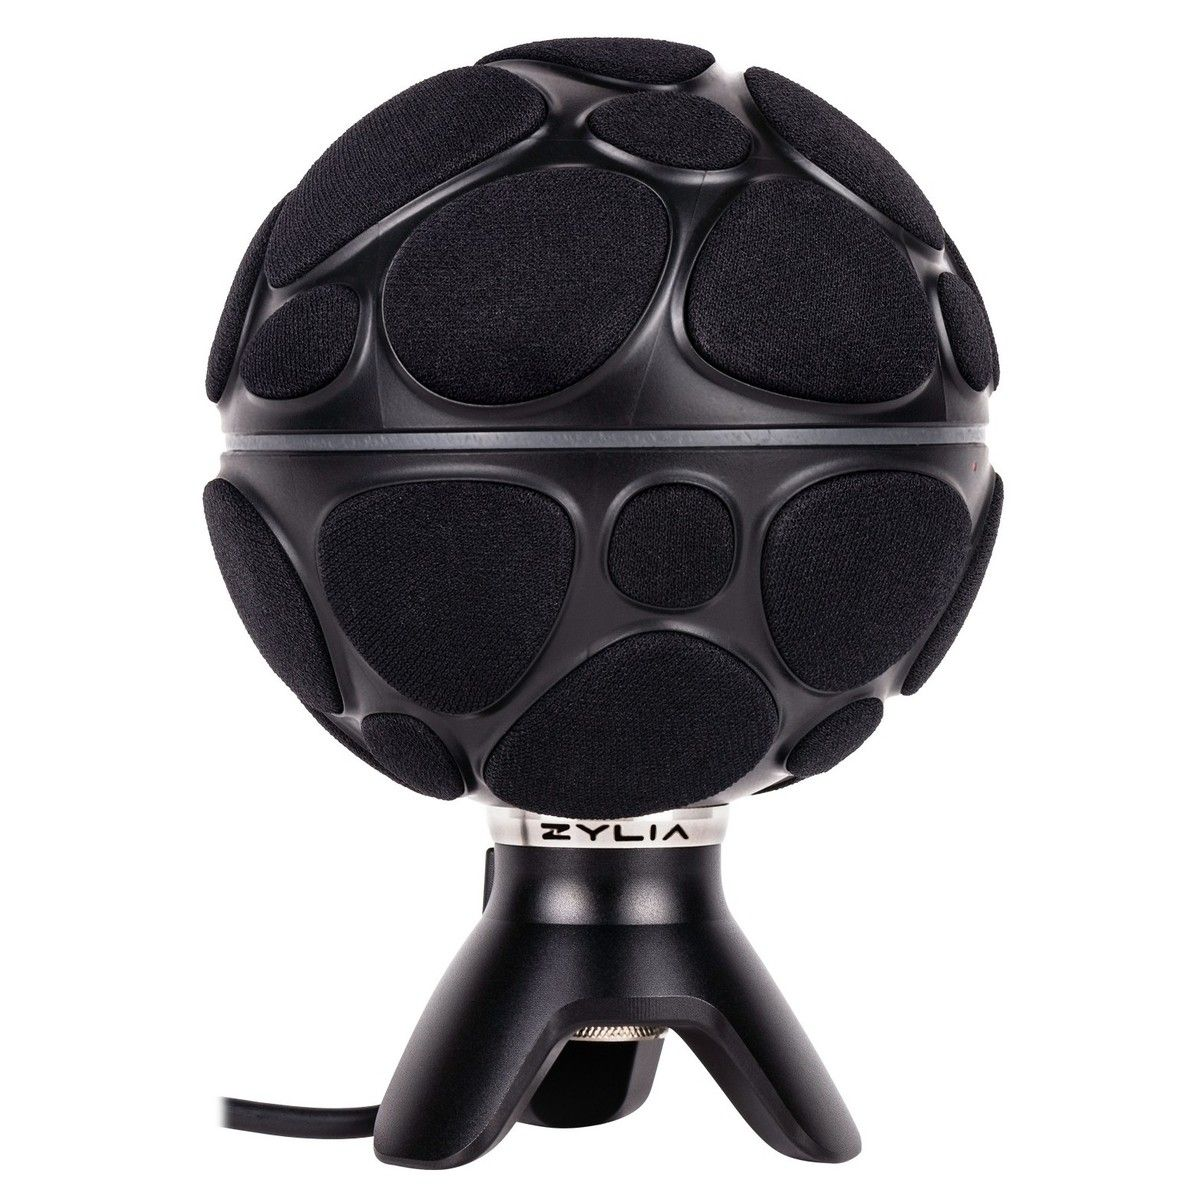
\includegraphics[width=0.35\linewidth]{Images/chap2/zm-1.jpg}
    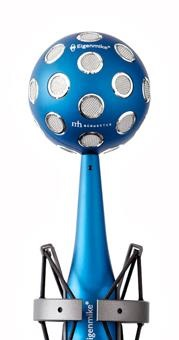
\includegraphics[width=0.2\linewidth]{Images/chap2/eigenmike.jpg}
    \captionof{figure}[Examples of Ambisonics microphone arrays]{Examples of microphone arrays suitable for the encoding of the recorded sound field into the Ambisonics format. \textbf{Left}: Zoom's H3-VR (4 capsules, Ambisonics format up to order 1); \textbf{middle}: Zylia's ZM-1 (19 capsules, up to order 3); \textbf{right}: mh acoustics' EigenMike (32 capsules, up to order 4).}
    \label{fig:ambisonics_microphones}
    \end{center}
\end{figure}

%-----------------------------------------------
%   WAVE EQUATION AND SHD
%-----------------------------------------------
\section{Wave equation and spherical harmonics decomposition}

In this section, we derive the solution of the wave equation in the spherical domain and exhibit the spherical harmonics decomposition of the sound signal, which will lead to the definition of the Ambisonics format in the section~\ref{sec:ambisonics}.

\subsection{Wave equation solution in the spherical domain}

A sound signal is the evolution of the sound pressure $p(\mathbf{r},t)$ with time $t$ at the recording point $\mathbf{r}$, which is measured in Pascals (Pa). The recorded signal is due to the sound source which produces a sound wave, \emph{i.e.}, the solution of the famous \textit{acoustic wave equation} :
\begin{equation}
\label{eq:waveEquation}
    \nabla^2 p(\mathbf{r},t) - \frac{1}{c^2} \frac{\partial^2}{\partial t^2} p(\mathbf{r},t) = 0,
\end{equation}
where $\nabla^2$ denotes the Laplacian operator and $c$ is the speed of sound in the considered fluid (in the air, $c = \SI{343}{\meter\per\second}$ at $\SI{20}{\degreeCelsius}$).

We want to find the general solution of the wave equation in the three-dimensional space. To do that, we represent the 3D space using spherical coordinates, \emph{i.e.}, ${\mathbf{r} = (r, \theta, \phi)}$, where $\theta$ is the azimuth angle and $\phi$ the elevation angle, as illustrated in Fig.~\ref{fig:spherical_coordinates}. The following equations describe the relationship between cartesian and spherical coordinates:
\begin{equation}
\label{eq:spherical_coordinates}
    \left\{ 
    \begin{aligned} 
      x &= r \cos\theta \cos\phi \\
      y &= r \sin\theta \cos\phi. \\
      z &= r \sin\phi
    \end{aligned}
    \right.
\end{equation}

\begin{figure}[t]
    \begin{center}
    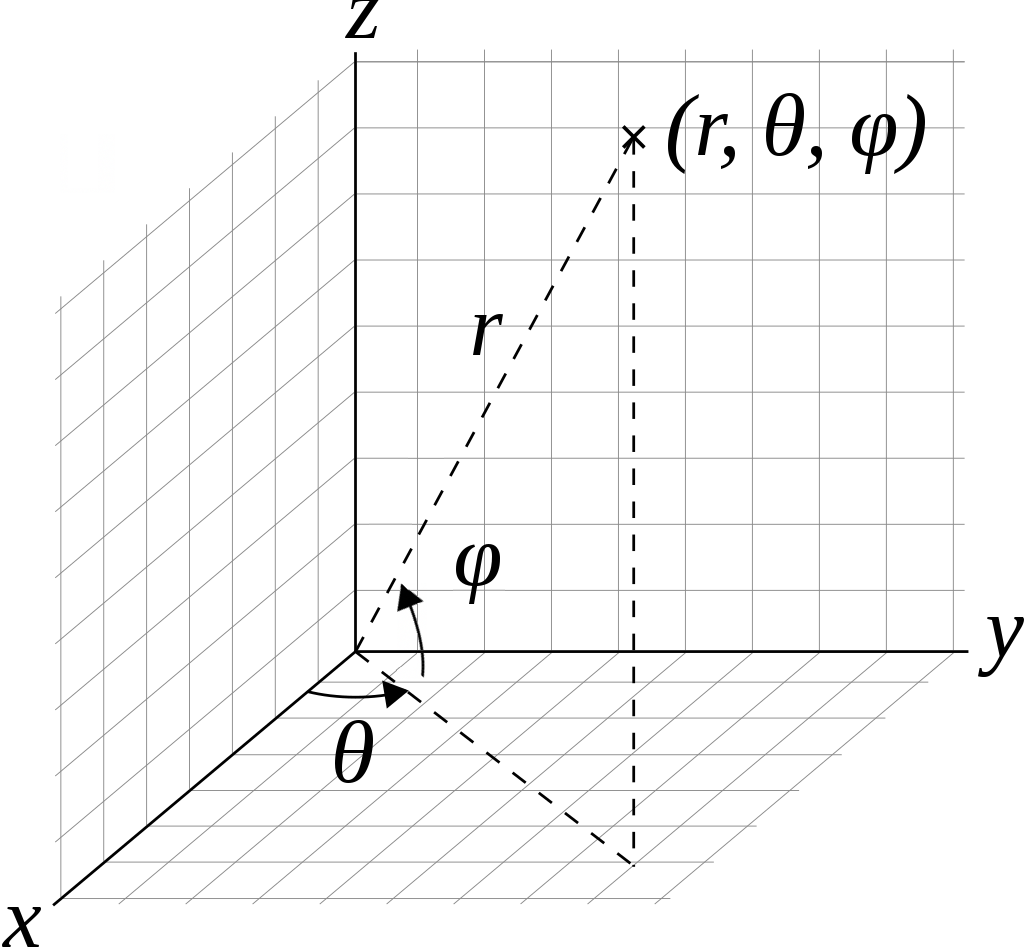
\includegraphics[width=0.4\linewidth]{Images/chap2/spherical_coordinates.png}
    \captionof{figure}[Spherical coordinate system]{Spherical coordinate system. Any position in space can be described with three numbers: the distance $r$, the azimuth angle $\theta$ and the elevation angle (or polar angle) $\phi$. The relation between spherical coordinates $r,\theta, \phi$ and cartesian coordinates $x,y,z$ is given by \eqref{eq:spherical_coordinates}. Borrowed from \href{https://commons.wikimedia.org/wiki/File:3D_Spherical_2.svg}{Dmcq, CC BY-SA 3.0}.}
    \label{fig:spherical_coordinates}
    \end{center}
\end{figure}

In three dimensions, using spherical coordinates, the Laplacian operator for a function $f(r,\theta,\phi)$ is given by:
\begin{equation}
\label{eq:sphericalLaplacian}
    \nabla_\mathbf{r}^2 f = \frac{1}{r^2} \frac{\partial}{\partial r} \bigg(r^2 \frac{\partial f}{\partial r} \bigg) + \frac{1}{r^2 \sin\theta} \frac{\partial}{\partial \theta} \bigg(\sin\theta \frac{\partial f}{\partial \theta} \bigg) + \frac{1}{r^2 \sin^2 \theta} \frac{\partial^2 f}{\partial \phi^2}.
\end{equation}

To derive a solution for the wave equation in the spherical domain, one can proceed to a separation of variables, \emph{i.e.}, we assume that $p$ takes the form:
\begin{equation}
    \label{eq:separationVariables}
    p(r,\theta,\phi,t) = R(r)\Theta(\theta)\Phi(\phi)T(t).
\end{equation}
Then, by injecting \eqref{eq:separationVariables} in \eqref{eq:waveEquation} using \eqref{eq:sphericalLaplacian}, we obtain one separate partial equation for each variable $r$, $\theta$, $\phi$ and $t$ \cite[p.~35]{rafaely_fundamentals_2019}:
\begin{equation}
\label{eq:partialEquationR}
    r^2 \frac{d^2}{dr^2} R + 2r \frac{d}{dr} R + \big[(kr)^2 - n(n+1)\big] R = 0,
\end{equation}
with $k=\frac{\omega}{c}$ being the wave number of the sound wave ($\omega = 2 \pi f$ is the angular frequency),
\begin{equation}
\label{eq:partialEquationTheta}
      \frac{d}{d \mu} \bigg[(1-\mu^2)\frac{d}{d \mu} \Theta \bigg] + \bigg[n(n+1) - \frac{m^2}{1-\mu^2} \bigg] \Theta = 0,
\end{equation}
with $\mu = \cos^2 \theta$ and $\lvert m \rvert \leq n, m \in \mathbb{Z}, \; n \in \mathbb{N}$,
\begin{equation}
\label{eq:partialEquationPhi}
      \frac{d^2 \Phi}{d \phi^2} + m^2 \Phi = 0,
\end{equation}
and
\begin{equation}
\label{eq:partialEquationT}
      \frac{d^2 T}{dt^2} + \omega^2 T = 0, \quad \omega \in \mathbb{R}.
\end{equation}
\eqref{eq:partialEquationPhi} and \eqref{eq:partialEquationT} immediately lead to the following exponential solutions, valid for an harmonic wave, \emph{i.e.}, with a single frequency $\omega$ :
\begin{equation}
    T(t) = e^{i \omega t},
\end{equation}
and 
\begin{equation}
    \Phi(\phi) = e^{i m \phi},
\end{equation}
where $i = \sqrt{-1}$. Note that $m$ is an integer because $\Phi$ is $2 \pi$-periodic.
\eqref{eq:partialEquationTheta} is known as the associated \textit{Legendre differential equation}, whose non-singular solutions are given by the associated \textit{Legendre functions of the first kind} \cite[p.~715]{arfken_mathematical_2013}:
\begin{equation}
    \Theta(\theta) = P_n^m(\cos\theta), \quad m \in \mathbb{Z}, n \in \mathbb{N}.
\end{equation}
\eqref{eq:partialEquationR} is referred as the \textit{spherical Bessel equation}, whose solutions are a weighted combination of the \textit{spherical Bessel functions of the first kind} $j_n(kr)$ and the \textit{spherical Hankel functions of the first kind} $h_n(kr)$:
\begin{equation}
    R(r) = R_1 j_n(kr) + R_2 h_n(kr),
\end{equation}
with $R_1$, $R_2 \in \mathbb{R}$. In fact, in our case, we have necessarily $R_2=0$ since the functions $h_n$ diverge at $r=0$ and we suppose that no infinite sound pressure occurs at the recording point.

Finally, combining these variable-wise equations leads to the set of fundamental solutions for the wave equation in the spherical domain :
\begin{equation}
\label{eq:solutionWaveEquation}
    p(\mathbf{r},t) = R_1 j_n(kr) P_n^m(\cos \theta) e^{im\phi} e^{iwt},
\end{equation}
with $n \in \mathbb{N}$, $m \in \mathbb{Z}$ and $\lvert m \rvert \leq n$. The general solution is a weighted sum of these fundamental solutions. The products formed by the angular factors $P_n^m(\cos \theta)$ and $e^{im\phi}$ are known to be the (scaled) \textit{spherical harmonics}, which brings us to the next subsection.

\subsection{Spherical harmonics}

\subsubsection{Complex spherical harmonics}

The terms depending on $\theta$ and $\phi$ on the wave equation solutions \eqref{eq:solutionWaveEquation} are grouped together to define the complex spherical harmonics. This set of complex functions, indexed by $n$ and $m$, are defined on the unit sphere by \cite[p.~4]{rafaely_fundamentals_2019}:
\begin{equation}
    Y_n^m(\theta,\phi) = \sqrt{\frac{2n+1}{4 \pi} \frac{(n-m)!}{(n+m)!}} P_n^m(\cos\theta) e^{i m \phi},
\end{equation}
where $n \in \mathbb{N}$ is the order, and $m \in \{-n, -n+1, ..., n-1, n\}$ is the degree of the spherical harmonic. We recognize the associated Legendre functions as well as the exponential function of the elevation $\phi$.

An interesting property of these complex spherical harmonics is that they form an orthonormal basis of the Hilbert space $L_2(S^2)$ (\emph{i.e.}, the set of all square-integrable complex functions of the unit sphere), with the following inner product:
\begin{equation}
    \langle f \mid g \rangle = \frac{1}{4 \pi} \int_{\theta=0}^{2 \pi} \int_{\phi=-\frac{\pi}{2}}^{\frac{\pi}{2}} f(\theta,\phi) g(\theta,\phi)^* \cos \phi d \phi d \theta,
\end{equation}
where $*$ denotes the complex conjugates.
This property involves that any function $f(\theta,\phi)\in L_2(S^2)$ can be decomposed as a weighted sum of spherical harmonics:
\begin{equation}
    f(\theta,\phi) = \sum_{n=0}^{\infty} \sum_{m=-n}^{n} f_{nm} Y_n^m(\theta,\phi),
\end{equation}
with $f_{nm}$ denoting the coefficients of $f(\theta,\phi)$ on this basis. This representation is known as the \textit{spherical harmonics decomposition} (SHD) of $f(\theta,\phi)$. The coefficients $f_{nm}$ can be computed as:
\begin{equation}
    \begin{split}
    f_{nm} &= \langle f(\theta,\phi) \mid Y_n^m(\theta,\phi) \rangle \\
           &= \int_{\theta=0}^{2 \pi} \int_{\phi=-\frac{\pi}{2}}^{\frac{\pi}{2}} f(\theta,\phi) Y_n^m(\theta,\phi)^* \cos\phi d \phi d \theta.
    \end{split}
\end{equation}

From \eqref{eq:solutionWaveEquation}, we can express the general solution (linear sum of fundamental solutions) of the wave equation on the basis of spherical harmonics:
\begin{equation}\label{eqHOAdecomp}
    p(\theta,\phi,r,t) = \sum_{n=0}^{\infty} \sum_{m=-n}^n \alpha_{nm} j_n(kr) Y_n^m(\theta,\phi) e^{i \omega t},
\end{equation}
where $\alpha_{nm} \in \mathbb{R}$ are the weights of each fundamental solution. 

\subsubsection{Real spherical harmonics}
\label{sec:realSphericalHarmonics}

\textit{Real} spherical harmonics $\tilde{Y}_n^m$ also exist and are defined by \cite[p.~28]{jarrett_theory_2017}:
\begin{equation}
\label{eq:realSphericalHarmonicsDefinition}
    \tilde{Y}_n^m(\theta,\phi) = (-1)^{\lvert m \rvert} \sqrt{\frac{2n+1}{4 \pi} \frac{(l-\lvert m \rvert)!}{(l+\lvert m \rvert)!}} P_n^{\lvert m \rvert}(\cos\theta) 
    \begin{cases}
        \sqrt{2} \sin(\lvert m \rvert \phi), & \text{if $m<0$}\\
        1, & \text{if $m=0$}. \\
        \sqrt{2} \cos(m \phi), & \text{if $m>0$}\\
    \end{cases}
\end{equation}

The real spherical harmonics $\tilde{Y}_n^m$ can be derived from the complex spherical harmonics by:
\begin{equation}
    \tilde{Y}_n^m(\theta,\phi) = 
    \begin{cases}
        \sqrt{2} (-1)^m \mathfrak{I} (Y_n^{-m}(\theta,\phi)), & \text{if $m<0$} \\
        Y_n^0(\theta,\phi), & \text{if $m=0$}, \\
        \sqrt{2} (-1)^m \mathfrak{R} (Y_n^m(\theta,\phi)), & \text{if $m>0$}
    \end{cases}
\end{equation}
where $\mathfrak{R}(\cdot)$ and $\mathfrak{I}(\cdot)$ denote the real and imaginary parts of the argument, respectively.
Inversely, the complex spherical harmonics $Y_n^m$ can be obtained from the real spherical harmonics:
\begin{equation}
\label{eq:real2complex}
    Y_n^m(\theta,\phi) = 
    \begin{cases}
        \frac{1}{\sqrt{2}} (\tilde{Y}_n^{-m}(\theta,\phi) - i \tilde{Y}_n^m(\theta,\phi)), & \text{if $m<0$} \\
        \tilde{Y}_n^0(\theta,\phi), & \text{if $m=0$}. \\
        \frac{1}{\sqrt{2}} (-1)^m (\tilde{Y}_n^m(\theta,\phi) + i \tilde{Y}_n^{-m}(\theta,\phi)), & \text{if $m>0$}
    \end{cases}
\end{equation}
The real-valued spherical harmonics also form an orthogonal basis of the set of real functions on the unit sphere, using the inner product \cite[p.~302]{daniel_representation_2001}:
\begin{equation}
    \langle f \mid g \rangle = \frac{1}{4 \pi} \int_{\theta=0}^{2 \pi} \int_{\phi=-\frac{\pi}{2}}^{\frac{\pi}{2}} f(\theta,\phi) g(\theta,\phi) \sin \phi d \phi d \theta.
\end{equation}

An orthonormal basis can be defined by scaling each real spherical harmonic $\tilde{Y}_n^m$ by $\sqrt{2n+1}$ \cite{daniel_representation_2001}, and similarly to the complex spherical harmonics, we can decompose any real function $f(\theta,\phi)$ on the unit sphere on this basis:
\begin{equation}\label{eqHOArealDecomp}
    f(\theta,\phi) = \sum_{n=0}^\infty \sum_{m=-n}^{n} f_{nm} \tilde{Y}_n^m(\theta,\phi),
\end{equation}
where $f_{nm}$ are the coefficients of the decomposition.

\subsection{Wave equation solution for a single plane wave}

To define the Ambisonics components from the wave equation solution, we focus on deriving the solution for a single plane wave, and then we deduce the expression in the general case. We consider a single-frequency plane wave arriving from direction $(\theta_k,\phi_k)$, with amplitude $B$ and wave number $k=\frac{\omega}{c}$, $\omega = 2 \pi f$ where $f$ is the frequency of the wave. This plane wave also satisfies the general solution of the wave equation, and it can be shown that in this case the solution can be written as \cite[p.~227]{williams_fourier_2000}:
\begin{equation}
    p(r,\theta,\phi,t) = 4 \pi B e^{i \omega t} \sum_{n=0}^{\infty}  i^n  j_n(kr) \sum_{m=-n}^n Y_n^m(\theta,\phi) Y_n^m(\theta_k,\phi_k)^*.
\end{equation}

Using the relation between real and complex spherical harmonics in \eqref{eq:real2complex}, we can express the sum containing complex spherical harmonics in terms of real spherical harmonics:
\begin{equation}
    \sum_{m=-n}^n Y_n^m(\theta,\phi) Y_n^m(\theta_k,\phi_k)^* = \sum_{m=-n}^n \tilde{Y}_n^m(\theta,\phi) \tilde{Y}_n^m(\theta_k,\phi_k),
\end{equation}
leading to the expression of the pressure for the single plane wave, using real spherical harmonics:
\begin{equation}
\label{eq:planeWaveDecomposition}
    p(r,\theta,\phi,t) = B e^{i \omega t} \sum_{n=0}^{\infty}  i^n  j_n(kr) \sum_{m=-n}^n \tilde{Y}_n^m(\theta,\phi) \tilde{Y}_n^m(\theta_k,\phi_k),
\end{equation}
where the constant term $4 \pi$ has been incorporated in the amplitude term $B$. This last expression for the solution of the wave equation in the spherical domain (for a single plane wave) brings us to the definition of the Ambisonics coefficients.
%-----------------------------------------------
%   FOA & HOA
%-----------------------------------------------

\section{First-order and higher-order Ambisonics}
\label{sec:ambisonics}

\subsection{Definition of Ambisonics coefficients}

\eqref{eq:planeWaveDecomposition} exhibits a solution of the wave equation for a single-frequency plane wave of amplitude $A$, angular frequency $\omega$ and coming from direction $(\theta_k,\phi_k)$. The Ambisonics coefficients are defined as the coefficients of the decomposition of the pressure $p$ on the basis of real spherical harmonics \cite{daniel_representation_2001}:
\begin{equation}\label{eqPlaneWaveCf}
    B_n^m(t) = B e^{i \omega t} \tilde{Y}_n^m (\theta_k,\phi_k).
\end{equation}
As we can see, the propagation term $i^n j_n(kr)$ is not taken into account when deriving the Ambisonics components. In fact, this term can be computed for all $r$, so a sound field can be completely recreated based on the Ambisonics coefficients only.

Finally, the definition of Ambisonics coefficients can be extended to the general case of a composite point source signal $s(t)$ with different frequencies (\emph{i.e.}, not only a single-frequency wave):
\begin{equation}\label{eqPlaneWaveCoeff}
     B_n^m(t) = s(t) \tilde{Y}_n^m(\theta_k,\phi_k).
 \end{equation}
 
\eqref{eq:planeWaveDecomposition} and \eqref{eqHOAdecomp} state that we can represent the sound field at any given point in space using the infinite number of Ambisonics coefficients. In practice, the number of available Ambisonics coefficients is limited (we explain why in subsection~\ref{subAmbEncoding}). Hence, the infinite summation over $n$ is truncated up to the \textit{Ambisonics order} $N$ :
\begin{equation}\label{eqAmbiDecomp}
    p(r,\theta,\phi,t) \approx \sum_{n=0}^{N}  i^n  j_n(kr) \sum_{m=-n}^n  B_n^m(t) \tilde{Y}_n^m(\theta,\phi).
\end{equation}
The truncation above restricts the set of functions $p$ that can be faithfully represented by such a reduced set of coefficients. Therefore, we assume that $p$ is ``order-limited'', \emph{i.e.}, that its expansion coefficients for the orders higher than $N$ are negligible \cite{rafaely_fundamentals_2019} (this is analogous to band-limited functions in classical Fourier analysis). Such functions can be spatially sampled, and perfectly reconstructed, from $(N+1)^2$ nearly-uniform measurements on the sphere \cite{jarrett_theory_2017}.


\subsection{First-order Ambisonics}

When $N=1$, the truncated representation of $p$ is called \textit{first-order Ambisonics}. It has been originally proposed by Gerzon \cite{gerzon_periphony_1973} in the 1970s, who referred to it as the \textit{B-format}. This representation includes four components: $B_0^0$ for $n=0$, usually written as $W$, and $B_1^1$, $B_1^{-1}$ and $B_1^0$ for $n=1$, usually written as $X$, $Y$ and $Z$, respectively. The choice of designation for $X$, $Y$ and $Z$ follows the directivity of the spherical harmonics according to the usual axes $x,y,z$ of an Euclidean space. For a plane wave coming from $(\theta_k,\phi_k)$ and carrying a signal $s(t)$, the FOA representation is obtained using \eqref{eq:realSphericalHarmonicsDefinition}:\footnote{In this thesis we use the N3D normalization standard \cite{daniel_representation_2001}, which makes use of the real spherical harmonics normalized with $\sqrt{2n+1}$ as introduced in Sec.~\ref{sec:realSphericalHarmonics}.}
\begin{equation}\label{eqPlaneWave}
\mathbf{x}(t) = 
\begin{bmatrix} W(t) \\ X(t) \\ Y(t) \\ Z(t) \end{bmatrix}
= \begin{bmatrix} s(t) \tilde{Y}_0^0(\theta_k,\phi_k) \\ s(t) \tilde{Y}_1^1(\theta_k,\phi_k) \\ s(t) \tilde{Y}_1^{-1}(\theta_k,\phi_k) \\ s(t) \tilde{Y}_1^0(\theta_k,\phi_k) \end{bmatrix}
= \begin{bmatrix} 1 \\ \sqrt{3} \cos \theta_k \cos \phi_k \\ \sqrt{3} \sin \theta_k \cos \phi_k \\ \sqrt{3} \sin \phi_k \end{bmatrix} s(t).
\end{equation}
The directivities of the FOA components are illustrated on Fig.~\ref{fig:foa}. We can interpret these four components as the recordings of four spatially coincident microphones: $W$ represents the recording of an omnidirectional microphone, and $X$, $Y$ and $Z$ represent the recordings of three bidirectional microphones, each oriented on the corresponding axis. The channels $X$, $Y$ and $Z$ are assimilated to pressure gradients, which will be a useful propriety later in this chapter.

\begin{figure}[t]
    \begin{center}
    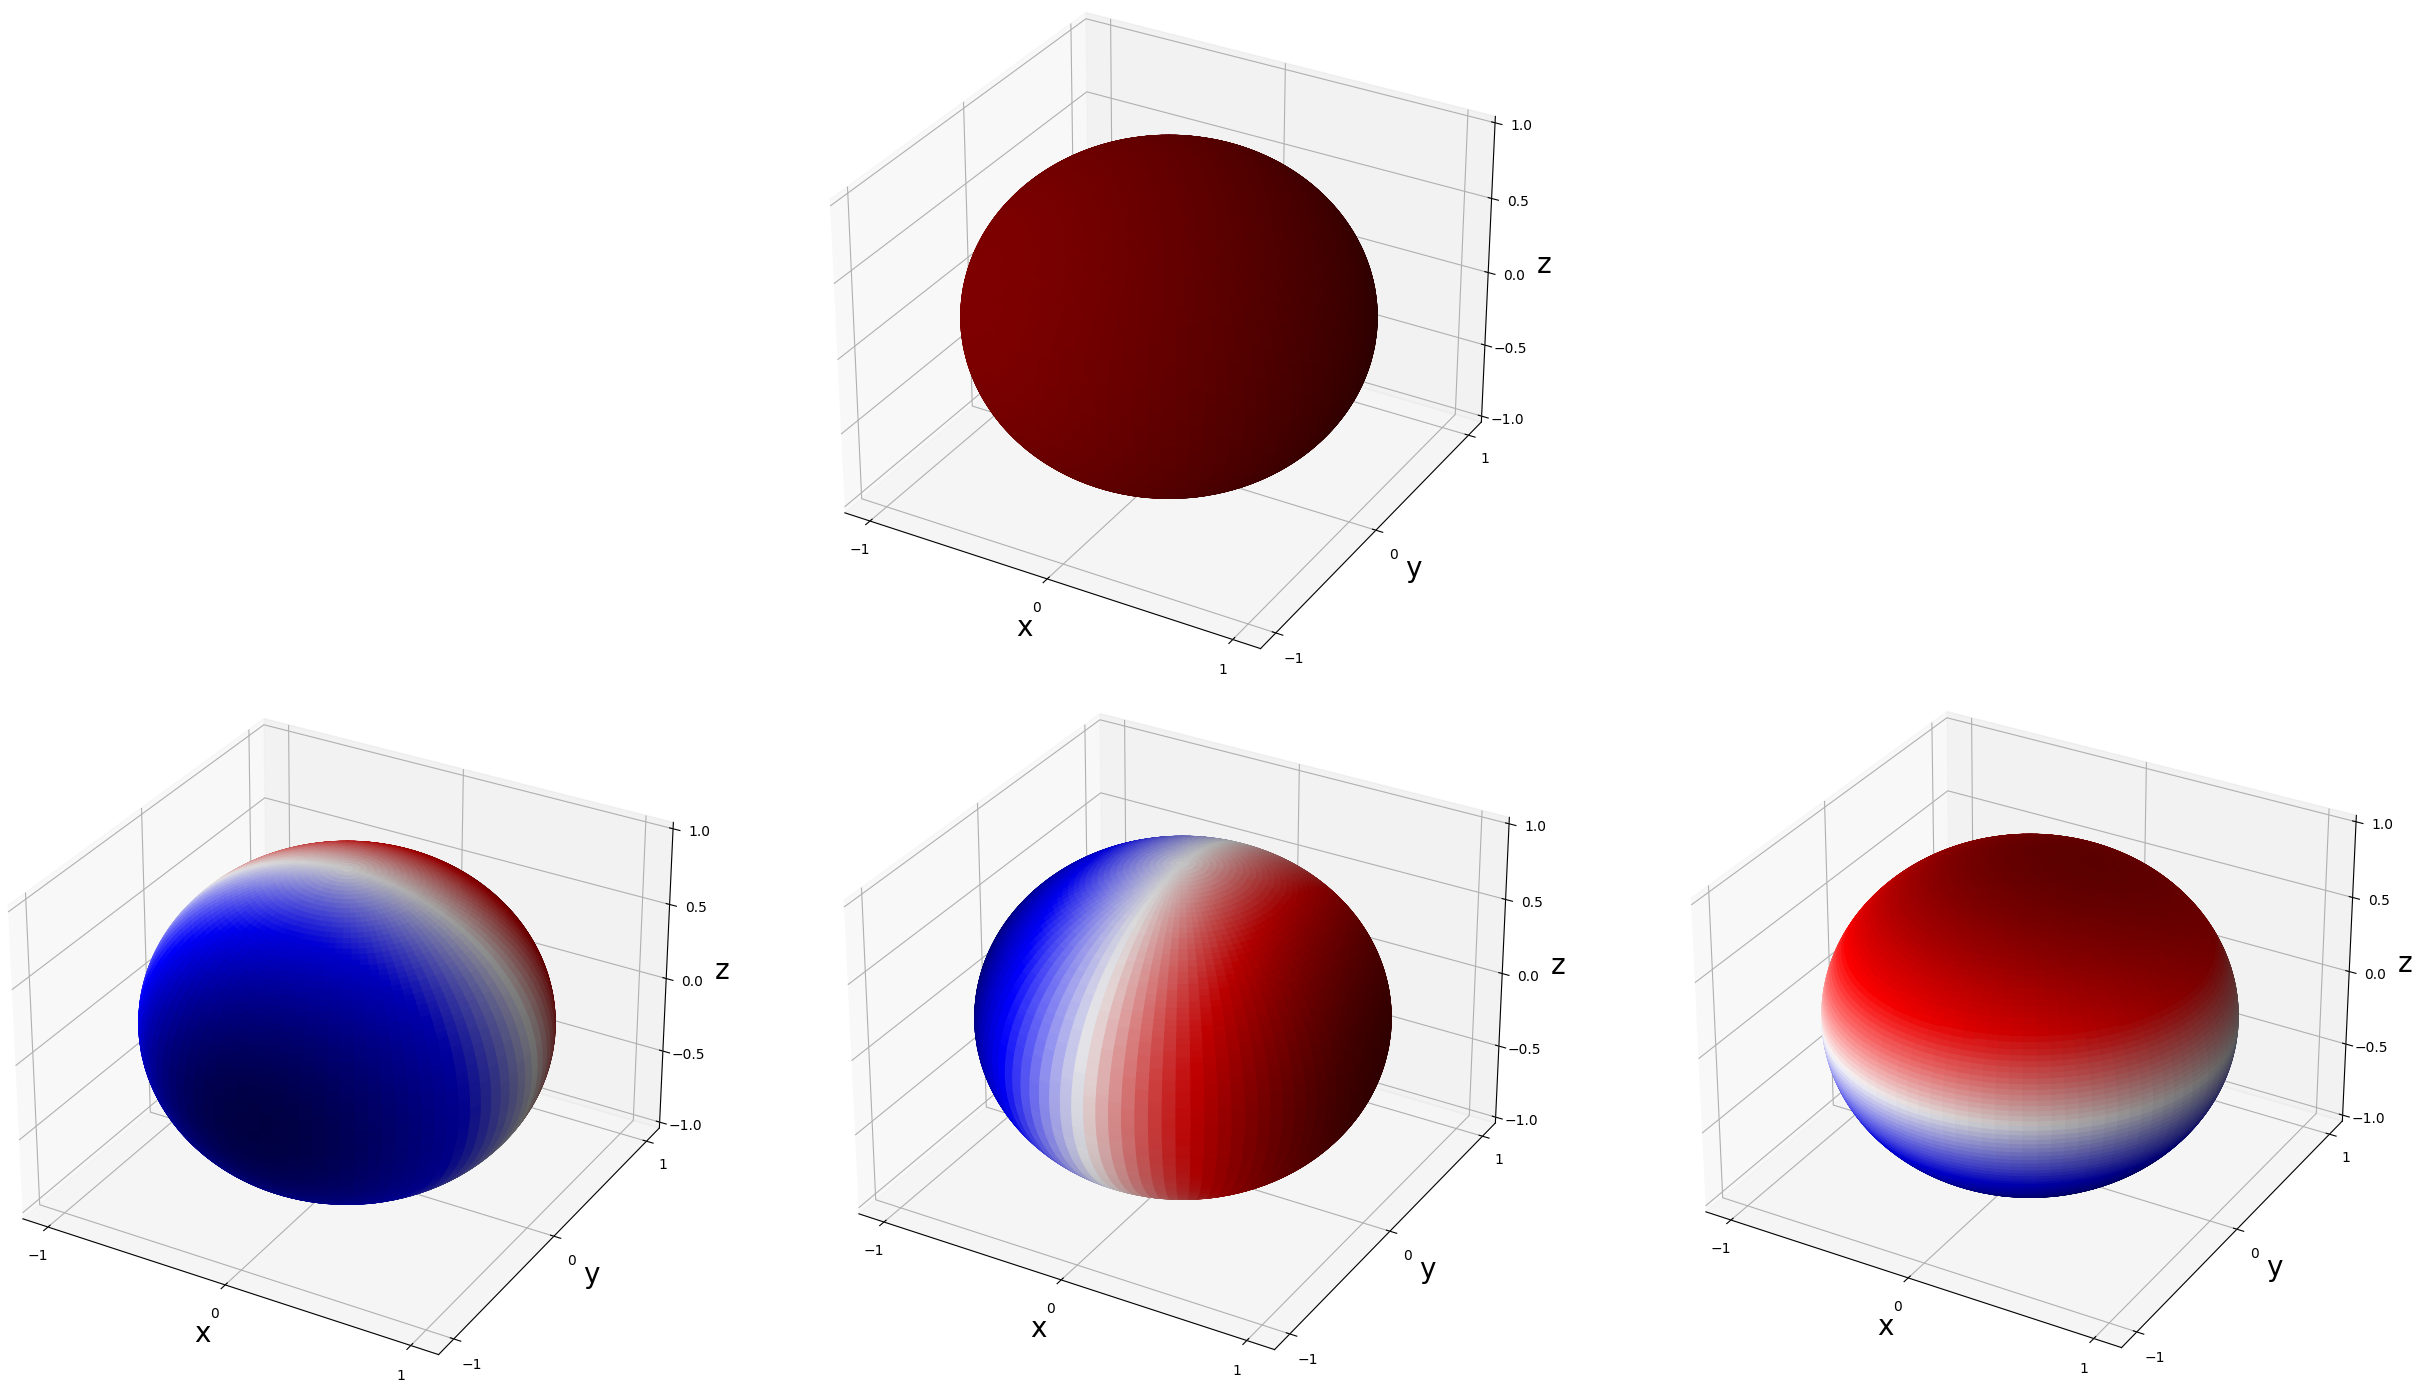
\includegraphics[width=1.\linewidth]{Images/chap2/foa.png}
    \captionof{figure}[First-order Ambisonics directivities]{First-order Ambisonics directivities. Top: $\tilde{Y}_0^0$ normalized, corresponding to $W$. Bottom, from left to right: $\tilde{Y}_1^1$, $\tilde{Y}_1^{-1}$, $\tilde{Y}_1^0$ normalized, corresponding to $X$, $Y$, $Z$, respectively. The red regions correspond to positive values and the blue regions correspond to negative values.}
    \label{fig:foa}
    \end{center}
\end{figure}

As a consequence of its low number of channels, which is a practical advantage here, the FOA format suffers from a low spatial resolution when representing the sound field \cite{rafaely_analysis_2005}. One consequence is the reduction of the \textit{sweet spot} size: it is the spatial region between the loudspeakers in which the restitution of the original sound field is the most accurate. 

Note that the Ambisonics format can be transposed directly into the short-time Fourier transform (STFT) domain, \emph{i.e.}, for each STFT time frame index $t$ and frequency bin $f$ \footnote{Note that in this thesis we use the notations $t$ and $f$ for the frame index and frequency bin in the STFT domain, as it is usually employed. Those notations are also used to express the physical frequency $f$ and time $t$ only for some preliminary discussions as in this chapter.}, we have:
\begin{equation}
\label{eq:foaSTFT}
\mathbf{x}(t,f) = 
\begin{bmatrix} W(t,f) \\ X(t,f) \\ Y(t,f) \\ Z(t,f) \end{bmatrix}
= \begin{bmatrix} 1 \\ \sqrt{3} \cos \theta_k \cos \phi_k \\ \sqrt{3} \sin \theta_k \cos \phi_k \\ \sqrt{3} \sin \phi_k \end{bmatrix} s(t,f).
\end{equation}

\subsection{Higher-order Ambisonics}

To improve the spatial resolution of the Ambisonics representation, we can increase the order $N$, leading to more components. When $N>1$, we call it the higher-order Ambisonics representation. For an order $N$, there are $(N+1)^2$ channels to represent the original signal. Table~\ref{tab:hoaComponents} sums up the directivities of the HOA components up to order 3, also illustrated in Fig~\ref{fig:hoa}. Using HOA components notably increases the size of the sweet spot and the resolution of the spatial characteristics of the encoded sound field, but at the cost of more channels to handle.

\begin{table}[h!]
\centering
\begin{tabular}{|cccc|}
\hline
$n$        & $m$ & \rule{0pt}{12pt} $\tilde{Y}_n^m$ & $\tilde{Y}_n^m(\theta,\phi)$ \\ \hline
   $0$               & \rule{0pt}{12pt} $0$           &  $\tilde{Y}_0^0$          & $1$           \\ \hline
\rule{0pt}{12pt}  & $-1$          &  $\tilde{Y}_1^{-1}$          & $\sqrt{3} \cos \theta \cos \phi$         \\
  $1$                &     \rule{0pt}{12pt} $0$      &   $\tilde{Y}_1^0$         &  $\sqrt{3} \sin \theta \cos \phi$    \\
                  &     \rule{0pt}{12pt}  $1$      &  $\tilde{Y}_1^1$          &       $\sqrt{3} \sin \phi$     \\ \hline
 & \rule{0pt}{14pt} $-2$        &  $\tilde{Y}_2^{-2}$          & $\frac{\sqrt{15}}{2} \sin 2 \theta \cos^2 \phi$           \\
                  &    \rule{0pt}{14pt} $-1$        &  $\tilde{Y}_2^{-1}$          &
                  $\frac{\sqrt{15}}{2} \sin \theta \sin 2 \phi$          \\
 $2$                 &  \rule{0pt}{14pt}   $0$       &  $\tilde{Y}_2^{0}$          &   $\frac{\sqrt{5}}{2} (3 \sin^2 \phi -1)$      \\
                  &   \rule{0pt}{14pt}  $1$       &  $\tilde{Y}_2^{1}$          &   $\frac{\sqrt{15}}{2} \cos \theta \sin 2 \phi$         \\
                  &   \rule{0pt}{14pt}  $2$       &  $\tilde{Y}_2^{2}$          &   $\frac{\sqrt{15}}{2} \cos 2 \theta \cos^2 \phi$         \\ \hline
 &  \rule{0pt}{14pt} $-3$            &  $\tilde{Y}_3^{-3}$          & $\sqrt{\frac{35}{8}} \sin 3 \theta \cos^3 \phi$            \\
                  & \rule{0pt}{14pt}  $-2$         &  $\tilde{Y}_3^{-2}$          & $\sqrt{\frac{105}{2}} \sin 2 \theta \sin \phi \cos^2 \phi$            \\
                  & \rule{0pt}{14pt} $-1$           &  $\tilde{Y}_3^{-1}$          & $\sqrt{\frac{21}{8}} \sin \theta \cos \phi (5\sin^2 \phi-1)$           \\
     $3$             &  \rule{0pt}{14pt} $0$         &  $\tilde{Y}_3^{0}$          &  $\frac{1}{2} \sin \phi (5 \sin^2 \phi -3)$          \\
                  &  \rule{0pt}{14pt}  $1$        &  $\tilde{Y}_3^{1}$          & $\sqrt{\frac{21}{8}} \cos \theta \cos \phi (5 \sin^2 \phi-1)$           \\
                  & \rule{0pt}{14pt} $2$           &  $\tilde{Y}_3^{2}$          & $\sqrt{\frac{105}{2}} \cos 2 \theta \sin \phi \cos^2 \phi$           \\
                  & \rule{0pt}{14pt} $3$           &  $\tilde{Y}_3^{3}$          & $\sqrt{\frac{35}{8}} \cos 3 \theta \cos^3 \phi$           \\ \hline
\end{tabular}
\caption[Directivities of HOA components]{Directivities of HOA components up to order 3, with the N3D normalization standard \cite{daniel_representation_2001}.}
\label{tab:hoaComponents}
\end{table}

\begin{figure}[t]
    \begin{center}
    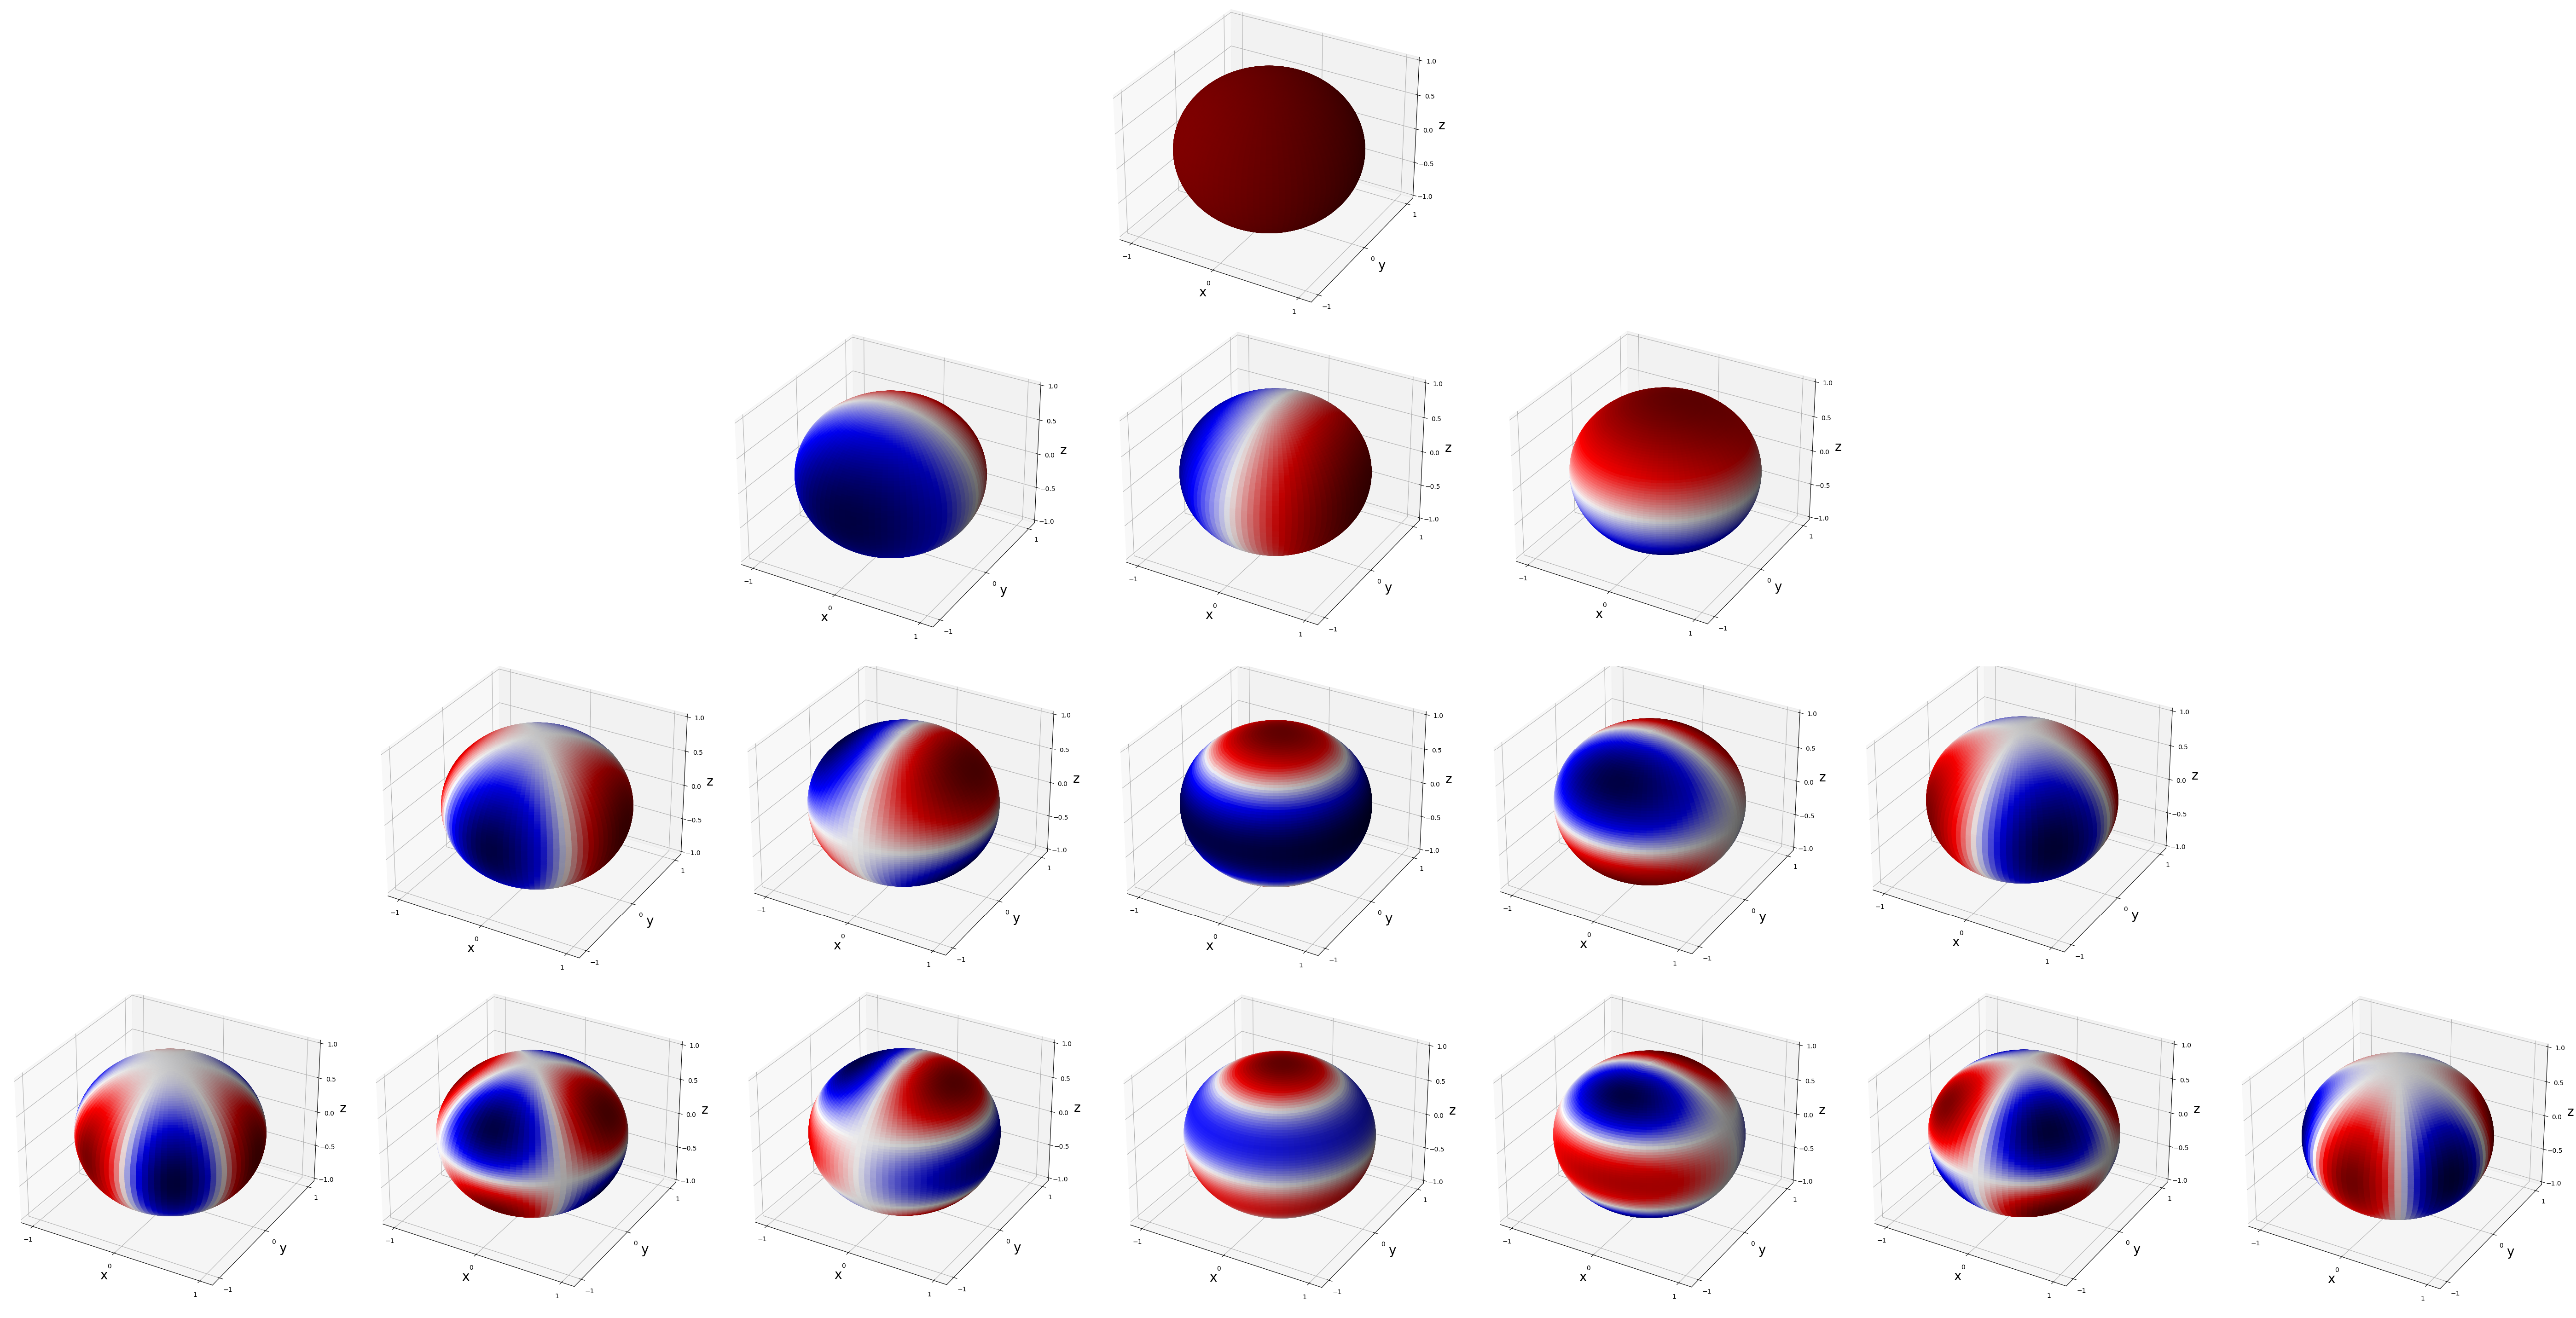
\includegraphics[width=1.\linewidth]{Images/chap2/hoa.png}
    \captionof{figure}[Higher-order Ambisonics directivities]{Higher-order Ambisonics directivities, with the spherical harmonics degree $n$ increasing from top to bottom and the order $m$ increasing from left to right. Red regions correspond to positive values and blue regions correspond to negative values.}
    \label{fig:hoa}
    \end{center}
\end{figure}


\subsection{Ambisonic encoding}
\label{subAmbEncoding}

In practice, Ambisonic signals (FOA or HOA respresentations) are computed from the finite number of acoustic pressure observations $\{p_i\}_{i\in[1,I]}$, measured by a microphone array. Denoting by $\mathbf{p} \in \mathbb{R}^I$ and $\mathbf{b} \in \mathbb{C}^{(N+1)^2}$ the vectors of concatenated observations $p(r,\theta_i,\phi_i,t)$, $i\in[1,I]$, and coefficients $B_n^m$, respectively, the expression~\eqref{eqAmbiDecomp} can be compactly written as
\begin{equation}
    \mathbf{p} \approx \mathbf{Y} \mathbf{W} \mathbf{b},
\end{equation}
where $\mathbf{Y} \in \mathbb{R}^{I \times (N+1)^2}$ is the matrix whose rows contain spherical harmonic functions $\tilde{Y}^m_n(\theta_k,\phi_k)$, evaluated at the directions $(\theta_i,\phi_i)$, and $\mathbf{W} \in \mathbb{C}^{(N+1)^2 \times (N+1)^2}$ is the diagonal weight matrix whose entries contain a sum of $i^n j_n(kr)$ and a regularization term \cite{nicol_sound_2010}. Without additional information, one would need a microphone array containing $I \geq (N+1)^2$ channels to obtain the coefficients $\mathbf{b}$ of the order $N$, which imposes practical limitation for the design of an Ambisonics microphone.

%-----------------------------------------------
%  INTENSITY, FDVV, TDVV
%-----------------------------------------------
\section{Sound intensity and velocity vector}

In the section~\ref{sec:ambisonics}, we introduced the definition of the Ambisonics coefficients, which are sufficient to entirely represent the sound field at any recording point. In this section, we present several representations based on the Ambisonics format which will be useful in the remainder of this thesis.

\subsection{Sound intensity vector}

\subsubsection{Definition}
\label{ss:pseudointensityVector}

Sound intensity is a fundamental acoustic quantity that is often used to characterize the distribution of energy of a sound field \cite{williams_fourier_2000}. Often expressed as a time-averaged quantity over certain temporal segment, it describes the magnitude and direction of the flow of sound energy per unit area \cite{jacobsen_fundamentals_2013}. For narrowband signals, one can define the complex ``steady state'' sound intensity vector as \cite{jacobsen_note_1991,williams_fourier_2000}:
\begin{equation}
\label{eq:intensityDefinition}
    \mathbf{I} = p \mathbf{u}^*,
\end{equation}
where $p$ is the sound pressure, $\mathbf{u}$ is the particle velocity vector, which is the physical velocity of the particles in motion which transmit the wave \cite{kinsler_fundamentals_2000}.

It can be shown that the sound pressure $p$ and the particle velocity vector $\mathbf{u}$ are related by the \textit{linearized fluid momentum equation} \cite[p.~27]{merimaa_analysis_2006}:
\begin{equation}
    - \nabla p = \rho_0 \frac{\partial \mathbf{u}}{\partial t},
\end{equation}
with $\nabla$ being the gradient operator and $\rho_0$ denoting the air density. 

The omnidirectional channel $W$ can be considered as an estimate of the acoustic pressure at the microphone position, while the FOA channels $X$, $Y$ and $Z$ approximate the spatial derivatives of pressure $p$ along the Cartesian coordinate axes \cite[p.~50]{merimaa_analysis_2006}. Therefore, one can approximate the particle velocity vector relatively to these channels with \cite[p.~90]{pulkki_parametric_2018} (the factor $1/\sqrt{3}$ is due to the presumed N3D normalization \cite{daniel_representation_2001}):
\begin{equation}
\label{eq:velocityVectorApprox}
\mathbf{u}(t) = - \frac{1}{\rho_0 c \sqrt{3}}
\begin{bmatrix} X(t) \\ Y(t) \\ Z(t) \end{bmatrix}.
\end{equation}
As we will see later, we are mainly interested in the \emph{direction} of the vector $\mathbf{u}(t)$, hence, by an abuse of notation, we also denote by $\mathbf{u}$ the normalized particle velocity vector. 

Since the previous equation is an approximation, injecting it into \eqref{eq:intensityDefinition} leads to an approximation of the intensity vector, which we call the \textit{pseudointensity} vector (PIV). To simplify the notation, we use the same symbol $\mathbf{I}$ to refer to the pseudointensity vector, which is now expressed using only the FOA components (in the STFT domain) as:
\begin{equation}
    \mathbf{I}(t,f) = \alpha \begin{bmatrix} W(t,f) X^*(t,f) \\ W(t,f) Y^*(t,f) \\ W(t,f) Z^*(t,f) \end{bmatrix},
\end{equation}
with $\alpha = - \frac{1}{\rho_0 c \sqrt{3}}$ a factor that will be dropped thereafter. As for the remaining of this thesis, we will refer to the pseudointensity vector based on FOA components as the \textit{first-order-pseudointensity vector} (FO-PIV).

\subsubsection{Active first-order-pseudointensity vector}

We define the \textit{active first-order-pseudointensity vector} as the real part of the complex FO-PIV:
\begin{equation}
    \label{eq:activeFOPIV}
    \mathbf{I}_a = \begin{bmatrix} \mathfrak{R}\big(W(t,f) X^*(t,f)\big) \\ \mathfrak{R}\big(W(t,f) Y^*(t,f)\big) \\ \mathfrak{R}\big(W(t,f) Z^*(t,f)\big) \end{bmatrix}.
\end{equation}
This quantity physically represents the transport of sound energy in the fluid, and it can be shown to be proportional to the gradient of the phase of sound pressure \cite{jacobsen_fundamentals_2013}. In other words, assuming free-field propagation, active intensity is orthogonal to the propagating wavefront.

\subsubsection{Reactive first-order-pseudointensity vector}

The \textit{reactive first-order-pseudointensity vector} is defined as the imaginary part of the complex FO-PIV:

\begin{equation}
\label{eq:reactiveFOPIV}
    \mathbf{I}_r = \begin{bmatrix} \mathfrak{I}\big(W(t,f) X^*(t,f)\big) \\ \mathfrak{I}\big(W(t,f) Y^*(t,f)\big) \\ \mathfrak{I}\big(W(t,f) Z^*(t,f)\big) \end{bmatrix}.
\end{equation}
Physically, the reactive FO-PIV represents the dissipative local energy transfers \cite{daniel_representation_2001}, and is orthogonal to the surfaces of equal energy of sound pressure \cite{jacobsen_fundamentals_2013,daniel_representation_2001}. While being negligible under the far/free field assumptions, reactive intensity becomes important in reverberant conditions.

\subsubsection{Higher-order pseudointensity vector}

We extend the previously introduced FO-PIV by using HOA components. The general expression for this \textit{higher-order-pseudointensity vector} (HO-PIV) is, at order $N$:
\begin{equation}
    \mathbf{I}^N(t,f) = B_0^0(t,f) \mathbf{B}_{1:N}^*(t,f),
\end{equation}
where $\mathbf{B}_{1:N}$ is the vector containing all HOA channels for $n=1$ to $N$ (there are $(N+1)^2-1$ channels in total). We can see that $\mathbf{I}^1$ corresponds to the FO-PIV. 

The definition of the active and reactive HO-PIV using HOA components ($\mathbf{I}^N_a$ and $\mathbf{I}^N_r$) is similar to the first-order case, \emph{i.e.}, they correspond to the real and imaginary part of the HO-PIV $\mathbf{I}^N$, respectively.

\subsubsection{Pseudointensity vector normalization}

A normalized version of the FO-PIV is obtained as follows:
\begin{equation}
     \bar{\mathbf{I}}(t,f) = \frac{\mathbf{I}(t,f)}{\lvert W(t,f) \rvert^2 + \frac{1}{3} \big(\lvert X(t,f) \rvert^2 + \lvert Y(t,f) \rvert^2 + \lvert Z(t,f) \rvert^2\big)}.
 \end{equation}
Note that the norm of $\bar{\mathbf{I}}(t,f)$ is upper bounded by $1$.

More generally, the normalized HO-PIV\footnote{Again, assuming the N3D normalization standard.} is given by:
\begin{equation}\label{eqHOpinv}
     \bar{\mathbf{I}}^N(t,f) = \frac{\mathbf{I}^N(t,f)}{\sum_{n=0}^N \frac{1}{2n+1} \sum_{m=-n}^n \lvert B_n^m \rvert ^2}.
\end{equation}

Assuming that the time-frequency bin $(t,f)$ is dominated by a single source, the normalized (FO-/HO-)PIV is independent of the source signal ``content'' $s(t,f)$, and mainly encodes the spatial footprint of sound propagation. This is easily observed for the plane wave propagation, since (according to \eqref{eqPlaneWaveCf}), we have $B_0^0 {B_n^m}^* \propto |B|^2$. The latter term cancels out in \eqref{eqHOpinv}, and the remaining part depends only on the corresponding spherical harmonics of different orders.

\subsection{Frequency-domain velocity vector}

The sound PIV was defined as the product between the first Ambisonics channel $W:=B_0^0$ and the other channels ($X$, $Y$ and $Z$ for FO-PIV, and all channels except $W$ for HO-PIV). We also showed a way to normalize the PIV to bound its values. A related representation, termed Frequency-Domain Velocity vector (FDVV) in  \cite{daniel_representation_2001}, is obtained by dividing the complex conjugate of FO-PIV by $\lvert W(t,f) \rvert ^2$:
\begin{equation}\label{eqFDVV}
    \mathbf{V}(t,f) = \frac{\mathbf{I}(t,f)^*}{\lvert W(t,f) \rvert ^2} = 
    \frac{1}{W(t,f)}
    \begin{bmatrix} X(t,f) \\ Y(t,f) \\ Z(t,f) \end{bmatrix}.
\end{equation}
Analogously to $\bar{\mathbf{I}}(t,f)$, due to the division by $\lvert W(t,f) \rvert ^2$, the FDVV has the advantage of being less dependent on the energy and therefore on the content of the signal. As for the complex PIV, we can separate the FDVV into the real and imaginary parts. 

\subsection{Time-domain velocity vector}
\label{ss:tdvv}

In this section, we will define the \textit{time-domain velocity vector} as the inverse Fourier transform (IFT) of the FDVV\footnote{Note that FDVV and TDVV are also known as \emph{Relative Transfer Function} and \emph{Relative Impulse Response} (in the spherical harmonic domain), respectively \cite{jarrett_theory_2017}.} \cite{daniel_time_2020}, but we modify the expression of the FDVV a bit beforehand.

We place ourselves in a single-source environment in which the Ambisonics recording captures the multipath signal. For a single timestep, due to the superposition principle \eqref{eqSRIR}, each recorded FOA channel will be a sum of delayed and attenuated copies of the source signal $s(t)$ (with an attenuation depending on the incoming wavefront direction and channel directivity). Under the far field assumption, the $n$\textsuperscript{th} such wavefront $\mathbf{x}_n(t)$ may be represented by a plane wave. According to \eqref{eqPlaneWave}, the FOA components of the plane wave propagating from the direction $(\theta_n,\phi_n)$, in frequency domain, are compactly expressed by
\begin{equation*}
    \mathbf{x}_n(f) = \left[ \begin{matrix} 1 \\ \sqrt{3} \mathbf{u}_n, \end{matrix} \right] s(f),
\end{equation*}
where $\mathbf{u}_n$ is the corresponding normalized particle velocity defined in \eqref{eq:velocityVectorApprox}.

The recorded signal, in the noiseless case, is then a sum of FOA-encoded plane waves:
\begin{equation*}
    \mathbf{x}(f) = s(f) \sum_{n} a_n(f) \mathbf{x}_n(f),
\end{equation*}
with $a_n(f)$ being the complex magnitude (incorporating both the common attenuation factor and phase shift) of the sound wave at frequency $f$.

Plugging these expressions into the definition of FDVV \eqref{eqFDVV}, we can now decompose the FDVV at frequency $f$ into the different reflections\footnote{Here we use the symbol ``$\simeq$'' instead of equality due to the N3D encoding factor $\sqrt{3}$ in the denominator. Without loss of generality, we drop this value in the ensuing expressions.}:
\begin{equation}
    \mathbf{V}(f) \simeq \frac{\sum_n a_n(f) \mathbf{u}_n}{\sum_n a_n(f)} = \frac{\mathbf{u}_0 + \sum_{n \geq 1} \gamma_n(f) \mathbf{u}_n}{1+\sum_{n \geq 1} \gamma_n(f)},
\end{equation}
where $\gamma_n(f) = \frac{a_n(f)}{a_0(f)} = g_n(f) e^{-2i \pi f \tau_n}$ is the relative \emph{gain} of the $n^{th}$ reflection with respect to the direct path (without losing generality we assume that $n$ follows the order of reflections).
Assuming that $\lvert \sum_{n \geq 1} \gamma_n(f) \rvert < 1$, we can express $\mathbf{V}(f)$ using the Taylor series of the function $f(x) = \frac{1}{1+x}$ :
\begin{equation}
    \mathbf{V}(f) = \Big(\mathbf{u}_0 + \sum_{n \geq 1} \gamma_n(f) \mathbf{u}_n \Big) \sum_{k=0}^{\infty} \Big( \sum_{n = 1}^{\infty} - \gamma_n(f) \Big)^k,
\end{equation}
which we can rearrange by separating the terms from the primary reflections and the terms coming from the interactions between reflections:
\begin{equation}
\begin{aligned}
        \mathbf{V}(f) &= \mathbf{u}_0 + \mathbf{u}_0 \sum_{k=1}^{\infty} \Big( \sum_{n=1}^{\infty} -g_n(f) e^{-2i \pi f \tau_n} \Big)^k \\
                      &+ \sum_{k=0}^{\infty} \sum_{n=1}^{\infty} \Big(g_n(f) e^{-2i \pi f \tau_n} \mathbf{u}_n \Big) \Big( \sum_{n=1}^{\infty} -g_n(f) e^{-2i \pi f \tau_n} \Big)^k \\
                      &= \mathbf{u}_0 + \mathbf{u}_0 \sum_{k=1}^{\infty} \sum_{n=1}^{\infty} \Big( -g_n(f) e^{-2i \pi f \tau_n} \Big)^k \\
                      &+ \sum_{k=0}^{\infty} \sum_{n=1}^{\infty} - \mathbf{u}_n  \Big( -g_n(f) e^{-2i \pi f \tau_n} \Big)^k + \Lambda(f),
\end{aligned}
\end{equation}
where $\Lambda(f)$ contains the cross terms of the interactions between reflections. Finally we obtain:
\begin{equation}
    \mathbf{V}(f) = \mathbf{u}_0 + \sum_{k=0}^{\infty} \sum_{n=1}^{\infty} \Big(\mathbf{u}_0 - \mathbf{u}_n \Big) \Big(-g_n(f)\Big)^k e^{-2i \pi f k \tau_n} + \Lambda(f).
\end{equation}

Assuming now that $g_n(f)=g_n$ is frequency-independent, we now apply the IFT of $\mathbf{V}$ to define the \textit{time-domain velocity vector} (TDVV) :
\begin{equation}
\label{eq:TDVVdefinition}
    \mathbf{V}(t) = \delta(t) \mathbf{u}_0 + \sum_{k=0}^{\infty} \sum_{n=1}^{\infty} \Big(\mathbf{u}_0 - \mathbf{u}_n\Big) (-g_n)^k \delta(t-k \tau_n) + \lambda(t),
\end{equation}
with $\delta$ denoting the Dirac delta function and $\lambda(t)$ the IFT of $\Lambda(f)$.

\begin{figure}[t]
    \begin{center}
    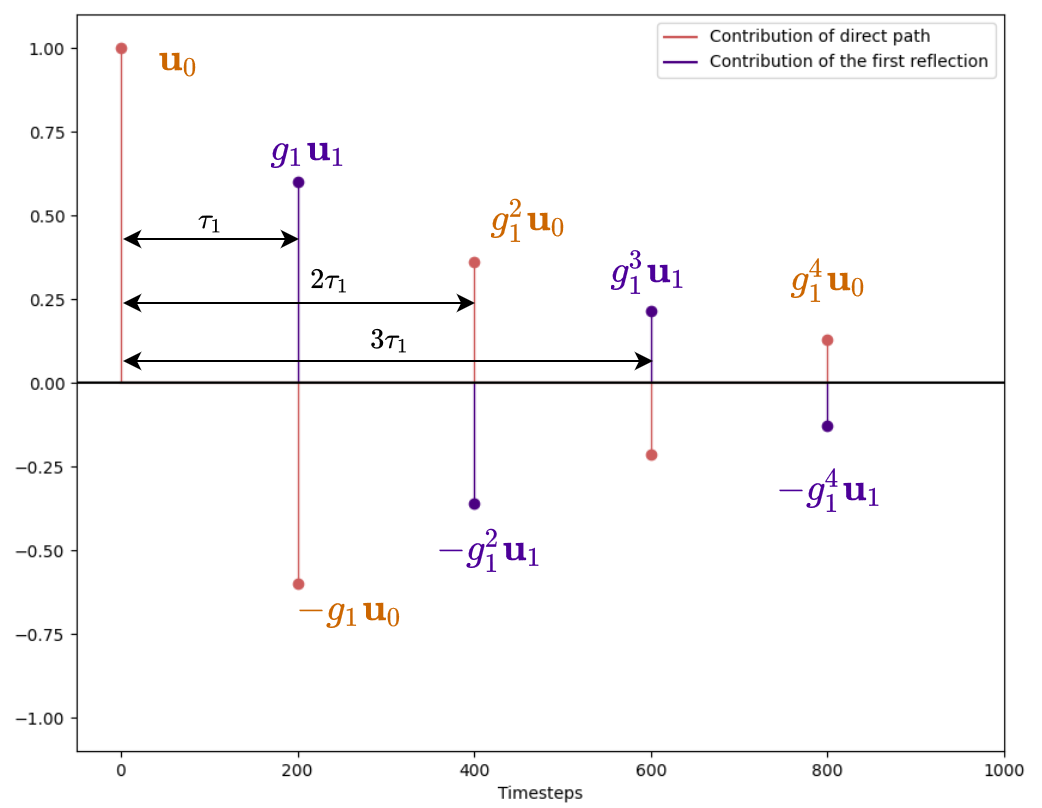
\includegraphics[width=0.8\linewidth]{Images/chap2/tdvv_1reflection_annote.png}
    \captionof{figure}[Theoretical time-domain velocity vector considering only one reflection]{Theoretical time-domain velocity vector considering only one reflection. The first orange peak at $t=0$ contains the coordinates of a vector colinear to the source DoA, representing the direct path between the source and the microphone array. The other orange peaks represent the contribution of the direct path to the value of the TDVV for different timesteps, while the purple peaks represent the contribution of the first reflection. All the peaks are equally spaced by an interval equal to $\tau_1$, and the peak amplitudes exponentially decay by a factor $-g_1$, with alternating sign.}
    \label{fig:TDVV_oneReflection}
    \end{center}
\end{figure}


In order to better appreciate the information contained in the TDVV, let us first assume that there is only one reflection in the considered environment:
\begin{equation}
    \mathbf{V}(t) = \delta(t) \mathbf{u}_0 + \sum_{k=0}^{\infty} \Big(\mathbf{u}_0 - \mathbf{u}_1\Big) (-g_1)^k \delta(t-k \tau_1) + \lambda(t).
\end{equation}
Fig.~\ref{fig:TDVV_oneReflection} illustrates what the TDVV looks like when considering only one reflection. As the TDVV is a vector with three coordinates (considering only the FOA domain), the coordinate in $y$-axis actually encodes the vector coordinates (the $x$-axis represents time). At $t=0$, we have $\mathbf{u}(0) = \mathbf{u}_0$ which is a vector colinear to the signal DoA. Then when $t$ increases we have a series of exponentially decaying peaks which are colinear to $\mathbf{u}_0 - \mathbf{u}_1$ at all time values which are multiples of $\tau_1$. Therefore we can theoretically retrieve the DoA, the first reflection direction, delay and relative gain with the TDVV under the assumptions of a single sound source with only one reflection and without noise.

\begin{figure}[t]
    \begin{center}
    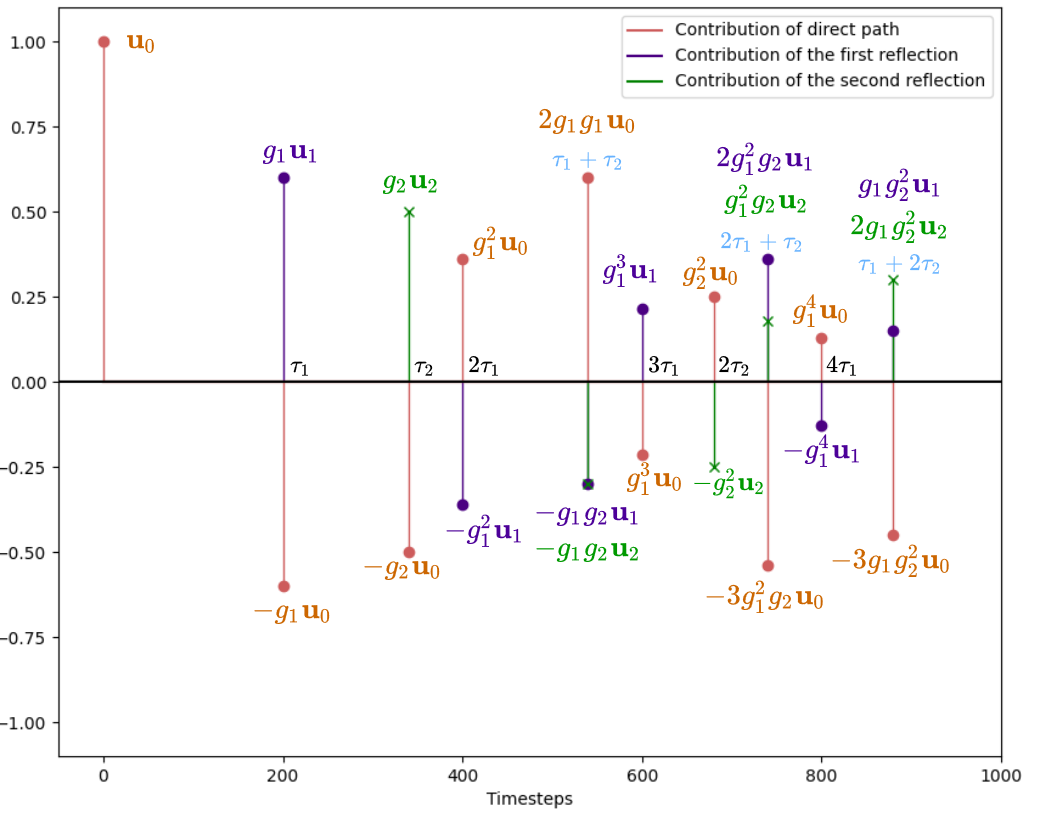
\includegraphics[width=0.8\linewidth]{Images/chap2/tdvv_2reflection_annote.png}
    \captionof{figure}[Theoretical time-domain velocity vector considering several reflections]{Theoretical time-domain velocity vector considering several reflections. The contributions of the direct path is represented in orange, those of the first reflection in purple and those of the second reflection in green. As in the case of only one reflection, the contributions corresponding to one reflection are equally spaced by $\tau_n$. In blue are indicated times for which the peaks contain the contributions of the interactions between the different reflections.}
    \label{fig:TDVV_twoReflections}
    \end{center}
\end{figure}

Now let us consider the general form of the TDVV with more than one reflection, leading to interaction between them. On Fig.~\ref{fig:TDVV_twoReflections} we can see what the TDVV looks like by illustrating the contributions of the direct path and the first two reflections, including the interactions (in blue in the figure). We can see that the peaks involving the contribution of only one of the reflections are still equally spaced by $\tau_n$. But now we see the appearance of some of the cross terms which were included in $\lambda(t)$ in \eqref{eq:TDVVdefinition}. Another phenomenon not represented in the figure can occur: theoretically, the different contributions of the reflections alone or those of the interaction between the reflections can overlap at the same time (related to the least common multiple of $\tau_n$) so it can be more difficult to separate the different contributions when analyzing the TDVV.

The TDVV thus provides an interesting representation to retrace the multipath propagation of a sound source. However, strong assumptions have been made to obtain an analytical expression for the TDVV: a single-source configuration without noise, frequency-independent gains, and the hypothesis that $\lvert \sum_{n \geq 1} \gamma_n(f) \rvert < 1, \forall f$ which is not fulfilled in practice. We do not push further the analysis of the TDVV in this thesis, since it is a relatively new idea in the literature. However, a certain number of experiments, discussed in Chapter~\ref{chap:tdvv}, has been conducted to exploit such a representation.


%-----------------------------------------------
%  CONCLUSION
%-----------------------------------------------
\section{Conclusion}

In this chapter, we introduced the framework we relied on in this thesis, based on the Ambisonics format. The main advantage of Ambisonics lies in the fact that it is capable of encoding a sound scene independently of the microphone array configuration, and without emphasizing any particular direction. We have shown the definition of the Ambisonics coefficients based on the spherical harmonics decomposition of the signal, which emerged from solving the wave equation in the spherical domain. These coefficients, considered at order $1$ (FOA) or higher (HOA), have been employed to define several physical quantities such as the FO- and HO-PIV, and the frequency-domain or time-domain velocity vector. All these sound representations have been used in our thesis work, generally as an input feature for neural networks, which are introduced in the next chapter.

\chapter{Artificial neural networks}
\label{chap:neuralNetworks}

\lettrine{A}{rtificial} neural networks (ANN) are a set of algorithms inspired by biological neural networks. They are the core components of deep learning \cite{goodfellow_deep_2016}, which itself can be defined as a part of machine learning. Machine learning refers to the capabilities of certain systems to learn how to perform a specific task, having been provided with an appropriate data for training. At the time of this thesis writing, in 2021, more and more applications have proven how much deep learning has improved the performance of machines in many various tasks, \emph{e.g.}, in image recognition \cite{he_deep_2016}, machine translation \cite{vaswani_attention_2017}, speech recognition \cite{hinton_deep_2012}, sound source separation \cite{hennequin_spleeter_2020}, board game playing \cite{silver_mastering_2017}, protein structure prediction \cite{jumper_highly_2021}, or music generation \cite{hadjeres_deepbach_2017}. While it has been shown that any task can be learned with a three-layer neural network \cite{hornik_multilayer_1989}, neural systems generally consist of many layers connected together, resulting in deep neural architectures, hence the term \textit{deep learning}. 

Many neural network architectures have been proposed in the past, and many of them were initially designed for a specific task, \emph{e.g.}, convolutional neural networks (CNN) for image recognition \cite{lecun_backpropagation_1989} or attention mechanism for machine translation \cite{he_deep_2016}. Due to their success, it is common to encounter adaptations of these architectures to address problems other than the original ones: for example, CNNs have been widely used for audio related tasks \cite{purwins_deep_2019}, while attention-based neural networks are commonly applied for computer vision \cite{dosovitskiy_image_2021}.

In this chapter, we provide a short overview of deep learning, and more precisely of different types of neural networks which were used throughout this thesis. Although the exploitation of artificial neural networks (ANN) is relatively new in the SSL literature (see Section~\ref{sec:SSLliterature}), deep learning is widely established in the audio research community, so this section is written assuming that the reader has some basic background on ANNs. We describe the different neural network architectures and mechanisms we exploited in this thesis. We assume this short introduction will be sufficient to help the reader to easily follow the experiments described in the next chapters. If needed, more in-depth description of deep learning can be found in \cite{goodfellow_deep_2016}. 

This chapter is organized as follows. Section~\ref{sec:mlp} introduces the basics of ANNs and the multilayer perceptron. Section~\ref{sec:cnn} explains the inner workings of a CNN, while Section~\ref{ss:recurrentNeuralNetworks} deals with recurrent neural networks (RNNs). Section~\ref{ss:residualNetworks} proposes a quick summary of residual connections. Finally, Section~\ref{sec:attentionMechanisms} describes the attention mechanism.

%-----------------------------------------------
%  MULTILAYER PERCEPTRON
%-----------------------------------------------
\section{Multilayer perceptron and backpropagation algorithm}
\label{sec:mlp}

\subsection{Multilayer perceptron or feedforward neural network}

A \textit{multilayer perceptron} (MLP) is a particular kind of artificial neural network in which all the connections are made forward, hence its name. In this section, we describe how an MLP can approximate a function using layers of artificial neurons and activation functions. We also explain how such a neural network can be trained with the backpropagation algorithm, with a review of loss functions and output units used throughout this thesis.

\subsubsection{Artificial neurons}

The fundations of artificial neural networks have been proposed as early as 1943 when McCulloch and Pitts \cite{mcculloch_logicial_1943} established a computational model of biological neurons. An artificial neuron is the building block of an ANN, and is composed of two stages :
\begin{itemize}
    \item A linear combination of its entries, using a set of weights specific to this neuron, as in \eqref{eq:artificialNeuron}
    \item The addition of a bias $b$
    \item An activation function $\sigma$ applied after the linear combination
\end{itemize}
\begin{equation}
\label{eq:artificialNeuron}
    y = \sigma \Big( \sum_{i=1}^{I} \theta_i x_i + b \Big),
\end{equation}
where $\{\theta_i\}_i$ and $b$ form the parameters of the neuron, $x_i$ are the entries of the input $\mathbf{x}$ and $y$ is the (scalar) output. We often set $b=\theta_0$ and append $1$ to the input vector so that $\{\theta_i\}_i$ is the entire set of weights.

Generally, multiple neurons are assembled to form a \textit{layer}, in which all the neurons are input with the same vector $\mathbf{x}$, thus each neuron of the same layer contains the same number of weights. An \textit{artificial neural network} is then defined to be a succession of $H$ layers of artificial neurons ($H$ is known as the \textit{depth} of the network), each layer being fed with the vector formed by the output of all neurons from the previous layer. If the layer $h$ is composed of $I_h$ neurons with input $\mathbf{x}^{h-1}$ (with $I_{h-1}$ components), then the entries of the output vector $\mathbf{x}^h$ are:
\begin{equation}
\label{eq:layerOutput}
    x_j^h = \sigma \bigg( \sum_{i=1}^{I_{h-1}} \theta_{j,i}^h x_i^{h-1} + b_j^h \bigg),
\end{equation}
for all $j \in \{1, ..., I_h\}$. This type of layer is called a \textit{fully-connected} layer or a \textit{feedforward} (FF) layer. The layer at $h=1$ is known as the \textit{input} layer, which directly receives the input features to its entries, and the last layer at $h=H$ is known as the \textit{output} layer. We generally name the output vector $\mathbf{y}$. The other layers are termed \textit{hidden} layers. 

We can rewrite \eqref{eq:layerOutput} in a more compact manner as:
\begin{equation}
\label{eq:layerOutputVectorized}
    \mathbf{x}^h = \sigma(\mathbf{b}^h + \mathbf{W}^h \mathbf{x}^{h-1}),
\end{equation}
where $\mathbf{b}^h$ is the \textit{bias} vector of layer $h$ and $\mathbf{W}^h$ is the weight matrix in $\mathbb{R}^{I_h \times I_{h-1}}$. This computation is known as a \textit{forward pass}.

The universal approximation theorem \cite{hornik_multilayer_1989} states that a MLP with two layers and a non-polynomial activation function at the first layer can approximate any function $f$ with an arbitrary accuracy.

\subsubsection{Activation functions}

There is a number of non-polynomial activation functions commonly used in the DL literature, as well as in this thesis. Linear activation functions are mostly used at the output layer, when the network is used in regression mode (see Section~\ref{ss:outputScheme}).

The \textit{rectified linear unit} (ReLU) is one of the most used activation function:
\begin{equation}
    \sigma(x) = max(0,x), \quad \forall x \in \mathbb{R}.
\end{equation}
This function has the advantage to preserving some of the properties that make linear models generalize well \cite{goodfellow_deep_2016}. 

The \textit{sigmoid} function is defined by:
\begin{equation}
    \sigma(x) = \frac{1}{1+e^{-x}}, \quad \forall x \in \mathbb{R}.
\end{equation}
Its values are always in $[0,1]$, and it converts large negative values to $0$ and large positive values to $1$. It is often used as an output activation function with its output value seen as a probability, which is particularly suitable for binary classification problems. Sometimes, the \textit{hard sigmoid} is preferred for its sharper contour:
\begin{equation}
    \sigma(x) = max\Big(0,min\big(1,\frac{x+1}{2}\big)\Big), \quad \forall x \in \mathbb{R}.
\end{equation}
The \textit{hyperbolic tangent (tanh)} function is defined by:
\begin{equation}
    \sigma(x) = \frac{e^{2x}-1}{e^{2x}+1}, \quad \forall x \in \mathbb{R}.
\end{equation}
The shape of tanh ressembles the shape of the sigmoid but it takes values within $[-1,1]$. Finally, the \textit{softmax} function is a generalization of the sigmoid function and produces a set of values within $[0,1]$:
\begin{equation}
    \sigma(y_i) = \frac{e^{x_i}}{\sum_{i=0}^{I} e^{x_i}},
\end{equation}
where $x_i$ and $y_i$ are the components of vectors $\mathbf{x}$ and $\mathbf{y}$, respectively. This function ensures that $\mathbf{y}$ can be seen as a probability distribution since its entries sum to $1$, which is particularly suitable for multi-class classification problems.


\subsection{The backpropagation algorithm}
\label{sec:backpropagationAlgorithm}

During the training stage, a neural network can adjust its weights with an algorithm called \textit{backpropagation} -- other algorithms exist - each time it is fed with a training example. To do that, the neural network performs a forward pass with training example $\mathbf{x}$, which gives an output value $\hat{\mathbf{y}}$. After choosing a \textit{loss} (or \textit{cost}) function $\mathcal{L}$, the knowledge of the target value $\mathbf{y}$ (which is known as the \textit{label} or \textit{ground-truth} of data $\mathbf{x}$) leads to the computation of the error made by the neural network for input $\mathbf{x}$, $\mathcal{L}(\mathbf{y},\hat{\mathbf{y}})$. The backpropagation algorithm uses this value $\mathcal{L}(\mathbf{y},\hat{\mathbf{y}})$ to adjust the weights of the neurons with a gradient descent. If at iteration $t$ of the backpropagation algorithm the weights are $\mathbf{w}^t$ (we drop the index $h$ for better visualization), the new value $\mathbf{w}^{t+1}$ at iteration $t+1$ is:
\begin{equation}
    \mathbf{w}^{t+1} = \mathbf{w}^{t} - \eta \frac{\partial \mathcal{L}(\mathbf{y}, \hat{\mathbf{y}})}{\partial \mathbf{w}^{t}},
\end{equation}
where $\eta$ is known as the \textit{learning rate}. This operation is done for all weights and for all training examples, by the means of training batches (composed of a certain numbers of these training examples), until some convergence criterion is met. In practice, the neural network is fed with the whole training set (each training pass using the whole training set is called an \textit{epoch}) for a certain number of times.

\subsubsection{Loss functions}

The choice for the loss function $\mathcal{L}$ depends on the output strategy employed to learn the considered task. The idea is to opt for a function that penalizes the difference between the ground-truth $\mathbf{y}$ and the estimated value $\hat{\mathbf{y}}$ with a sufficiently large value so that the change in weights due to gradient descent is significant. Moreover, loss functions are generally applied ``simultaneously'' on subsets of training examples called \textit{training batches}. In the following, we define the loss functions only for one training example, while for training batches the loss is obtained by summing the losses of all batch examples. Throughout this thesis, several loss functions were exploited:
\begin{itemize}
    \item Mean squared error (MSE) : $\mathcal{L}(\mathbf{y},\hat{\mathbf{y}}) =  \frac{1}{I} \sum_i^I (y_i - \hat{y}_i)^2$. When computing the loss for a training batch, the sum of all losses is divided by the number of examples in the batch, hence the term \textit{mean}. It is often used with a regression paradigm.
    
    \item Categorical cross-entropy : $\mathcal{L}(\mathbf{y},\hat{\mathbf{y}}) = - \sum_{i=1}^I y_i log(\hat{y}_i)$. This cross-entropy can be used for a classification problem, for which $\mathbf{y}$ is a one-hot vector (all entries are set to 0 except the one corresponding to the class which is set to 1). The softmax activation function suits well to this loss function.
    
    \item Binary cross-entropy : $\mathcal{L}(y,\hat{y}) = - y log(\hat{y}) + (1-y) log(\hat{y})$, which a particular case of the categorical cross-entropy when $I=1$, \emph{i.e.} the output is a scalar. It is generally used when $\mathbf{y}$ has a binary value ($0$ or $1$) and in conjonction with the sigmoid function which bounds the values of $\hat{\mathbf{y}}$ in $[0,1]$. If $\mathbf{y}$ and $\hat{\mathbf{y}}$ are vectors with binary values, the loss is obtained by summing the binary cross-entropy for each vector entry.
    
\end{itemize}

\subsection{Avoiding overfitting}

A major problem in neural networks is that the model can lack generalization when it is applied on data unseen during the training stage. This phenomenon is called overfitting, and part of deep learning research has been dedicated to avoid it and make the neural network to generalize better on unseen data. One strategy to control the learning of a neural network is to make use of a \textit{validation} dataset, which does not contain common data with the training dataset. During the training phase, the performance of the neural network is evaluated on the validation dataset (hence unseen data), and the training is stopped when the performance starts decreasing, meaning that the model starts overfitting on the training data. This monitoring method is known as \textit{early stopping}.

Another common regularization method is \textit{dropout} \cite{srivastava_dropout_2014}. It relies on bypassing random neurons (except for those in the output layer) based on a user-adjustable probability so that the output of these neurons are fixed to zero. This enforces the neural network not to overuse some specific neurons, and consequently prevents overfitting. This technique is employed only during training. Finally, batch normalization is a technique which can make a neural network more stable by rescaling and recentering the data in-between layers.

These methods were regularly used all along the experiments in this thesis.

%-----------------------------------------------
%  CONVOLUTIONAL NEURAL NETWORKS
%-----------------------------------------------
\section{Convolutional neural networks}
\label{sec:cnn}

Convolutional neural networks (CNN) are neural networks including convolutional layers which are specifically well-designed for processing data presented as a grid, for instance images represented by pixels. It has been pioneered in the end of the 1980s by LeCun et al. \cite{lecun_backpropagation_1989} to recognize handwritten digits in images. Since then, other new ideas around convolutional layers have been proposed in the literature. This section aims to provide a quick overview of CNNs, since they were used in our experiments.

\subsection{Convolutional layers}

As its name indicates, a convolutional layer applies convolutions on its input to produce an output, using a series of convolution kernels (or filters) $k$ which contain the learnable weights. In the 1D discrete domain (\emph{e.g.}, discrete time), this convolution is expressed by:
\begin{equation}
    y(n) = (x * k)(n) = \sum_i x(n-i)k(i),
\end{equation}
where $x$ and $y$ are the input and output, respectively, and $n$ is the discrete sample index. In practice, the kernel $k$ is a vector with a fixed size, so the sum is in a finite corresponding range. 

In the 2D domain, the convolution is applied in both dimensions:
\begin{equation}
    y(m,n) = (x * k)(m,n) = \sum_i \sum_j x(m-i,m-j) k(m,n).
\end{equation}
In this case, the kernel is a 2D matrix, and the same consideration applies regarding the range of the summation. Fig.~\ref{fig:2DconvolutionKernel} illustrates how a single 2D kernel of size $3 \times 3$ would be applied for each pixel of an input image.

\begin{figure}[t]
    \begin{center}
    \includegraphics[width=1.\linewidth]{Images/chap3/2DConvolutionKernel.png}
    \captionof{figure}[2D convolution operation with a $3 \times 3$ kernel]{2D convolution operation with a $3 \times 3$ kernel. Each $3 \times 3$ region on the image is multiplied with the kernel (right matrix), which is a 2D convolution operation, resulting in a scalar value associated to the region in the output. Zero-padding can optionally be used for regions on the edges. Note that the illustrated kernel is an example of how we can detect vertical contours with convolutions.}
    \label{fig:2DconvolutionKernel}
    \end{center}
\end{figure}

This convolution operation has also been extended to higher dimension, but this will be not used in this thesis. Zero-padding, \emph{i.e.}, automatic completion of input image edges with zeros, can be used  so that the output dimension is exactly the same as the input dimension. In contrast, one can use a \textit{stride}, \emph{i.e.}, a shift of the kernel operator in between two successive convolutions, greater than one so as to limit the size of the output and somehow ``compress'' the data representation, at the price of lower resolution.

During the training phase, the kernel matrix is learnt so that it provides the most meaningful convolution operation for the neural network to perform a task. In a convolutional layer, a bank of (possibly many) different  kernels are generally instantiated, so that each one can perform a specific operation, leading to different higher-level outputs, which are commonly called \textit{feature maps}. These outputs are then stacked, as illustrated in Fig.~\ref{fig:stackedConvolutionKernels}, and can become the input for another convolutional layer. 

\begin{figure}[t]
    \begin{center}
    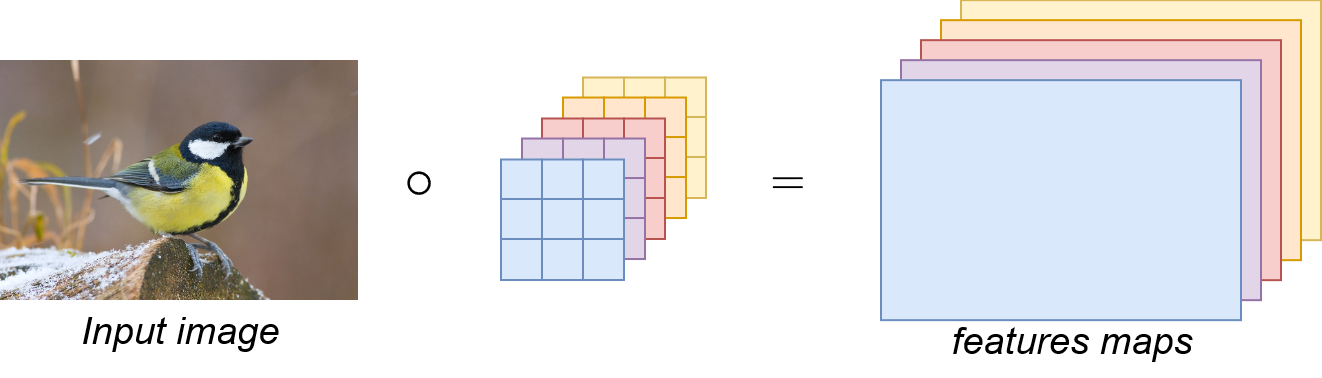
\includegraphics[width=1.\linewidth]{Images/chap3/stackedConvolutionKernels.png}
    \captionof{figure}[Application of multiple convolution kernels on a input image]{Application of multiple convolution kernels on a input image. Each kernel has its own set of learnable weights, and results in specific outputs, which are stacked in what is called feature maps.}
    \label{fig:stackedConvolutionKernels}
    \end{center}
\end{figure}

One major advantage of convolutional layers is that the operations are translation equivariant \cite{bronstein_geometric_2021}. In that way, each kernel can be learnt to highlight specific contours in the input feature, which is why several kernels are assembled in each convolutional layer. The obtained feature maps provide a somehow higher-level representation of the input signal, and stacking several convolutional layers one after another is often employed to perform \textit{feature extractions} in practice.

\subsection{Dilated convolutions}

A generalization of the convolution kernels presented above has been proposed in \cite{yu_multi-scale_2016}, under the name \textit{dilated convolution}. The idea is to apply the kernel on a downsampled version of the data, so that the convolution operation span is increased while keeping the same amount of learnable weights. This dilated convolution can be expressed by \cite{yu_multi-scale_2016}:
\begin{equation}
    (x * k)(n) = \sum_{i} x(n-li)k(i),
\end{equation}
where $l$ is the \textit{dilation factor}. For $l=1$, this operation is equivalent to the classical convolution. The idea can be extended to higher dimensions. Fig.~\ref{fig:dilatedConvolutions} illustrates how these dilated convolutions operate on input data, showing how it increases the convolution operation span. Dilated convolutions are also called \textit{atrous} convolutions, since we can see them as classical kernels with zeros inserted in between the actual weights.

\begin{figure}[t]
    \begin{center}
    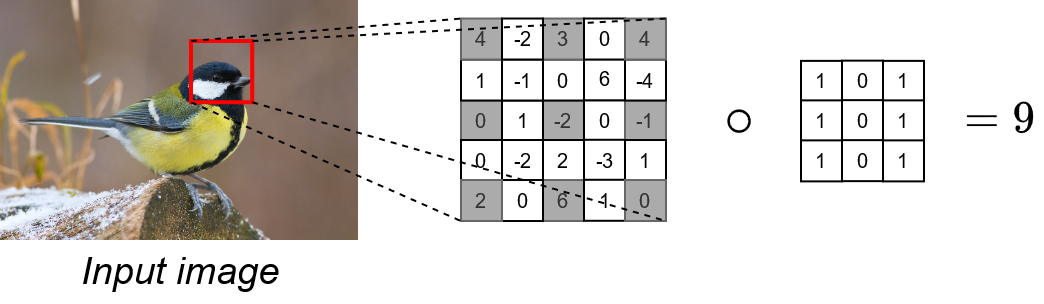
\includegraphics[width=1.\linewidth]{Images/chap3/dilatedConvolutions.png}
    \captionof{figure}[Visualization of dilated convolutions]{Visualization of dilated convolutions with a dilation factor $l=2$.}
    \label{fig:dilatedConvolutions}
    \end{center}
\end{figure}

\subsection{Pooling operation}

Pooling layers are also very common when using convolutional layers in neural networks. The goal of these layers is to downsample the data to reduce its dimensionality. The pooling size indicates the region shape in which only one value is extracted. If max-pooling is used, the highest value is kept, while if average pooling is used, the extracted value is the mean of all values in the corresponding region. As with convolutional layers, one can opt for a stride value, \emph{i.e.}, a shift that will skip data when applying the pooling operation. Fig.~\ref{fig:maxPooling} illustrates the max-pooling operation with a pooling size of $2 \times 2$ and a stride of $2$.

\begin{figure}[t]
    \begin{center}
    \includegraphics[width=0.6\linewidth]{Images/chap3/maxPooling.png}
    \captionof{figure}[Max-pooling operation]{Max-pooling operation. The operation is downsampling the data by keeping only the highest value of a considered region., In this example, the pooling size is $2 \times 2$ and the stride is $2$.}
    \label{fig:maxPooling}
    \end{center}
\end{figure}

%-----------------------------------------------
%   RECURRENT NEURAL NETWORKS
%-----------------------------------------------
\section{Recurrent neural networks}
\label{ss:recurrentNeuralNetworks}

Recurrent neural networks (RNN) are a family of neural networks that are suitable for processing sequential data, in which the ordering of successive data vectors bears importance. With MLPs or CNNs, data are processed one layer after another, without memorizing the operations within the network. The idea behind RNNs is to keep in memory some values (called \textit{states}) that contain a summary of past data information and which are used for further computation of the present output vector.

\subsection{Basic recurrent neural networks}

We consider a sequence of data vectors $\mathbf{x}^t$ where $t \in \{1,..., T\}$ is analog to a time index (although it could be any sequential index). In a basic recurrent layer, at each timestep $t$, a hidden vector $\mathbf{h}^t$ is considered in addition to the input vector $\mathbf{x}^t$. First, the hidden vector $\mathbf{h}^t$ is computed from the previous hidden vector $\mathbf{h}^{t-1}$ and the current input vector $\mathbf{x}^t$:
\begin{equation}
    \mathbf{h}^t = \sigma_h(\mathbf{W}_h \mathbf{h}^{t-1} + \mathbf{W}_x \mathbf{x}^t + \mathbf{b}),
\end{equation}
where $\mathbf{W}_h$ and $\mathbf{W}_x$ are weight matrices and $\mathbf{b}$ is the bias weight vector. Then, the output vector is computed as :
\begin{equation}
    \mathbf{y}^t = \sigma_y(\mathbf{W}_y \mathbf{h}^t),
\end{equation}
with $\mathbf{W}_y$ being the layer output weight matrix. Note that the activation functions $\sigma_h$ and $\sigma_y$ are not necessarily the same.
Fig.~\ref{fig:basicRecurrentLayer} illustrates how a basic recurrent layer processes data.

\begin{figure}[t]
    \begin{center}
    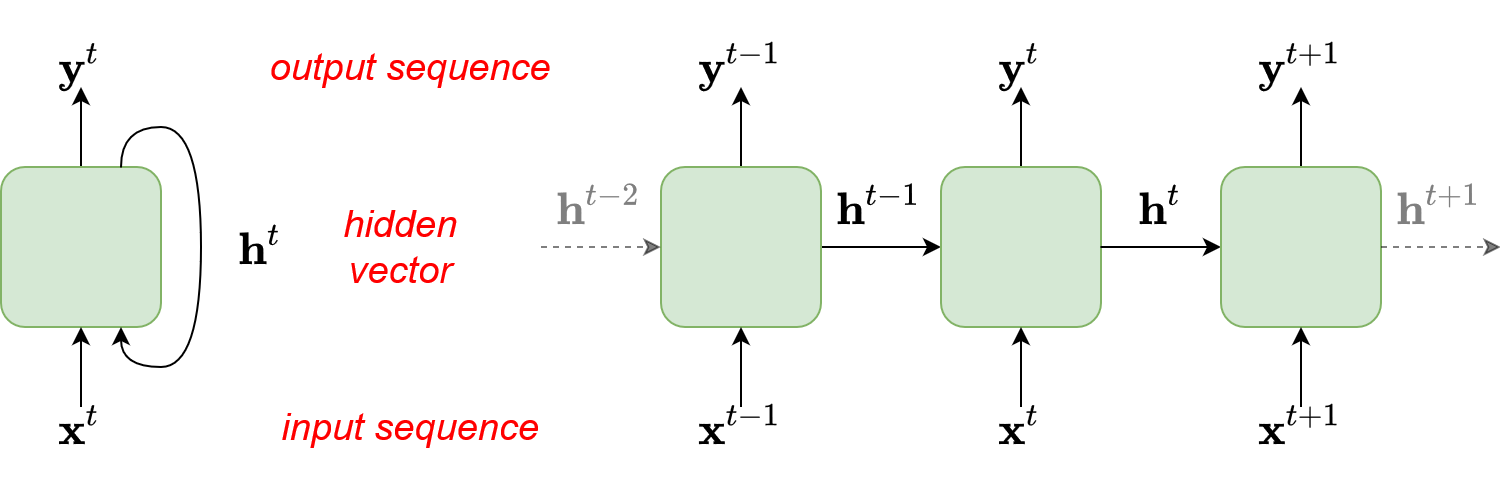
\includegraphics[width=1.\linewidth]{Images/chap3/basicRecurrentLayer.png}
    \captionof{figure}[Compact and unrolled visualization of a basic recurrent layer]{Compact (left) and unrolled (right) visualization of a basic recurrent layer.}
    \label{fig:basicRecurrentLayer}
    \end{center}
\end{figure}

Note that recurrent layers are often employed besides convolutional layers to form a convolutional recurrent neural network (CRNN).

\subsection{Backpropagation through time and vanishing gradient}

With the way a recurrent neural network is defined, one has to turn the usual backpropagation algorithm presented in Section~\ref{sec:backpropagationAlgorithm} into what is referred as backpropagation through time (BPTT). Without giving all details which can be found, \emph{e.g.}, in \cite{goodfellow_deep_2016}, the idea is to unfold the recurrent layer and consider the weights to be shared by each step. BPTT first relies on computing the loss for all timesteps of all sequences in the training batch. Then the gradient of the total loss for a specific weight is obtained as the sum of the gradients for each timestep. However the gradients for timesteps $t>0$ depends on the gradients for previous timesteps $t'<t$, so one needs to iterate backwards through time in order to compute all the gradients (hence the name BPTT).

One well-known limitation of this algorithm is the so-called \textit{vanishing gradient problem}. As the gradients are computed in an iterative way, some gradient values can become very small thus preventing the weight from changing its value. The more iterations are considered the more pronounced is this phenomenon.

\subsection{Long short-term memory}
\label{ss:lstm}

\begin{figure}[t]
    \begin{center}
    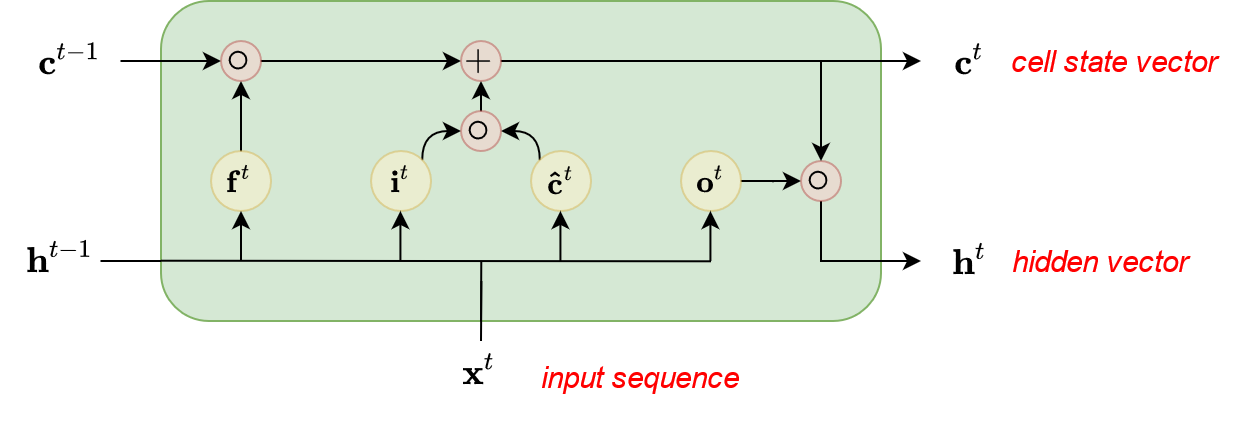
\includegraphics[width=1.\linewidth]{Images/chap3/lstm.png}
    \captionof{figure}[Long short-term memory cell mechanism]{Long short-term memory cell mechanism. In this diagram the activation functions are not shown for the sake of clarity. The gates are displayed in yellow whereas the operations are in red, with $\circ$ denoting the Hadamard (element-wise) product.}
    \label{fig:lstm}
    \end{center}
\end{figure}

The long short-term memory (LSTM) is a recurrent architecture proposed in 1997 by Hochreiter and Schmidhuber \cite{hochreiter_long_1997}, as a means to cope with the vanishing gradient problem, by keeping the error in the LSTM cells. Fig.~\ref{fig:lstm} illustrates the mechanism behind an LSTM cell. In addition to the input vector $\mathbf{x}^t$ and the hidden vector $\mathbf{h}^t$, this model introduces new vectors which are used as \textit{gates} to control the flow of information inside the LSTM cell. The first four vectors, which are all computed in a similar way with their own weights, are:
\begin{itemize}
    \item a forget gate vector $\mathbf{f}^t$ obtained by:
    \begin{equation}
        \mathbf{f}^t = \sigma_s(\mathbf{W}_{f,x} \mathbf{x}^t + \mathbf{W}_{f,h} \mathbf{h}^{t-1} + \mathbf{b}_f),
    \end{equation}
    
    \item an input gate vector $\mathbf{i}^t$ computed with:
    \begin{equation}
        \mathbf{i}^t = \sigma_s(\mathbf{W}_{i,x} \mathbf{x}^t + \mathbf{W}_{i,h} \mathbf{h}^{t-1} + \mathbf{b}_i),
    \end{equation}
    
    \item an output gate vector $\mathbf{o}^t$ expressed by:
    \begin{equation}
        \mathbf{o}^t = \sigma_s(\mathbf{W}_{o,x} \mathbf{x}^t + \mathbf{W}_{o,h} \mathbf{h}^{t-1} + \mathbf{b}_o),
    \end{equation}
    
    \item a cell input activation vector $\mathbf{\hat{c}}^t$ calculated from
    \begin{equation}
        \mathbf{\hat{c}}^t = \sigma_h(\mathbf{W}_{c,x} \mathbf{x}^t + \mathbf{W}_{c,h} \mathbf{h}^{t-1} + \mathbf{b}_c),
    \end{equation}
\end{itemize}
where $\sigma_s$ and $\sigma_h$ are the sigmoid and hyperbolic tangent activation functions, respectively. 

Using the $\mathbf{x}^t$, $\mathbf{i}^t$, $\mathbf{f}^t$ and $\mathbf{\hat{c}}^t$, the cell state vector $\mathbf{c}^t$ (acting like a memory cell), can be obtained by:
\begin{equation}
    \mathbf{c}^t = \mathbf{f} \circ \mathbf{c}^{t-1} + \mathbf{i}^t \circ \mathbf{\hat{c}}^t,
\end{equation}
where $\circ$ denotes the element-wise product.
Finally, the hidden vector $\mathbf{h}_t$ is computed with:
\begin{equation}
    \mathbf{h}_t = \mathbf{o}^t \circ \sigma_h(\mathbf{c}^t).
\end{equation}
In an LSTM cell, the hidden vector $\mathbf{h}^t$ actually acts as the output vector at each timestep $t$.\footnote{Although this seems to contrast with the definition of an RNN, it is actually the way the LSTMs are implemented in most deep learning frameworks such as \textit{Tensorflow} or \textit{PyTorch}.}

\subsection{Gated recurrent units}

\begin{figure}[t]
    \begin{center}
    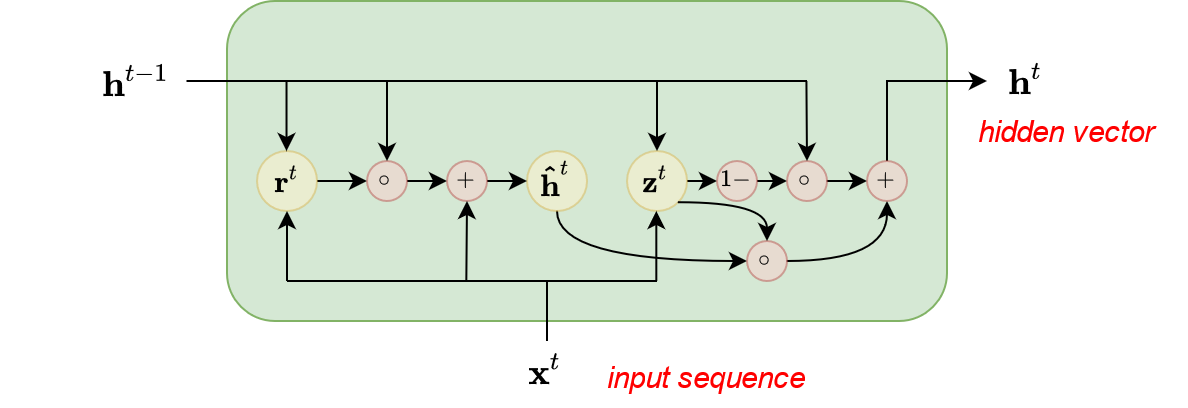
\includegraphics[width=0.9\linewidth]{Images/chap3/gru.png}
    \captionof{figure}[Gated recurrent unit mechanism]{Gated recurrent unit mechanism.}
    \label{fig:gru}
    \end{center}
\end{figure}

In the same vein as LSTMs, gated recurrent units (GRU) \cite{cho_learning_2014} have an internal mechanism which can circumvent the vanishing gradient problem as the error remains in the GRU cells. A GRU is composed of two gate vectors, as illustrated in Fig.~\ref{fig:gru}:
\begin{itemize}
    \item an update gate vector $\mathbf{z}^t$ obtained by:
    \begin{equation}
        \mathbf{z}^t = \sigma_s(\mathbf{W}_{z,x} \mathbf{x}^t + \mathbf{W}_{z,h} \mathbf{h}^{t-1} + \mathbf{b}_z),
    \end{equation}
    
    \item a reset gate vector $\mathbf{r}^t$ computed with:
    \begin{equation}
        \mathbf{r}^t = \sigma_s(\mathbf{W}_{r,x} \mathbf{x}^t + \mathbf{W}_{r,h} \mathbf{h}^{t-1} + \mathbf{b}_r).
    \end{equation}
\end{itemize}
A candidate activation vector is then calculated with:
\begin{equation}
    \mathbf{\hat{h}}^t = \sigma_h\big(\mathbf{W}_{h,x} \mathbf{x}^t + \mathbf{W}_{r,h} (\mathbf{r}^t \circ \mathbf{h}^{t-1} + \mathbf{b}_h)\big).
\end{equation}
Finally the hidden vector (also acting as the output vector) is obtained with:
\begin{equation}
    \mathbf{h}^t = (1-\mathbf{z}^t) \circ \mathbf{h}^{t-1} + \mathbf{z}^t \circ \mathbf{\hat{h}}^t.
\end{equation}
In summary, a GRU is similar to an LSTM, with the main difference that a single gate performs both the forgetting and updating actions.

\subsection{Bidirectional recurrent layers}

\begin{figure}[t]
    \begin{center}
    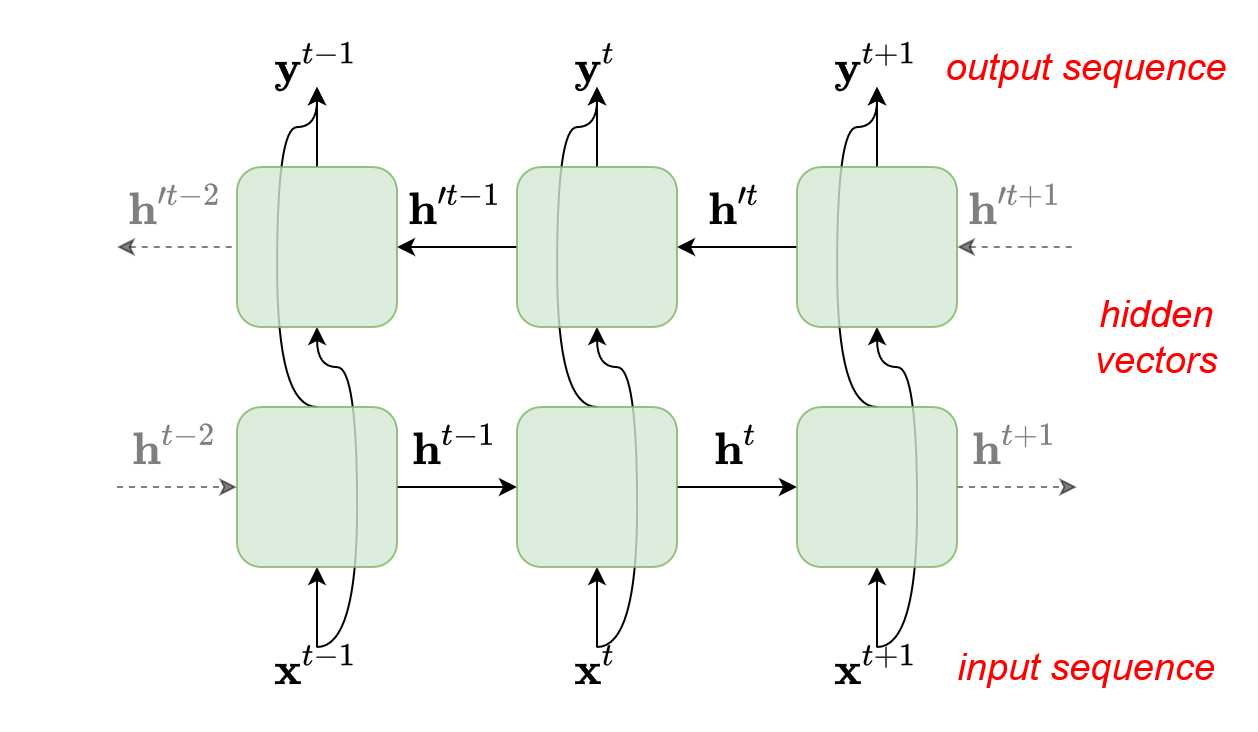
\includegraphics[width=1.\linewidth]{Images/chap3/bidirectionalRecurrentNeuralNetworks.png}
    \captionof{figure}[Bidirectional recurrent neural networks]{Bidirectional recurrent neural networks. A sequence is processed in both directions: from past to future and from future to past. This scheme can be applied for any recurrent mechanism, \textit{i.e.}, the green cells can be basic recurrent units, LSTMs or GRUs.}
    \label{fig:bidirectionalRecurrentNeuralNetworks}
    \end{center}
\end{figure}

The different types of recurrent mechanism presented above (basic recurrent layer, LSTM and GRU) are capable of processing the sequential data in a causal way. However, depending on the learning task, it could be meaningful to process the data in the other direction as well, from future to current input  (\emph{e.g.}, when looking for a music tempo, or when a whole data sequence is analyzed to obtain an overall prediction). In other words, it can be interesting to exploit information from both past and future data when processing the data at the current timestep. Bidirectional recurrent neural networks \cite{schuster_bidirectional_1997} have been introduced to address this problem. They combine recurrent layers processing the sequence from beginning to the end with recurrent layers processing the sequence the other way around. Fig~\ref{fig:bidirectionalRecurrentNeuralNetworks} illustrates how such a combination is done within the network. An input vector is fed separately into a forward layer and a backward layer, each one producing an independent output internal state vector. Thus, the next layer can benefit from two input vectors, one relying on the past and another relying on the future. Such bidirectional layers can also be applied with LSTMs or GRUs.

%-----------------------------------------------
%  RESIDUAL CONNECTIONS
%-----------------------------------------------
\section{Residual neural networks}
\label{ss:residualNetworks}

In this section we briefly present what residual neural networks consist of, and why are they useful in deep learning models.

Residual neural networks have been proposed in 2016 by He et al.~\cite{he_deep_2016} to address two common training problems encountered with very deep convolutional neural networks: the vanishing gradient problem which we presented in Section~\ref{ss:recurrentNeuralNetworks}, and the loss of accuracy resulting from the large number of layers. Their idea actually improved the performance of convolutional neural networks because it allowed for deeper architectures.

Residual neural networks are based on the desire of preserving the input features of a given layer, in addition to the output of this layer. Indeed, numerous successive transformations, applied by the multilayer structure of a deep neural network, can result in the loss of meaningful information contained in the layer's input features. By adding \textit{residual connections} between the input of a layer and its output, one can make this input feature flow through this layer unaltered (or almost, as we will see) so that it can be used further in the network.

\begin{figure}[t]
    \begin{center}
    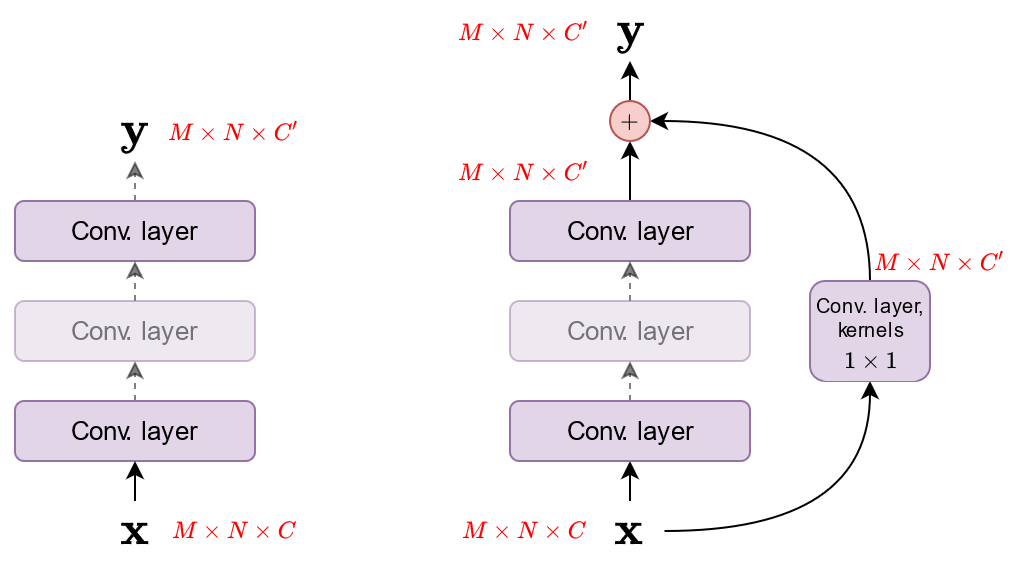
\includegraphics[width=1.\linewidth]{Images/chap3/residualBlock.png}
    \captionof{figure}[Comparison of a residual block and a classical convolutional block]{Comparison of a residual block (right) and a classical convolutional block (left). In a residual block, the input is added to the output of the last convolutional layer, eventually after its shape is adjusted using an additional convolutional layer to match the shapes.}
    \label{fig:residualBlock}
    \end{center}
\end{figure}

Fig.~\ref{fig:residualBlock} illustrates how a residual block, \emph{i.e.}, a series of layers including a residual connection, differs from a similar neural network segment without such connections. As we can see, the input of this block flows through the residual connection and is added to the output of the residual block. This residual block transforms the input using several layers, as a classical convolutional neural network usually does. However, in order to be able to add the input with the residual block output, we need to make sure to match their shapes. One trick to do this relies on inserting a convolutional layer with kernels of size $1 \times 1$ to adapt the dimensions of the input feature.

An extension of this idea has been proposed in \cite{huang_densely_2017}, where the authors propose to concatenate the input of one block with its output, instead of adding them. Their goal is to have every feature map propagated in each subsequent layer.

%-----------------------------------------------
%  ATTENTION MECHANISM
%-----------------------------------------------
\section{Attention mechanisms}
\label{sec:attentionMechanisms}


In this section we explain the attention and self-attention mechanisms. Attention models were introduced by Badhanau et al. \cite{bahdanau_neural_2015} in 2014 and refined by Luong et al. \cite{luong_effective_2015} in 2015 to improve sequence-to-sequence models. It granted neural networks with the capability to cope with long input sequences, especially in machine translation. Another great leap in natural language processing (NLP) was made with the Transformer architecture \cite{vaswani_attention_2017}, which includes the concept of \textit{self-attention}. This neural network based on an encoder-decoder scheme is very powerful to exploit the context of each word in a sentence, and has led to state-of-the-art language models such as BERT \cite{devlin_bert_2019} or GPT \cite{brown_language_2020}.

\subsection{Encoder-decoder scheme}

A sequence-to-sequence model is an architecture that takes a sequence of items (words, frames, images, etc.) as input, and process it to output another sequence of items. Such models are often constituted of two components: an encoder and a decoder. As illustrated in Fig.~\ref{fig:encoderDecoder}, an encoder is a neural network which processes the entire input sequence and computes an output vector called the \textit{context} vector. This context vector is then sent to the decoder, which is also a neural network, to output the final sequence. Before the advent of attention models, encoder and decoder were usually made of recurrent neural networks, where the context vector is actually the hidden vector of the last recurrent layer of the encoder network. The output sequence is generated item by item by the decoder, at each timestep, using the context vector to initialize its first hidden vector.

\begin{figure}[t]
    \begin{center}
    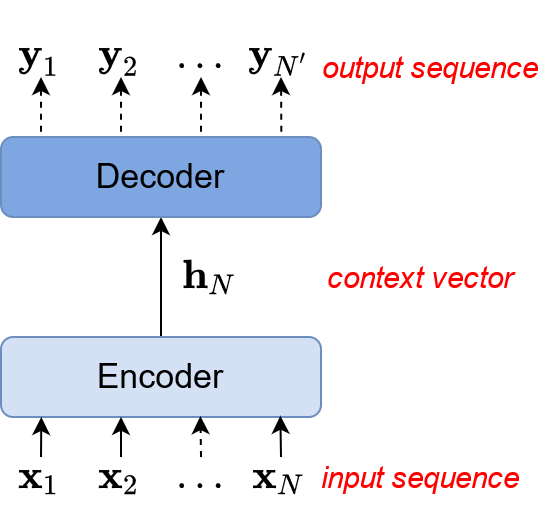
\includegraphics[width=0.5\linewidth]{Images/chap3/encoderDecoder.png}
    \captionof{figure}[Encoder-decoder scheme]{Encoder-decoder scheme. The encoder processes the entire input sequence and produces a context vector, which is then used as input for the decoder part to generate the output sequence. The input and output sequences are not necessarily of the same length.}
    \label{fig:encoderDecoder}
    \end{center}
\end{figure}


\subsection{Concept of attention}
\label{sec:attention}

As we have seen, the context vector contains all information available to the decoder to generate the output sequence. This is an issue when dealing with long input sequences, since it becomes more and more difficult to encode all relevant information from such a sequence in a single vector. Attention has been conceived to circumvent this limitation.

The first addition to the previously explained encoder-decoder scheme is that the encoder hidden vectors for all steps are passed to the decoder, instead of passing only the last hidden vector. In that way, information from each input sequence item is available to the decoder. The second novelty is the so-called attention step. The intuition is that, with regards to a particular output item, there are some items in the input sequence which are more relevant than the others. Assuming the decoder is at timestep $t$, meaning it has already output $t-1$ items, and the current hidden vector is $\mathbf{h}_{t-1}$, the attention mechanism works as follows:
\begin{itemize}
    \item a so-called \emph{attention score} is computed between all encoder hidden vectors and the current decoder hidden vector $\mathbf{h}_{t-1}$, by the means of learnable weights matrices;
    \item a softmax function is applied to all obtained attention scores so that their sum is $1$;
    \item a weighted sum of all encoder hidden vectors is calculated, using their respective softmaxed attention scores, leading to the ``current'' \textit{context} vector relevant to $\mathbf{h}_{t-1}$.
\end{itemize}
This context vector thus contains all the information about the input sequence items that is useful for the processing of the current timestep. In \cite{bahdanau_neural_2015}, the attention scores are obtained with a feedforward neural network, trained altogether with the other neural network parts. After this attention stage, the context vector is concatenated with $\mathbf{h}_{t-1}$ and is fed into another feedforward neural network, whose output is taken as the next output sequence item.

As we can see, the idea behind the attention mechanism is to provide a way for the decoding neural network to emphasize some of the input sequence items, regarding the current decoding timestep.

\subsection{Self-attention in the Transformer architecture}

The Transformer architecture is a model solely relying on the attention mechanisms, whereas previously presented models were designed as a mix of RNNs and attention. It has been proposed in 2017 by Vaswani et al. \cite{vaswani_attention_2017}, outperforming the previous models, while being more parallelizable and requiring less training time. The Transformer model is also made of encoding and decoding modules, but here each one includes several (internal) encoders and decoders, respectively. All such encoders are identical and process the input sequence items one after another.

Fig.~\ref{fig:transformerEncoder} shows the components included in one encoder. It is composed of a self-attention module, which is an attention block that compares the input sequence with itself, \emph{i.e.}, it compares each item $\mathbf{x}_i$ with the other items in the same sequence, and outputs a new corresponding vector $\mathbf{z}_i$. Then each vector $\mathbf{z}_i$ is passed independently through the same feedforward layer. The output of the encoder is therefore a new sequence of the same size as the input sequence, which can then used as the input sequence of the next encoder. 

\begin{figure}[t]
    \begin{center}
    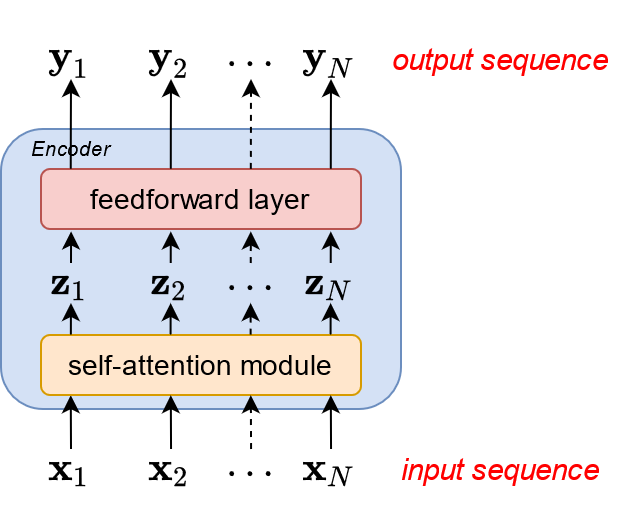
\includegraphics[width=0.6\linewidth]{Images/chap3/transformerEncoder.png}
    \captionof{figure}[Transformer's encoder components]{Transformer's encoder components. A self-attention module creates an intermediate vector $\mathbf{z}_i$ for each vector $\mathbf{x}_i$ of the input sequence. Each vector $\mathbf{z}_i$ then passed independently in a feedforward layer which produces an output sequence of the same size as the input sequence. The output sequence usually becomes the input sequence of another encoder as several encoders are stacked one after another in a typical Transformer architecture.}
    \label{fig:transformerEncoder}
    \end{center}
\end{figure}


\begin{figure}[t]
    \begin{center}
    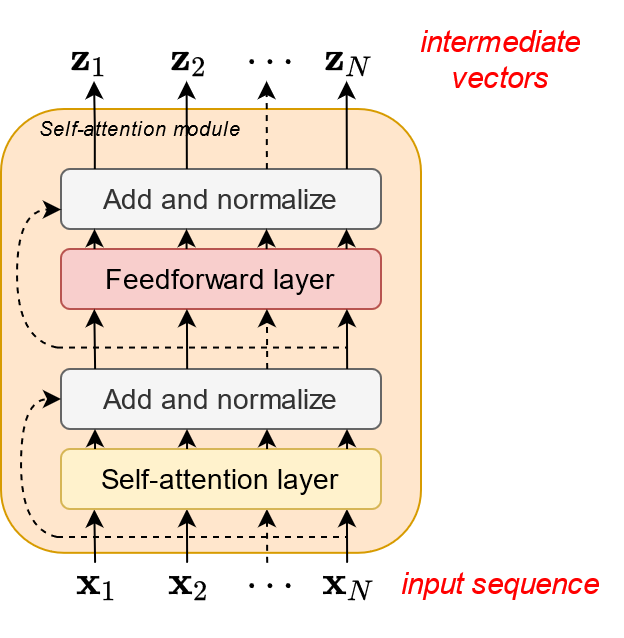
\includegraphics[width=0.6\linewidth]{Images/chap3/selfAttentionModule.png}
    \captionof{figure}[Self-attention module]{Self-attention module. In a self-attention module, the input sequence is first processed by a self-attention layer, of which the output is added to the input (using a residual connection) and the result is normalized. Then, each item of the obtained sequence goes independently through the same feedfoward layer, and the new sequence is again added to the forward layer's input sequence using a residual connection, then is normalized. Note that positional encoding, which is usually used in such encoder architecture, is not shown here as it was not used in this thesis work.}
    \label{fig:selfAttentionModule}
    \end{center}
\end{figure}

The self-attention module is illustrated in Fig.~\ref{fig:selfAttentionModule}. First, a self-attention layer actually performs the self-attention mechanism on the input sequence. For each item of the sequence $\mathbf{x}_i$, three vectors usually named \textit{query}, \textit{key}, and \textit{value} are computed. They are obtained by multiplying $\mathbf{x}_i$ with three independent weight matrices that are learnt during the training:
\begin{equation}
    \begin{aligned} 
      \mathbf{q}_i &= \mathbf{x}_i^T \mathbf{W}^Q \\
      \mathbf{k}_i &= \mathbf{x}_i^T \mathbf{W}^K. \\
      \mathbf{v}_i &= \mathbf{x}_i^T \mathbf{W}^V
    \end{aligned}
\end{equation}
Then, when encoding the item $\mathbf{x}_i$, a score $s_{ij}$ is computed with respect to every other item $\mathbf{x}_j$ as \cite{vaswani_attention_2017}:
\begin{equation}
    s_{ij} = softmax \bigg( \frac{\mathbf{q}_i \cdot \mathbf{k}_j}{\sqrt{G}} \bigg),
\end{equation}
where $G$ is the dimension of the key vectors. Finally, a new vector $\mathbf{z}_i$ is calculated as the weighted sum of the value vectors $\mathbf{v}_j$, using the computed scores as weights:
\begin{equation}
    \mathbf{z}_i = \sum_{j=1}^N s_{ij} \mathbf{v}_j,
\end{equation}
with $N$ being the sequence length. For each input sequence item $\mathbf{x}_i$ we thus obtain a new vector $\mathbf{z}_i$ that takes into account the dependencies between $\mathbf{x}_i$ and the other items (past and future) in the sequence.

The remaining components of the self-attention module shown in Fig.~\ref{fig:selfAttentionModule} are the following: a layer adds the input of the encoder to the output of the self-attention layer (sequence-wise) using a residual connection, and then normalization is applied; then each item of the obtained sequence goes independently through the same feedfoward layer, is added with the corresponding input item of this layer, with another residual connection, and is also normalized.

A last particularity for the encoder is proposed in the original paper \cite{vaswani_attention_2017}, and is called \textit{positional encoding}. The authors propose to encode the position of each input vector within the sequence using a vector $\mathbf{p}_i$ (we do not detail such encoding here, \emph{c.f.}, \cite{vaswani_attention_2017}), and append this position vector to the corresponding item $\mathbf{x}_i$, before going through the encoder.

\begin{figure}[t]
    \begin{center}
    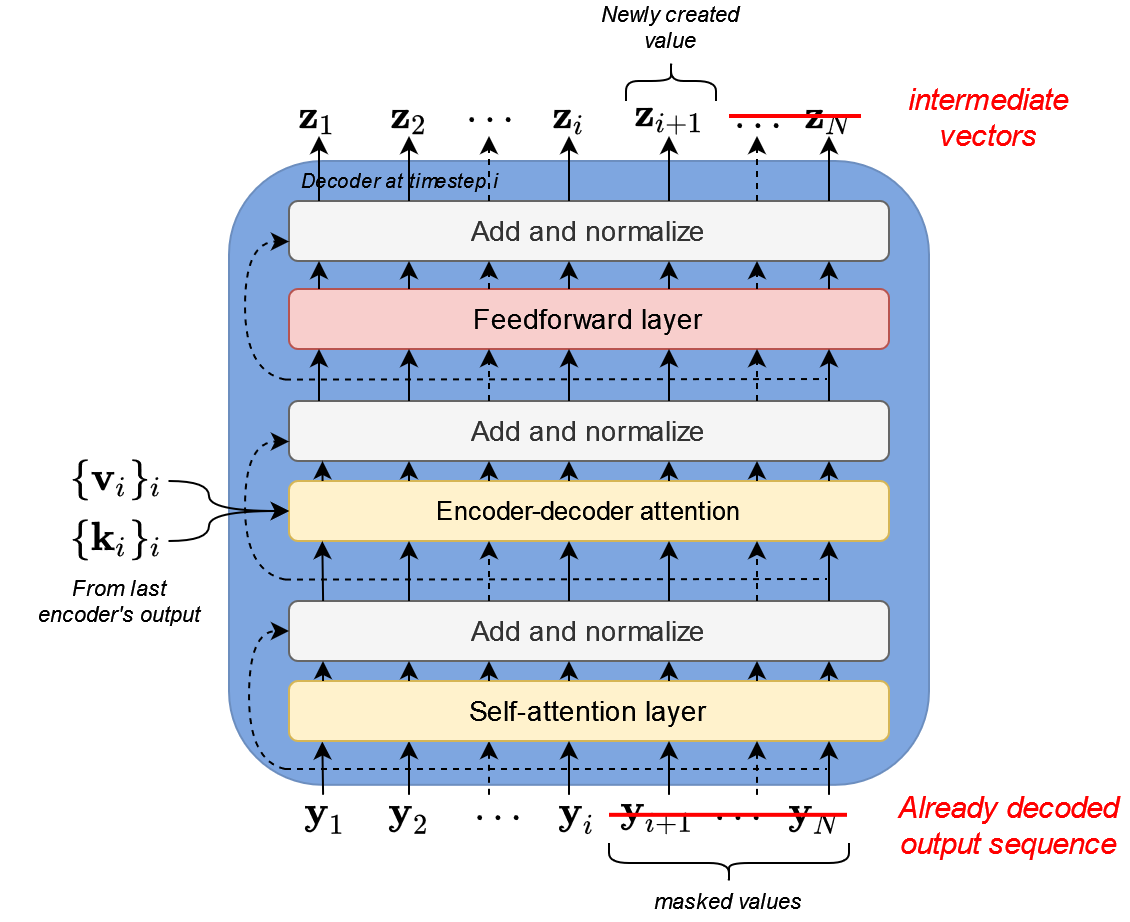
\includegraphics[width=0.85\linewidth]{Images/chap3/transformerDecoder.png}
    \captionof{figure}[Transformer's decoder module at timestep $i$]{Transformer's decoder module at timestep $i$. After a self-attention module followed by an add and normalize layer, a encoder-decoder attention module is used, and followed by another add and normalize layer. This encoder-decoder attention actually uses the key and value vectors obtained from the last encoder. Then a feedforward layer followed by an add and normalize layer is used as in en encoder module. As for the encoders, several decoders are employed and stacked one after another. As timestep $i$ (\emph{i.e.}, when decoding item $i$ of the output sequence), the previous items $1, ..., i-1$ are already decoded, and are used in the input sequence of the first decoder. The other items $i+1, ..., N$, not yet decoded, are masked in the input sequence. The newly created output item $i+1$ of the last decoder is finally used through a final layer which projects it into the target embedding space.}
    \label{fig:transformerDecoder}
    \end{center}
\end{figure}

Let us now briefly detail how the Transformer decoder part works, without going too much into details since in this thesis we only adopted the encoder in our experiments. A decoder module, illustrated in Fig.~\ref{fig:transformerDecoder}, is made of a self-attention layer, which receives the already encoded output items (the future items, not created yet, are masked during the process), followed by an add and normalize layer with residual connection. The obtained sequence is fed into another similar attention block called \textit{encoder-decoder attention} because its key and value vectors are those obtained from the output sequence of the last encoder. Finally, as in a encoder module, each obtained sequence item goes through the same feedforward layer, and then another add and normalize layer with residual connection is used. At the end, each item of the output sequence of the last decoder is projected into the target embedding space using a linear feedforward neural network, leading to the final output sequence.

\subsection{Multi-head self-attention}

In \cite{vaswani_attention_2017}, the authors actually used an extended version of the self-attention mechanism presented above. In \textit{multi-head} self-attention (MHSA), several instances of the query, key and value vectors are computed in parallel, with corresponding weights matrices $\mathbf{W}^Q$, $\mathbf{W}^K$ and $\mathbf{W}^V$. This allows a self-attention module to learn several representations for the three vectors of each item in the sequence, leading to more flexibility. When considering $H$ heads, for each item $\mathbf{x}_i$ in the input sequence we obtain $H$ vectors $\mathbf{z}_{ih}$ ($h \in [1,H]$) which are concatenated along the head dimension to give $\mathbf{\tilde{z}}_i$, and a new weight matrix $\mathbf{W}^O$ is used to obtain the final output vector $\mathbf{z}_i$:
\begin{equation}
    \mathbf{z}_i = \mathbf{\tilde{z}}_{i} \mathbf{W}^O. 
\end{equation}

In the original paper \cite{vaswani_attention_2017}, the operations to compute the self-attention scores consider the query and key vectors independently per head, \emph{i.e.}, the score for pair of item $(i,j)$ and for head $h$ is obtained by :
\begin{equation}
    s_{ijh} = \text{softmax}\Big(\frac{\mathbf{q}_{ih} \cdot \mathbf{k}_{jh}}{\sqrt{G}}\Big),
\end{equation}
where $q_{ih}$ is the query vector of item $\mathbf{x}_i$ for head $h$, and $k_{jh}$ is the key vector of item $\mathbf{x}_j$ for the same head $h$. A more general way of calculating the scores is to consider the query and key vectors across different heads $h$ and $h'$:
\begin{equation}
\label{eq:crossMultiHeadScores}
    s_{ijhh'} = \text{softmax}\Big(\frac{\mathbf{q}_{ih} \cdot \mathbf{k}_{jh'}}{\sqrt{G}}\Big).
\end{equation}
We call this more general computation \textit{cross multi-head} self-attention (CMHSA), however we did not find any literature reference considering such a mechanism. \footnote{As we will explain in a series of experiments in Sec.~\ref{chap:multisourceLocalization}, we actually performed cross-multi-head self-attention by accident while tuning our models. After investigations we understood that the scores were computed as in \eqref{eq:crossMultiHeadScores} whereas we never encountered this in the literature. We nevertheless kept these ideas since it gave interesting results} Mathematically, we can interpret a cross-multi-head mechanism with $H$ as a classical multi-head self-attention with $H^2$ heads where the query and key matrices share weights.

%-----------------------------------------------
%  CONCLUSION
%-----------------------------------------------
\section{Conclusion}
In this chapter, we provided a quick overview on different deep learning architectures that were used for designing neural models in this thesis. After presenting the basics of neuron mechanisms, we showed how feedforward neural networks, recurrent neural networks and convolutional neural networks can perform some particular tasks. We also briefly explained how residual connections work and why they are of interest. Finally, we described the basics of attention mechanism and Transformer architecture with self-attention, which are quite recent neural methods in the audio literature. Convolutional recurrent neural networks and attention mechanisms have been particularly considered in our experiments on sound source localization.

\chapter{State-of-the-art on speaker counting and localization}
\label{chap:soa}

\lettrine{I}{n} this chapter, we provide a literature survey addressing speaker counting and localization. We limit the scope of the survey to methods evaluated on speech signals as it was the focus of this thesis. In the Section~\ref{sec:countingLiterature}, we describe the relatively scarce literature on speaker counting, including parametric, clustering and deep learning methods. In Section~\ref{sec:SSLliterature}, we address the literature on sound source localization, by first quickly presenting conventional\footnote{We define as ``conventional'' the methods based on traditional signal processing techniques, without deep learning.} methods, and then providing a short survey of SSL systems using deep learning techniques. As a more exhaustive survey of these neural-based SSL methods has been submitted at the time of this thesis writing \cite{grumiaux_survey_2021}, in this section we limit our description on methods in relation with our research. 

%-----------------------------------------------
%  SPEAKER COUNTING
%-----------------------------------------------
\section{Speaker counting}
\label{sec:countingLiterature}

Speaker counting is the task of estimating the number of people that are speaking in an audio signal. It can be seen as a subtask of speaker diarization, whose objective is to detect which speaker is active at what moment. Most approaches actually focus on predicting the total number of speakers in the analyzed signals, but we found some works considering the instantaneous NoS or the maximum number of simultaneous speakers (see Section~\ref{ss:sourceCounting} for a mathematical definition). Note that in a lot of system, the total and maximum NoS are actually identical since they supposed a constant NoS through the whoel analyzed signal. 

Speaker counting has not often been addressed in the speech processing literature as a separate task, although it is a useful information for other more complex speech-related tasks such as speaker diarization or speech signals separation. Many such systems actually assume the knowledge of the number of speakers, even though we do not have it at hand in practice.

\subsection{Parametric methods}

Early methods for speaker counting attempted to correlate the number of speakers to some features extracted from the audio signal. In \cite{arai_estimating_2003}, the authors proposed to exploit the modulation characteristics of the human voice to correlate the modulation index calculated from the input signal, and the total number of speakers. They computed a function of the modulation index which outputs the number of speakers based on several multi-speaker signals constructed from TIMIT excerpts \cite{garofolo_timit_1993}, containing up to 8 simultaneous speakers. Another parameter, derived from the statistics of a particular mel filter coefficient, has been proposed in \cite{sayoud_proposal_2010} to estimate the total number of speakers in a single-channel mixture. The authors related these statistics directly with the number of speakers via a polynomial function. In \cite{pasha_towards_2017}, a parametric method has been derived for speaker counting, which relies on coherent-to-diffuse ratio estimation over several time frames. The maximum number of speakers $\bar{J}$ is then estimated by thresholding this computed parameter.

\subsection{Clustering methods}

A few counting methods based on clustering algorithms have been proposed in the literature to address source counting along with other tasks, such as source localization or separation. In \cite{arberet_robust_2010}, an algorithm named DEMIX is derived to jointly count, locate and separate up to 6 sources in a multi-channel recording. This method has been applied for speech signals and works in an underdetermined setting, but is however limited to an anechoic environment. Another clustering scheme can be found in \cite{yang_multiple_2017} in which the principal eigenvectors of the covariance matrix of a multi-channel signal are extracted to estimate the total number of sources. It showed to be quite robust for speech recordings with signal-to-noise ratios (SNR) between $0$ and $20$~dB, in environments with low reverberation (TR60 = $250$~ms). In \cite{xu_crowd++:_2013}, the authors use a clustering algorithm to aggregate the mel-frequency cepstrum coefficients (MFCC) computed from successive speech segments extracted from a single-channel audio mixture. Using a cosine similarity, the clustering algorithm compares pairs of MFCC features to aggregate them into a certain number of classes, which corresponds to the estimated total number of speakers.


\subsection{Deep learning methods}

Several recent works have used neural networks to estimate the number of speakers. To the best of our knowledge, the first deep-learning-based method for speaking counting has been proposed in \cite{stoter_classification_2018}. The authors aim to estimate the maximum number of concurrent speakers $\bar{J}$ in a $5$-s single-channel audio mixture, containing at most $10$ speakers. The classification paradigm and the regression paradigm (see Section~\ref{ss:outputScheme} for more details) are compared, using a neural network consisting of bidirectional LSTM layers. The article further evaluates the use of different input features. The presented results indicate the superiority of classification over regression for speaker counting, and that STFT features yield the best performance. The authors extended this work in \cite{stoter_countnet:_2019} by evaluating more neural network architectures, including CNN, RNN and CRNN. They compare the use of usual $3 \times 3$ convolutional kernels with full-band convolutional filters of size $1 \times F$, with $F$ the number of frequency bins. The results indicate that a CRNN with $3 \times 3$ filters leads to the best performance. Their study also includes the use of different datasets, the evaluation of several reverberation time values, and a comparison of their system against human capabilities. 

In the same vein, a speaker counting CNN is proposed in \cite{wei_determining_2018}, capable of categorizing the input signal as containing $1$, $2$ or $3$ and more speakers. In \cite{andrei_overlapped_2019}, an interesting comparison on the human abilities for speaker counting and their machine counterpart is proposed. The authors show that machine algorithms can surpass human level performance, especially when the analysis time is short. Temporal convolutional networks (TCN) have been applied in \cite{cornell_detecting_2020} to count the maximum number of overlapping speakers in a single-channel mixture, as in \cite{stoter_classification_2018}. They show that TCN improves the counting accuracy compared to CRNNs and LSTM-based networks on real data. In \cite{wang_speaker_2020}, a neural-based speaker counting system is trained using transfer learning based on SincNet \cite{ravanelli_speaker_2018}, a speaker recognition network. The output of a truncated version of the already trained SincNet is used as an input feature of their speaker counting system, along with the zero-crossing rate, the spectral spread and the spectral entropy of the input signal. All these features are fed in a feedforward neural network to estimate up to $10$ speakers. Peng \textit{et al.}~\cite{peng_competing_2020} proposed to train a recurrent neural network to project the input features, composed of log-spectra and interaural phase differences (IPDs), extracted from multi-channel signals, into an embedding space. The number of speakers can be obtained as the rank of the covariance matrix of the embedded vectors. An attention-based network is explored in \cite{yousefi_real-time_2021} for speaker counting. After a series of convolutional layers for feature extraction, an attention mechanism is trained to aggregate temporal information in a new feature vector. This vector is then fed into a feedforward layer for the final estimation of the number of speakers.

As estimating the number of speakers is generally done to provide another speech-related task with a precious piece of information, a few works has been proposed to jointly tackle the considered speech processing task and the speaker counting problem. Several speaker diarization/separation systems are trained to simultaneously count and separate speech signals \cite{von_neumann_all-neural_2019,kinoshita_tackling_2020}. These systems do not explicitly estimate the number of speakers, but rather extract the speech signals in a recursive manner. Another joint speaker counting and separation system is proposed in \cite{xiao_improved_2020}, relying on an encoder-decoder architecture. The vector obtained at the bottleneck of the encoder-decoder network is projected into a embedding space, giving a set of embedded vectors whose covariance matrix rank gives the number of sources in the mixture, as in \cite{peng_competing_2020}. In \cite{nguyen_robust_2020}, the authors jointly estimate the number of sources and their respective direction-of-arrivals (DoAs, see Section~\ref{sec:SSLliterature}) by designing a CNN which separates into two distinct branches after a series of convolutional layers: one branch is trained to output the number of sources and another estimate the DoAs. They evaluate their system on speech signals and sound events showing better counting accuracy than DoA-based methods. 


\subsection{Thesis position}

All the above-mentioned and recently proposed DL-based counting methods have shown promising results over conventional methods. Our research for estimating the number of speakers followed this trend. When the present PhD research work was carried out, in the beginning of 2019, the use of neural networks for speech source counting was a pioneering idea and all the related works were limited to single-channel signals. This motivated our effort to improve speaker counting with multi-channel signals in the hope of taking benefit of spatial information in addition to spectral content. Moreover, most systems considered the estimation of the total number of sources $J$, sometimes over audio segments of several seconds, although the instantaneous NoS $J(t)$ often varies along the signal. In our research, we rather focused on this instantaneous NoS $J(t)$. Another aspect that we address was the temporal resolution of the counting system, as most of the speech/audio source counting literature, at the time of our experiments, considered a quite large temporal context, which could be insufficient for online systems or for applications that require a good temporal resolution, such as speech signals separation. Finally, we made use of Ambisonics features, as for all the remaining of this thesis, which had never been proposed in the counting literature. The interest of such signal representation has been discussed in Chapter~\ref{chap:ambisonics} and we assumed that it would be also appropriate for the speaker counting task since spatial information can help to detect spatially distinct speakers.

%-----------------------------------------------
%  SOUND SOURCE LOCALIZATION
%-----------------------------------------------
\section{Sound source localization}
\label{sec:SSLliterature}

The sound source localization problem has been thoroughly studied for decades, often with a focus on speech signals. A large variety of methods have been designed to address SSL in different scenarios, in anechoic and reverberant conditions, considering one or more sources, static or moving in the environment. In this section, after first presenting a short description of conventional SSL methods based on signal processing, we focus on deep-learning-based SSL techniques, as these have recently become a hot topic in the literature. We put an emphasis on neural SSL systems related to this thesis research.

\subsection{Traditional signal processing methods}

\subsubsection{Time difference of arrival}

When multiple microphones are used to record a sound field, the signal incoming from a point source arrives at different instants at each microphone. The time difference of arrival (TDoA), between pairs of microphones, contains information about the direction of the source if the arrangement of the microphones is known. The TDoA can be estimated as the time lag corresponding to the maximum of the cross-correlation function between a pair of microphones. However, in real conditions it is blurred by noise and reverberation. To improve the robustness of this technique, Knapp and Carter \cite{knapp_generalized_1976} introduced in 1976 \textit{generalized cross-correlation with phase transform} (GCC-PHAT), which is computed by dividing the cross-correlation by its amplitude. This can be computed using the signals of a microphone pair $(i,i')$, for a time frame $t$ and a lag $\tau$, by summing over all frequencies $f$:
\begin{equation}
\label{eq:gcc_phat}
    \Psi_{ii'}(t,\tau) = \frac{1}{F} \sum_{f=0}^{F-1} \frac{x_i(t,f) x^{*}_{i'}(t,f)}{\mid x_i(t,f) \mid \mid x_{i'}(t,f) \mid} e^{2 i \pi \tau \frac{f}{F}},
\end{equation}
where $F$ is the total number of  frequencies, and $x_i(t,f)$ and $x_{i'}(t,f)$ are the signals in the STFT domain from microphones $i$ and $i'$, respectively.
Then the corresponding TDoA $\Delta_{ii'}(t)$ can be deduced as:
\begin{equation}
    \Delta_{ii'}(t) = \argmax_{\tau} \Psi_{ii'}(t,\tau).
\end{equation}
Because of the demoninator in \eqref{eq:gcc_phat}, the GCC-PHAT method is quite sensitive to noise, and besides is poorly robust in the presence of multiple sources \cite{blandin_multi-source_2012}.

Many neural-based SSL methods rely on GCC-PHAT features as input for a localization neural network \cite{xiao_learning-based_2015, vesperini_neural_2016, li_online_2018, comanducci_source_2020, vera-diaz_towards_2021} (see Section~\ref{ss:neuralSSL} for a more detailed survey of SSL with neural networks).

\subsubsection{Acoustic maps}

Another way to localize sound sources is to generate \textit{acoustic maps}, which relate the energy or power of acoustic signals to predefined search directions (\emph{e.g.}, on a discrete grid). The steered response power (SRP) can be used to generate such maps, and similarly to GCC-PHAT, it has also been adapted with the phase transform, resulting into the SRP-PHAT algorithm \cite{dmochowski_generalized_2007}. Such an acoustic map can be obtained by scanning the whole space with a beamformer and computing the signal energy or power for each considered direction.

Because of the amplitude normalization and the averaging across all microphone pairs, this method is more robust to reverberation, however it has the undesired effect of emphasizing time-frequency bins containing only noise.

Neural networks have been used to improve the robustness of the SRP-PHAT algorithm. In \cite{pertila_robust_2017}, a CNN has been trained to estimate a time-frequency (TF) mask for each microphone signal. These are applied to corresponding STFT representations, prior to computing the GCC-PHAT quantity of each microphone pair. This method shows to be more robust to strong interfering sources and reverberation. Another system, proposed by Diaz-Guerra et al. \cite{diaz-guerra_robust_2021}, relies on a CNN to directly estimate the Cartesian coordinates of a sound source from an SRP-PHAT acoustic map, again improving the performance in reverberant and noisy conditions.

\subsubsection{Subspace methods}

Subspace methods are based on the eigendecomposition of the spatial covariance matrix (SCM) calculated from the observation vectors. In the narrowband \textit{multiple signal classification} (MUSIC) algorithm \cite{schmidt_multiple_1986}, a subset of eigenvectors obtained from the decomposition is attributed to the sources, while the complementary set of eigenvectors is the basis of the noise subspace. The latter are used to compute an acoustic map:
\begin{equation}
    \mathcal{M}(t,f,\theta,\phi) = \frac{1}{\mathbf{a}_{\theta,\phi}^H(f) \mathbf{U}_N(t,f) \mathbf{U}_N^H(t,f) \mathbf{a}_{\theta,\phi}(f)},
\end{equation}
where $\mathbf{U}_N$ is a matrix that contains the noise-related eigenvectors, and $\mathbf{a}_{\theta,\phi}(f)$ is the \textit{steering} vector in direction $(\theta,\phi)$, which represents the delays of the different captures of a plane wave recording at a microphone array. The estimated DoA is obtained with the angles $(\theta,\phi)$ that maximize this acoustic map, thus one needs to probe all considered directions. This time-demanding search can be avoided with another well-known subspace algorithm for source localization, called the estimation of signal parameters via rotational invariance techniques (ESPRIT) \cite{roy_esprit-estimation_1989}, which relies on the source subspace to directly estimate the DoA.

\subsection{Deep learning techniques}
\label{ss:neuralSSL}

In this subsection, we describe different systems that can be found in the DL-based sound source localization literature. We categorize these systems with regards to several aspects: number of sources to localize, network architecture, type of input features, output scheme, learning strategies and training/test datasets. This part of the manuscript is a shortened version of the comprehensive survey of the neural-based literature that we have written and submitted for publication (a preprint version is available \cite{grumiaux_survey_2021}).


\subsubsection{Number of sources}

Many neural-based SSL systems consider only one source to localize, as it is already a very complex problem in real-world environments, due to the presence of noise and reverberation. When the source activity is not controlled artificially, some methods rely on a VAD system as a preprocessing step before localization. It is also possible to simultaneously estimate the source activity \emph{and} perform localization, as in \cite{yalta_sound_2017}. In this work, an additional neuron is appended to the network output, and used to estimate whether the source is active or not. Another way of estimating the NoS alongside localization is to adopt a thresholding method, notably when using a classification paradigm (see Section~\ref{ss:outputScheme}).

Localizing multiple sources is a much harder problem than single-source localization, especially when the activity of the different sources overlaps in time, as we illustrated in Chapter~\ref{chap:introduction}. Nowadays, more and more neural-based localization systems attempt to improve multi-source SSL performance in noisy and reverberant environments. As in the single-source case, many of these multi-source methods assume the NoS $J$ (as described in Section~\ref{ss:sourceCounting}) is known before estimating their locations \cite{hirvonen_classication_2015, chakrabarty_multi-speaker_2017, ma_phased_2018, perotin_crnn-based_2019}, which is then used to estimate the right number of DoAs. In practice, $J$ can be estimated by a dedicated source counting algorithm. An alternative, proposed in a few articles, is to jointly estimate the total number of sources $J$ and their location, either from the localization output \cite{he_joint_2018,moing_learning_2020,sundar_raw_2020}, or by designing a multi-task network trained to also explicitly estimate the NoS \cite{nguyen_robust_2020}. Note that in all these works, the sources are supposed to be static and the NoS is constant, \emph{i.e.}, $J(t) = J, \forall t$.

\subsubsection{Input features}

Many types of input features have been used in the neural SSL literature. Some systems are inspired by signal representations from conventional methods. For instance, GCC-PHAT features have been employed in \cite{xiao_learning-based_2015, vesperini_neural_2016, he_deep_2018, comanducci_source_2020}, while SRP-PHAT-based acoustic maps have been used in \cite{salvati_exploiting_2018, diaz-guerra_robust_2021}. Other features based on cross-correlation functions have been proposed in \cite{grondin_sound_2019, ma_phased_2018}. Ideas from subspace methods have also been exploited in several works. For instance, the eigenvectors of the SCM are fed into neural networks in \cite{takeda_discriminative_2016, takeda_unsupervised_2018}, while in \cite{nguyen_robust_2020} the authors exploit the spatial pseudo-spectrum from the MUSIC algorithm.

Other classical types of features, usually employed in conventional methods, have been reused as input for neural networks. In \cite{chazan_multi-microphone_2019, bianco_semi-supervised_2020}, the authors proposed to compute the relative transfer function (RTF) obtained from all microphone pairs and fed it into the neural network. Other neural SSL systems were designed and used in a binaural set-up, which is a two-microphone format designed to mimic human listening conditions. They thus used classical binaural cues as input features of the network: inter-aural level differences \cite{youssef_learning-based_2013, roden_sound_2015, zermini_deep_2016}, inter-aural time differences \cite{youssef_learning-based_2013, roden_sound_2015}, and  inter-aural phase differences \cite{pak_sound_2019, nguyen_autonomous_2018, sivasankaran_keyword-based_2018, shimada_accdoa_2020, subramanian_deep_2021}.

Low-level representations have also been investigated as neural network inputs, letting the model learn to extract from them the relevant information for localization during the training phase. A number of SSL neural networks proposed in the literature rely on (multi-channel) STFT spectrograms. The network can use only the STFT magnitude \cite{yalta_sound_2017, pertila_robust_2017}, only the STFT phase \cite{subramanian_deep_2021, zhang_robust_2019}, or both \cite{guirguis_seld-tcn_2021, krause_comparison_2021, maruri_gcc-phat_2019, schymura_pilot_2021}. Some systems use the decomposition of complex-valued spectrograms into real and imaginary parts \cite{he_joint_2018, moing_learning_2020}. Finally, a few \textit{end-to-end} neural networks have been designed to estimate the source location directly from the raw multi-channel waveforms. In \cite{suvorov_deep_2018}, the waveforms are fed into 1D convolutional layers, while in other systems \cite{vera-diaz_towards_2018, vecchiotti_end--end_2019, pujol_beamlearning_2021} 2D convolutional layers are preferred.

Finally, many authors chose to take benefit of the Ambisonics format (see Chapter~\ref{chap:ambisonics}) for neural-based SSL. Some of them proposed to feed the network with an Ambisonics spectrogram \cite{adavanne_localization_2019, guirguis_seld-tcn_2021, schymura_exploiting_2021}, while in \cite{comminiello_quaternion_2019} such spectrogram is considered as quaternion-valued and the authors adapted the neural network to operate on such features. The intensity vector is another Ambisonics-based representation that has proven effective for neural-based SSL, according to several articles \cite{perotin_crnn-based_2018, perotin_crnn-based_2019, nguyen_general_2021}. Regarding the Ambisonics order, most of these methods work with the FOA format, but we can find some systems based on the HOA features \cite{varanasi_deep_2020,poschadel_direction_2021}.

\subsubsection{Architectures}

Neural network architectures are probably the most explored aspect of DL-based SSL systems.  The early deep learning SSL approaches employed simple feedforward neural networks 
\cite{kim_direction_2011,youssef_learning-based_2013,xiao_learning-based_2015,vesperini_neural_2016,roden_sound_2015}.
CNNs have also been applied early to SSL, having been proven very powerful for computer vision tasks. The first use of a CNN for SSL can be found in \cite{hirvonen_classication_2015}, with the model based on 2D convolutional layers. Many other works also employed convolutional layers \cite{chakrabarty_multi-speaker_2017, chakrabarty_multi-speaker_2019, he_joint_2018, vera-diaz_towards_2018}. An architecture with 1D convolutions layers has been proposed in \cite{bologni_acoustic_2021}, while 3D convolutions are used in \cite{diaz-guerra_robust_2021}. Moreover, dilated convolutions have also been explored in several papers \cite{chakrabarty_multi-speaker_2019,pujol_beamlearning_2021,guirguis_seld-tcn_2021}. In \cite{chakrabarty_multi-speaker_2019} the authors interestingly show that using the dilated convolutional layers with the increasingly larger dilation rates allows to reduce the total number of layers. A comparison of several type of convolutional layers can be found in \cite{krause_comparison_2021}.

While the architectures consisting only of recurrent layers are rare in the SSL literature, we find a lot of works which consider CRNNs, whose convolutional part is generally useful for feature extraction, and recurrent layers are employed for temporal analysis. Examples of CRNN-based SSL systems can be found in \cite{adavanne_localization_2019,perotin_crnn-based_2018,perotin_crnn-based_2019,maruri_gcc-phat_2019,comminiello_quaternion_2019}.

Inspired again by the architectures from the computer vision literature, some neural SSL models incorporate residual connections, such as the networks proposed in  \cite{yalta_sound_2017,suvorov_deep_2018}.

Attention mechanisms, which impressively improved NLP models, have also been employed in a few SSL neural networks. In \cite{schymura_exploiting_2021, phan_multitask_2020}, the authors added attention layers to the end of a CRNN, resulting in a better use of temporal information in DoA estimation. Self-attention has also been integrated after a series of convolutional layers in \cite{cao_improved_2021, schymura_pilot_2021, wang_four-stage_2021}.

Finally, the use of encoder-decoder architecture for SSL has been explored in several works, for example in \cite{huang_time-domain_2020, moing_learning_2020, wu_sslide_2021}.

\subsubsection{Output strategies}
\label{ss:outputScheme}

When addressing SSL with neural networks, two ways of designing the output layer are essentially considered, corresponding to the two following formulations of the SSL problem: classification and regression. 

When considering SSL as a multi-label classification problem, the analyzed space is divided into a grid with many subregions (corresponding to different classes), and the network is actually trained to detect the presence of a source in each subregion, by outputting a presence probability. Theoretically, a very large number of sources can be detected, depending on the grid resolution. The main advantage of this approach is that it is possible to localize any number of sources. By setting the coordinate system origin as the microphone position, a suitable way of describing the surrounding space is to use spherical coordinates $(\theta,\phi,r)$, denoting the azimuth, elevation and distance (range) of a sound source. In the literature we can find a lot of neural SSL systems designed to estimate only the azimuth \cite{roden_sound_2015,hirvonen_classication_2015,suvorov_deep_2018,vecchiotti_end--end_2019,xiao_learning-based_2015,chazan_multi-microphone_2019}, only the elevation \cite{thuillier_spatial_2018}, or both \cite{perotin_crnn-based_2018,perotin_crnn-based_2019,adavanne_localization_2019}, while only few works addressed distance estimation \cite{roden_sound_2015,bologni_acoustic_2021}. Cartesian coordinates $(x,y,z)$ have also been considered, though more rarely, using a classification paradigm, however limited to the estimation of $(x,y)$ only \cite{moing_learning_2020,ma_phased_2018}.

Regression is another paradigm with which the network is trained to directly estimate the coordinates of a certain number of sources. To do so, each source coordinate is represented by one neuron whose value directly encodes the considered coordinate. One advantage of this approach is to not relying on a grid to represent the sound space. However a limitation occurs when considering multiple sources because of the source permutation problem \cite{subramanian_deep_2021}, which deals with the ambiguity in the association between target and actual output. Despite this drawback, regression has been widely used in neural-based SSL. With spherical coordinates, some systems estimate only the azimuth \cite{nguyen_autonomous_2018,opochinsky_deep_2019}, while others estimate both azimuth and elevation \cite{maruri_gcc-phat_2019,sundar_raw_2020}. However, most regression-based methods are trained to estimate cartesian coordinates, for example in \cite{vera-diaz_towards_2018,krause_comparison_2021,adavanne_localization_2019,comminiello_quaternion_2019}.

\subsubsection{Data}

When dealing with deep learning methods, the choice for training and testing data is very important. While the ideal case would be to train a neural network with a large amount of real-world data, in practice only a few real-world datasets annotated with the source locations are available, and the amount of such labelled data remains limited. That is why simulated data are employed in most neural systems during the training phase. 

The most common approach to generate somewhat realistic multi-channel signals is by using artificial room impulse responses. These take into account the room acoustics as well as the position of the sources and microphone array in the environment. While several methods exist to simulate such IRs \cite{svensson_computational_2002}, the image source method (ISM) \cite{allen_image_1979} is undoubtedly the most employed in the neural SSL literature. It has been implemented in several publicly available frameworks, such as RIR generator \cite{habets_room_2006}, SMIR generator \cite{jarrett_rigid_2012}, Pyroomacoustics \cite{scheibler_pyroomacoustics_2018} and McRoomSim \cite{wabnitz_room_2010}. Such frameworks have been employed in \cite{chakrabarty_multi-speaker_2017,perotin_crnn-based_2018,nguyen_robust_2020,varanasi_deep_2020,salvati_exploiting_2018} to name a few. Other simulation methods have been explored, for instance in \cite{hirvonen_classication_2015} in which a diffuse reverberation model is added to the ISM, or in \cite{gelderblom_synthetic_2021} where the authors compare several synthesis algorithms.

When an IR is simulated, it is then convolved with a ``dry'' speech signal (clean, monophonic and obtained with close-mike recording in a low reverberation environment) in order to obtain a realistic signal which encodes the room acoustics and the propagation between the signal source and the microphone array. Among the speech signal datasets used in the SSL literature, one can cite TIMIT \cite{garofolo_timit_1993}, BREF \cite{larnel_bref_1991} or WSJ \cite{garofolo_csr-i_2007}.

Regarding real-world data, a few datasets are available and are generally used to evaluate the neural systems. Recorded IR datasets \cite{cristoforetti_dirha_2014, francombe_iosr_2017, hadad_multichannel_2014} have been collected to further generate more realistic signals. A few other databases of signals recorded in real environments along with the source locations are also publicly available \cite{politis_dataset_2021, evers_locata_2020, guizzo_l3das21_2021}.

\subsubsection{Learning strategies}

Another important aspect of DL-based methods which varies among the SSL literature is the choice of learning strategy. When a sufficient amount of labelled data is available, a neural network can be trained with supervised learning. It is the most employed training strategy in the neural SSL literature, despite the fact that the amount of labelled real-world recordings is limited, owing to the use of simulated data. Examples of SSL systems relying on supervised learning can be found in \cite{perotin_crnn-based_2018,youssef_learning-based_2013,hirvonen_classication_2015,chazan_multi-microphone_2019,chakrabarty_multi-speaker_2019}.

Semi-supervised learning has also drawn interest in a few works on neural SSL systems. Such a learning scheme relies on an initial supervised training phase (using a limited amount of labelled data), followed by another training phase using (a possibly larger amount of) unlabelled data. For instance, in \cite{takeda_unsupervised_2018,moing_data-efficient_2021} the unlabelled data are used to adapt a neural network, pre-trained with labelled data, to unseen conditions.

Another learning strategy, termed weakly supervised training, aims to train a neural network with weak labels, \emph{i.e.}, the labels that can be inaccurate, imprecise or containing ``coarse'' meta-information. In \cite{he_adaptation_2019}, the NoS is used as weak labels to further train the network using an adapted loss function. Another example of weakly supervised learning can be found in \cite{opochinsky_deep_2019}, in which the authors proposed to use a triplet loss function, which relies on adding two other examples to an usual example: a \textit{positive} example which is close in the localization space to the usual example, and a \textit{negative} example which is far away in the space. The interest of this scheme is that it can be used with only a few labelled data, providing that we can control the proximity of unlabelled data in the target space.

\subsection{Thesis position}

As for speaker counting, DL-based systems are more and more often employed in the SSL literature, as they show to be more robust to challenging conditions, such as noise, reverberation or the presence of multiple sources, than traditional methods. This thesis work also focused on using neural networks for SSL, based on the research initiated in the earlier PhD thesis \cite{perotin_localisation_2019}. At the time of our source localization experiments, single-source localization using neural networks on real-world data was already quite efficient. Using the versatility of the Ambisonics format, particularly the intensity vector, in this thesis we focused on the multi-source localization problem, which was still poorly addressed compared to the single-source configuration. We took an interest in rethinking several architecture blocks, in order to improve the localization performance. In the same vein as our effort to reduce the temporal resolution for speaker counting models, we also focused on reducing the computation time of SSL neural networks. Finally, in a series of exploratory experiments, we tried improving single-source localization with a novel Ambisonics representation, which has never been considered in the neural-based SSL literature.

\chapter{Speaker counting}
\label{chap:counting}

\lettrine{I}{n} this chapter, we present our speaker counting system and the experiments that we carry out to demonstrate and improve its robustness. Inspired by a pioneering work on speaker counting with neural networks \cite{stoter_countnet:_2019}, we design a CRNN that is capable of counting up to 5 speakers in a multi-channel mixture containing noise and reverberation. We describe the input representation adopted to feed the neural network and how we address speaker counting as a classification problem. We detail the generation of the dataset used for training the network, as well as the testing datasets, the baseline systems and the metrics employed for assessing speaker counting performance. Finally, we present the different experiments we conduct with this system, and report and comment the results. The first series of experiments focus on assessing the use of multi-channel over single-channel signals, the second one compares the use of different convolution kernel sizes, and the last one is a short analysis which examines the network prediction accuracy depending on the considered frame in a given input sequence.

%-----------------------------------------------
%  OVERALL METHODOLOGY
%-----------------------------------------------
\section{Overall methodology}

\subsection{Input features}

As one can intuit, spectral information is important to distinguish between several overlapping speakers, and thus, for counting how many they are. This is why in \cite{stoter_countnet:_2019} the authors chose to represent the single-channel input signal with a time-frequency representation, in the STFT domain, leading to the use of the magnitude spectrogram. In our case, we want to add spatial information to our representation, which we conjecture to be useful for the network to better distinguish multiple speakers. This is why we represent the input signal with the multi-channel Ambisonics format, limited to order 1 (FOA). Recalling \eqref{eq:foaSTFT}, an FOA signal in the STFT domain is encoded with four (complex-valued) STFT representations, from which we extract the magnitude information to obtain a 4-channel magnitude spectrogram. As it was done in \cite{stoter_countnet:_2019}, we discard the phase information, which is also justified by the use of the Ambisonics format, which is theoretically obtained with coincident microphones.

Since a magnitude spectrogram is a TF representation, it is generally represented in the form of 2D matrices of size $T \times F$, where $T$ is the number of frames and $F$ the number of frequency bins up to the Nyquist frequency. In our representation, the four channels of the FOA magnitude spectrogram are stacked together in a third dimension leading to a 3D input tensor $\mathbf{X} \in \mathbb{R}^{T \times F \times 4}$. Fig.~\ref{fig:foaMagnitudeSpectrograms} shows an example of the 4-channel magnitude spectrogram obtained for an input signal.

\begin{figure}[t]
    \begin{center}
    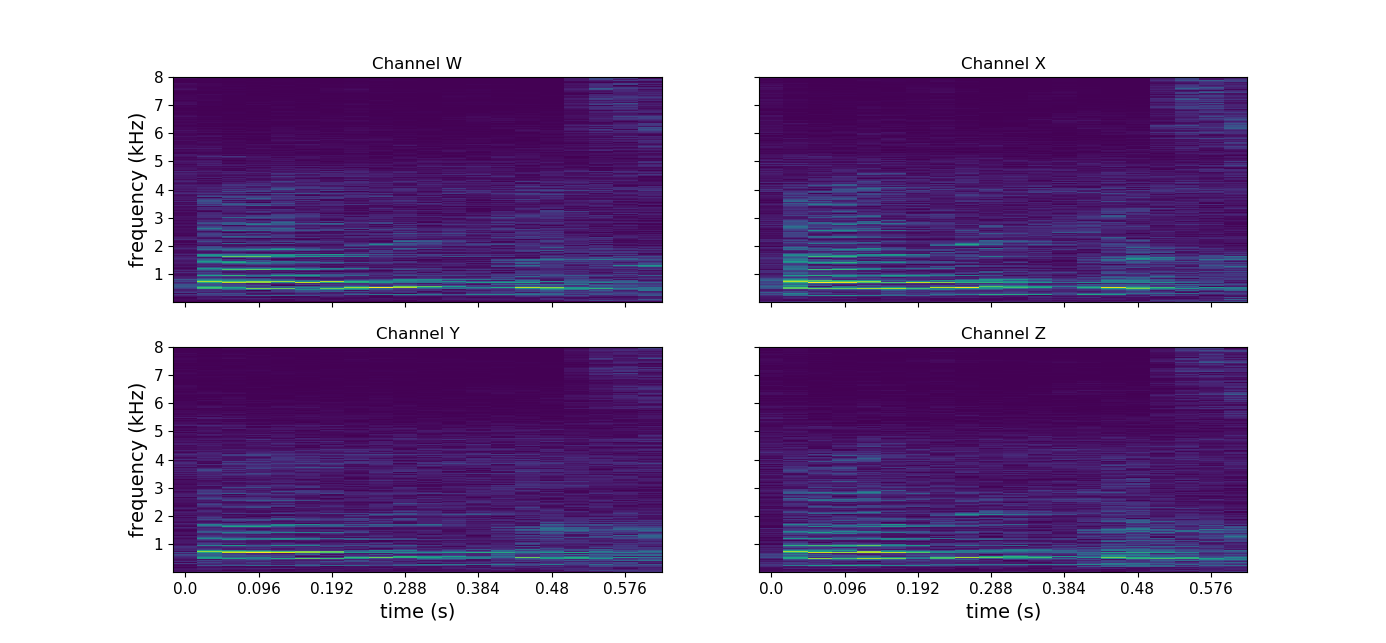
\includegraphics[width=1.\linewidth]{Images/chap5/foaMagnitudeSpectrograms.png}
    \captionof{figure}[Example of an input signal represented with a FOA magnitude spectrogram]{Example of an input signal represented with a FOA magnitude spectrogram. In this example, $T = 20$, and the number of speakers (which is difficult to estimate visually) is $1$ from $0$ to $0.372$~s and $2$ for the remaining frames. For a better visualization, we apply a log function to these spectrograms, but in practice it is not done during the experiments.}
    \label{fig:foaMagnitudeSpectrograms}
    \end{center}
\end{figure}

As it is usual in deep learning, we normalize these spectrograms per frequency band over the entire training dataset, so that the mean and variance for each frequency band (including all frames and channels) are $0$ and $1$, respectively. The same mean and variance values from the training dataset are used to normalize the test data.

\subsection{Speaker counting as a classification problem}

We consider speaker counting as a multi-class classification problem, as it was shown to be more efficient than regression \cite{stoter_classification_2018}. Each class represents a number of speakers, and the network is trained to evaluate the probability of the input feature to belong to that class. More specifically, we limit our speaker counting system to count between $0$ and $5$ speakers, leading to $6$ potential classes $c_i$, $i \in \{0,1,2,3,4,5\}$. Then, for each input frame, the neural network is trained to estimate the probability $P(t,c_i \mid \mathbf{X})$ that the $t$-frame belongs to class $c_i$, and for $i \in \{0,1,2,3,4,5\}$ (\emph{i.e.}, it output $6$ values in $[0,1]$), as illustrated in Fig.~\ref{fig:countingClassification}. As detailed further, we design the network output layer so that all outputs sum to $1$, acting as a discrete probability distribution. Finally, the number of speakers for the considered frame is estimated by selecting the class with the highest probability:
\begin{equation}
    \hat{J}(t) = \argmax_i P(t,c_i \mid \mathbf{X}).
\end{equation}
 
\begin{figure}[t]
    \begin{center}
    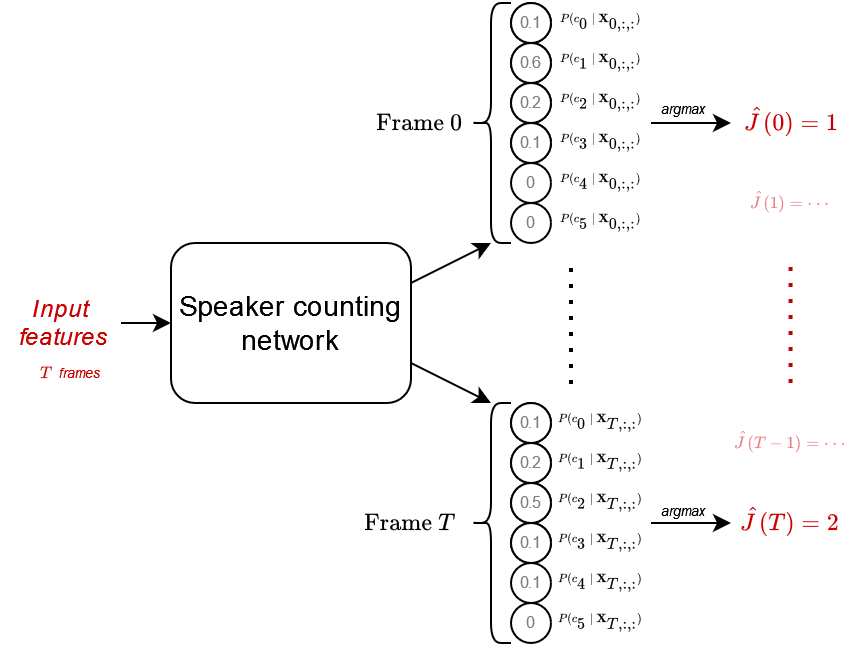
\includegraphics[width=0.9\linewidth]{Images/chap5/countingClassification.png}
    \captionof{figure}[Speaker counting as a classification problem]{Speaker counting as a classification problem. Each candidate number of speakers is considered as a class, and the neural network is trained to estimate the probability that the input feature belongs to each class. The neural network is forced to output the set of probabilities for each frame in the input feature.}
    \label{fig:countingClassification}
    \end{center}
\end{figure}

Note that in our method, a probability for each class is computed for each frame, leading to a frame-wise resolution for our counting system. This is the main difference with \cite{stoter_classification_2018}, in which the authors proposed to calculate a single probability distribution for the whole $5$-s long input sequence.

\subsection{Neural network global architecture}
\label{ss:countingNetworkArchitecture}

The neural network architecture we adopt for speaker counting is inspired by \cite{stoter_countnet:_2019}, and is illustrated on Fig.~\ref{fig:countingNetworkArchitecture}.

A first series of convolutional layers processes the input tensor of shape $T \times 513 \times 4$ (the value $513$, which is the number of frequency bins, comes from the chosen STFT analysis window size, see Section~\ref{ss:countingAudioParameters}), where $T$ is an hyperparameter in our experiments, and performs a feature extraction. This convolutional block first consists of two 2D convolutional layers with 64 and 32 convolution kernels of size $K \times K$, respectively, applied on the temporal and frequency axes, where $K$ is another hyperparameter in our experiments. Then, a max-pooling layer with a pooling size of $1 \times 3$ is used, in order to preserve the information along the temporal axis. Next, two other 2D convolutional layers with respectively 128 and 64 convolution kernels of size $K \times K$ are used, followed by another max-pooling layer of size $1 \times 3$. In all convolutional layers, we use a stride of 1 as well as zero-padding in order to preserve the shape of the input tensor. The important change compared to \cite{stoter_countnet:_2019} is that we use a max-pooling $1 \times 3$ instead of $3 \times 3$, allowing us to preserve the temporal dimension for a prediction at a frame-wise resolution.

The new features extracted by the convolutional module consist of $64$ feature maps of size $T \times 57$. In order to proceed to a temporal analysis with recurrent layers, we reshape the obtained feature by stacking the feature maps along its second dimension, leading to a reshaped feature of size $T \times 3648$. In all convolutional layers, ReLU activations are used. Batch normalization is also applied before each max-pooling layer to make the neural network faster and more stable.

The temporal processing is then done using a single LSTM layer with a hidden state vector size of $40$. This LSTM layer is used in a sequence-to-sequence mode, \emph{i.e.}, the hidden state of the LSTM cell is output at each timestep, so that we obtain a new vector for each item of the input sequence (which is of length $T$). The activation functions used in the LSTM cells are the same as described in Section~\ref{ss:lstm}, \emph{i.e.}, $\sigma_h$ is the hyperbolic tangent function and $\sigma_s$ is the sigmoid function.

Finally, each vector from the output sequence of the LSTM layer is processed independently by the 6-neuron output feedforward layer, whose activation is set to the softmax function. This ensures that a probability distribution over the $6$ classes is produced for each timestep.

\begin{figure}[t]
    \begin{center}
    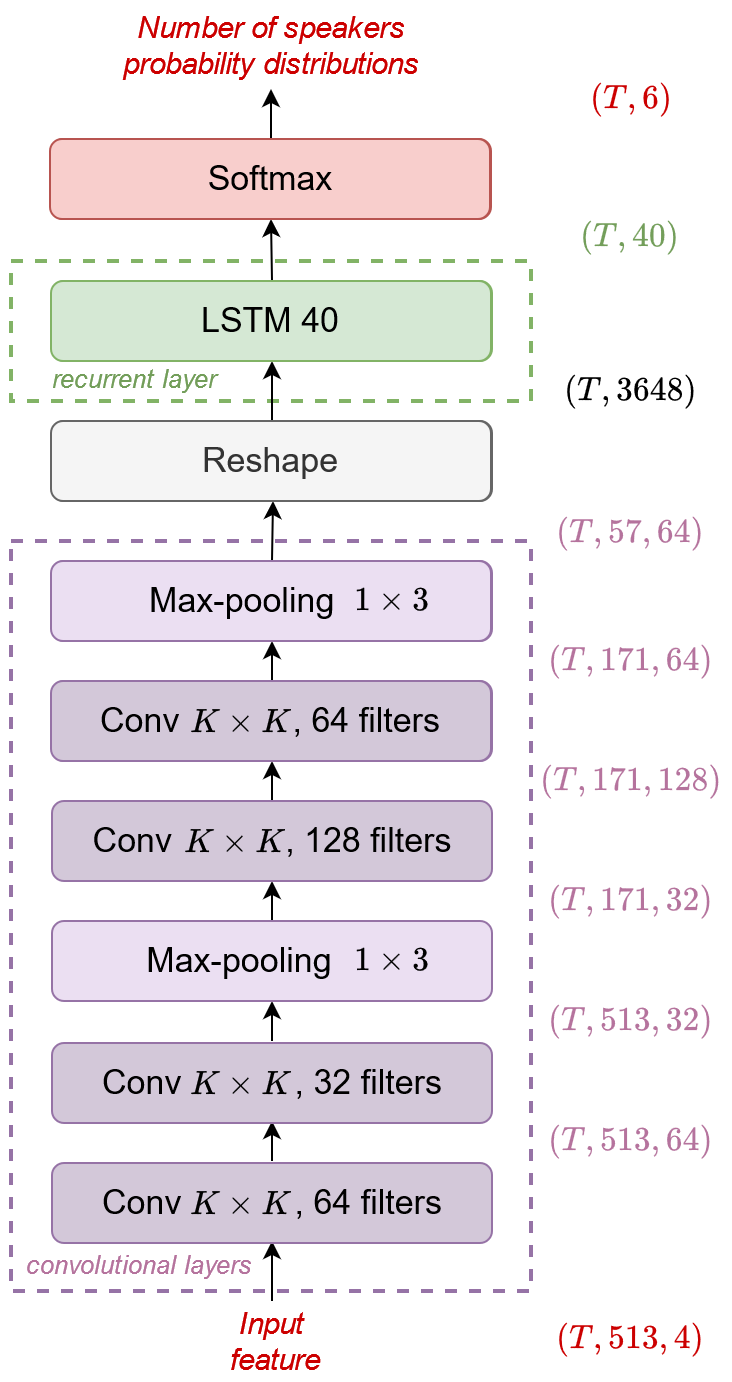
\includegraphics[width=0.4\linewidth]{Images/chap5/countingNetworkArchitecture.png}
    \captionof{figure}[Neural network architecture for speaker counting]{Neural network architecture for speaker counting. It is composed of a series of 2D convolutional layers, with max-pooling layers in-between, followed by an LSTM layer and a feedforward layer acting as the output layer. Max-pooling is applied only on the second axis (corresponding to the frequency dimension) to preserve temporal dimensionality and the LSTM is used in a sequence-to-sequence mode. The convolution kernel size $K \times K$ and the number of frames $T$ in the input features are hyperparameters in our experiments.}
    \label{fig:countingNetworkArchitecture}
    \end{center}
\end{figure}

%-----------------------------------------------
%  EXPERIMENTAL PROTOCOL
%-----------------------------------------------
\section{Experimental protocol}
\subsection{Audio parameters}
\label{ss:countingAudioParameters}

In our experiments, the audio signals are sampled at $16$~kHz, which is the frequency range of the Eigenmike\textsuperscript{\textregistered} array for which the FOA channels exhibit acceptable directivity distortion \cite{baque_analyse_2017}. The STFT is computed using a sinusoidal window of length $1\,024$ ($64$~ms) with an overlap of $50$\%, thus a frame is computed every $32$~ms. The FFT size is also $1\,024$, leading to $513$ frequency bins. 

\subsection{Training parameters}

The loss function used for training is the categorical cross-entropy. The Adam optimizer \cite{kingma_adam:_2014} is used with a starting learning rate of $10^{-3}$, $\beta_1 = 0.9$, $\beta_2=0.999$, $\epsilon = 10^{-7}$. During the training phase, a dropout is used before the reshape layer, with a dropout rate of $0.25$. During training, we monitor the categorical accuracy on the validation set, and we stop the training if the accuracy has not improved for $20$ epochs, keeping the model with the best accuracy so far. The maximum number of epochs is set to $300$. When the validation accuracy has not improved for 10 epochs, we divide the learning rate by a factor $2$.

\subsection{Training data}
\label{ss:countingTrainingData}

Our speaker counting CRNN is trained on simulated data. The simulation can be decomposed into two phases: the generation of RIRs and the generation of the training signals.

The RIRs are simulated with the image-source method \cite{allen_image_1979}, by adapting an existing framework \cite{habets_room_2006} to generate FOA RIRs. A large number of RIRs are generated in a variety of random conditions, such as the room dimensions and absorption coefficients, the microphone and source positions. First, we randomly set the dimension of the room, which is simplified to be parallelepipedic (usually referred to as a \textit{shoebox}), within $[2,10]$~m, $[2,10]$~m and $[2,3]$~m, for the length, width and height, respectively. The room RT60 is randomly chosen between $200$ and $800$~ms. Next, an ideal (open sphere) spherical microphone is randomly positioned in the room so that it is at least at a distance of $0.5$~m from the walls. Then, $5$ source positions are randomly picked within the room dimensions. The protocol is repeated for $10\,000$ rooms, so that we end up with $50\,000$ RIRs.

To generate the speech mixtures, we use $16$-kHz speech excerpts from the TIMIT dataset \cite{garofolo_timit_1993}. To match realistic conditions, we want to generate conversation-like mixtures, with the instantaneous number of speakers (in between $0$ and $5$) varying over time. The speech mixtures also need to be generated as if the speakers were in the same room (hence the $5$ generated RIRs per room). To create such a realistic signal, we first fix a total number of speakers $J$ which will participate in the current speech mixture (between $1$ and $5$). To create the mixture, a single-speaker $15$~s dry signal is first generated by concatenating several sentences from a unique random speaker in the TIMIT database (it is crucial in this step not to mix sentences from different speakers to ensure the continuity of one speaker's frequency content) and alternating actual speech content with silence segments. More specifically, a preliminary silence with a random length in $[0.5,1]$~s first initializes the signal. Then a random sentence from the chosen speaker is concatenated with the signal, followed by a silence of random length in $[0.5,2]$~s. This last step is repeated for random sentences until a $15$~s signal is obtained.\footnote{If the last concatenated sentence is too long so that the signal will be longer than $15$~s, it is cropped and faded out in the last $100$~ms.} The obtained single-speaker $15$~s dry signal is then convolved with one RIR of a randomly picked room to create a wet signal. This process is repeated for the $J$ speakers of the current mixture, using the $J$ distinct RIRs from the same room. Then, we mix all the single-speaker wet signals together to create a speech mixture with an instantaneous number of speakers varying from $0$ to $J$ speakers. The signal-to-interference ratios (SIR) used between the first single-speaker signal and the other signals is randomly chosen in $[0,10]$~dB. The last step is to add a diffuse noise to this mixture to make it a step further more realistic. We randomly choose a noise signal among those in a noise database constituted from various signals from Freesound\footnote{https://freesound.org/} (including crowd, traffic, engine, nature sounds, etc.), which we convolve with a diffuse field generated by averaging the diffuse parts of two random RIRs measured in a real reverberant room. A random SNR is picked in $[0,20]$~dB with respect to the first speech signal.

In the TIMIT dataset, each speech sentence is annotated with the pronounced word timestamps, at a sample precision. We use these annotations to automatically label voice activity vs silence for each speaker and thus label the $15$~s mixtures with the ground-truth number of speakers at the sample resolution. When these signals are transformed into the STFT domain, we consider that a speaker is active in a frame if it is active for more than half of the samples in that frame.

Fig.~\ref{fig:spectrogramsWithVaryingNOS} illustrates three examples of a $15$~s mixture with a varying number of speakers. Because each speaker randomly starts and stops uttering small sentences, the number of speakers varies several times along the sequence.

\begin{figure}[t]
    \begin{center}
    \makebox[\textwidth][c]{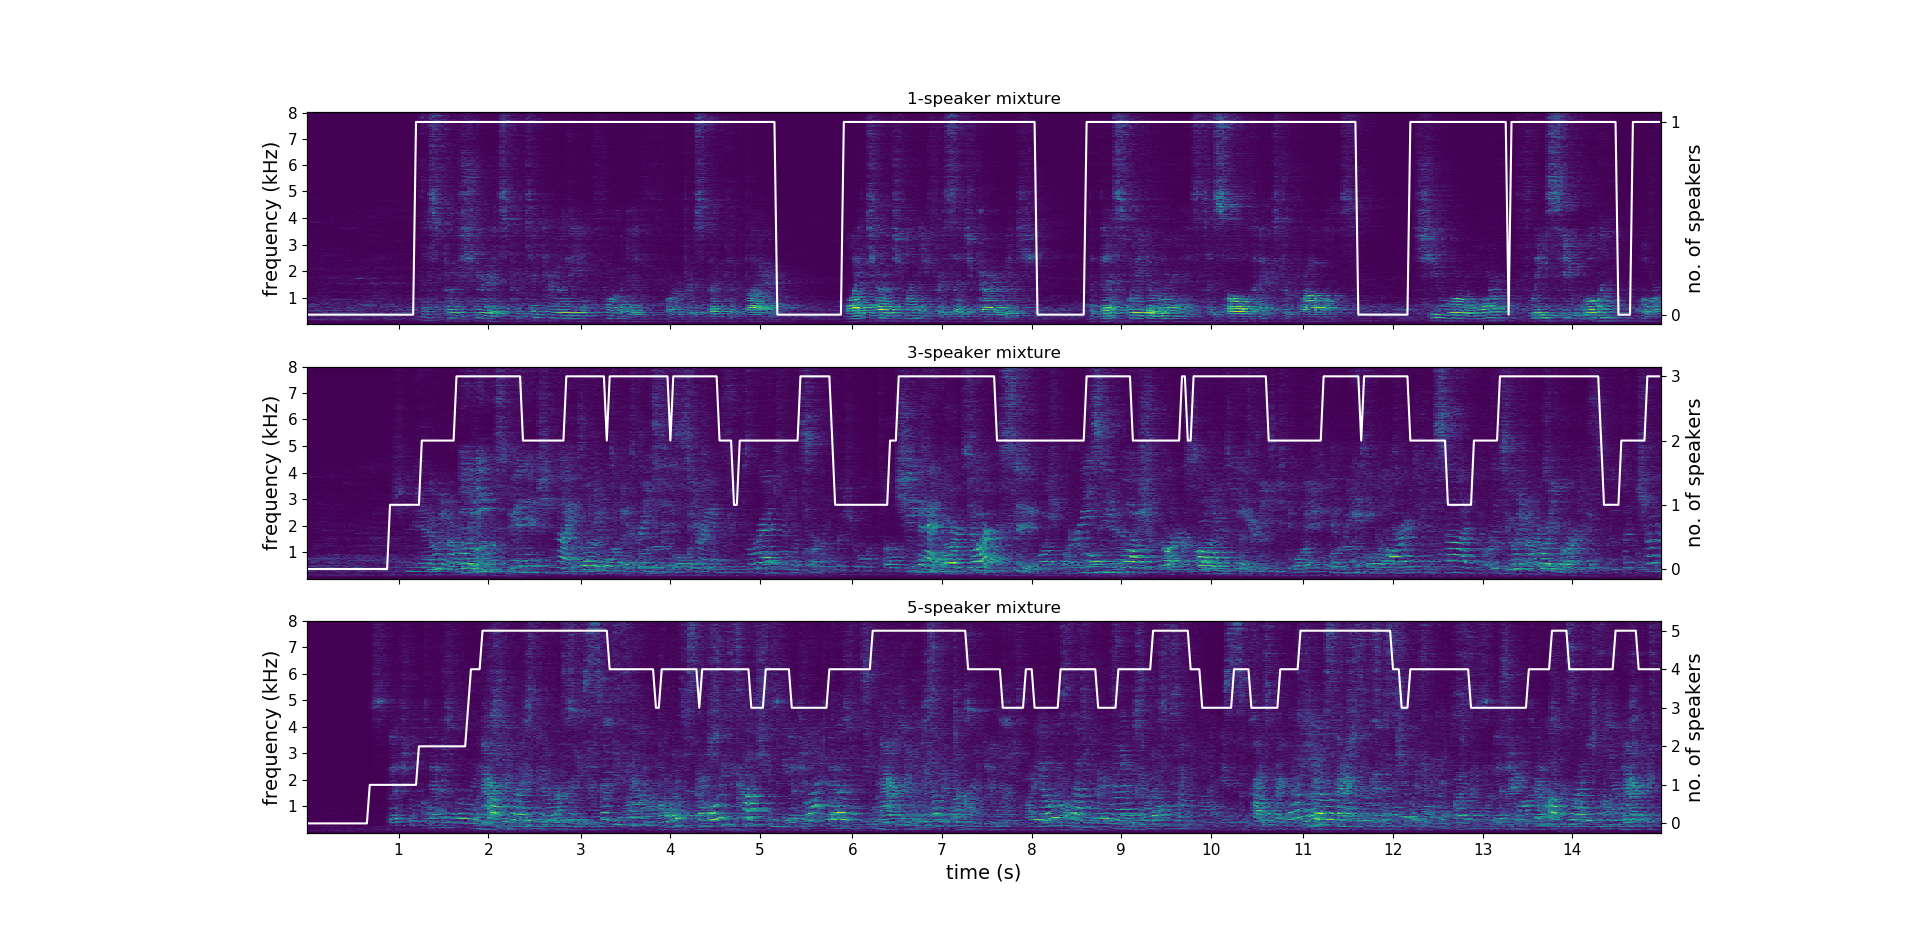
\includegraphics[width=1.4\linewidth]{Images/chap5/spectrogramsWithVaryingNOS.png}}
    \captionof{figure}[Example of spectrograms of $15$~s long signals with varying number of speakers]{Example of spectrograms ($W$ channel only) of $15$~s long training signals with varying number of speakers. The white lines represent the varying (ground-truth) number of speakers in each mixture. The maximum number of speakers in these mixture are $1$ (top), $3$ (middle) and $5$ (bottom). As we can see, the instantaneous number of speakers ``continuously'' varies along the $15$~s of mixture, as each speaker starts and stops uttering a small sentence all along the signal.}
    \label{fig:spectrogramsWithVaryingNOS}
    \end{center}
\end{figure}

We recall that each (train or test) input feature to our network is a sequence of $T$ consecutive 4-channel FOA STFT magnitude frames, with $T$ an hyperparameter that we set experimentally. These sequences are extracted from these $15$~s mixtures with basic segmentation, without any overlap between the sequences.
The first version of our training dataset consisted of 5 $J$-speaker $15$-s mixtures, for $J \in \{1,2,3,4,5\}$, for each room, leading to the same number of training/test sequences for each number of speaker $J$. However this strategy actually raises the famous \textit{class imbalance problem} \cite{buda_systematic_2018}, which happens when the number of examples is very different for each class. As we can see in the plots on Fig.~\ref{fig:spectrogramsWithVaryingNOS}, in each mixture the instantaneous number of speakers fluctuates around certain values and rarely reaches others. For example, in the $3$-speaker mixture, the number of speakers is most often $2$ or $3$, while in the bottom plot we see that there barely are $5$-speaker frames. Globally, generating the exact same number of $J$-speaker mixtures for all values of $J$ would unbalance the cardinality of each class, with more training data towards the low-valued classes. To avoid this problem, we decide not to systematically generate all $5$ speech mixtures for each room, but rather setting a probability that a $J$-speaker mixture will actually be generated. Table~\ref{tab:NOSgenerationProbabilities} shows these probabilities, set empirically to attain a more balanced training dataset. To illustrate this process, let us assume we already selected a certain room configuration, which comes with $5$ generated SRIRs. We first consider a $1$-speaker mixture, which probability of generation is $0.2$ as indicated in Table~\ref{tab:NOSgenerationProbabilities}. Whether the draw leads to the actual mixture generation or not, we then consider the generation of a $2$-speaker mixture, this time with a probability of $0.3$. We continue in this process until considering the generation of a $5$-speaker mixture, which is actually always done because of the probability $1$. In that manner, we have actually generated $1$-speaker mixtures using $1$ SRIR from only $20$\% of the considered rooms, $2$-speaker mixtures using $2$ SRIRs from only $30$\% of the rooms, etc.


\begin{table}[t]
\centering
\begin{tabular}{|c|ccccc|}
\hline
\textbf{$J$}                                                                                                      & \textbf{1}           & \textbf{2}           & \textbf{3}           & \textbf{4}           & \textbf{5}         \\ \hline
\multirow{2}{*}{\textbf{\begin{tabular}[c]{@{}c@{}}Probability to generate\\ a $J$-speaker mixture\end{tabular}}} & \multirow{2}{*}{0.2} & \multirow{2}{*}{0.3} & \multirow{2}{*}{0.4} & \multirow{2}{*}{0.5} & \multirow{2}{*}{1} \\
                                                                                                                  &                      &                      &                      &                      &                    \\ \hline
\end{tabular}
\captionof{table}[Probabilities of generating a $J$-speaker mixture]{Probabilities of generating a $J$-speaker mixture during the creation of the training dataset.}
\label{tab:NOSgenerationProbabilities}
\end{table}

The validation dataset, used to monitor the neural network training, is created exactly with the same methodology. Only $100$ rooms are considered for this dataset, and we took care not to use generation data already used for the training dataset (speech sentences, speaker identities, rooms, noise signals).

Finally, we end up with about $100$~hours of training data and $1$~hour of validation data.

\subsection{Testing data}
\label{ss:countingTestingData}

The test dataset used to assess our models is a simulated dataset created in the same manner as the training and validation datasets. For the test, we generated $500$ RIRs in $100$ different rooms. Again, the speakers and noise signals used for the test signals have not been used for the training and validation datasets. The obtained test dataset contains $1$~hour of data. 

\subsection{Baseline}

As our speaker counting system is partly inspired by the classification-based CRNN proposed in \cite{stoter_countnet:_2019}, we consider this method as a baseline for the experiment in which we compare the use of single- and multi-channel signals. We nevertheless adjust this baseline to ensure having a fair comparison to our method. First, we employ the recurrent layer in a sequence-to-sequence manner so that a prediction is made for every frame in the input feature.\footnote{In \cite{stoter_countnet:_2019}, the authors designed their network to produce only one prediction for the whole input feature, as their goal was to predict the maximum number of speakers present in a $5$-s single-channel mixture.} This choice constraints us to use max-pooling of size $1 \times 3$ instead of $3 \times 3$ to preserve the temporal dimension.


\subsection{Evaluation metrics}

To measure the performance of our speaker counting system we use several metrics. The classification accuracy $A_{ii}$ for one class $c_i$ is defined by the percentage of frames correctly classified with class $c_i$, among all frames belonging to class $c_i$. While it is a usual metric in a classification problem, we also extend this metric to measure the percentage of frames that are classified with class $c_j$ among all frames belonging to class $c_i$. Hereafter, $A$ is referred as the confusion matrix. Mathematically, by noting $T_i$ the set of all test frames indices with the ground-truth number of speakers equal to $i$, $A_{ij}$ is expressed as:
\begin{equation}
    A_{ij} = \frac{\mathsf{card}(\{t \in T_i \mid \hat{J}(t) = j\})}{\mathsf{card}(T_i)},
\end{equation}
where $\mathsf{card}(T_i)$ denotes the cardinality of the set $T_i$.
This accuracy metric calculated according to two indices (each representing a NoS) will be useful to assess how far the estimated number of speakers deviates from the ground-truth value. 

We also measure the mean absolute error $M_i$ per class, which is defined as:
\begin{equation}
    M_i = \frac{1}{\mathsf{card}(T_i)} \sum_{t \in T_i} \lvert \hat{J}(t) - J(t) \rvert.
\end{equation}

%-----------------------------------------------
%  EXPERIMENTS
%-----------------------------------------------
\section{Experiments}

In this section, we report and discuss the results of our speaker counting CRNN evaluation. We conduct several experiments in which we assess the values of some hyperparameters: the benefit of using multi-channel signals, the number of frames in the input sequence, the convolution kernel sizes. We also propose an analysis of the accuracy of the network depending on the frame position within the input sequence.

\subsection{Single-channel against multi-channel features, with several sequence lengths}

\subsubsection{Experiment objective}

The preliminary objective of our speaking counting CRNN is to assess the benefit of using multi-channel signals over single-channel ones, such as the one proposed in \cite{stoter_countnet:_2019}. As explained above, we adapt this baseline network to our problem of estimating the instantaneous number of speakers. Therefore, the baseline in this experiment is the same speaker counting architecture we adopt, presented in Section~\ref{ss:countingNetworkArchitecture}, but we limit the input features to only one channel. Instead of using the $4$ channels obtained from the FOA representation, only the $W$ channel is considered for the baseline. The $W$ channel encodes the recorded signal as if it was recorded by an omnidirectional microphone, which can be adequately considered as a single-channel representation. 

\begin{figure}[t]
    \centering
    \makebox[\textwidth][c]{
    \subfloat[Single-channel,\\ 10 frames]{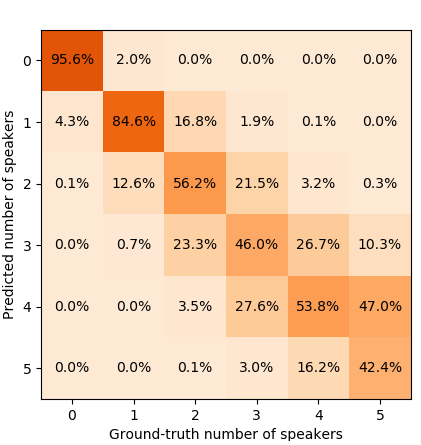
\includegraphics[width=.4\textwidth]{Images/chap5/conf_mat_mono_10frames_simulatedSRIRs.png} \label{subfig:cm_mono_10frames_sim}}
    \subfloat[Single-channel,\\ 20 frames]{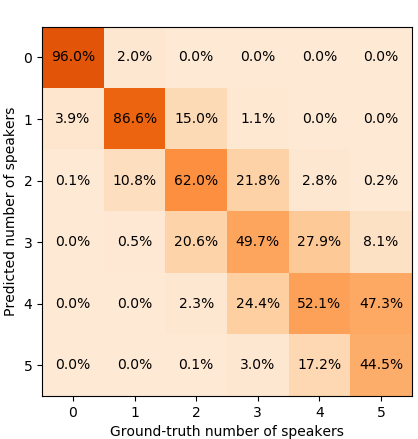
\includegraphics[width=.4\textwidth]{Images/chap5/conf_mat_mono_20frames_simulatedSRIRs.png} \label{subfig:cm_mono_20frames_sim}}
    \subfloat[Single-channel,\\ 30 frames]{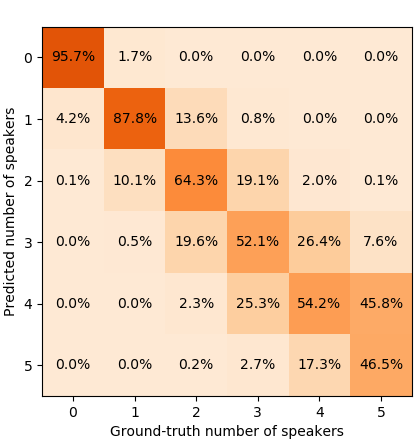
\includegraphics[width=.4\textwidth]{Images/chap5/conf_mat_mono_30frames_simulatedSRIRs.png} \label{subfig:cm_mono_30frames_sim}}}\\
    
    \makebox[\textwidth][c]{
    \subfloat[Multi-channel,\\ 10 frames]{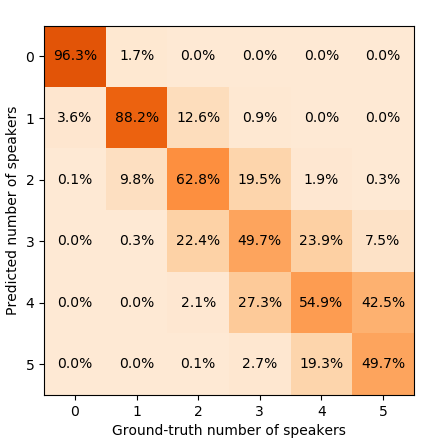
\includegraphics[width=.4\textwidth]{Images/chap5/conf_mat_multi_10frames_simulatedSRIRs.png} \label{subfig:cm_multi_10frames_sim}}
    \subfloat[Multi-channel,\\ 20 frames]{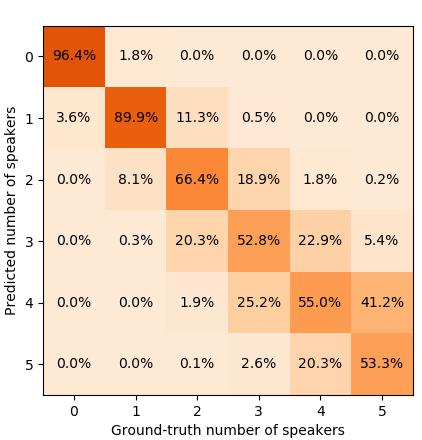
\includegraphics[width=.4\textwidth]{Images/chap5/conf_mat_multi_20frames_simulatedSRIRs.png} \label{subfig:cm_multi_20frames_sim}}
    \subfloat[Multi-channel,\\ 30 frames]{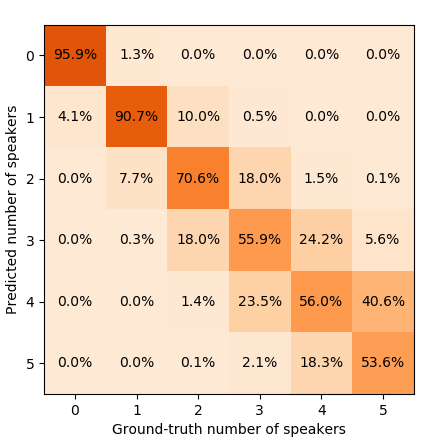
\includegraphics[width=.4\textwidth]{Images/chap5/conf_mat_multi_30frames_simulatedSRIRs.png} \label{subfig:cm_multi_30frames_sim}}}
    
    \captionof{figure}[Confusion matrix $A_{ij}$ of the single-channel and multi-channel speaker counting CRNNs on the test dataset with simulated SRIRs, for several values of $T$]{Confusion matrix $A_{ij}$ of the single-channel (top) and multi-channel (bottom) speaker counting CRNNs on the test dataset with simulated SRIRs, for $T = 10, 20, 30$~frames (left to right).}
    \label{fig:confusionMatricesSingleMultiSimulated}
\end{figure}

The intuition behind using multi-channel features is to provide the neural network with a means to better discriminate between spatially distinct sources. As it is done in source localization (see Chapter~\ref{chap:multisourceLocalization}), feeding multi-channel features to the neural network supplies it with multiple transformed versions of the same signal (due to the different microphone types and orientations). Depending on the source location, the original signal is not transformed the same way, which should be reflected in the magnitude spectrogram. We conjecture that the neural network can learn these characteristics to better discriminate the different speech sources.

To compare the use of single- and multi-channel features in several conditions, we also vary the length of the input sequence, \emph{i.e.}, the number of frames $T$ in the input features. We experimented with $T=10$ ($320$~ms), $T=20$ ($640$~ms), and $T=30$ ($\approx 1$~s). In this experiment, the convolution kernel size is $K=3$ (see Section~\ref{ss:countingConvolutionExperiment} for an experiment on this hyperparameter).

\subsubsection{Results}

\begin{figure}[t]
    \centering
    \makebox[\textwidth][c]{
    \subfloat[Single-channel,\\ 10 frames]{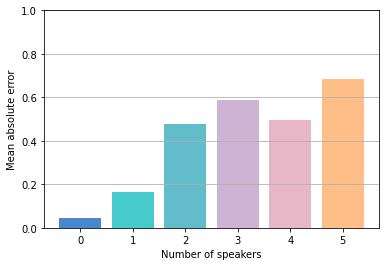
\includegraphics[width=.4\textwidth]{Images/chap5/mae_mono_10frames_simulatedSRIRs.png} \label{subfig:mae_mono_10frames_sim}}
    \subfloat[Single-channel,\\ 20 frames]{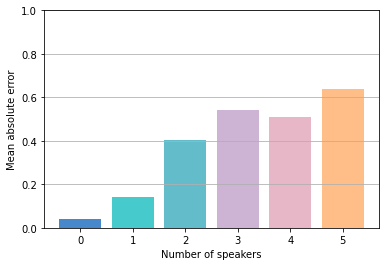
\includegraphics[width=.4\textwidth]{Images/chap5/mae_mono_20frames_simulatedSRIRs.png} \label{subfig:mae_mono_20frames_sim}}
    \subfloat[Single-channel,\\ 30 frames]{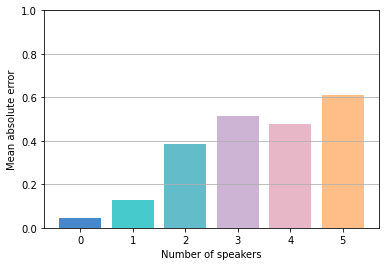
\includegraphics[width=.4\textwidth]{Images/chap5/mae_mono_30frames_simulatedSRIRs.png} \label{subfig:mae_mono_30frames_sim}}}\\
    
    \makebox[\textwidth][c]{
    \subfloat[Multi-channel,\\ 10 frames]{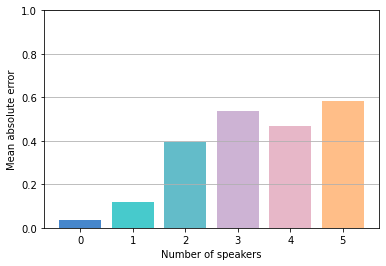
\includegraphics[width=.4\textwidth]{Images/chap5/mae_multi_10frames_simulatedSRIRs.png} \label{subfig:mae_multi_10frames_sim}}
    \subfloat[Multi-channel,\\ 20 frames]{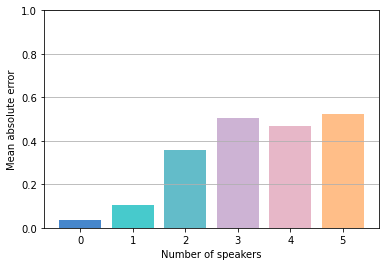
\includegraphics[width=.4\textwidth]{Images/chap5/mae_multi_20frames_simulatedSRIRs.png} \label{subfig:mae_multi_20frames_sim}}
    \subfloat[Multi-channel,\\ 30 frames]{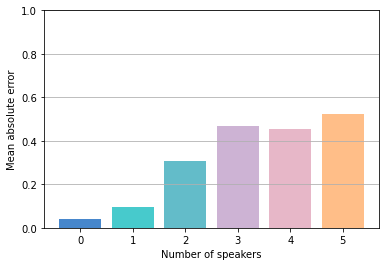
\includegraphics[width=.4\textwidth]{Images/chap5/mae_multi_30frames_simulatedSRIRs.png} \label{subfig:mae_multi_30frames_sim}}}
    
    \captionof{figure}[Mean absolute errors $M_i$ of the single-channel and multi-channel speaker counting CRNNs on the test dataset with simulated SRIRs, for several values of $T$]{Mean absolute errors $M_i$ of the single-channel and multi-channel speaker counting CRNNs on the test dataset with simulated SRIRs, for $T = 10, 20, 30$~frames (left to right).}
    \label{fig:maeSingleMultiSimulated}
\end{figure}


We report the detailed accuracy results for all $6$ experiments in the form of confusion matrices, which display the percentage of $j$-speaker frames (on the x-axis) which are estimated to contain $j$ speakers (on the y-axis). These confusion matrices are shown in Figure~\ref{fig:confusionMatricesSingleMultiSimulated}. We also report graphics of the mean absolute errors in Figure~\ref{fig:maeSingleMultiSimulated}. We recall that we compare the use of single-channel features to multi-channel features, for $3$ values of $T$: $10$, $20$ and $30$ frames.

First, we notice that both single- and multi-channel networks are very effective to detect the absence of speech in the signal, with over $95$\% of correct silent detection in all settings. It can therefore act as a robust VAD system. Then, the classification accuracy gradually decreases when the number of speakers increases, which is anticipated since the task becomes more complex. While the classification accuracy for $1$-speaker signals is around $85$\% for the single-channel network, it reaches around $44$\% accuracy when $5$ speakers are present in the signal, which is still an acceptable performance compared to a random guessing accuracy ($16$\%). 

While the mean absolute error is almost zero for zero-speaker signals in all configurations, it remains under $0.8$ when one or more speakers are active, which means that when the neural network predicts a wrong number of speakers, the error is $\pm 1$ speaker in average. This behavior can be clearly noticed in the confusion matrices. When the network's prediction is wrong it is almost always done with an absolute error of $1$, which is visualized around the matrix diagonal. For example, in Fig.~\ref{subfig:cm_multi_20frames_sim}, we see that when the ground-truth number of speakers is $3$, the neural network predicts wrongly $2$ speakers $18.9$\% of the time and $4$ speakers $25.2$\%, while it estimates $0$, $1$ or $5$ only $3.1$\% of the time in total. Regarding the class $J=5$ speakers, there seems to be an \textit{edge effect}, so that the number of prediction for $J-1$ speakers is surprisingly high compared to the other values of $J$, but this can be explained because of the absence of the class $J=6$.

When comparing the effectiveness of the single- and multi-channel settings, we clearly see an increase in accuracy when multiple channels are taken into account, for all values of $T$. The gain in accuracy of the multi-channel network becomes larger when the number of speakers increases. We see in Fig.~\ref{fig:confusionMatricesSingleMultiSimulated} that, when $T=10$, the accuracy goes from $84.6$\% to $88.2$\% for $1$-speaker signals ($\approx 4$\% gain), from $46.0$\% to $49.7$\% for $3$-speaker signals ($\approx 8$\% gain) and from $42.4$\% to $49.7$\% for $5$-speaker signals ($\approx 17$\% gain). When $T=30$, the accuracy goes from $87.8$\% to $90.7$\% for $1$-speaker signals ($\approx 3$\% gain), from $52.1$\% to $55.9$\% for $3$-speaker signals ($\approx 7$\% gain) and from $46.5$\% to $53.6$\% for $5$-speaker signals ($\approx 15$\% gain). These gains seem to confirm our preliminary conjecture which stated that the neural network takes benefit of the spatial characteristics present in the input multi-channel magnitude spectrogram, because the source locations are distinct enough. When looking at Fig.~\ref{fig:maeSingleMultiSimulated}, we also notice an improvement in terms of mean absolute error for all multi-channel settings.

Regarding the input sequence length $T$, we notice that the more frames in the spectrogram, the more accurate is the neural network. It also seems to confirm our intuition that more temporal context is benefit for the neural network since it can process more successive frames. Due to how we generated our dataset, with simulated conversation-like signals, each frame has a number of speakers close to that of the neighboring frames: it is often the same number of speakers, sometimes it is shifted by $\pm 1$ speaker. As we will see in more details in Section~\ref{ss:accuracyAlongTheSequence}, another important factor to explain this gain in accuracy when $T$ is larger is the nature of the LSTM layer to process past data to improve its prediction. 

Finally, we can conclude that the multi-channel CRNN surpasses the single-channel model in all configurations, showing the usefulness of a multi-microphone inputs. The multi-channel CRNN is able to predict the instantaneous number of speakers of simulated data with an accuracy of at least $50$\% for all NoS, even with a short signal snapshot ($320$~ms), which is very interesting for online systems.

\subsection{Convolution kernel sizes}
\label{ss:countingConvolutionExperiment}
\subsubsection{Experiment objective}

Now that we have demonstrated the benefit of the spatial information for speaker counting, we explore how the neural network performance varies when we change other parameters. In particular, in this experiment, we analyse the performance of the neural network as a function of the size of the convolution kernels. We have tested the increase of the kernel size from $3 \times 3$, as employed in the previous series of experiments, to $5 \times 5$ and $7 \times 7$. The goal is to make the convolutions span over more values during the feature extraction step, and see if it can provide the network a more flexible way to process the temporal and frequency dimensions.

\subsubsection{Results}

The confusion matrices and mean absolute error plots obtained from this new experiment are shown in Fig.~\ref{fig:confusionMatricesKernelSizes} and \ref{fig:maeKernelSizes}, respectively. The first remark is that the same effect can be observed regarding the length of the input sequence, that is the speaker counting accuracy increases when $T$ gets larger.

Regarding the evolution of the performance according to the size of the convolution kernels, it seems that the overall accuracy is higher when the kernel size increases, although it decreases for some values. To give some numbers, for $T=10$, $A_{55}$ is $49.7$\% for $K=3$ whereas it reaches $58.6$\% for $K=7$. However, for $T=20$, $A_{55}$ is equal to $53.3$\% for $K=3$, largely increases to $63.4$\% for $K=5$ but falls down to $53.0$\% for $K=7$. Due to the fluctuations of the evolution of $A_{ij}$ it is not straightforward to conclude with the confusion matrices. It is more apparent when looking at the mean absolute error plots on Fig.~\ref{fig:maeKernelSizes}, where we see that the mean absolute error decreases in almost all cases when the kernel size expands. It is a bit more noticeable for higher number of speakers.

It thus seems that the neural network benefits, to some extent, from a larger span over the frames and frequency bins. Regarding the frequency dimension, one can think that the feature extraction with larger kernels would help the network to better gather the frequency content of distinct speakers. On the temporal axis, it can be beneficial to have access to more past or future frames in order to integrate the frequency content of several speakers with respect to time. This can be even more advantageous due to the intermittent nature of speech, however it is not clear if this has more to do with the LSTM layer than the other network's components. 

To conclude this experiment, we see that the expansion of the convolution kernel helps increasing the accuracy of the counting network, although the gain is quite limited. An explanation of this increase could be that the network is able to access more frequency and temporal contents during the feature extraction, which can be beneficial to better weight the respective contribution of each speaker in the input features.

\begin{figure}[t]
    \centering
    \makebox[\textwidth][c]{
    \subfloat[Kernels $3 \times 3$,\\ 10 frames]{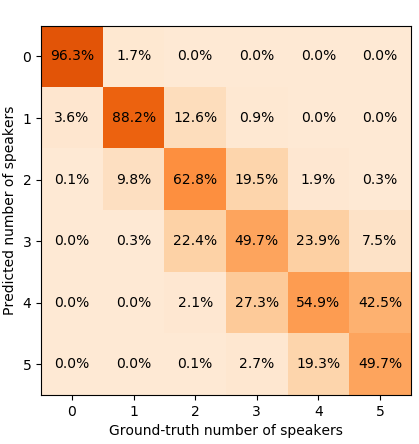
\includegraphics[width=.4\textwidth]{Images/chap5/conf_mat_3_3_10frames_simulatedSRIRs.png} \label{subfig:cm_3_3_10frames}}
    \subfloat[Kernels $3 \times 3$,\\ 20 frames]{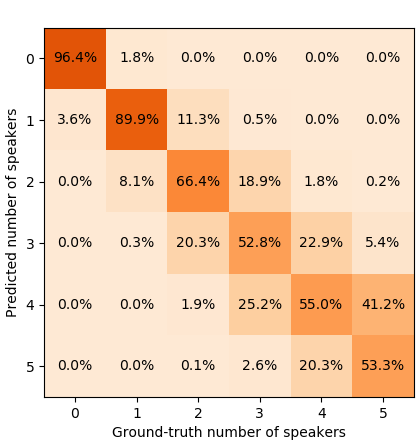
\includegraphics[width=.4\textwidth]{Images/chap5/conf_mat_3_3_20frames_simulatedSRIRs.png} \label{subfig:cm_3_3_20frames}}
    \subfloat[Kernels $3 \times 3$,\\ 30 frames]{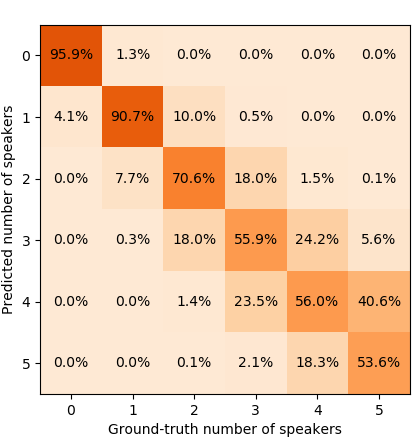
\includegraphics[width=.4\textwidth]{Images/chap5/conf_mat_3_3_30frames_simulatedSRIRs.png} \label{subfig:cm_3_3_30frames}}}\\
    
    \makebox[\textwidth][c]{
    \subfloat[Kernels $5 \times 5$,\\ 10 frames]{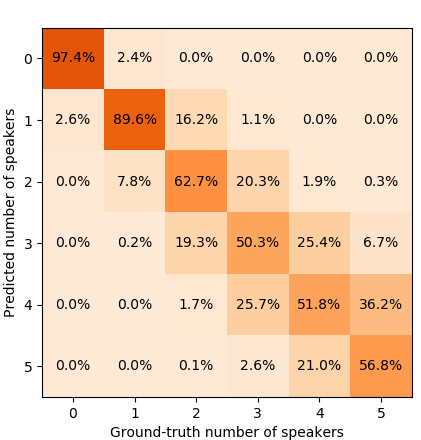
\includegraphics[width=.4\textwidth]{Images/chap5/conf_mat_5_5_10frames_simulatedSRIRs.png} \label{subfig:cm_5_5_10frames}}
    \subfloat[Kernels $5 \times 5$,\\ 20 frames]{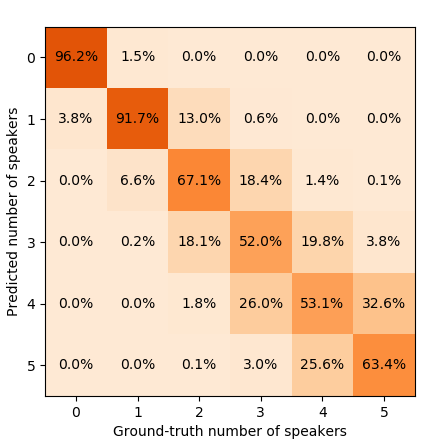
\includegraphics[width=.4\textwidth]{Images/chap5/conf_mat_5_5_20frames_simulatedSRIRs.png} \label{subfig:cm_5_5_20frames}}
    \subfloat[Kernels $5 \times 5$,\\ 30 frames]{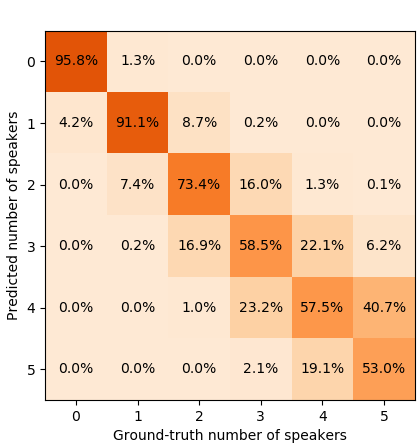
\includegraphics[width=.4\textwidth]{Images/chap5/conf_mat_5_5_30frames_simulatedSRIRs.png} \label{subfig:cm_5_5_30frames}}}\\
    
    \makebox[\textwidth][c]{
    \subfloat[Kernels $7 \times 7$,\\ 10 frames]{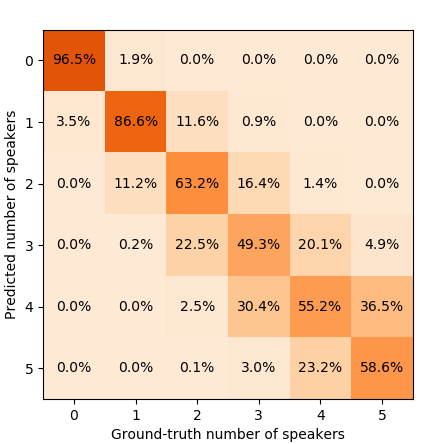
\includegraphics[width=.4\textwidth]{Images/chap5/conf_mat_7_7_10frames_simulatedSRIRs.png} \label{subfig:cm_7_7_10frames}}
    \subfloat[Kernels $7 \times 7$,\\ 20 frames]{\includegraphics[width=.4\textwidth]{Images/chap5/conf_mat_7_7_20frames_simulatedSRIRs.png} \label{subfig:cm_7_7_20frames}}
    \subfloat[Kernels $7 \times 7$,\\ 30 frames]{\includegraphics[width=.4\textwidth]{Images/chap5/conf_mat_7_7_30frames_simulatedSRIRs.png} \label{subfig:cm_7_7_30frames}}}
    
    \captionof{figure}[Confusion matrix $A_{ij}$ of the multi-channel speaker counting CRNN on the test dataset, for several values of $(K \times K)$]{Confusion matrices of the accuracy $A_{ij}$ of the proposed speaker counting multi-channel CRNN, evaluated on the test dataset, for convolution kernels of size $3 \times 3$ (top), $5 \times 5$ (middle row), and $7 \times 7$ (bottom), and for an input sequence length $T=10$ frames (left), $20$ frames (middle column), and $30$ frames (right).}
    \label{fig:confusionMatricesKernelSizes}
\end{figure}

\pagebreak

\begin{figure}[t]
    \centering
    \makebox[\textwidth][c]{
    \subfloat[Kernels $3 \times 3$,\\ 10 frames]{\includegraphics[width=.4\textwidth]{Images/chap5/mae_3_3_10frames_simulatedSRIRs.png} \label{subfig:mae_3_3_10frames}}
    \subfloat[Kernels $3 \times 3$,\\ 20 frames]{\includegraphics[width=.4\textwidth]{Images/chap5/mae_3_3_20frames_simulatedSRIRs.png} \label{subfig:mae_3_3_20frames}}
    \subfloat[Kernels $3 \times 3$,\\ 30 frames]{\includegraphics[width=.4\textwidth]{Images/chap5/mae_3_3_30frames_simulatedSRIRs.png} \label{subfig:mae_3_3_30frames}}}\\
    
    \makebox[\textwidth][c]{
    \subfloat[Kernels $5 \times 5$,\\ 10 frames]{\includegraphics[width=.4\textwidth]{Images/chap5/mae_5_5_10frames_simulatedSRIRs.png} \label{subfig:mae_5_5_10frames}}
    \subfloat[Kernels $5 \times 5$,\\ 20 frames]{\includegraphics[width=.4\textwidth]{Images/chap5/mae_5_5_20frames_simulatedSRIRs.png} \label{subfig:mae_5_5_20frames}}
    \subfloat[Kernels $5 \times 5$,\\ 30 frames]{\includegraphics[width=.4\textwidth]{Images/chap5/mae_5_5_30frames_simulatedSRIRs.png} \label{subfig:mae_5_5_30frames}}}\\
    
    \makebox[\textwidth][c]{
    \subfloat[Kernels $7 \times 7$,\\ 10 frames]{\includegraphics[width=.4\textwidth]{Images/chap5/mae_7_7_10frames_simulatedSRIRs.png} \label{subfig:mae_7_7_10frames}}
    \subfloat[Kernels $7 \times 7$,\\ 20 frames]{\includegraphics[width=.4\textwidth]{Images/chap5/mae_7_7_20frames_simulatedSRIRs.png} \label{subfig:mae_7_7_20frames}}
    \subfloat[Kernels $7 \times 7$,\\ 30 frames]{\includegraphics[width=.4\textwidth]{Images/chap5/mae_7_7_30frames_simulatedSRIRs.png} \label{subfig:mae_7_7_30frames}}}
    
    \captionof{figure}[Mean absolute errors $M_i$ of the multi-channel speaker counting CRNN on the test dataset, for several values of $(K \times K)$]{Mean absolute errors $M_i$ of the multi-channel speaker counting CRNN on the test dataset, for several values of $(K \times K)$.}
    \label{fig:maeKernelSizes}
\end{figure}

\clearpage
\subsection{Counting accuracy profile along the sequence}
\label{ss:accuracyAlongTheSequence}

\subsubsection{Experiment objective}

After analyzing the effect of the sequence length $T$ and noticing that the network performance is better when $T$ increases, we concluded that the LSTM layer makes better predictions if it can rely on more past frames. Moreover, we recall the reader that we use the LSTM in a sequence-to-sequence manner (\emph{i.e.}, the LSTM makes a prediction at each timestep, using the processing of the previous timesteps). Therefore, one can legitimately think that making a prediction in the beginning of the input sequence will generally be less accurate than a prediction at the end of the sequence.

To verify this idea, we measure the overall categorical accuracy $A$ regardless of the class, for an estimate at each frame position in the sequence. This frame-wise accuracy is defined by:
\begin{equation}
    \label{eq:overallCountingCategoricalAccuracy}
    A(\tau) = \frac{\sum_{i=0}^6 \lvert T_i \rvert A_{ii}(\tau)}{\sum_{i=0}^6 \lvert T_i \rvert},
\end{equation}
where $A_{ii}(\tau)$ is the accuracy calculated only from the estimates for frames $\tau$ in a sequence. That is, for all test sequences, we only keep the prediction for the frame position $\tau$ to compute the accuracy $A(\tau)$. We do that for all $\tau \in [1, T]$ and end up with the accuracy $A(\tau)$ as a function of the frame position $\tau$. To perform a fair evaluation on all frames of all test sequences, instead of extracting non-overlapping sequences of $T$ frames from the $15$~s test signals as we did in our previous experiment, here we actually extract the input features with an overlap of $T-1$ (\emph{i.e.}, we shift the input sequence by one frame at a time).

The evaluation of $A(\tau)$ is done for several values of $T \in \{10, 20, 30, 50\}$. We also vary the convolution kernel size, with values $3 \times 3$, $5 \times 5$ and $7 \times 7$, which has been shown to be very interesting for the analysis.

\subsubsection{Results}

\begin{figure}[t]
    \centering
    \makebox[\textwidth][c]{
    \subfloat[$K=3$]{\includegraphics[height=0.28\textheight]{Images/chap5/accuracy_per_frame_3_3_v2.png} \label{subfig:accuracyPerFrame_3_3}}}\\
    
    \makebox[\textwidth][c]{
    \subfloat[$K=5$]{\includegraphics[height=0.28\textheight]{Images/chap5/accuracy_per_frame_5_5_v2.png} \label{subfig:accuracyPerFrame_5_5}}}\\
    
    \makebox[\textwidth][c]{
    \subfloat[$K=7$]{\includegraphics[height=0.28\textheight]{Images/chap5/accuracy_per_frame_7_7_v2.png} \label{subfig:accuracyPerFrame_7_7}}}\\

    \captionof{figure}[Overall accuracy according to the predicted frame position in the input sequence, for $K=3,5,7$]{Overall accuracy according to the predicted frame position in the input sequence, for $K=3$ (top), $K=5$ (middle) and $K=7$ (bottom). On each plot we show the frame-wise accuracy for different sequence length $T$, with a darker value representing the empirical optimal frame position. In horizontal dashed lines are represented the average accuracy on all frame positions.}
    \label{fig:accuracyPerFrame}
\end{figure}

Fig.~\ref{fig:accuracyPerFrame} displays the accuracy $A(\tau)$ as a function of the frame position $\tau$ in the input sequence of size $T$, for several values of $T \in \{10,20,30,50\}$ (represented with different colors) as well as three convolution kernel sizes $K \in \{3,5,7\}$ (corresponding to the three subplots). The overall accuracy, averaged over all frame positions, is also represented with the horizontal dashed lines for the reference.

The first observation we can make is that all curves present a similar shape, with first a rise of the accuracy $A(\tau)$ when $\tau$ increases from $0$, then $A(\tau)$ reaches a maximum, and possibly a plateau in the middle values of $\tau$, and finally $A(\tau)$ decreases when $\tau$ gets close to $T$. Part of this shape can be explained as an expected behavior from the LSTM layer. The increase in accuracy for the first values of $\tau$ can be interpreted as the fact that the LSTM needs a certain amount of past information to make a correct prediction. This rise is indeed quite important for the first values of $\tau$. When $K=3$ and $T=10$, the accuracy goes from $62.5$\% for $\tau=0$ to $70$\% for $\tau=6$. For $K=5$ and $T=50$, $A(\tau)$ goes from $62.5$\% for $\tau=0$ to around $74$\% at $\tau=20$, and then we observe a plateau for the accuracy. This plateau is noticeable (and possibly large) only for high values of $T$, and seems to indicate the convergence of the LSTM. For small $T$, one can think that the LSTM does not reach this convergence when the accuracy starts decreasing, due to another phenomenon, detailed below. To sum up, we can conclude that the LSTM needs a certain amount of past information for a good prediction, leading to a notable increase in prediction accuracy.

Whether the accuracy reaches a plateau (for large enough values of $T$) or a local maximum (for small $T$), we always see an important decrease when $\tau$ gets close to $T$. This means that the network predictions for the last frames of the input sequence are less accurate that for the middle frames, however better than for the very first frames. For instance, for $K=3$, we notice that the accuracy starts decreasing for $\tau=T-5$ for all $T$, except for $T=10$ where the accuracy starts decreasing at $\tau=T-3$. For $K=5$, the accuracy decrease happens for $\tau=T-9$ except for $T=10$. For $K=7$ the drop is less similar depending on $T$: we observe it for $\tau=T-10$ when $T=30$ and for $\tau=T-16$ when $T=50$. So it seems that the position where the accuracy starts decreasing is correlated to the size of the convolution kernels. In fact, we conjecture that it is due to the use of zero-padding in the convolutional layers. This technique, used to preserve the shape of the input feature, adds frames of zeroes before and after the input sequence (and zero-valued frequency bins also) so that the kernels can be applied at the edge of the spectrogram. It results in a convolution operation done on the edge regions where part of the processed data does not contain any information (\emph{i.e.}, filled with zeroes), so the resulting vectors would contain less information for the next layer. As this effect happens for all convolutional layers, the number of zero-valued frames added at the beginning and end of the input features is related to the number of convolutional layers and the corresponding kernel sizes $K$. In our case, as there are $4$ convolutional layers in our CRNN, $4 \times \frac{K-1}{2} = 2K-2$ zero-valued frames are added before and after the input feature. Thus we can expect a decrease in accuracy, due the LSTM process on vectors with less information, starting from the frame at position $2K-2$ before the end of the sequence.

Finally, due to the LSTM behavior and the use of zero-padding in all $4$ convolutional layers, an empirical formula can be draw to express the optimal position $\tau_{opt}$ for a frame in the sequence, to obtain the best prediction (a sequence starts at $\tau=0$):
\begin{equation}
    \tau_{opt} = T-2K+1.
\end{equation}

This empirical optimal position is showed in darker color in Fig.~\ref{fig:accuracyPerFrame}.

To conclude, this simple performance analysis shows that the use of LSTM layers and zero-padding in convolutional layers results in an asymmetrical prediction accuracy depending on the position of the analyzed frame in the input sequence. We notice that a gain of $10$\% in accuracy can be obtained by choosing the optimal frame position, which we try to justify by inspecting the behavior of neural network components. To illustrate the prediction power of our speaker counting system, we show in Fig.~\ref{fig:predictionExample} the predicted and ground-truth NoS of three $15$-s mixtures, with $1$, $3$ and $5$ speakers, respectively. We use the neural network with $K = 5$, and a sequence length $T=30$. Using an overlap of $T-1$, we successively extract the input features from the $15$-s mixtures and keep only the prediction for the frame $\tau = \tau_{opt}$.\footnote{As we do not use zero-padding, for the input feature extracted at the very beginning of the mixture we keep all predictions for $\tau < \tau_{opt}$, and for the input feature extracted at the very end we keep all predictions for $\tau > \tau_{opt}$.} We therefore estimate the NoS for all frames in the mixtures. In the top plot of Fig.~\ref{fig:predictionExample}, ($1$-speaker signal), the prediction is almost perfect, but we notice that the network failed to capture a short speech break around frame $300$, and seems to be sometimes a bit early or late by a few frames in its prediction (\emph{e.g.}, around frames $75$ and $360$). In the middle plot ($3$-speaker signal), the predictions are less accurate than with $1$ speaker but still relatively precise. We also notice a few predictions time-shifted from the ground-truth (\emph{e.g.}, around frame $80$ and sometimes the network does not detect a new speaker (\emph{e.g.}, around frame 160). Moreover, in different frame regions (\emph{e.g.}, around frames $210$ and $330$), the network overestimates the number of speakers. In the bottom plot ($5$-speaker signal), the prediction performance is degraded, as expected due to the increasing complexity of the task. Still, we see that the predictions lie around the ground-truth.

\begin{figure}[t]
    \begin{center}
    \makebox[\textwidth][c]{\includegraphics[width=1.5\linewidth]{Images/chap5/predictionExample.png}}
    \captionof{figure}[Spectrograms with the predicted and ground-truth NoS for three $15$-s test mixtures]{Spectrograms of the $W$ channels of three test signals (with $1$, $3$ and $5$ speakers), with the ground-truth NoS (in white) and the NoS predicted by the proposed multi-channel CRNN (in red). The prediction is based on the result provided by the network at frame $\tau_{opt}$ (see text).}
    \label{fig:predictionExample}
    \end{center}
\end{figure}

%-----------------------------------------------
%  CONCLUSION AND PERSPECTIVES
%-----------------------------------------------
\clearpage
\section{Conclusion and perspectives}

In this chapter, we have introduced a CRNN which is capable of counting up to $5$ speakers in a FOA signals, with a frame-wise resolution. This latter point is a notable difference with the existing state-of-the-art at the time of the presented study. The best speaker counting system available at that time \cite{stoter_countnet:_2019} was providing the maximum NoS over 5s-mixtures.

Our CRNN, trained on FOA magnitude spectrogram is composed of several convolutional layers, which are designed to extract spectral and spatial information while preserving the temporal dimension, followed by a sequence-to-sequence LSTM layer and an output feedforward layer. The $6$ softmax neurons of the output layer estimate a probability distribution over the NoS (from $0$ to $5$) for each frame in the input spectrogram. The evaluation of this speaker counting CRNN on simulated data showed that it can classify a multi-channel signal as being non-speech with almost perfect accuracy, and is able to estimate the presence of $1$ speaker around $90$\% precision. When the number of speakers is greater or equal to $2$, the accuracy is still greater than $50\%.$

We conducted several experiments in order to assess the benefit of certain hyperparameters. First, we showed the superiority of using multi-channel features over single-channel ones, suggesting the benefit of spatial information for speaker counting. We noticed that the network accuracy increased when the length of the input sequence was larger, and it seemed that augmenting the convolution kernel sizes slightly helped for better predictions but this was not fully conclusive. Finally, we carried out a performance analysis which showed that the network prediction accuracy was uneven for all frames in a given sequence, due to the LSTM behavior and the use of zero-padding in the convolutional layers. Based on an empirical investigation, we concluded that the best counting accuracy is obtained for the last frames in the sequence which are not affected by zero-padding.

Although some design efforts have been made to improve the counting accuracy, as well as an analysis to assess the network performance, there is still room for future investigation in many aspects. While only a small number of convolutional layers has been used here, we believe that the feature extraction stage could be easily improved, based on one experiment we conducted for DoA estimation \ref{ss:multiLocalizationfeatureExtractionModule}. Regarding this, several aspect could be investigated, such as the number of convolutional layers, the convolutional shapes (2D, 3D), the use of dilated kernels, or even the addition of residual connections which might help if numerous layers are used. A better feature extraction could lead to a better discrimination between sources, thus leading to a more accurate speaking counting. One may also think of bidirectional layers for an improved temporal analysis. Regarding speaker discrimination, the use of phase information, as well as considering HOA features could further improve the network performance, which was already shown to benefit from spatial information. We think that increasing the Ambisonics order and improving feature extraction are the most promising options for improving the speaker counting performance. Another perspective is to explore a more suitable loss function such as the earth-mover distance \cite{hou_squared_2016}, as it could make a better benefit of the inter-class relationships.

\chapter{Single-speaker localization}
\label{chap:tdvv}

\lettrine{T}{his} exploratory chapter presents a series of experiments geared towards the use of the time domain velocity vector (TDVV), which was presented in Section~\ref{ss:tdvv}, for single-source localization. As a novel representation, analyzed from a theoretical point of view in a recent paper \cite{daniel_time_2020}, the TDVV had never been applied to SSL with neural networks. Due to its promising characteristics, we explore the benefit of using the TDVV as the input feature for SSL, compared to using the FO-PIV, which is a state-of-the-art representation for neural-based multi-source localization \cite{perotin_crnn-based_2018}. Before addressing the multi-source scheme, we attempte to improve the single-source localization performance by designing and evaluating a variety of neural network architectures. 

As in Chapter~\ref{chap:counting}, we first explain how we employ the TDVV as a network input feature, then we present the output paradigm we used for localization and the overall network architecture. Then, we detail the audio and training parameters, the nature of the training and test data, the baseline, and the metrics. In the first experiment, we directly compare the TDVV input features against the FO-PIV, using the same (baseline) neural network. Then we attempt to improve the network feature extraction module, so that it can make better use of the TDVV, with dilated convolutional layers and residual connections. 

As the reader will realize throughout this chapter, this thesis part is very exploratory and experimental. The obtained results are not as good as excepted, and to find a cause of it is not a trivial task, due to the lack of theoretical understanding of the behavior of neural networks. Despite the somewhat disappointing results of the many experiments we conduct, we think that presenting this research it still relevant.

%-----------------------------------------------
%  OVERALL METHODOLOGY
%-----------------------------------------------
\section{Overall methodology}

\subsection{Input features}

As mentioned earlier, in this chapter we explore the use of the TDVV as a novel input features for a localization neural network. For a given frame of signal, we have seen in Section~\ref{ss:tdvv} that it is computed as the IFT of the FDVV, which itself is derived as the FO-PIV divided by the power of the channel $W$:
\begin{equation}
    \mathbf{V}(\tau) = IFT(\mathbf{V}(f)) = IFT \Bigg(\frac{\mathbf{I}(f)}{\lvert W(f) \rvert ^2}\Bigg) = 
    IFT\Bigg(\frac{1}{W(f)}
    \begin{bmatrix} X(f) \\ Y(f) \\ Z(f) \end{bmatrix}\Bigg).
\end{equation}
For each $\tau$, the quantity $\mathbf{V}(\tau)$ is a vector with $3$ coordinates $x,y,z$. The TDVV is then computed for several frames, which leads to a 3D input tensor $\mathbf{X} \in \mathbb{R}^{T \times N \times 3}$, where $N$ is the IFT size. 

When computing this quantity, we add a small value $\epsilon = 10^{-5}$ to $\lvert W(f) \rvert ^2$ in order to avoid dividing by zero. An example of TDVV computed from the training dataset (see Section~\ref{ss:tdvvTrainingData} below) is shown in Fig.~\ref{fig:tdvvPlot}, with one subplot for each of its channel dimensions. We see that this practical TDVV example does not fully resemble the theoretical TDVV illustrated in Fig.~\ref{fig:TDVV_twoReflections} but rather seems to be a very noisy version of it. We can still observe a few prominent peaks, theoretically corresponding to the contributions of one or more reflections (or the direct path for $\tau=0$). This motivates us to rely on neural networks which we hope to be robust enough to cope with the noise.

\begin{figure}[t]
    \begin{center}
    \includegraphics[width=0.7\linewidth]{Images/chap6/tdvvPlot.png}
    \captionof{figure}[Plot of a TDVV for one frame]{Plot of a TDVV for one frame of a training example, decomposed into the $x$-, $y$- and $z$- dimensions.}
    \label{fig:tdvvPlot}
    \end{center}
\end{figure}

\subsection{Speaker localization as a classification problem}
\label{ss:speakerLocalizationClassification}

\begin{figure}[t]
    \begin{center}
    \includegraphics[width=0.8\linewidth]{Images/chap6/multiLocalizationClassification.png}
    \captionof{figure}[Speaker localization as a classification problem]{Illustration of a speaker localization system addressed as a classification problem.}
    \label{fig:multiLocalizationClassification}
    \end{center}
\end{figure}

As for speaker counting, we consider speaker localization as a classification problem, similarly to \cite{perotin_crnn-based_2018}. Fig.~\ref{fig:multiLocalizationClassification} illustrates the general classification approach we take for speaker localization, with an arbitrary NoS. From the microphone array point of view, and with the microphone array center taken as the origin of a spherical coordinate system, the DoA space is represented as a unit sphere. This 2D sphere is discretized into several regions, which will act as the classes, with the following discrete values for the source azimuth $\theta \in [-180^{\circ},180^{\circ}]$ and the source elevation $\phi \in [-90^{\circ},90^{\circ}]$:
\begin{equation}
    \left\{ 
    \begin{aligned} 
      \phi_p   &= -90^{\circ} + \frac{p}{P} \times 180^{\circ} \text{, for } p \in \{0, ..., P\} \\
      \theta_q^p &= -180^{\circ} + \frac{q}{Q_p+1} \times 360^{\circ}  \text{, for } q \in \{0, ..., Q_p\}
    \end{aligned}
    \right. ,
\end{equation}
where $P = \lfloor \frac{180}{\alpha} \rfloor$, $Q_p = \lfloor \frac{360}{\alpha} cos \phi_p \rfloor$ and $\alpha$ is the grid resolution in degrees \footnote{Note that we also used the notation $p$ to design the acoustic pressure and $Q$ for the number of Ambisonics channels, however we believe that it does not lead to confusion.}. In all our experiments, we set $\alpha = 10$\textdegree, so that we end up with $429$ DoA regions, each one represented as a class $c_i, i \in \{1,...,429\}$ for the network.

The neural network is trained to estimate a probability $P(\theta_q^p, \phi_p \mid \mathbf{X}_{t,:,:})$ that a sound source is present in region $(\theta_q^p, \phi_p)$, for each region, and for each frame from an input feature $\mathbf{X}$. We then average the probability distributions over all frames in the input sequence to obtain one final distribution $P(\theta_q^p, \phi_p \mid \mathbf{X})$. As we consider the single-source scheme in this chapter, the peak-picking stage simplifies as extracting the direction with the highest probability to be the estimated DoA:
\begin{equation}
    (\hat{\theta},\hat{\phi}) = \argmax_{(\theta_q^p,\phi_p)_{p \in [0,P],q\in[0,Q_p]}} P(\theta_q^p,\phi_p \mid \mathbf{X}).
\end{equation}

\subsection{Neural network architecture}

\begin{figure}[t]
    \begin{center}
    \includegraphics[width=0.5\linewidth]{Images/chap6/genericTDVVnetworkArchitecture.png}
    \captionof{figure}[General architecture of the single-speaker localization neural network]{General architecture of the neural network used for single-speaker localization. The input feature is fed into a feature extraction module whose components change according to the experiment. A recurrent module with 2 bidirectional LSTM layers is then used in a sequence-to-sequence manner, and the LSTM output vector corresponding to each frame is fed into a block of two fully-connected layers, the last one acting as the output layer. At the end, we end up with a probability distribution over the discretized DoA space for each input frame.}
    \label{fig:genericTDVVnetworkArchitecture}
    \end{center}
\end{figure}

Many neural network architectures are explored to improve the single-source localization accuracy. An illustration of a generic architecture can be found in Fig.~\ref{fig:genericTDVVnetworkArchitecture}. The input feature $\mathbf{X}$ presented above is fed into the input layer of the neural network. After a feature extraction module which will change according to the experiment, a recurrent module made of two bidirectional LSTM layers is used. These LSTM layers are used in a sequence-to-sequence manner so that each input frame leads to a new vector. In these layers, we use the same activation functions as described in Section~\ref{ss:lstm}. Then, each output vector of the second LSTM layer goes into a first feedforward layer with $128$ units and linear activation. Finally, another feedforward layer is used as the output layer, with $429$ units (one for each DoA region) and a sigmoid activation function. The use of dropout justifies the idea of using two feedforward layers with the first one using a linear activation.


%-----------------------------------------------
%  EXPERIMENTAL PROTOCOL
%-----------------------------------------------
\section{Experimental protocol}

\subsection{Audio parameters}

We use the same audio parameters as in Chapter~\ref{chap:counting}. The audio signals are sampled at $16$~kHz. Both STFT and inverse STFT are computed with a Tukey window ($\alpha = 0.5$) of length $1\,024$ samples and an overlap of $50$\%. The motivation for this choice of the window function is to reduce the signal distortion within the frame, so that the derived TDVV features remain accurate.

\subsection{Training parameters}

The neural networks are trained using the binary cross-entropy as the loss function and the Adam optimizer with a starting learning rate of $10^{-3}$, $\beta_1 = 0.9$, $\beta_2=0.999$, and $\epsilon = 10^{-7}$. During training, a dropout layer is used between the feedforward layers, with a dropout rate of $0.3$. We also monitor the network accuracy on the validation dataset during the training phase. If the accuracy does not improve for $10$ epochs, the learning rate is reduced by a factor $2$, and if it does not improve for $20$ epochs, we stop the training and keep the best performing model. The maximum number of epochs is set to $300$.

\subsection{Training data}
\label{ss:tdvvTrainingData}

The training dataset is generated in a similar way as for the speaker counting network, presented in \ref{ss:countingTrainingData}, except that we do not aim to generate conversation-like mixtures. We instead create $1$-s mixtures with a continuous speech coming from a static source.

We first generate a set a SRIRs with the image-source method \cite{allen_image_1979} using an adaptation of the RIR generator \cite{habets_room_2006} to the Ambisonics format. The SRIRs are generated with the following protocol. In order be sure that every class is well represented, \emph{i.e.}, every DoA is present with the same amount in the training phase, we first select a random DoA. Then, we pick random room dimensions in the range $[2,10]$~m, $[2,10]$~m and $[2,3]$~m, for the width, length, and height, respectively, as well as the reverberation time RT60 between $200$ and $800$~ms. Next, the microphone array is randomly positioned somewhere in the room so that it is at least at $0.5$~m from the walls. The first source position is randomly picked at a distance between $1$ and $3$~m from the microphone array with respect to the DoA selected at the beginning of the procedure. If such a constraint is not applicable (\emph{i.e.}, it forces the first source to be outside of the room), we restart the algorithm with new room dimensions. We generate a total of $128\,700$ SRIRs.

To generate the speech signals, we use the TIMIT corpus \cite{garofolo_timit_1993}, as in Chapter~\ref{chap:counting}. For each generated SRIR, we extract speech excerpts containing $1$~s of continuous speech, which we convolve with the SRIR to create a reverberant speech signal. A diffuse noise is added to the convolved speech signal with a random SNR between $0$ and $20$~dB. The diffuse noise is created by first picking a random noise signal in the same noise dataset as in Chapter~\ref{chap:counting}, and convolving it with the average of the diffuse parts of two random measured SRIRs.

The validation dataset is generated in the exact same way, based on $1\,287$ SRIRs. We took care of using different speech and noise signals, as well as new random seeds to unmatch from the random pick used in the generation of the training dataset.

The overall process results in a total of around $35$~hours of training data and $22$~minutes of validation data.

\subsection{Testing data}
\label{ss:tdvvTestData}

To evaluate our neural networks, we use two testing datasets, one with simulated SRIRs and another with recorded SRIRs. 

The first one is created using the same procedure as the training and validation sets. As we did for validation data, we take care of using new seeds for random picking, new speech signals and new noise signals to generate the testing data. We thus create a total of $22$~minutes of testing data with simulated SRIRs. The speech signals in the second dataset are created in the same way as the first one, but using real SRIRs recorded with an EigenMike in a real reverberant room. The room is $4$~m long, $7$~m wide and $2.5$~m high, and the RT60 is around $500$~ms. The microphone array are placed in $36$ positions, and for each one $16$ loudspeakers emitted a sweep signal to gather a total of $576$ SRIRs.

\subsection{Baseline}

\begin{figure}[t]
    \begin{center}
    \includegraphics[width=0.4\linewidth]{Images/chap6/perotinCRNN.png}
    \captionof{figure}[Baseline localization CRNN adopted in \cite{perotin_crnn-based_2019}]{Baseline localization CRNN adopted in \cite{perotin_crnn-based_2019}.}
    \label{fig:perotinCRNN}
    \end{center}
\end{figure}

As a baseline, we use the CRNN proposed by Perotin \emph{et al.} in \cite{perotin_crnn-based_2018}, from which we draw inspiration when designing several networks during the experiments. The baseline architecture is illustrated in Fig.~\ref{fig:perotinCRNN}. The main difference with our approach is that the input feature was composed of the real and imaginary parts of the FO-PIV (see Section~\ref{ss:pseudointensityVector}). The feature extraction module is composed of $3$ convolutional layers, with $64$ convolution kernels of size $3 \times 3$, and each one is followed by a max-pooling layer with pooling sizes $1 \times 8$, $1 \times 8$ and $1 \times 4$, respectively. Dropout layers are used after each max-pooling layer during the training phase.

\subsection{Evaluation metrics}

We use two metrics to evaluate the localization performance. First, we compute the mean and median angular error (which is the angular distance between the estimated DoA and the ground-truth DoA) on the whole test dataset. On a sphere, the angular distance is defined on the unit sphere between two points $(\theta_1,\phi_1)$ and $(\theta_2,\phi_2)$ by:
\begin{equation}
    \delta((\theta_1,\phi_1),(\theta_2,\phi_2)) = \arccos \big( \sin \phi_1 \sin \phi_2 + \cos \phi_1 \cos \phi_2 \cos(\theta_1-\theta_2) \big).
\end{equation}

We also measure the classification accuracy on the test set, which is the percentage of test examples with an angular error below a certain tolerance threshold. Considering that the minimum angle between two points in the grid defined in Section~\ref{ss:speakerLocalizationClassification} is $7$\textdegree, we evaluate the classification accuracy for a tolerance threshold of $10$\textdegree~and $15$\textdegree.

%-----------------------------------------------
%  EXPERIMENTS
%-----------------------------------------------
\section{Experiments}
\label{ss:tdvvExperiments}

\subsection{TDVV against FO-PIV}

\begin{table}[t]
\centering
\subfloat[Simulated SRIRs]{
    \begin{tabular}{|c|cc|cc|}
    \hline
    \multirow{2}{*}{\textbf{Input features}} & \multicolumn{2}{c|}{\textbf{Accuracy (\%)}} & \multicolumn{2}{c|}{\textbf{Angular error (°)}} \\
    & \textbf{\textless 10°}        & \textbf{\textless 15°}        & \textbf{Mean}                  & \textbf{Median}                  \\ \hline 
    \textbf{FO-PIV}              & \textbf{95.3}                 & \textbf{99.2}                 & \textbf{5.0}                   & \textbf{4.5}                    \\
    \textbf{TDVV}                            & 77.2                 & 90.9                 & 8.1                   & 6.3                     \\ \hline
    \end{tabular}}
    
\subfloat[Real SRIRs]{
    \begin{tabular}{|c|cc|cc|}
    \hline
    \multirow{2}{*}{\textbf{Input features}} & \multicolumn{2}{c|}{\textbf{Accuracy (\%)}} & \multicolumn{2}{c|}{\textbf{Angular error (°)}} \\
    & \textbf{\textless 10°}        & \textbf{\textless 15°}        & \textbf{Mean}                  & \textbf{Median}                  \\ \hline 
    \textbf{FO-PIV}              & \textbf{67.1}                 & \textbf{83.9}                & \textbf{11.5}                   & \textbf{7.3}                     \\
    \textbf{TDVV}                            & 53.9                 & 71.2                 & 16.3                   & 9.1                     \\ \hline
    \end{tabular}}
\captionof{table}[Accuracy and angular errors of the TDVV CRNN and the baseline on the testing datasets]{Results of the localization of a single speech source with the baseline CRNN, for the FO-PIV vector and the TDVV as input feature. Best results are shown in bold.}
\label{tab:intensityVStdvv}
\end{table}


\subsubsection{Experiment objective}

The first experiment we conduct is a direct comparison of the use of the TDVV and FO-PIV as input features of the same neural network. For a fair comparison, we train the baseline CRNN, one with the TDVV and with the FO-PIV as input feature. We use the exact same training, validation and test datasets, as well as the training parameters, so that only the input features differ between the two systems.

\subsubsection{Results}

The classification accuracy and the mean and median angular errors on the two test datasets (with simulated SRIRs and real SRIRs) are shown in Table~\ref{tab:intensityVStdvv}. The angular error statistics are illustrated with boxplots and violin plots in Fig.~\ref{fig:boxplots_intensityVStdvv}.

\begin{figure}[t]
    \begin{center}
    \includegraphics[width=0.5\linewidth]{Images/chap6/boxplots_intensityVStdvv.png}
    \captionof{figure}[Boxplots of the angular errors of the CRNN with TDVV and the baseline evaluated on the testing datasets]{Distribution statistics on the angular error of the CRNN with TDVV and the baseline on both testing datasets. Boxplots show the first and third quartiles as well as the median value. Superposed to each boxplot is shown the corresponding violin plot, which is an estimation of the probability density function of the statistical distribution.}
    \label{fig:boxplots_intensityVStdvv}
    \end{center}
\end{figure}

On the dataset created with simulated SRIRs, we see that the CRNN using the TDVV as input underperforms the baseline, with a notable decrease in performance. The baseline proves to be very accurate for single-source localization \cite{perotin_crnn-based_2018} with $99.2$\% accuracy with an angular tolerance of $15$\textdegree and $95$\% accuracy for a tolerance of $10$\textdegree. The CRNN using the TDVV as input only achieves $90.9$\% and $77.2$\% in these metrics, respectively. We also see on the boxplots and violin plots that the angular errors for the TDVV are more scattered than for the FO-PIV.

Regarding the dataset with real SRIRs, the observations are similar, with a drop in accuracy by around $13$\% for the TDVV in comparison to the FO-PIV, for both  $10$\textdegree~and $15$\textdegree tolerances. By using the TDVV as input feature, we increase the mean angular error by almost $5$\textdegree. The violin plots suggest that both CRNNs provide less consistent results on data generated with the real SRIRs, compared to the data generated with the simulated SRIRs.

All these results show that replacing the FO-PIV with the TDVV as neural network input feature leads to a notable decrease in localization performance. Whereas this new representation was shown to be meaningful on a theoretical point of view, it seems that the CRNN has more difficulties to extract the relevant information for DoA estimation than with the FO-PIV. This motivates us to conduct further experiments to improve the architecture, in order to give the neural network more capability to extract more relevant features.

\subsection{CRNN with dilated convolutions}

\subsubsection{Experiment objective}

\begin{figure}[t]
    \centering
    \subfloat[Feature extraction module with dilated convolutions]{\includegraphics[width=0.40\linewidth]{Images/chap6/dilatedFeatureExtractionModule.png}\label{fig:TDVVdilatedArchitecture}}
    \hspace{1cm}
    \subfloat[Convolutional block with dilated convolution kernels]{\includegraphics[width=0.40\linewidth]{Images/chap6/TDVVConvBlock.png}\label{fig:TDVVdilatedConvBlock}}
    
    \captionof{figure}[Feature extraction module with dilated convolutional layers]{Feature extraction module with $B$ convolutional blocks consisting of a convolutional layer with increasing dilation factor followed by a max-pooling layer.}
    \label{fig:TDVVdilatedConv}
\end{figure}

The previous experiment showed us that the CRNN from \cite{perotin_crnn-based_2018} makes better use of the FO-PIV than the TDVV as input feature. One reason might be because the baseline architecture has been tuned for the use of FO-PIV and thus is not suitable for feature extraction from the TDVV. We then might need a more adapted neural network for this new representation. Recalling the theoretical derivation of the TDVV in Section~\ref{ss:tdvv}, we see that it contains information about certain reflections at some specific delay $\tau$. One idea is then to give the network more flexibility during the feature extraction stage in order to process the relevant reflection components, indexed by several $\tau$ which are sometimes far from each other in the TDVV.

Dilated convolutions seem to be good candidates for that purpose because they can process data points which are not contained in a neighbouring area, without taking the in-between points into account. For this reason, we decide to replace the classical $3 \times 3$ convolution kernels with dilated kernels of size $1 \times 3$ so that the process is done only along the TDVV delay axis, separately for each frame. In that way, the TDVV information is not mixed across the frames in the convolutional layers, the temporal analysis being reserved for the subsequent layers. Fig.~\ref{fig:TDVVdilatedArchitecture} shows an illustration of the network architecture we adopt. We replace all the convolution layers from the baseline architecture with a series of $B$ dilated convolution blocks illustrated in Fig.~\ref{fig:TDVVdilatedConvBlock} where $B$ is an hyperparameter in our experiments. These blocks are made of one convolutional layer with $C$ convolution kernels of size $1 \times 3$ and a dilation factor which doubles at each additional block, starting with $l=1$, and then followed by a max-pooling layer of size $1 \times P$. The idea behind this increasing dilation factor is borrowed from the WaveNet architecture \cite{oord_wavenet:_2016}, whose authors showed that it increases the receptive field of the convolutional layer. In our case the receptive field spans the $\tau$ axis.


We train this neural network for several hyperparameter values. We stack up from $B=2$ (thus with dilation factors $l=1,2$) to $B=4$ ($l=1,2,4,8$) convolutional blocks with $C=32$ kernels and pooling sizes $P=0,2,4$ (when $P=0$ we do not use any max-pooling layers at all). For $P=4$ (which gives the most conclusive results as we will see below), we also try using $C=64$ kernels. Table~\ref{tab:TDVVdilatedNetworksParameters} summarizes the different tested configurations with the resulting number of parameters constituting the neural networks, along with the baseline for comparison.


\begin{table}[t]
\centering
\begin{tabular}{|c|ccc|c|}
\hline
\textbf{Model label}   & \textbf{$B$}                & \textbf{$P$}                & \textbf{$C$} & \textbf{\# parameters}             \\ \hline
Baseline      &   /                 &    /                &  /   & 578\,927                  \\ \hline
Dil-B2-P0-C32* & \multirow{4}{*}{4}                  & 0                  & 32  & 17\,155\,951              \\
Dil-B2-P2-C32 &                    & 2                  & 32  & 2\,475\,887               \\
Dil-B2-P4-C32 &                    & 4 & 32  & 640\,879                  \\
Dil-B2-P4-C64 &                    & 4                   & 64  & 921\,839                  \\ \hline
Dil-B3-P0-C32* & \multirow{4}{*}{3} & 0                  & 32  & 17\,159\,155              \\
Dil-B3-P2-C32* &                    & 2                  & 32  & 1\,430\,515               \\
Dil-B3-P4-C32 &                    & 4 & 32  & 447\,475                  \\
Dil-B3-P4-C64 &                    & 4                   & 64  & 541\,075                  \\ \hline
Dil-B4-P0-C32* & \multirow{4}{*}{4} & 0                  & 32  & 17\,162\,259              \\
Dil-B4-P2-C32* &                    & 2                  & 32  & 1\,433\,619 \\
Dil-B4-P4-C32 &                    & 4 & 32  & 450\,579                  \\
Dil-B4-P4-C64 &                    & 4                   & 64  & 553\,427\\    
\hline
\end{tabular}
\captionof{table}[Hyperparameter configurations of the dilated CRNN and number of parameters]{Summary of all tested configurations of hyperparameter values with the resulting number of parameters constituting the neural network. Note that the baseline number of parameters is also given whereas it is not based on dilated convolutional blocks. Model labels marked with an asterisk are those which do not manage to train properly, resulting in random predictions.}
\label{tab:TDVVdilatedNetworksParameters}
\end{table}

\subsubsection{Results}

For reasons that are not yet well identified, several sets of hyperparameters lead to an erratic network training (even after we retrain them again to make sure it is not a bug). Fig.~\ref{fig:erraticTraining} shows the validation accuracy evolution during such a training, as an example for model \textit{Dil-B2-P0-C32}. Models that we are not able to train properly are indicated with an asterisk after their label in Table~\ref{tab:TDVVdilatedNetworksParameters}. Looking at the number of parameters of these wrongly trained model, there seems to be a correlation between a high number of parameters and an erratic training. As these models do not employ a lot of pooling in the convolutional blocks, the second tensor dimension at the output of the reshape layer is quite large, implying that most of the network parameters are used to map this dimension to the BiLSTM dimension of size $64$. For example, for $B=2$, $C=32$, and no pooling, the shape at the output of the reshape layer is $(T,32\,768)$, resulting in $16\,810\,496$ parameters only for the first BiLSTM layer. This high number of parameters at one specific layer of the network could be the reason why it is hard to train. However, this problem happens also for relatively small models such as \textit{Dil-B3-P2-C32} and \textit{Dil-B4-P2-C32} (about $1.5$~M parameters); we still miss a fully satisfying explanation of this issue.

\begin{figure}[t]
    \begin{center}
    \includegraphics[width=0.4\linewidth]{Images/chap6/erraticTraining.png}
    \captionof{figure}[Training and validation accuracy evolution of an erratic training]{Training and validation accuracy evolution of the erratic training of model Dil-B2-P0-C32. We clearly see that the network does not learn, which leads to non-increasing accuracy on the validation set. Note that the accuracy is bounded by $100$\%.}
    \label{fig:erraticTraining}
    \end{center}
\end{figure}

Due to these still open problems, we present only the results for a portion of our experiments. We do not consider all the experiments leading to a functional network training. Instead, we limit the results to a subset of all configurations which allows us to rigorously compare several hyperparameter values. Therefore, since the pooling size seems to be important for a successful training, we evaluate only the models with $P=4$, which allows us to compare the different numbers of convolutional blocks and kernels.

\begin{table}[t]
\centering
\subfloat[Simulated SRIRs]{
    \begin{tabular}{|c|cc|cc|}
    \hline
    \multirow{2}{*}{\textbf{Model label}} & \multicolumn{2}{c|}{\textbf{Accuracy (\%)}}     & \multicolumn{2}{c|}{\textbf{Angular error (°)}} \\
                                          & \textbf{\textless 10°} & \textbf{\textless 15°} & \textbf{Mean}         & \textbf{Median}         \\ \hline
    Baseline CRNN with FO-PIV                   & \textbf{95.3}          & \textbf{99.2}          & \textbf{5.0}          & \textbf{4.5}            \\ 
    Baseline CRNN with TDVV                    & 77.2          & 90.9          & 8.1          & 6.3            \\ \hline
    Dil-B2-P4-C32                & 58.4                   & 75.4                   & 15.4                  & 8.6                     \\
    Dil-B2-P4-C64                & 69.3                    & 85.2                    & 10.3                  & 7.3                     \\
    Dil-B3-P4-C32                & 47.9                   & 70.5                   & 19.8                  & 10.3                    \\
    Dil-B3-P4-C64                & 70.9                   & 87.1                   & 9.6                   & 7.1                     \\
    Dil-B4-P4-C32                & 61.8                   & 79.3                   & 16.1                  & 8.2                     \\
    Dil-B4-P4-C64                & 68.1                   & 85.5                   & 10.5                  & 7.3                     \\ \hline
    \end{tabular}}
    
\subfloat[Real SRIRs]{
    \begin{tabular}{|c|cc|cc|}
    \hline
    \multirow{2}{*}{\textbf{Model label}} & \multicolumn{2}{c|}{\textbf{Accuracy (\%)}}     & \multicolumn{2}{c|}{\textbf{Angular error (°)}} \\
                                          & \textbf{\textless 10°} & \textbf{\textless 15°} & \textbf{Mean}         & \textbf{Median}         \\ \hline
    Baseline                     & \textbf{67.1}          & \textbf{83.9}          & \textbf{11.5}         & \textbf{7.34}           \\ \hline
    Dil-B2-P4-C32                & 42.4                   & 61.4                   & 26.8                  & 11.9                    \\
    Dil-B2-P4-C64                & 50.7                   & 68.1                   & 21.8                  & 9.8                     \\
    Dil-B3-P4-C32                & 35.8                   & 55.7                   & 35.2                  & 13.2                    \\
    Dil-B3-P4-C64                & 49.1                   & 67.4                   & 18.4                  & 10.1                    \\
    Dil-B4-P4-C32                & 47.0                   & 62.9                   & 28.6                  & 10.7                    \\
    Dil-B4-P4-C64                & 52.0                   & 70.3                   & 21.2                  & 9.6                     \\ \hline
    \end{tabular}}

\captionof{table}[Accuracy and angular errors of the dilated CRNNs with TDVV and the baseline on the testing datasets]{Accuracy and angular errors of the dilated CRNNs with TDVV and the baseline on the testing datasets. Best results are in bold.}
\label{tab:TDVV_dilatedConv}
\end{table}

\begin{figure}[ht]
    \begin{center}
    \includegraphics[width=0.5\linewidth]{Images/chap6/boxplots_dilatedConv.png}
    \captionof{figure}[Boxplots of the angular errors of the dilated CRNNs with TDVV and the baseline evaluated on the testing datasets]{Distribution statistics on the angular error of the dilated CRNNs with TDVV and the baseline on both testing datasets.}
    \label{fig:boxplots_dilatedConv}
    \end{center}
\end{figure}

As we can see in Table~\ref{tab:TDVV_dilatedConv} and Fig.~\ref{fig:boxplots_dilatedConv}, the performance of the dilated CRNNs is still far from the baseline. We even lose in performance compared to the baseline architecture with the TDVV as input feature (see Table~\ref{tab:intensityVStdvv}). Using simulated SRIRs, the localization accuracy for this architecture was $90.9$\% for a tolerance of $15$\textdegree, while it drops between $70.5$ and $87.7$\% .when considering the best-performing dilated CRNN. With real SRIRs, the accuracy decrease is 



a bit less pronounced, going from $71.2$\% with the baseline architecture to between $55.7$\% and $70.3$\%.

When comparing the dilated CRNNs with each other, we see that using $C=64$ convolution kernels instead of $C=32$ leads to better results in all cases. For instance with real SRIRs, the mean angular error goes from $26.8$\textdegree~to $21.8$\textdegree~when $B=2$, or from $35.2$\textdegree~to $21.2$\textdegree~when $B=4$. Moreover, there is a tendency that the performance increases when $B$ increases, \emph{i.e.}, using more convolutional blocks results in a more accurate network.

It is not clear why we observe a drop in performance with this new feature extraction module. In the baseline architecture, only $3$ convolutional layers with $64$ kernels are used, and the pooling size is larger. In our proposal, even with $C=64$ and $P=4$, we witness a decrease in accuracy. One important change we made is the replacement $3 \times 3$ max-pooling block by $1 \times 3$ pooling, which could be the cause of this decline, although it seems surprising to be the only explanation. It could be instructive to evaluate these models with $3 \times 3$ max-pooling to assess this idea, however we did not have time to do it.

To conclude this experiment, the proposed feature extraction module does not allow to improve over the baseline performance. It even further deteriorates compared to using the baseline architecture with the TDVV as input feature. However, we learn that using a relatively large max-pooling is necessary to avoid having too many parameters and an untrainable network, and that using $C=64$ kernels in the majority of convolutional blocks leads to better results.

\subsection{CRNN with dilated convolutions and residual connections}
\subsubsection{Experiment objective}

In order to improve the feature extraction module, we try adding residual connections to the CRNN to help stabilising the training of a network. The idea is that each feature map is reused in the next layers, to hopefully allow the network more flexibility in producing an informative representation for the localization task. We use a similar architecture as before, with the difference that each convolutional block contains two convolutional layers with a residual connection, as illustrated in Fig.~\ref{fig:TDVVResidualConvBlock}. As we can see, the output of the first convolutional layer is concatenated with the output of the second one, leading to a total of $2C$ feature maps. Again, the second dimension of the resulting tensor is reduced using a max-pooling layer. We experimente with different numbers of such blocks ($B=1,2,3,4,5$). This results in more convolutional layers ($10$ when $B=5$), therefore, we modify the dilation factor progression with all successive integer values; that is, in the first block we have $l=1$ for the first convolutional layer and $l=2$ for the second one, then for the second block we have $l=3$ and $l=4$, and so forth. We set the remaining hyperparameter values to the values that produces the best results in the previous experiment ($C=64$, $P=4$). Table~\ref{tab:TDVVresidualNetworksParameters} sums up the tested configurations.

\begin{figure}[ht]
    \begin{center}
    \includegraphics[width=0.5\linewidth]{Images/chap6/TDVVResidualConvBlock.png}
    \captionof{figure}[Convolutional block with a residual connection]{Convolutional block with two convolutional layers and with a residual connection propagating the output of the first block to the output of the second one. They are both concatenated before fed into a max-pooling layer.}
    \label{fig:TDVVResidualConvBlock}
    \end{center}
\end{figure}

\begin{table}[ht]
\centering
\begin{tabular}{|c|ccc|c|}
\hline
\textbf{Model label}   & \textbf{$B$} & \textbf{$P$}       & \textbf{$C$}        & \textbf{\# parameters} \\ \hline
Baseline      & /            & /                  & /                   & 578\,927               \\ \hline
Res-B1-P4-C64* & 1            & 4 & 64 & 17\,162\,315  \\
Res-B2-P4-C64* & 2            & 4 & 64 & 4\,616\,595   \\
Res-B3-P4-C64* & 3            & 4 & 64 & 1\,508\,059   \\
Res-B4-P4-C64 & 4            & 4 & 64 & 535\,043      \\
Res-B5-P4-C64 & 5            & 4 & 64 & 599\,403      \\ \hline
\end{tabular}
\captionof{table}[Hyperparameter configurations of the residual dilated CRNN and number of parameters]{Summary of all tested configurations of hyperparameter values with the resulting number of parameters constituting the residual CRNN. Model architectures marked with an asterisk are those which do not managed to train properly, resulting in random predictions.}
\label{tab:TDVVresidualNetworksParameters}
\end{table}

\subsubsection{Results}

\begin{table}[ht]
\centering
\subfloat[Simulated SRIRs]{
    \begin{tabular}{|c|cc|cc|}
    \hline
    \multirow{2}{*}{\textbf{Model label}} & \multicolumn{2}{c|}{\textbf{Accuracy (\%)}}          & \multicolumn{2}{c|}{\textbf{Angular error (°)}} \\
                                          & \textbf{\textless 10°} & \textbf{\textless 15°} & \textbf{Mean}       & \textbf{Median}       \\ \hline
    Baseline                     & \textbf{95.3}          & \textbf{99.2}          & \textbf{5.0}        & \textbf{4.5}          \\ \hline
    Res-B4-P4-C64                & 61.3                   & 80.3                   & 13.0                & 8.2                   \\
    Res-B5-P4-C64                & 26.4                   & 45.2                   & 21.1                & 16.8                  \\ \hline
    \end{tabular}}
    
\subfloat[Real SRIRs]{
    \begin{tabular}{|c|cc|cc|}
    \hline
    \multirow{2}{*}{\textbf{Model label}} & \multicolumn{2}{c|}{\textbf{Accuracy (\%)}}          & \multicolumn{2}{c|}{\textbf{Angular error (°)}} \\
                                          & \textbf{\textless 10°} & \textbf{\textless 15°} & \textbf{Mean}       & \textbf{Median}       \\ \hline
    Baseline                     & \textbf{67.1}          & \textbf{83.8}          & \textbf{11.5}       & \textbf{7.3}          \\ \hline
    Res-B4-P4-C64                & 47.5                   & 65.4                   & 23.2                & 10.3                  \\
    Res-B5-P4-C64                & 22.7                   & 40.4                   & 29.8                & 17.8                  \\ \hline
    \end{tabular}}
    
\captionof{table}[Accuracy and angular errors of the residual CRNNs with TDVV and the baseline on the testing datasets]{Accuracy and angular errors of the residual CRNNs with TDVV and the baseline on the testing datasets. Best results are in bold.}
\label{tab:TDVV_residualConv}
\end{table}

\begin{figure}[ht]
    \begin{center}
    \includegraphics[width=0.5\linewidth]{Images/chap6/boxplots_residualConv.png}
    \captionof{figure}[Boxplots of the angular errors of the residual CRNNs with TDVV and the baseline evaluated on the testing datasets]{Distribution statistics on the angular error of the residual CRNNs with TDVV and the baseline on both testing datasets.}
    \label{fig:boxplots_residualConv}
    \end{center}
\end{figure}

The residual connections fail to stabilise training, since the models with too many parameters (for $B=1,2,3$) do not train properly, leading to random results. We thus present the results for $B=4,5$ in Table~\ref{tab:TDVV_residualConv} and Fig.~\ref{fig:boxplots_residualConv}.

As we can see, the results are even worst than all other experiments. While the model labelled \textit{Res-B4-P4-C64} reaches a reasonable performance slightly below the dilated CRNNs with $C=64$, the model \textit{Res-B4-P4-C64} results in poor performance, with only $45.2$\% accuracy with a tolerance of $15$\textdegree~with simulated SRIRs.

Although we keep the best hyperparameter values found in the previous experiment, we do not manage to improve the results by adding residual connections, and we even surprisingly worsen the localization performance. Compared to the previous models, we only change the design of the convolutional block by adding a second convolutional layer with a residual connection. Intuitively, such a modification should have a positive impact on localization performance, since it improves the flexibility of feature extraction. Unfortunately, we fail to explain the outcome of this experiment.

%-----------------------------------------------
%  CONCLUSION AND PERSPECTIVES
%-----------------------------------------------
\clearpage
\section{Conclusion and perspectives}

In this chapter we presented a series of experiments to assess the capabilities of combining neural networks with the TDVV. While many information including the DoA can be extracted from the theoretical TDVV, we saw that, in practice, the extraction of such a feature is very noisy, which motivated us to rely on the expressive power of neural networks. Throughout numerous experiments, of whom we only presented those giving interesting results, we attempted to improve single-source localization with the TDVV as input feature, compared to the use of the FO-PIV. Although the use of TDVV resulted in a fair localization accuracy, the baseline was never outperformed. We made a lot of efforts to redesign the network feature extraction module to be adapted to this new kind of input feature, without success.

The most interesting, yet difficult part of these experiments, is to understand why we did not manage to improve localization with these new features. Concerning the models that we were not able to train properly, we speculated that this was due to the too large number of parameters accumulated in one specific layer, resulting from the network design. However, the reason why using dilated convolutions and residual connections decreased the performance is not clear. While the inconclusiveness of several attempts could allow to avoid repeating the same mistakes, we believe that these ideas could lead to interesting future works due to the promising possibilities of using the TDVV with neural networks.

As we were not able to successfully exploit the TDVV's nature despite the effort of finding an adapted feature extraction module, the issue could lie in the TDVV estimation itself. In these experiments, we extracted the TDVV in a somehow \textit{naive} manner, by incorporating an \textit{epsilon} value to avoid dividing by zero, which had the effect of emphasizing noise in low SNR conditions. More elaborate estimation algorithms could be employed beforehand to help the network for better feature extraction. For example, as the TDVV is related to the relative transfer function, one could adapt RTF estimation algorithms such as \cite{shalvi_system_1996, cohen_relative_2004, gannot_signal_2001}. 

Furthermore, applying the self-attention mechanism across the delay dimension of TDVV, could be a viable alternative to (dilated) convolutions. This raises concerns with regards to computational complexity, hence an efficient implementation (\emph{e.g.}, \cite{katharopoulos_transformers_2020}) is a prerequisite.

While the inconclusiveness of all the presented attempts could allow to avoid repeating the same mistakes, we believe that these ideas could lead to interesting future works due to the promising possibilities of using the TDVV with neural networks. We still think that these ideas could really benefit source localization and that the effort should continue towards a robust TDVV estimation algorithm, as well as a neural network design conceived with the theoretical TDVV properties in mind. 

\interfootnotelinepenalty=10000

\chapter{Multi-speaker localization}
\label{chap:multisourceLocalization}

\lettrine{I}{n} Chapter~\ref{chap:tdvv}, we explored single-speaker localization with a novel type of input feature called TDVV. We now focus on multi-speaker localization. However, TDVV assumes a single sound source, hence we will rely on the pseudointensity vector (which way, anyhow, shown to outperform the former even in the single-source scenario). We base our research on the same baseline \cite{perotin_crnn-based_2019} as in Chapter~\ref{chap:tdvv}, and propose to improve several components of this system. In the present chapter, the NoS is supposed to be known by the localization system.

After describing the neural network input features, the output paradigm and overall architecture, we present different parameters used in our system, the employed training and testing data, the baseline and evaluation metrics. Then, we detail the various experiments we conduct to improve the multi-speaker localization performance over the baseline. The first experiment aims at finding the best order of feeding the training data to the network, considering that the training signals contains between $1$ and $3$ speakers. In the second experiment, we design a new feature extraction module, and in the third, we consider replacing the recurrent layers with a self-attention mechanism. In the last experiment, we assess the use of HOA features.

%-----------------------------------------------
%  METHODOLOGY
%-----------------------------------------------
\section{Overall methodology}
\subsection{Input features}

As in \cite{perotin_crnn-based_2019}, we use the pseudointensity vector as input feature for the multi-speaker localization neural network. This type of input features proved to be more robust than spectrograms for FOA signals \cite{perotin_crnn-based_2018}. In \cite{perotin_crnn-based_2019}, the input feature was obtained by computing the normalized active and reactive FO-PIV $\bar{\mathbf{I}}_a(t,f)$ and $\bar{\mathbf{I}}_r(t,f)$ from \eqref{eq:activeFOPIV} and \eqref{eq:reactiveFOPIV} and stacking them into the third dimension to obtain a 3D tensor of shape $T \times F \times 6$, with $T$ the number of frames, $F$ the number of frequency bins.

Fig.~\ref{fig:foaIntensityVector} shows the input feature extracted from a training example. Here we have $T = 25$ frames, and $F=512$ frequency bins corresponding to the bandwidth $0-8$~kHz.

\begin{figure}[ht]
    \begin{adjustbox}{width=1.3\textwidth,center}
        \includegraphics[width=1.\linewidth]{Images/chap7/foaIntensityVector.png}
    \end{adjustbox}
    \captionof{figure}[Plot of a FO-PIV feature of several frames]{Plot of the 6 channels of a FO-PIV input feature extracted from a training example of $25$ frames. From top to bottom: the $x$, $y$, $z$ coordinates. Left: active intensity. Right: reactive intensity.}
    \label{fig:foaIntensityVector}
\end{figure}

An extension of this input feature is assessed in an experiment presented in Section~\ref{ss:hoaExperiment}, in which we evaluate the benefit of using the HO-PIV over the FO-PIV. The HO-PIV feature is computed at order $2$, leading to an input tensor of shape $T \times F \times 16$.

\subsection{Multi-speaker localization as classification}
\label{ss:multiLocaClassif}

We consider the multi-speaker localization problem with the same classification approach as that described in Chapter~\ref{chap:tdvv} and illustrated in Fig.~\ref{fig:multiLocalizationClassification}. The same unit sphere discretization is used, leading to $429$ possible DoA directions, considered as classes. We extend SSL to the multi-speaker case by directly extracting the $J$ highest peaks in the output probability distribution, where $J$ is the number of speakers.
Note that, after averaging the probability distribution over the $T$ frames (which leads us to consider the total NoS $J$ instead of the instantaneous NoS $J(t)$), we do not smooth this probability distribution within a neighborhood like in \cite{perotin_crnn-based_2019}, as we found out it deteriorated the results.

When training and evaluating the network with generated data (using simulated and real SRIRs), we consider that $J$ is known. For the evaluation on real signals from the LOCATA dataset \cite{evers_locata_2020}, we use a thresholding method with a fixed threshold $\beta = 0.2$ for peak extraction.

When a certain number of DoAs are extracted from the localization network output, we employ the Hungarian algorithm \cite{kuhn_hungarian_1955} to assign the estimated DoAs with the ground-truth speaker positions. This algorithm minimizes the total assignment cost, as a sum of the costs obtained by the different assigned pairs. In the present case, it minimizes the total angular error obtained between all assigned pairs \{predicted source DoA, ground-truth source DoA\}.

\subsection{Neural network architecture}

\begin{figure}[ht]
    \begin{center}
    \includegraphics[width=0.7\linewidth]{Images/chap7/generalMultiLocalizationNetwork.png}
    \captionof{figure}[General architecture of the multi-speaker localization neural network]{General architecture of the multi-speaker localization neural network. The design of the feature extraction and temporal analysis modules are part of the experiments.}
    \label{fig:generalMultiLocalizationNetwork}
    \end{center}
\end{figure}

The general architecture for our multi-speaker localization system is shown in Fig.~\ref{fig:generalMultiLocalizationNetwork}. The input feature is first fed into a feature extraction module, whose design is addressed in our the second experiment in Section~\ref{ss:multiLocalizationfeatureExtractionModule} (in our first experiment in Section~\ref{ss:trainingOrder}, the feature extraction module architecture is the same as in the baseline). Then, the new extracted feature is reshaped and sent through the temporal analysis module. The temporal analysis module design is addressed in our third experiment in Section~\ref{ss:multiLocalizationSelfAttention}. Then, each vector of the output sequence of this temporal analysis module finally goes separately into the output feedforward layer, which produces a probability distribution over the DoA space. Note that throughout the whole architecture, the temporal dimension is preserved, so that the output sequence is of the same length as the input sequence.

As the reader will understand further in this chapter, we successively focused on different parts of this network architecture, \emph{i.e.}, the feature extraction module, the temporal analysis module, and the input feature, and experimented several changes to improve the localization performance over the baseline, which we detail below.

%-----------------------------------------------
% EXPERIMENTAL PROTOCOL
%-----------------------------------------------
\section{Experimental protocol}
\subsection{Audio and training parameters}

The same audio parameters as in Chapter~\ref{chap:tdvv} are used, except that the STFT is computed with a sinusoidal window, as in \cite{perotin_crnn-based_2019}. The training parameters are exactly the same. We consider $T=25$ frames for each input sequence. To train the network, we use the binary cross-entropy as in Chapter~\ref{chap:tdvv}.

\subsection{Training data}

The training dataset is generated in the same manner as the training data for the single-speaker localization system described in Chapter~\ref{ss:tdvvTrainingData}. The difference is that, when a first random DoA is picked, and the room configuration and microphone position are drawn, two other source DoAs are randomly picked so that the sources are in the room and their positions are at least $10$\textdegree apart from one another. We thus obtain $3$ SRIRs per room configuration and microphone position. This enables us to create $3$ distinct training datasets $T_1$, $T_2$, and $T_3$, which contain training signals with $1$, $2$, and $3$ speakers, respectively. This method follows the same protocol as in \cite{perotin_crnn-based_2019}, but is extended to $3$ speakers instead of $2$ as proposed by the authors of this study. For the training datasets $T_2$ and $T_3$, $1$-s single-speaker signals are first generated as in Section~\ref{ss:tdvvTrainingData}, by picking a distinct random SRIRs in the same room. They are then mixed together using random SIR in $[0,10]$~dB with respect to the first source (of course, we mix 2 signals for $T_2$, and we mix 3 signals for $T_3$).

At the end of this dataset generation process, the training datasets $T_1$, $T_2$, and $T_3$ each contain $257\,400$ $1$s-long mixtures (with $1$, $2$ and $3$ speakers, respectively), resulting in a total of $772\,200$ training mixtures (about $172$ hours of signals).

\subsection{Test data}

To evaluate our models, we use three sets of test data, each one of different nature. The first set is made of three datasets, labelled $E^{Sim}_1$, $E^{Sim}_2$ and $E^{Sim}_3$, which contain $1$-, $2$- and $3$-speaker signals, respectively. These signals are generated using the same simulated SRIRs as in Section~\ref{ss:tdvvTestData}, and are created in the same manner as for the training data with several speakers. The second set is also made of three datasets, named $E^{Real}_1$, $E^{Real}_2$ and $E^{Real}_3$, whose signals are generated using the same real SRIRs as in Section~\ref{ss:tdvvTestData} and the same process as the previously described multi-speaker mixtures. The third test dataset consists of the datasets of four tasks of the LOCATA Challenge \cite{evers_locata_2020}. These data are used to assess our model on real data. Focusing on the EigenMike signals of all these LOCATA datasets, we use $13$ signals of task 1 (single static loudspeaker), $13$ signals of task 2 (multiple static loudspeakers), $5$ signals of task 3 (single moving human talker) and $5$ signals of task 4 (multiple moving human talkers). Although we do not focus on moving speakers and our model is not trained for this scenario, we still perform an evaluation on task 3 and 4 to assess the robustness of our system to moving sources. These $4$ test datasets are referred as $E^{Rec}_1$, $E^{Rec}_2$, $E^{Rec}_3$ and $E^{Rec}_4$, for task 1, 2, 3 and 4, respectively.

\subsection{Baseline}

As a baseline, we use the same architecture as proposed in \cite{perotin_crnn-based_2019}, which is illustrated in Fig.~\ref{fig:perotinCRNN}. This baseline can be also described by Fig.~\ref{fig:generalMultiLocalizationNetwork} in which the feature extraction module contains three convolutional layers, each followed by a max-pooling layer, and the temporal analysis module is composed of two bidirectional LSTM layers. For fair comparison, we extend this model by training it with $3$-speaker signals, whereas the authors of \cite{perotin_crnn-based_2019} limited the training to $2$-speaker mixtures. For the last experiments, which assess the benefit of using HOA features, we also compare our system to an adaptation of a DL-free algorithm \cite{kitic_tramp:_2018}, called \textit{TRAMP}, to the same feature format. This method is based on the histogram of the DoAs derived from the pseudointensity vector over all considered frames and frequencies in the sequence.

\subsection{Evaluation metrics}

We use the same metrics as in Chapter~\ref{chap:tdvv}: the localization accuracy with an angular tolerance of $10$\textdegree~and $15$\textdegree, as well as a tolerance of $20$\textdegree~for the LOCATA dataset, and the mean and median angular errors.

%-----------------------------------------------
%  EXPERIMENTS
%-----------------------------------------------
\section{Experiments}

\subsection{Training scheme}
\label{ss:trainingOrder}
\subsubsection{Experiment objective}

As mentioned above, in the baseline study \cite{perotin_crnn-based_2019}, the experiments are limited to two speakers (thus, two training datasets), and during the training phase, the signals are fed into the network in a random order, regardless the number of speakers. This choice raises the question if there is an ``optimal'' order to present the training data to the neural network. One could think that the network is flexible enough to learn with all data mixed together, or on the contrary one could believe that it would be better for the network to be trained in an increasing order of complexity; that is, starting with signals with $1$ speaker, then $2$ speakers, and ending with $3$ speakers, which can be thought as fine-tuning. Another possibility is to train the network with $3$-speaker signals only (the most complex task), which may be enough to make the network robust for the easier tasks, \emph{i.e.}, localizing $1$ or $2$ speakers. This idea is actually linked to the concept of curriculum training \cite{bengio_curriculum_2009,jiang_self-paced_2015}.

In the present experiment, we assess these ideas by training the baseline neural network of \cite{perotin_crnn-based_2019} multiple times, using several training schemes and evaluating the obtained models on the test datasets $E^{Sim}_j$ and $E^{Real}_j$ for $j \in {1,2,3}$. The different training schemes we evaluate are the following:
\begin{itemize}
    \item The training is done with only one of the three training datasets $T_1$, $T_2$, or $T_3$. This enables us to determine how the neural network is able to adapt to simpler situations (\emph{e.g.}, when training on $T_3$ and evaluated on $E^{Sim}_1$) or more complex ones (\emph{e.g.}, when training on $T_1$ and evaluated on $E^{Sim}_3$). The models trained on $T_1$, $T_2$, and $T_3$ are labelled $M_{T_1}$, $M_{T_2}$, and $M_{T_3}$, respectively.
    \item The training is done with several datasets mixed together, as in \cite{perotin_crnn-based_2019}. In that case, the training examples are drawn randomly from all datasets. More specifically, we evaluate the model trained using $T_1$ and $T_2$, labelled as $M_{T_1 \bigcup T_2}$, and the one trained with all three datasets, labelled as $M_{T_1 \bigcup T_2 \bigcup T_3}$.
    \item The training is done in a sequential way, with the datasets presented one after another. The model is first trained with $T_1$ in a conventional manner (\emph{i.e.}, using early stopping by monitoring the validation accuracy and using a decreasing learning rate). When this first training is done, we refine the model by training it on $T_2$, starting with the weights from the training with $T_1$ (in short, training with $T_1$ and fine-tuning with $T_2$). Then, training is done with $T_3$. This method is intuited by the fact that the neural network is forced to learn the task from the easier to the most complex one. The model trained with $T_1$ then $T_2$ is labelled $M_{T_1 \rightarrow T_2}$, and the model trained with $T_1$, then $T_2$, and then $T_3$ is labelled $M_{T_1 \rightarrow T_2 \rightarrow T_3}$.
\end{itemize}

\subsubsection{Results}

\begin{table}[t]
\centering

    \subfloat[Simulated SRIRs]{
        \begin{adjustbox}{width=1.3\textwidth,center}
            \begin{tabular}{|c|cccc|cccc|cccc|}
            \hline
            \multirow{3}{*}{\textbf{Model label}}        & \multicolumn{4}{c|}{\textbf{$E^{Sim}_1$}}                                                        & \multicolumn{4}{c|}{\textbf{$E^{Sim}_2$}}                                                        & \multicolumn{4}{c|}{\textbf{$E^{Sim}_3$}}                                                         \\ \cline{2-13} 
                                                         & \multicolumn{2}{c}{\textbf{Accuracy (\%)}}     & \multicolumn{2}{c|}{\textbf{Angular error (°)}} & \multicolumn{2}{c}{\textbf{Accuracy (\%)}}     & \multicolumn{2}{c|}{\textbf{Angular error (°)}} & \multicolumn{2}{c}{\textbf{Accuracy (\%)}}     & \multicolumn{2}{c|}{\textbf{Angular error (°)}} \\
                                                         & \textbf{\textless 10°} & \textbf{\textless 15°} & \textbf{Mean}         & \textbf{Median}        & \textbf{\textless 10°} & \textbf{\textless 15°} & \textbf{Mean}         & \textbf{Median}        & \textbf{\textless 10°} & \textbf{\textless 15°} & \textbf{Mean}         & \textbf{Median}         \\ \hline
            \textbf{$M_{T_1}$}                               & \textbf{95.2}          & 99.1                   & \textbf{5.0}          & \textbf{4.5}           & 29.5                   & 40.1                   & 41.4                  & 23.1                   & 16.4                   & 26.3                   & 45.2                  & 34.0                    \\
            \textbf{$M_{T_2}$}                               & 91.8                   & 98.6                   & 5.8                   & 5.2                    & 76.3                   & 87.0                   & 12.0                  & 6.4                    & 45.9                   & 60.3                   & 25.6                  & 11.2                    \\
            \textbf{$M_{T_3}$}                              & 89.9                   & 98.1                   & 6.1                   & 5.4                    & 77.3                   & \textbf{87.9}          & 11.8                  & 6.4                    & \textbf{61.5}          & \textbf{75.6}          & \textbf{18.5}         & \textbf{8.0}            \\
            \textbf{$M_{T_1 \bigcup T_2}$}                   & 94.9                   & 99.0                   & 5.2                   & \textbf{4.5}           & \textbf{78.4}          & 87.1                   & \textbf{10.7}         & \textbf{5.9}           & 52.3                   & 65.3                   & 21.4                  & 9.4                     \\
            \textbf{$M_{T_1 \bigcup T_2 \bigcup T_3}$}         & 94.6                   & \textbf{99.2}          & 5.2                   & 4.7                    & \textbf{78.4}          & 87.3                   & 11.3                  & \textbf{5.9}           & 57.8                   & 70.1                   & 20.2                  & 8.4                     \\
            \textbf{$M_{T_1 \rightarrow T_2}$}               & 93.3                   & 98.7                   & 5.5                   & 4.9                    & 73.4                   & 84.8                   & 12.7                  & 6.6                    & 43.4                   & 56.6                   & 27.5                  & 12.1                    \\
            \textbf{$M_{T_1 \rightarrow T_2 \rightarrow T_3}$} & 92.9                   & 98.4                   & 5.5                   & 4.9                    & 71.5                   & 84.0                   & 13.2                  & 6.7                    & 46.5                   & 59.8                   & 25.4                  & 11.0                    \\ \hline
            \end{tabular}
        \end{adjustbox}
    }

    \subfloat[Real SRIRs]{
        \begin{adjustbox}{width=1.3\textwidth,center}
            \begin{tabular}{|c|cccc|cccc|cccc|}
            \hline
            \multirow{3}{*}{\textbf{Model label}}        & \multicolumn{4}{c|}{\textbf{$E^{Real}_1$}}                                                       & \multicolumn{4}{c|}{\textbf{$E^{Real}_2$}}                                                       & \multicolumn{4}{c|}{\textbf{$E^{Real}_3$}}                                                        \\ \cline{2-13} 
                                                         & \multicolumn{2}{c}{\textbf{Accuracy (\%)}}     & \multicolumn{2}{c|}{\textbf{Angular error (°)}} & \multicolumn{2}{c}{\textbf{Accuracy (\%)}}     & \multicolumn{2}{c|}{\textbf{Angular error (°)}} & \multicolumn{2}{c}{\textbf{Accuracy (\%)}}     & \multicolumn{2}{c|}{\textbf{Angular error (°)}} \\
                                                         & \textbf{\textless 10°} & \textbf{\textless 15°} & \textbf{Mean}         & \textbf{Median}        & \textbf{\textless 10°} & \textbf{\textless 15°} & \textbf{Mean}         & \textbf{Median}        & \textbf{\textless 10°} & \textbf{\textless 15°} & \textbf{Mean}         & \textbf{Median}         \\ \hline
            \textbf{$M_{T_1}$}                               & 72.0                   & 88.5                   & 8.4                   & 6.7                    & 24.3                   & 34.9                   & 45.1                  & 27.0                   & 13.5                   & 21.7                   & 48.5                  & 37.0                    \\
            \textbf{$M_{T_2}$}                               & 73.7                   & 91.6                   & 8.6                   & 6.7                    & 57.5                   & 74.9                   & 17.6                  & 8.6                    & 35.9                   & 49.9                   & 31.7                  & 15.1                    \\
            \textbf{$M_{T_3}$}                              & 75.0                   & 91.6                   & 8.3                   & 6.5                    & \textbf{60.5}          & \textbf{77.5}          & 18.2                  & \textbf{8.2}           & \textbf{48.4}          & \textbf{63.8}          & 26.7                  & \textbf{10.3}           \\
            \textbf{$M_{T_1 \bigcup T_2}$}                   & 74.6                   & 90.9                   & 8.3                   & \textbf{6.3}           & 57.2                   & 74.0                   & \textbf{16.5}         & 8.6                    & 39.1                   & 53.4                   & 26.4                  & 13.5                    \\
            \textbf{$M_{T_1 \bigcup T_2 \bigcup T_3}$}         & \textbf{75.2}          & \textbf{91.9}          & 8.3                   & \textbf{6.3}           & 59.8                   & 75.2                   & 16.7                  & 8.3                    & 44.2                   & 58.4                   & \textbf{26.2}         & 11.9                    \\
            \textbf{$M_{T_1 \rightarrow T_2}$}               & 74.6                   & 91.1                   & \textbf{7.9}          & 6.6                    & 53.7                   & 71.3                   & 19.9                  & 9.2                    & 33.1                   & 46.8                   & 31.0                  & 16.6                    \\
            \textbf{$M_{T_1 \rightarrow T_2 \rightarrow T_3}$} & 75.0                   & 91.0                   & \textbf{7.9}          & 6.5                    & 53.3                   & 70.3                   & 21.0                  & 9.2                    & 35.8                   & 49.3                   & 31.5                  & 15.3                    \\ \hline
            \end{tabular}
        \end{adjustbox}
    }

    \captionof{table}[Accuracy and angular errors of the baseline CRNN for different training schemes]{Accuracy and angular errors of the baseline CRNN for different training schemes (different lines of the table), evaluated on the test datasets $E^{Sim}_1$, $E^{Sim}_2$, and $E^{Sim}_3$ (top), and $E^{Real}_1$, $E^{Real}_2$, and $E^{Real}_3$ (bottom).}
    \label{tab:multiLoca_trainingSchemes}
\end{table}


\begin{figure}[t]
    \centering
    \makebox[\textwidth][c]{
    \subfloat[1-speaker signals]{\includegraphics[width=.45\textwidth]{Images/chap7/boxplots_trainingOrder_1src.png}
    \label{subfig:multiLoca_trainingScheme_bp_1src}}
    \subfloat[2-speaker signals]{\includegraphics[width=.45\textwidth]{Images/chap7/boxplots_trainingOrder_2src.png} \label{subfig:multiLoca_trainingScheme_bp_2src}}
    \subfloat[3-speaker signals]{\includegraphics[width=.45\textwidth]{Images/chap7/boxplots_trainingOrder_3src.png} \label{subfig:multiLoca_trainingScheme_bp_3src}}}
    
    \captionof{figure}[Boxplots of the angular errors of the baseline CRNN for different training schemes]{Boxplots of the angular errors of the baseline CRNN for different training schemes (different colors, see the legend) and evaluated on the test datasets $E^{Sim}_1$ and $E^{Real}_1$ (left), $E^{Sim}_2$ and $E^{Real}_2$ (middle), and $E^{Sim}_3$ and $E^{Real}_3$ (right).}
    \label{fig:multiLoca_boxplots_trainingSchemes}
\end{figure}

The results are displayed in Table~\ref{tab:multiLoca_trainingSchemes} and Fig.~\ref{fig:multiLoca_boxplots_trainingSchemes}. First, we see that all models perform accurately and approximately the same on $1$-speaker signals: We obtain at least $90$\% and $98$\% accuracy on $E^{Sim}_1$ for a tolerance of $10$\textdegree~and $15$\textdegree, respectively, and more than $72$\% and $88$\% on $E^{Real}_1$. While this is not surprising for the models $M_{T_1}$, $M_{T_1 \bigcup T_2}$, $M_{T_1 \bigcup T_2 \bigcup T_3}$, $M_{T_1 \rightarrow T_2}$ and $M_{T_1 \rightarrow T_2 \rightarrow T_3}$, which are trained with $1$-speaker signals, the good accuracy obtained by models $M_{T_2}$ and $M_{T_3}$ shows that we can train the network only with $3$-speaker signals (and thus less training examples than for other models) and it will still be good at localizing $1$ or $2$ speakers. However, note that in this experiment the NoS is assumed known, so we do not take an interest in the network output variations depending on how it has been trained (\emph{e.g.}, a possible observation is that a network trained only on $3$-speakers signals may always output $3$ prominent peaks even on $2$-speaker mixtures). A last interesting observation is that $M_{T_1}$ is the best performing model on $E^{Sim}_1$, which was somewhat expected, but is the worst performing one on $E^{Real}_1$, even if the metrics are still quite high.

Next, when looking at the results on $2$-speaker signals for $E^{Sim}_2$ and $E^{Real}_2$, we immediately notice that the model $M_{T_1}$ is less accurate in localizing $2$ simultaneous speakers than the models that have been purposely trained with $2$- or $3$-speaker mixtures. For simulated SRIRs, the angular error for $M_{T_1}$ is more than $23$\textdegree~while for other models it is about $6$--$7$\textdegree. This strengthens the intuition that the network cannot perform well a task that is harder than what it encountered during training. We also observe that the models $M_{T_1 \rightarrow T_2}$ and $M_{T_1 \rightarrow T_2 \rightarrow T_3}$ are less accurate that the models $M_{T_2}$ and $M_{T_1 \bigcup T_2}$, and $M_{T_3}$ and $M_{T_1 \bigcup T_2 \bigcup T_3}$,, respectively, suggesting that fine-tuning might not be optimal for multi-speaker localization, perhaps because the pretraining on $1$-speaker signals reaches local optimum from which it becomes difficult for fine-tuning to generalize to $2$- and $3$- speaker conditions. The best performing models on $2$-speaker mixtures are those trained without fine-tuning and including $2$- or $3$-speaker signals during the training, \emph{i.e.}, models $M_{T_2}$, $M_{T_3}$, $M_{T_1 \bigcup T_2}$ and $M_{T_1 \bigcup T_2 \bigcup T_3}$.

Finally, the results on the $3$-speaker datasets confirm the analysis done in the previous paragraph. We see that the models $M_{T_1}$ and $M_{T_2}$ struggle to localize $3$ speakers as they never encounter such signals during their learning. Similarly, we remark that the fine-tuned model $M_{T_1 \rightarrow T_2 \rightarrow T_3}$ is less accurate than models $M_{T_3}$ and $M_{T_1 \bigcup T_2 \bigcup T_3}$, probably for the same reasons as explained above. On these datasets, the best performing model is $M_{T_3}$.

To sum up, these results indicate that a network trained on signals with few speakers is not able to localize many speakers, whereas, in contrast, a network trained on signals with many speakers is also able to predict the DoAs of fewer speakers. We also find out that fine-tuning is not the best option, presumably because the first training has already reached a local optimum in the network capabilities. It seems that the best option is one of the two schemes: training the network on mixtures with the highest NoS encountered in the test data, or training it with various mixtures, containing all the different considered NoS. For the remaining of this chapter, we choose the training scheme in which all the data are mixed together, as for model $M_{T_1 \bigcup T_2 \bigcup T_3}$ and as in \cite{perotin_crnn-based_2019}, except for the experiment presented in Section~\ref{ss:hoaExperiment} as we will explain later.

\subsection{Design of the feature extraction module}
\label{ss:multiLocalizationfeatureExtractionModule}

\subsubsection{Experiment objective}

\begin{figure}[t]
    \centering
    \begin{adjustbox}{width=1.\textwidth,center}
        \subfloat[Feature extraction module]{\includegraphics[width=0.45\linewidth]{Images/chap7/FeatureExtractionModule.png}
        \label{fig:multiLoca_featureExtractionModule}}
        \hspace{1cm}
        \subfloat[Convolutional block]{\includegraphics[width=0.35\linewidth]{Images/chap7/convolutionalBlock.png}
        \label{fig:multiLoca_featureExtractionConvolutionalBlock}}
    \end{adjustbox}
    
    \captionof{figure}[Feature extraction module and convolutional block]{Architecture of the feature extraction module and of an elementary convolutional block.}
    \label{fig:multiLoca_featureExtraction}
\end{figure}


In this experiment we focus on the design of the feature extraction module, which is directly fed with the input feature as illustrated in Fig.~\ref{fig:generalMultiLocalizationNetwork}. In \cite{perotin_crnn-based_2019}, feature extraction is done using three convolutional layers, each followed by a max-pooling layer of size $1 \times 8$, $1 \times 8$ and $1 \times 4$, respectively (see Fig.~\ref{fig:perotinCRNN}). The relatively large pooling size leads to an important loss of information between each pair of successive convolutional layers. This choice might have been guided by the necessity to reduce the second dimension before the reshape layer (possibly for the same reasons why some networks did not train properly in Chapter~\ref{chap:tdvv}). Losing such information could be detrimental for a proper feature extraction. In parallel, we believe that increasing the number of convolutional layers could help the network to find a better feature representation before the reshape layer.

For these reasons, we explore two changes to the baseline architecture: more convolutional layers and smaller pooling sizes. The newly proposed feature extraction module is illustrated in Fig.~\ref{fig:multiLoca_featureExtractionModule}. It is composed of $B$ successive convolutional blocks, where $B$ is a hyperparameter in this experiment. Each convolutional block $b_i$ consists of $2$ successive convolutional layers with $64$ filters of size $3 \times 3$ followed by a max-pooling layer of size $1 \times P_i$, where $P_i$ is another hyperparameter of this experiment and varies according to the convolutional block $b_i$. In Fig.~\ref{fig:multiLoca_featureExtractionConvolutionalBlock}, $Q_i$ denotes the second dimension of the operated tensors and is computed as $Q_i = \frac{Q_{i-1}}{P_i}$.

\begin{table}[t]
\centering
    \begin{tabular}{|c|c|c|c|c|c|c|c|c|}
        \hline
        \textbf{Model label} & \textbf{\# parameters} & \textbf{$P_1$} & \textbf{$P_2$} & \textbf{$P_3$} & \textbf{$P_4$} & \textbf{$P_5$} & \textbf{$P_6$} & \textbf{$P_7$} \\\hline
        $M_{4,2}$ & 700\,259 & 8 & 4 & 4 & 2 & - & - & - \\
        $M_{4,4}$ & 765\,795 & 4 & 4 & 4 & 2 & - & - & - \\
        $M_{4,8}$ & 896\,867 & 4 & 4 & 2 & 2 & - & - & - \\
        $M_{5,2}$ & 774\,315 & 4 & 4 & 4 & 2 & 2 & - & - \\
        $M_{5,4}$ & 839\,851 & 4 & 4 & 2 & 2 & 2 & - & - \\
        $M_{6,2}$ & 848\,371 & 4 & 4 & 2 & 2 & 2 & 2 & - \\
        $M_{6,4}$ & 913\,907 & 4 & 2 & 2 & 2 & 2 & 2 & - \\
        $M_{7,2}$ & 922\,427 & 4 & 2 & 2 & 2 & 2 & 2 & 2 \\
        $M_{7,4}$ & 987\,963 & 2 & 2 & 2 & 2 & 2 & 2 & 2 \\
        \hline
    \end{tabular}
    
    \captionof{table}[Max-pooling sizes of the successive convolutional blocks $b_i$ of the feature extraction module]{Max-pooling sizes of the successive convolutional blocks $b_i$ of the proposed feature extraction module with the number of parameters in the corresponding neural network.}
    \label{tab:featureExtractionModuleHyperparameters}
\end{table}

Whereas in \cite{perotin_crnn-based_2019} the authors used a max-pooling layer after each convolutional layer, in this new design, we use only one max-pooling layer after two successive convolutional layers in each convolutional block, so that the network has more information to extract useful features before downsampling the second dimension. In order to assess this idea, we try several combinations of hyperparameters $B$ and $P_i, i \in {1,...,B}$. The max-pooling sizes $P_i$ are chosen so that the second dimension just before the reshape layer is $2$, $4$ or $8$. Table \ref{tab:featureExtractionModuleHyperparameters} summarizes the tested configurations, along with the resulting number of parameters in the network for fair comparison. We label the models $M_{B,Q_B}$, where $B$ is the number of convolutional blocks and $Q_B$ the second dimension of the output of the last convolutional block.

\subsubsection{Results}

\begin{table}[t]
    \centering
    \subfloat[Simulated SRIRs]{
        \begin{adjustbox}{width=1.3\textwidth,center}
            \begin{tabular}{|c|cccc|cccc|cccc|}
                \hline
                \multirow{3}{*}{\textbf{Model label}} & \multicolumn{4}{c|}{\textbf{$E^{Sim}_1$}}                                                      & \multicolumn{4}{c|}{\textbf{$E^{Sim}_2$}}                                                     & \multicolumn{4}{c|}{\textbf{$E^{Sim}_3$}}                                                     \\ \cline{2-13}
                
                & \multicolumn{2}{c}{\textbf{Accuracy (\%)}} & \multicolumn{2}{c|}{\textbf{Angular error (°)}} & \multicolumn{2}{c}{\textbf{Accuracy (\%)}} & \multicolumn{2}{c|}{\textbf{Angular error (°)}}& \multicolumn{2}{c}{\textbf{Accuracy (\%)}} & \multicolumn{2}{c|}{\textbf{Angular error (°)}} \\
                
                & \textbf{\textless{}10°} & \textbf{\textless{}15°} & \textbf{Mean} & \textbf{Median} & \textbf{\textless{}10°} & \textbf{\textless{}15°} & \textbf{Mean} & \textbf{Median} & \textbf{\textless{}10°} & \textbf{\textless{}15°} & \textbf{Mean} & \textbf{Median} \\ \hline
                Baseline & 94.6                         & 99.2                         & 5.2           & 4.7           & 77.6                         & 85.7                         & 15.3          & 6.0           & 57.1                         & 68.1                         & 27.2          & 8.3           \\
                $M_{4,2}$                        & 97.6                         & 99.6                         & 4.7           & 4.2           & 86.7                         & 92.5                         & 8.3          & 4.9           & 71.4                         & 79.9                         & 15.0          & 6.3           \\
                $M_{4,4}$                        & 98.3                         & \textbf{99.7}                         & 4.5           & \textbf{4.1}           & 87.9                         & 92.7                         & 8.5          & 4.8           & 71.2                         & 79.5                         & 15.4          & 6.2           \\
                $M_{4,8}$                        & 98.2                         & 99.6                         & 4.5           & \textbf{4.1}           & 88.0                         & 92.6                         & 8.4          & 4.8           & 72.2                         & 80.7                         & 14.7          & 6.1           \\
                $M_{5,2}$                        & 98.3                         & \textbf{99.7}                         & 4.6           & \textbf{4.1}           & 87.9                         & 92.8                         & 8.0          & 4.7           & 72.5                         & 80.5                         & 14.6          & 6.1           \\
                $M_{5,4}$                        & 98.4                         & \textbf{99.7}                         & 4.6           & \textbf{4.1}           & 88.8                         & 93.1                         & 8.1          & 4.7           & 73.3                         & 81.0                         & 14.9          & 6.1           \\
                $M_{6,2}$                        & 98.4                         & 99.5                         & 4.7           & \textbf{4.1}           & 88.7                         & 93.2                         & 8.1          & 4.8           & 72.2                         & 80.7                         & 14.4          & 6.1           \\
                $M_{6,4}$                        & \textbf{98.6}                         & \textbf{99.7}                         & \textbf{4.4}           & \textbf{4.1}           & 88.3                         & 93.3                         & \textbf{7.7}          & 4.7           & \textbf{74.7}                         & \textbf{83.4}                         & \textbf{12.8}          & 5.9           \\
                $M_{7,2}$                        & 97.8                         & 99.5                         & 4.7           & \textbf{4.1}           & 86.3                         & 92.0                         & 8.6          & 4.8           & 68.6                         & 77.4                         & 16.3          & 6.5           \\
                $M_{7,4}$                        & 98.4                         & \textbf{99.7}                         & \textbf{4.4}           & \textbf{4.1}           & \textbf{89.2}                         & \textbf{93.5}                         & 7.8          & \textbf{4.6}           & 74.4                         & 81.3                         & 14.1          & \textbf{5.8}           \\ \hline
            \end{tabular}
            \label{tab:multiLoca_featureExtraction_resultsSimulatedSRIRs}
        \end{adjustbox}
    }
        
    \subfloat[Real SRIRs]{
        \begin{adjustbox}{width=1.3\textwidth,center}
            \begin{tabular}{|c|cccc|cccc|cccc|}
                \hline
                \multirow{3}{*}{\textbf{Model label}} & \multicolumn{4}{c|}{\textbf{$E^{Real}_1$}}                                                      & \multicolumn{4}{c|}{\textbf{$E^{Real}_2$}}                                                     & \multicolumn{4}{c|}{\textbf{$E^{Real}_3$}}                                                     \\ \cline{2-13}
                
                & \multicolumn{2}{c}{\textbf{Accuracy (\%)}} & \multicolumn{2}{c|}{\textbf{Angular error (°)}} & \multicolumn{2}{c}{\textbf{Accuracy (\%)}} & \multicolumn{2}{c|}{\textbf{Angular error (°)}}& \multicolumn{2}{c}{\textbf{Accuracy (\%)}} & \multicolumn{2}{c|}{\textbf{Angular error (°)}} \\
                
                & \textbf{\textless{}10°} & \textbf{\textless{}15°} & \textbf{Mean} & \textbf{Median} & \textbf{\textless{}10°} & \textbf{\textless{}15°} & \textbf{Mean} & \textbf{Median} & \textbf{\textless{}10°} & \textbf{\textless{}15°} & \textbf{Mean} & \textbf{Median} \\ \hline
                
                Baseline & 75.2                         & 91.9                         & 8.3          & 6.3           & 59.8                         & 75.2                         & 16.7          & 8.3           & 44.3                         & 58.4                         & 26.2          & 11.9          \\
                $M_{4,2}$                        & 77.7                         & 92.9                        & 8.1           & \textbf{6.1}           & 67.5                         & 83.6                         & 12.9          & 7.4           & 53.3                         & 67.5                         & 21.3          & 9.2           \\
                $M_{4,4}$                        & 77.7                         & 93.2                         & 7.9           & \textbf{6.1}           & 66.7                         & 83.4                         & 12.9          & 7.5           & 54.0                         & 69.2                         & 20.4          & 9.1           \\
                $M_{4,8}$                        & 77.8                         & 92.7                         & 8.1           & \textbf{6.1}           & 69.2                         & 84.1                         & 12.5          & 7.2           & 54.8                         & 69.7                        & 20.5          & 9.1           \\
                $M_{5,2}$                        & 77.0                         & 93.6                         & 7.9           & 6.2           & 68.1                         & 84.1                         & 12.1          & 7.3           & 55.3                         & 69.6                         & 18.7          & 8.9           \\
                $M_{5,4}$                        & 78.7                         & \textbf{93.8}                         & \textbf{7.6 }         & 6.2           & \textbf{70.2}                        & 86.0                         & 12.0          & \textbf{7.0 }         & 55.4                        & 70.9                        & 19.7          & 8.9           \\
                $M_{6,2}$                        & 78.1                         & 93.6                       & \textbf{7.6}           & \textbf{6.1}           & 68.5                         & 84.8                         & 11.9          & 7.1           & 53.9                         & 69.3                         & 19.7          & 9.1           \\
                $M_{6,4}$                        & 79.0                         & 93.7                         & \textbf{7.6}           & \textbf{6.1}           & 68.2                         & 84.7                         & 11.9          & 7.2           & 56.8                        & \textbf{73.3}                         & \textbf{17.3}          & 8.7           \\
                $M_{7,2}$                        & 76.6                         & 93.4                         & 7.7           & 6.3           & 68.0                         & 83.7                        & 12.2          & 7.2           & 53.3                         & 66.8                         & 20.9          & 9.3           \\
                $M_{7,4}$                        & \textbf{79.8}                         & 93.6                         & 7.7           & \textbf{6.1}           & 68.6                         &\textbf{86.2}                         & \textbf{11.7}          & 7.2           & \textbf{56.9}                         & 70.7                         & 19.6          & \textbf{8.6}           \\ \hline
            \end{tabular}
        \end{adjustbox}
    }
    
    \subfloat[Real recordings]{
        \begin{adjustbox}{width=1.3\textwidth,center}
            \begin{tabular}{|c|ccccc|ccccc|ccccc|ccccc|}
                \hline
                \multirow{3}{*}{\textbf{Model label}} & \multicolumn{5}{c|}{\textbf{$E^{Rec}_1$}}                                                                                                             & \multicolumn{5}{c|}{\textbf{$E^{Rec}_2$}}                                                                                                            & \multicolumn{5}{c|}{\textbf{$E^{Rec}_3$}}                                                                                                            & \multicolumn{5}{c|}{\textbf{$E^{Rec}_4$}}                                                                                                            \\ \cline{2-21}
                & \multicolumn{3}{c}{\textbf{Accuracy (\%)}}                                       & \multicolumn{2}{c|}{\textbf{Angular error (°)}} & \multicolumn{3}{c}{\textbf{Accuracy (\%)}}                                      & \multicolumn{2}{c|}{\textbf{Angular error (°)}} & \multicolumn{3}{c}{\textbf{Accuracy (\%)}}                                      & \multicolumn{2}{c|}{\textbf{Angular error (°)}} & \multicolumn{3}{c}{\textbf{Accuracy (\%)}}                                      & \multicolumn{2}{c|}{\textbf{Angular error (°)}} \\
                & \textbf{\textless{}10°} & \textbf{\textless{}15°} & \textbf{\textless{}20°} &   \textbf{Mean}    & \textbf{Median}  & \textbf{\textless{}10°} & \textbf{\textless{}15°} & \textbf{\textless{}20°} &  \textbf{Mean}    & \textbf{Median} & \textbf{\textless{}10°} & \textbf{\textless{}15°} & \textbf{\textless{}20°} &  \textbf{Mean}    & \textbf{Median}  & \textbf{\textless{}10°} & \textbf{\textless{}15°} & \textbf{\textless{}20°} &  \textbf{Mean}    & \textbf{Median}  \\ \hline
                Baseline     &35.8                    & 50.7                   & 96.6                & 13.5     & 14.9     & 30.5                   &68.2                    &  91.8                  & 13.9     & 14.1           & 29.5                  &  66.9             & 86.9           & 14.1              & 12.7                      & 30.3                   & 56.7                 & 85.6                   & 15.1     & 14.1       \\
                $M_{4,2}$       &40.0                    & 51.7                   & 99.2                   & 13.0     & 13.0     & 26.9                   & 71.7                   & 91.9                   & 14.0     & 12.9           & 36.0                  &  71.2             & 88.5           & 13.4              & 12.0     	                & 55.2                   & 73.1                 &  89.9                  &12.5      & 8.6         \\
                $M_{4,4}$       & 40.9                   & 50.6                   & 98.8                   &13.3      &13.0      & \textbf{34.5}          & 69.7                   & 91.6                   & 13.4     & 13.0           & 40.1                  &  70.0             & 88.4           & 12.4              &  11.8                     & 53.9                   & 71.0                   &  91.2                  & 12.2     & 8.4       \\
                $M_{4,8}$       & 36.4                   &51.5                    & 91.0                   &13.5      & 14.9     & 29.1                   & 73.3                   & 91.5                   & 14.0     & 13.0           & 41.3                  & 72.3              & 91.7           & 12.0              & 11.5                      & 52.2                   & 70.9                   & 90.8                   & 11.9     & 9.3       \\
                $M_{5,2}$       & 39.2                   &  49.7                  & 99.0                   & 13.5     & 16.1     & 27.0                   & 70.1                   & 93.1                   &13.6      & 13.6           & 40.2                  & 72.5              & 91.7           & 11.9              & 11.7                      & 52.0                   & 70.1                   & 91.6                   & 11.8     &9.2        \\
                $M_{5,4}$       & \textbf{46.5}          &   51.2                 & 98.4          & \textbf{12.4}     & \textbf{12.0}     & 32.8          & \textbf{73.4}          & 92.5                   & 13.4     & \textbf{12.5 } & 45.3                  & \textbf{77.7}              & 91.3           & 11.8              &  \textbf{10.8}            & 56.2                   & 73.6                  & 91.7                   & 11.7     & 8.1        \\
                $M_{6,2}$       & 35.3                   &  52.5                  & 95.8                   &13.7      & 14.5     & 22.4                   &   67.4                 & 90.4                   & 14.6     & 13.7           & 35.8                  & 71.7              & 90.9           & 13.7              & 12.1                      & 49.7                   & 68.1                   & 89.2                  & 12.7     &10.1        \\
                $M_{6,4}$       & 23.5                   &  49.4                  & 98.3                   & 14.4     &15.8      & 19.1                   & 66.5                   &92.4                    & 14.5     & 13.7           & 28.7                  & 62.6              & 88.4           & 13.7              &  13.3                     & 38.2                   & 59.8                   & 88.3                   & 13.8     & 13.6     \\
                $M_{7,2}$       &  32.9                  &  \textbf{55.5}         & 91.6                   & 16.0     & 13.0     & 23.2                   & 69.3                   &91.3                   & 14.7     & 13.6            & 35.8                  & 71.0              & 86.9           & 15.7              & 12.2                      & 48.8                   & 69.0                   & 89.3                   & 12.8     & 10.3     \\
                $M_{7,4}$       &  43.6                  &  49.4                  & \textbf{99.4 }         & 12.7     & 16.1     & 32.0                   & 71.5              & \textbf{93.8}          & \textbf{13.0}  & 13.0          & \textbf{45.6}         & 75.3     & \textbf{92.5}  & \textbf{11.3}     & \textbf{10.8}             & \textbf{58.8}          & \textbf{74.0}          & \textbf{92.0}       & \textbf{11.1}     & \textbf{7.6}  \\ \hline
            \end{tabular}
        \end{adjustbox}
    }
        
    \captionof{table}[Accuracy and angular errors of the models with the redesigned feature extraction module and the baseline]{Accuracy and angular errors of the models with the redesigned feature extraction module and the baseline. Best results are in bold.}
    \label{tab:multiLoca_featureExtraction_results}
\end{table}

\begin{figure}[t]
    \centering
    \makebox[\textwidth][c]{
    \subfloat[1-speaker signals]{\includegraphics[width=.45\textwidth]{Images/chap7/boxplots_featureExtraction_1src.png}\label{fig:boxplots_featureExtraction_1src}}
    \subfloat[2-speaker signals]{\includegraphics[width=.45\textwidth]{Images/chap7/boxplots_featureExtraction_2src.png}\label{fig:boxplots_featureExtraction_2src}}
    \subfloat[3-speaker signals]{\includegraphics[width=.45\textwidth]{Images/chap7/boxplots_featureExtraction_3src.png}\label{fig:boxplots_featureExtraction_3src}}}
    
    \captionof{figure}[Boxplots of the angular errors of the models with the redesigned feature extraction module and the baseline on the simulated datasets]{Distribution of the angular errors of the models with the redesigned feature extraction module and the baseline, evaluated on the test datasets $E^{Sim}_1$ and $E^{Real}_1$ (left), $E^{Sim}_2$ and $E^{Real}_2$ (middle) and $E^{Sim}_3$ and $E^{Real}_3$ (right).}
    \label{fig:boxplots_multiLoca_featureExtraction}
\end{figure}

\begin{figure}[t]
    \centering
    \begin{adjustbox}{width=1.3\textwidth,center}
        \includegraphics[width=1.\textwidth]{Images/chap7/boxplots_featureExtraction_locata.png}
    \end{adjustbox}
    
    \captionof{figure}[Boxplots of the angular errors of the models with the redesigned feature extraction module and the baseline on the recorded dataset]{Distribution of the angular errors of the models with the redesigned feature extraction module and the baseline, evaluated on the test datasets $E^{Rec}_1$ (left), $E^{Rec}_2$ (middle left), $E^{Rec}_3$ (middle right) and $E^{Rec}_4$ (right).}
    \label{fig:boxplots_multiLoca_featureExtraction_locata}
\end{figure}


Table~\ref{tab:multiLoca_featureExtraction_results} shows the results of all models on the test datasets with simulated and real SRIRs, as well as those from the various tasks of the LOCATA challenge. Fig.~\ref{fig:boxplots_multiLoca_featureExtraction} and Fig.~\ref{fig:boxplots_multiLoca_featureExtraction_locata} display the corresponding boxplots and violin plots of the angular error distributions on the simulated datasets and the LOCATA dataset, respectively.

When looking at the results in Table~\ref{tab:multiLoca_featureExtraction_results}, we see that all models surpass the baseline on the simulated datasets, and most of them lead to a better performance than the baseline on real recordings. Regarding $1$-speaker signals, the gain in performance is small compared to the baseline, for the datasets with simulated and real SRIRs. For the dataset $E^{Sim}_1$, the mean angular error for the baseline is $5.2$\textdegree~and at most $4.7$\textdegree~for our models, while for the dataset $E^{Real}_1$ it reaches $8.3$\textdegree~and at most $8.1$\textdegree, respectively. Looking at the accuracy is not very demonstrative since on simulated SRIRs the baseline already reached $99.2$\%. However, we see on the corresponding boxplots in Fig~\ref{fig:boxplots_featureExtraction_1src} that the angular errors are slightly less dispersed for our proposed models than for the baseline, which indicates that these models are less prone to large errors than the baseline. When looking at the results on the LOCATA datasets of task 1 (single static speaker), our models are not always better than the baseline, although some of them lead to a lower median. The baseline architecture thus seems quite well designed for localizing a single static source. However, regarding LOCATA task 3 signals (single moving speaker) our proposed feature extraction module leads to a significantly improved performance, with an accuracy (< $15$\textdegree) of at least $70.0$\% and a mean error smaller than $13.7$\textdegree~(except for $M_{7,2}$) for the new models compared to $66.9$\% and $14.1$\textdegree~for the baseline. This gain in performance is a bit surprising since none of these models are trained for moving speakers. These results could indicate that new models generalize better to unseen acoustic conditions than the baseline.

The results on $2$- and $3$-speaker signals clearly show that our proposed feature extraction module enables the network to be much more accurate than the baseline, in the multiple source scenario. With simulated SRIRs, the performance gain is conclusive: on $E^{Sim}_2$, the accuracy (< $15$\textdegree) goes from $85.7$\% to at least $92.0$\% and the mean angular error is reduced to at most $8.6$\textdegree, compared to $15.3$\textdegree~for the baseline. On $E^{Sim}_3$, the accuracy is increased from $68.1$\% for the baseline to at least $77.4$\% for the new models, with a mean error decrease from $27.2$\textdegree to at most $16.3$\textdegree. This improvement is slightly less notable on real SRIRs, where the gain in accuracy is between $8$ and $11$\% for $2$-speaker mixtures, and between $8$ and $15$\% for $3$-speaker mixtures. We also notice on the boxplots of Fig.~\ref{fig:boxplots_featureExtraction_2src} and \ref{fig:boxplots_featureExtraction_3src} that the error dispersion is greatly reduced, which indicates a more robust model. When looking at the results on the LOCATA datasets task 2 (multiple static speakers), the same observations as for task 1 can be made, \emph{i.e.}, the improvement is not really noticeable, and the models performance is on par with the baseline. Regarding task 4 (multiple moving speakers), the same conclusions as for task 3 can be drawn, which are that the new models seem to be slightly more efficient on these recorded signals. In particular, with regards to the $<10\%$ accuracy metric, most models outperform baseline with a margin larger than $20\%$.

Therefore, the results on all multi-speaker mixtures clearly demonstrate the superiority of the improved feature extraction over the one of the baseline architecture. While the performance gain is small for $1$-speaker signals, the improvement is substantial for $2$- and $3$-speaker mixtures and prove that this new feature extraction module is much more robust in multi-speaker environments. The results on LOCATA datasets reinforce this remark, and also exhibit that our proposal interestingly leads to a more robust localization performance for moving sources. It is noteworthy that the tasks 3 and 4 of the LOCATA challenge involve human talkers, as opposed to tasks 1 and 2 where loudspeakers are used as sound sources. The latter are less accurately represented by point sources, which is the type of sources the networks are trained on. As intuited, using more convolutional layers and less drastic max-pooling provides more flexibility to the neural network, while it does not increase the number of parameters more than twice that of the baseline.

Now, when we compare the new models with each other, there is a little tendency that the use of deeper architectures (more convolutional layers) leads to better performance (the highest metrics are most often obtained with the model $M_{7,4}$). However, more investigation is needed to support this claim, since the observed results are insufficient to draw a firm conclusion on this aspect. Furthermore, when comparing models with the same number of convolutional blocks $B$, we notice that the best results are obtained by those with $Q_B = 4$, emphasizing the fact that downsampling information degrades the performance, although it allows a smaller number of parameters.

\clearpage
\subsection{Self-attention mechanism}
\label{ss:multiLocalizationSelfAttention}

\subsubsection{Experiment objective}

In the previous experiment, we managed to greatly improve the capability of the CRNN to localize multiple speakers in a multi-channel mixture based on the redesign of the feature extraction module. Now, we focus on the temporal analysis module, which is fed with the reshaped extracted feature as illustrated in Fig.~\ref{fig:generalMultiLocalizationNetwork}. In most neural network architectures proposed in the neural-based SSL literature, and particularly in \cite{perotin_crnn-based_2019}, such a temporal analysis module generally relies on recurrent layers, generally implemented with LSTM or GRU units (see Section~\ref{ss:recurrentNeuralNetworks}). The advantage of such layers is their capacity of processing relatively long sequences and in the case of SSL, they can potentially learn the evolution of a speech sentence characteristics in order to improve the localization performance. However, this comes with the limitation of processing the temporal dimension in a sequential way, while some crucial information for localization likely lie in specific and isolated frames anywhere in the sequence, \emph{e.g.}, frames with transients as pointed out in \cite{perotin_localisation_2019}. Another limitation of such recurrent layers, due to their processing following a temporal order, is that it is not possible to parallelize the computation of the output sequence. This computational cost can be an important constraint towards real-time devices.

We therefore propose to replace the BiLSTM layers, as used in the previous experiments and the baseline, with multi-head self-attention encoders introduced in \cite{vaswani_attention_2017}. In this new experiment, we employ the feature extraction module of the model $M_{6,4}$ \footnote{Although Section~\ref{ss:multiLocalizationfeatureExtractionModule} showed that this model does not give the best results, we chose to base the current study on this model at a time when we did not collected all the evaluation data.}. Therefore, the model $M_{6,4}$, which includes recurrent layers (as do all models discussed in the previous sections), is the baseline in this new experiment. As illustrated in Fig.~\ref{fig:multiLoca_TemporalAnalysisModule}, the temporal analysis module contains $E$ Transformer encoders, as represented in Fig.~\ref{fig:transformerEncoder}, where $E$ is an hyperparameter in this experiment. In each encoder, we either employ multi-head or cross-multi-head self-attention, with $H$ heads, $H$ being another hyperparameter.

\begin{figure}[t]
    \centering
    \includegraphics[width=0.45\linewidth]{Images/chap7/TemporalAnalysisModule.png}
    \captionof{figure}[Temporal analysis module with self-attention encoders]{Architecture of the temporal analysis module of the proposed CNN including a series of self-attention encoders.}
    \label{fig:multiLoca_TemporalAnalysisModule}
\end{figure}

Table~\ref{tab:selfAttentionHyperparameters} details the different values of hyperparameters we try in this experiment. We first evaluate the benefit of using classical multi-head self-attention using $1$ encoder and $H$ heads, with $H \in \{1, 2, 3, 10\}$. These models are labelled $\text{MH-} 1\text{enc-} H\text{H}$. Then, we compare the use of cross-multi-head self-attention over multi-head self-attention for $1$ encoder with $H = 3$ or $10$ heads. Finally we assess the addition of another encoder ($E=2$), first with $H=10$ to directly compare with $E=1$, and also with $H=5$ to compare the performance of $2$ encoders with $5$ heads against $1$ encoder with $10$ heads.

\begin{table}[t]
\centering
\begin{tabular}{|c|c|c|c|c|}
\hline
\textbf{Model label}                    & \textbf{\# parameters} & \textbf{SA type} & \textbf{$E$} & \textbf{$H$} \\ \hline
$M_{\text{MH-}1\text{enc-}1\text{H}}$   & 796\,125               & MH               & 1            & 1            \\
$M_{\text{MH-}1\text{enc-}2\text{H}}$   & 862\,045               & MH               & 1            & 2            \\
$M_{\text{MH-}1\text{enc-}3\text{H}}$   & 927\,965               & MH               & 1            & 3            \\
$M_{\text{MH-}1\text{enc-}10\text{H}}$  & 1\,389\,405            & MH               & 1            & 10           \\
$M_{\text{CMH-}1\text{enc-}3\text{H}}$  & 927\,965               & CMH              & 1            & 3            \\
$M_{\text{CMH-}1\text{enc-}10\text{H}}$ & 1\,389\,405            & CMH              & 1            & 10           \\
$M_{\text{CMH-}2\text{enc-}5\text{H}}$  & 1\,653\,341            & CMH              & 2            & 5            \\
$M_{\text{CMH-}2\text{enc-}10\text{H}}$ & 2\,312\,541            & CMH              & 2            & 10    \\ \hline      
\end{tabular}
\captionof{table}[Values of hyperparameters experimented in the temporal analysis module using self-attention]{Values of hyperparameters experimented in each encoder of the temporal analysis module using self-attention.}
    \label{tab:selfAttentionHyperparameters}
\end{table}

\subsubsection{Results}

\begin{table}[t]
    \centering
    
    \subfloat[Simulated SRIRs]{
        \begin{adjustbox}{width=1.3\textwidth,center}
            \begin{tabular}{|c|cccc|cccc|cccc|}
            \hline
            \multirow{2}{*}{\textbf{Model}} & \multicolumn{4}{c|}{\textbf{1 source}}                                                      & \multicolumn{4}{c|}{\textbf{2 sources}}                                                     & \multicolumn{4}{c|}{\textbf{3 sources}}                                                     \\
                                            & \textbf{Acc. \textless{}10°} & \textbf{Acc. \textless{}15°} & \textbf{Mean} & \textbf{Med.}  & \textbf{Acc. \textless{}10°} & \textbf{Acc. \textless{}15°} & \textbf{Mean} & \textbf{Med.}  &\textbf{Acc. \textless{}10°} & \textbf{Acc. \textless{}15°} & \textbf{Mean} & \textbf{Med.}  \\ \hline
            Baseline ($M_{6,4}$)                 & \textbf{98.6}                         & 99.7                         & \textbf{4.4}           & \textbf{4.1}           & 88.3                         & 93.3                         & 7.7           & \textbf{4.7}            & 74.7                         & 83.4                        & 12.8          & 5.9          \\
            $M_{\text{MH-}1\text{enc-}1\text{H}}$                     & 98.3                         & 99.7                         & 4.5           & 4.2            & 87.9                         & 93.6                         & 7.9           & 4.9          & 71.6                         & 81.5                         & 13.5          & 6.5           \\
            $M_{\text{MH-}1\text{enc-}2\text{H}}$                      & 98.1                         & 99.7                         & 4.7           & 4.2          & 87.1                         & 93.0                         & 8.7           & 4.9     & 72.2                         & 80.6                         & 15.8          & 6.2         \\
            $M_{\text{MH-}1\text{enc-}3\text{H}}$                      & 98.1                         & 99.6                         & 4.7           & 4.2          & 87.7                         & 92.7                         & 8.8           & 4.8      & 72.9                         & 80.7                         & 16.2          & 6.0         \\
            $M_{\text{MH-}1\text{enc-}10\text{H}}$                     & 98.5                         & 99.6                         & 4.5           & \textbf{4.1}          & \textbf{90.4}                         & 94.5                         & 7.4           & \textbf{4.7}          & 77.3                         & 84.7                         & 12.3          & \textbf{5.6}         \\
            $M_{\text{CMH-}1\text{enc-}3\text{H}}$                      & 98.5                         & \textbf{99.8}                         & \textbf{4.4}           & \textbf{4.1}         & 89.3                         & 94.1                         & 7.6           & 4.8        & 75.9                         & 84.1                         & 12.7          & 5.9        \\
            $M_{\text{CMH-}1\text{enc-}10\text{H}}$                     & 98.4                         & 99.5                         & 4.5           & \textbf{4.1}           & 89.9                         & 94.5                         & \textbf{6.8}           & \textbf{4.7}        & \textbf{78.2}                         & \textbf{85.7}                         & \textbf{11.3}          & \textbf{5.6}         \\
            $M_{\text{CMH-}2\text{enc-}5\text{H}}$                      & 98.5                         & 99.6                         & 4.6           & 4.2          & \textbf{90.4}                         & 94.7                         & 7.0           & \textbf{4.7}           & 75.6                         & 84.2                         & 12.4          & 6.0         \\
            $M_{\text{CMH-}2\text{enc-}10\text{H}}$                    & 97.9                         & 99.3                         & 4.8           & 4.2        & 88.7                         & \textbf{94.9}                         & 7.3           & 5.0          & 72.8                         & 83.7                         & 13.0          & 6.5          \\ \hline
            \end{tabular}
        \end{adjustbox}
    }

    \subfloat[Real SRIRs]{
    \begin{adjustbox}{width=1.3\textwidth,center}
        \begin{tabular}{|c|cccc|cccc|cccc|}
        \hline
        \multirow{2}{*}{\textbf{Model}} & \multicolumn{4}{c|}{\textbf{1 source}}                                                      & \multicolumn{4}{c|}{\textbf{2 sources}}                                                     & \multicolumn{4}{c|}{\textbf{3 sources}}                                                     \\
                                        & \textbf{Acc. \textless{}10°} & \textbf{Acc. \textless{}15°} & \textbf{Mean} & \textbf{Med.} & \textbf{Acc. \textless{}10°} & \textbf{Acc. \textless{}15°} & \textbf{Mean} & \textbf{Med.} & \textbf{Acc. \textless{}10°} & \textbf{Acc. \textless{}15°} & \textbf{Mean} & \textbf{Med.} \\ \hline
        Baseline ($M_{6,4}$)                 & \textbf{79.0}                         & \textbf{93.7}                         & 7.6           & \textbf{6.1}          & 68.2                         & 84.7                         & 11.9          & \textbf{7.2}           & 56.8                         & 73.3                         & 17.3          & 8.7          \\
        $M_{\text{MH-}1\text{enc-}1\text{H}}$                     & 77.0                         & 93.5                         & \textbf{7.5}           & 6.2          & 67.4                         & 83.5                         & 11.5          & \textbf{7.2}           & 53.8                         & 69.9                         & 18.9          & 9.1           \\
        $M_{\text{MH-}1\text{enc-}2\text{H}}$                      & 76.8                         & 93.4                         & 7.6           & 6.3          & 67.9                         & 83.8                         & 12.7          & 7.5          & 53.6                         & 68.5                         & 22.5          & 9.1          \\
        $M_{\text{MH-}1\text{enc-}3\text{H}}$                      & 76.2                         & 92.7                         & 8.1           & 6.3          & 67.4                         & 84.9                         & 12.3          & 7.3          & 54.6                         & 68.3                         & 21.8          & 9.1          \\
        $M_{\text{MH-}1\text{enc-}10\text{H}}$                     & 77.3                         & 93.0                         & 8.3           & 6.2         & 68.2                         & 86.3                         & 11.2          & 7.3           & 57.8                         & 74.0                         & 16.9          & \textbf{8.5}          \\
        $M_{\text{CMH-}1\text{enc-}3\text{H}}$                      & 77.5                         & 92.6                         & 8.0           & 6.3         & 68.6                         & 85.6                         & 10.7          & 7.3          & 56.4                         & 72.3                         & 18.2          & 8.9           \\
        $M_{\text{CMH-}1\text{enc-}10\text{H}}$                     & 77.0                         & 92.6                         & 8.0           & 6.2          & 68.6                         & 85.8                         & 10.5          & 7.3          & \textbf{58.2}                         & \textbf{74.8}                         & \textbf{15.2}          & \textbf{8.5}         \\
        $M_{\text{CMH-}2\text{enc-}5\text{H}}$                      & 75.7                         & 92.6                         & 8.4           & 6.3          & \textbf{70.0}                         & \textbf{87.1}                         & \textbf{10.4}          & \textbf{7.2}         & 57.7                         & 74.2                         & 16.3          & 8.6          \\
        $M_{\text{CMH-}2\text{enc-}10\text{H}}$                     & 75.7                         & 91.1                         & 8.8           & 6.2          & 69.0                         & 86.9                         & 10.6          & \textbf{7.2}           & 56.3                         & 73.3                         & 17.1          & 8.9          \\ \hline
        \end{tabular}
    \end{adjustbox}
    }

    \subfloat[Real recordings]{
        \begin{adjustbox}{width=1.3\textwidth,center}
            \begin{tabular}{|c|ccccc|ccccc|ccccc|ccccc|}
                \hline
                \multirow{3}{*}{\textbf{Model label}} & \multicolumn{5}{c|}{\textbf{$E^{Rec}_1$}}                                                                                                             & \multicolumn{5}{c|}{\textbf{$E^{Rec}_2$}}                                                                                                            & \multicolumn{5}{c|}{\textbf{$E^{Rec}_3$}}                                                                                                            & \multicolumn{5}{c|}{\textbf{$E^{Rec}_4$}}                                                                                                            \\ \cline{2-21}
                & \multicolumn{3}{c}{\textbf{Accuracy (\%)}}                                       & \multicolumn{2}{c|}{\textbf{Angular error (°)}} & \multicolumn{3}{c}{\textbf{Accuracy (\%)}}                                      & \multicolumn{2}{c|}{\textbf{Angular error (°)}} & \multicolumn{3}{c}{\textbf{Accuracy (\%)}}                                      & \multicolumn{2}{c|}{\textbf{Angular error (°)}} & \multicolumn{3}{c}{\textbf{Accuracy (\%)}}                                      & \multicolumn{2}{c|}{\textbf{Angular error (°)}} \\
                & \textbf{\textless{}10°} & \textbf{\textless{}15°} & \textbf{\textless{}20°} &   \textbf{Mean}    & \textbf{Median}  & \textbf{\textless{}10°} & \textbf{\textless{}15°} & \textbf{\textless{}20°} &  \textbf{Mean}    & \textbf{Median} & \textbf{\textless{}10°} & \textbf{\textless{}15°} & \textbf{\textless{}20°} &  \textbf{Mean}    & \textbf{Median}  & \textbf{\textless{}10°} & \textbf{\textless{}15°} & \textbf{\textless{}20°} &  \textbf{Mean}    & \textbf{Median}  \\ \hline
                Baseline ($M_{6,4}$)    &35.8                    & 50.7                   & 96.6                & 13.5     & 14.9     & \textbf{30.5}                   &68.2                    &  \textbf{91.8}                  & 13.9     & 14.1           & 29.5                  &  66.9             & 86.9           & 14.1              & 12.7                      & 30.3                   & 56.7                 & 85.6                   & 15.1     & 14.1       \\
                $M_{\text{MH-}1\text{enc-}1\text{H}}$       &29.3                    & 55.4                   & 96.2                   & 13.4     & 14.5     & 27.3                   & 69.9                   & 88.4                   & \textbf{13.7}     & \textbf{12.9}           & 42.5                  &  73.2             & 90.6           & 12.5              & 11.3     	                & 41.7                   & 64.7                 &  87.7                  &13.8      & 12.3         \\
                $M_{\text{MH-}1\text{enc-}2\text{H}}$       & 33.6                   & 49.3                   & 98.9                  &13.2      &13.7      & 22.2          & 59.6                   & 77.1                   & 14.2     & 13.0           & 39.8                  &  70.6             & \textbf{91.4}           &\textbf{ 12.1}              &  11.7                     & 46.6                   & 64.2                   &  85.2                  & 12.4     & 10.2       \\
                $M_{\text{MH-}1\text{enc-}3\text{H}}$       & 29.5                   &\textbf{57.7}                   & 98.9                  &13.2      & 13.7     & 19.0                   & 59.2                   & 80.2                   & 14.6     & 13.7           & 34.5                  & 69.4              & 90.6           & 13.0              & 12.3                      & 48.8                   & \textbf{67.0}                   & 87.6                   & \textbf{11.7}     & 9.7       \\
                $M_{\text{MH-}1\text{enc-}10\text{H}}$       & 37.3                   &  50.1                  & \textbf{99.5}                   & \textbf{12.9}     & \textbf{11.9}     & 23.4                   & 66.1                   &88.0                   &14.5      & 13.6           & \textbf{44.9}                  & \textbf{75.9}              & 90.9           & 12.3             & \textbf{10.9}                      & \textbf{50.9}                   & 66.7                   & 88.2                   & 12.8     &\textbf{9.6}        \\
                $M_{\text{CMH-}1\text{enc-}3\text{H}}$      & \textbf{41.7}          &  51.1                 & 92.9          & 13.0     & 14.9     & 21.3          & 64.6 & 86.7                   & 14.6     & 13.8 & 38.9                  & 67.4              & 88.0           & 12.5              &  12.2           & 48.1                   & 66.3                  & 88.8                   &12.9     & 10.6        \\
                $M_{\text{CMH-}1\text{enc-}10\text{H}}$      & 35.2                   &  49.4                  & 98.1                   &13.5      & 16.1     & 25.3                   &   66.8                 & 87.7                   & 13.9     & \textbf{12.9}           & 42.2                  & 72.8              & 89.9           & 12.3              & 11.3                      & 48.5                   & 65.6                   & 87.3                  & 13.8     &10.4        \\
                $M_{\text{CMH-}2\text{enc-}5\text{H}}$       &35.2                   &  49.2                  & 99.3                   & 13.4     &16.1      & 25.2                   & \textbf{70.3}                   &87.6                    & 15.4     & 13.0           & 35.2                  & 63.4              & 86.9           & 13.7              &  12.5                     & 49.6                   & 66.3                   & 87.9                   & 14.0     & 10.4     \\
                $M_{\text{CMH-}2\text{enc-}10\text{H}}$      &  39.8                  &  54.6         & 98.0                   & 13.5     & 14.2     & 25.7                   & 68.7                   &88.0                   & 14.5     & 13.6            & 27.2                  & 62.9              & 86.9           & 14.7              & 13.4                      & 39.6                  & 64.6                  & \textbf{90.6}                  &14.3     & 13.4     \\ \hline
            \end{tabular}
        \end{adjustbox}
    }
        
    \captionof{table}[Accuracy and angular errors of the models with the temporal analysis module based on self-attention and the baseline]{Accuracy and angular errors of the models with the temporal analysis module based on self-attention and the baseline. Best results are in bold.}
    \label{tab:multiLoca_selfAttention_results}
\end{table}

\begin{figure}[t]
    \centering
    \makebox[\textwidth][c]{
    \subfloat[1-speaker signals]{\includegraphics[width=.45\textwidth]{Images/chap7/boxplots_selfAttention_1src.png}\label{fig:boxplots_selfAttention_1src}}
    \subfloat[2-speaker signals]{\includegraphics[width=.45\textwidth]{Images/chap7/boxplots_selfAttention_2src.png}\label{fig:boxplots_selfAttention_2src}}
    \subfloat[3-speaker signals]{\includegraphics[width=.45\textwidth]{Images/chap7/boxplots_selfAttention_3src.png}\label{fig:boxplots_selfAttention_3src}}}
    
    \captionof{figure}[Boxplots of the angular errors of the models with the temporal analysis module based on self-attention and the baseline on the simulated datasets]{Distribution of the angular errors of the models with the temporal analysis module based on self-attention and the baseline, evaluated on the test datasets $E^{Sim}_1$, $E^{Sim}_2$, $E^{Sim}_3$, $E^{Real}_1$, $E^{Real}_2$ and $E^{Real}_3$.}
    \label{fig:boxplots_multiLoca_selfAttention}
\end{figure}

\begin{figure}[t]
    \centering
    \begin{adjustbox}{width=1.3\textwidth,center}
        \includegraphics[width=1.\textwidth]{Images/chap7/boxplots_selfAttention_locata.png}
    \end{adjustbox}
    
    \captionof{figure}[Boxplots of the angular errors of the models with the temporal analysis module based on self-attention and the baseline on the recorded dataset]{Distribution of the angular errors of the models with the temporal analysis module based on self-attention and the baseline, evaluated on the test datasets $E^{Rec}_1$, $E^{Rec}_2$, $E^{Rec}_3$ and $E^{Rec}_4$.}
    \label{fig:boxplots_multiLoca_selfAttention_locata}
\end{figure}

The results of this experiment are reported in Table~\ref{tab:multiLoca_selfAttention_results} and Figures ~\ref{fig:boxplots_multiLoca_selfAttention} and \ref{fig:boxplots_multiLoca_selfAttention_locata}. 

First, we can see that the performance of the self-attention-based neural networks are on par with the CRNN performance, either on simulated data or real recordings. This shows that it is possible to replace the BiLSTM layers with self-attention encoders without losing in performance. Some models leads to a slightly lower performance, while others outperform the baseline. On real recordings, the improvement over the baseline is quite significant, which can be clearly observed in the boxplots in Fig.~\ref{fig:boxplots_multiLoca_selfAttention_locata}. We see that the use of self-attention encoders globally reduces the median angular error, but slightly increase the variance. Moreover, Table~\ref{tab:multiLoca_inferenceTimes} shows that the inference time of all self-attention-based models is significantly lower than the CRNN baseline, \emph{i.e.}, $44$\% lower in real-time percentage when using $1$ encoder (and $33$\% lower when using 2 encoders). This inference time does not seem to be correlated to the number of parameters but rather to the number of encoders. This was expected, since such an architecture leads to the processing of each encoder one after another. In contrast, increasing the number of heads does not increase the inference time since the matrix operations can be done in parallel in the graphical processing units (GPU) that we use in our experiments.

Second, when assessing the use of different number of heads $H$ with classical MH self-attention, we see that using self-attention with $H=1,2,3$ heads gives performance that is slightly lower than the baseline. However, the model $M_{\text{MH-}1\text{enc-}10\text{H}}$, with $H=10$ heads, is more accurate than the baseline. This improvement is also more pronounced when there are many speakers in the analyzed signal. For instance, on $3$-speaker mixtures with synthetic SRIRs, the accuracy (< $10$\textdegree) for this model is $77.3$\% while it is $74.7$\% for the baseline. Increasing the number of self-attention heads may thus be beneficial for multi-source localization. We postulate that this is due to multiple ``views'' of the same input sequence, \emph{i.e.}, the diversity provided by multiple self-attention heads.

Next, when we compare the performance for multi-head against cross-multi-head self-attention, we see that CMH leads to better results than MH, and even better results than the baseline. For example, the mean average error on $3$-speaker signals with simulated SRIRs is lowered by $3.5$\textdegree~when using CMH with $H=3$ heads, and by $1.0$\textdegree~with $H=10$. The same gain in performance can be observed on mixtures generated with real SRIRs: on $2$-speaker signals, the CMH-based model with $10$ heads leads to a mean average error of $10.5$\textdegree~vs. $11.2$\textdegree~for the MH-based model, whereas for $3$-speaker mixtures it is lower by $1.7$\textdegree. Regarding real recordings, the superiority of CMH over MH is less visible, especially because the model $M_{\text{MH-}1\text{enc-}10\text{H}}$ is one of the best performing models on real data.

Furthermore, the results when adding another self-attention encoder to the temporal analysis module are less conclusive. Model $M_{\text{CMH-}2\text{enc-}5\text{H}}$, which uses $5$ heads, is better than Model $M_{\text{CMH-}2\text{enc-}10\text{H}}$ with $10$ heads for $2$-speaker mixtures, but it loses performance for $3$-speaker mixtures. Also the first one shows a better performance on real recordings with mobile sources but has worse results when the sources are static. When comparing the use of $1$ and $2$ encoders with $H=10$ heads, the results are slightly lower for Model $M_{\text{CMH-}2\text{enc-}10\text{H}}$. This shows that stacking more encoders does not necessarily improve the performance. However, we believe that further experiments are needed for a more convincing conclusion.

\begin{table}[t]
    \centering
    \begin{tabular}{|c|cc|}
    \hline
    \textbf{Model}  & \textbf{real-time \%} & \textbf{\# parameters} \\ \hline
    Baseline ($M_{6,4}$) & 437  & 913,907    \\
    $M_{\text{MH-}1\text{enc-}1\text{H}}$      & 244  & 796,125    \\
    $M_{\text{MH-}1\text{enc-}2\text{H}}$      & 244  & 862,045    \\
    $M_{\text{MH-}1\text{enc-}3\text{H}}$      & 244  & 927,965    \\
    $M_{\text{MH-}1\text{enc-}10\text{H}}$     & 244  & 1,389,405  \\
    $M_{\text{CMH-}1\text{enc-}3\text{H}}$      & 244  & 927,965    \\
    $M_{\text{CMH-}1\text{enc-}10\text{H}}$     & 244  & 1,389,405  \\
    $M_{\text{CMH-}2\text{enc-}5\text{H}}$      & 281  & 1,653,341  \\
    $M_{\text{CMH-}2\text{enc-}10\text{H}}$     & 281  & 2,312,541  \\ \hline
    \end{tabular}
    \captionof{table}[Inference time of self-attention-based models and the baseline]{Real-time percentage for inference and number of parameters for the different tested models (in our experiments, frame length = 0.032~s).}
    \label{tab:multiLoca_inferenceTimes}
\end{table}

To conclude this experiment, we show that it is possible to replace BiLSTM layers with self-attention encoders without losing in performance, which can greatly decrease the network inference time. We see that using more attention heads seems to increase the localization accuracy, but stacking encoders does not necessarily have the same effect. However, we manage to improve the overall performance using cross-multi-head self-attention, which is especially pronounced in a multi-speaker context.

\subsection{HO-PIV \emph{v.s.} FO-PIV}
\label{ss:hoaExperiment}

\subsubsection{Experiment objective}

In this last experiment, we propose to evaluate the use of higher-order Ambisonics for the input signal. With higher Ambisonics orders, the spatial resolution is increased and therefore it provides a suitable representation, especially when the sources are spatially close to each other \cite{zotter_ambisonics_2019}. With this property, one can expect to improve the overall localization performance. For that matter, we use the extension of the normalized pseudointensity vector to the higher-order Ambisonics, namely the HO-PIV $\mathbf{\bar{I}}^N$, as presented in Section~\ref{ss:pseudointensityVector}. For practical reasons, this experiment is more limited than the previous ones in terms of data. First, we only assess the use of HO-PIV at order $N=2$, \emph{i.e.}, with $9$ Ambisonics channels, leading to input tensors of shape $25 \times 513 \times 16$ since we still stack the real and imaginary parts in the third dimension. Also, we limit the training data to $T_3$ only (\emph{i.e.}, we work with $3$-speaker mixtures) since this proved to be also quite robust on $1$- and $2$-speaker signals.\footnote{To give some insights, each dataset $T_n$ with FO-PIV is about $80$~GB big, resulting in a total of $240$~GB of training data. Such data quantity reaches $240 \times \frac{16}{6} = 640$~GB at order $2$ and $240 \times \frac{30}{6} = 1\,200$~GB at order $3$. The time necessary to process such an amount of data is prohibitively long. Since we do not want to decrease the number of room configurations in the training dataset, we limit the training to the dataset $T_3$ with HO-PIV at order $2$.}

As previously, we use odel $M_{6,4}$ trained with FO-PIV input feature as the baseline in this experiment. We then train the exact same neural network with HO-PIV input features as described above, leading to a model labelled $M^{HO}_{6,4}$. As we showed in the first experiment that limiting the training on $3$-speaker signals still gives satisfying results on $1$- and $2$-speaker mixtures, we evaluate this model on all testing datasets.

\subsubsection{Results}

\begin{table}[t]
\centering
    \subfloat[Simulated SRIRs]{
        \begin{adjustbox}{width=1.3\textwidth,center}
            \begin{tabular}{|c|cccc|cccc|cccc|}
            \hline
            \multirow{3}{*}{\textbf{Model label}} & \multicolumn{4}{c|}{\textbf{$E^{Sim}_1$}}                                                          & \multicolumn{4}{c|}{\textbf{$E^{Sim}_2$}}                                                          & \multicolumn{4}{c|}{\textbf{$E^{Sim}_3$}}                                                           \\ \cline{2-13} 
                                                  & \multicolumn{2}{c}{\textbf{Accuracy (\%)}}       & \multicolumn{2}{c|}{\textbf{Angular error (°)}} & \multicolumn{2}{c}{\textbf{Accuracy (\%)}}       & \multicolumn{2}{c|}{\textbf{Angular error (°)}} & \multicolumn{2}{c}{\textbf{Accuracy (\%)}}       & \multicolumn{2}{c|}{\textbf{Angular error (°)}} \\
                                                  & \textbf{\textless{}10°} & \textbf{\textless{}15°} & \textbf{Mean}         & \textbf{Median}        & \textbf{\textless{}10°} & \textbf{\textless{}15°} & \textbf{Mean}         & \textbf{Median}        & \textbf{\textless{}10°} & \textbf{\textless{}15°} & \textbf{Mean}         & \textbf{Median}         \\ \hline
            $M_{6,4}$                          & 95.3                    & 99.1                    & 5.2                   & 4.7                    & 85.3                    & 92.9                    & 9.0                   & 5.3                    & 71.0                    & 81.5                    & 14.6                  & 6.2                     \\
            $M^{HO}_{6,4}$  & \textbf{98.8}           & \textbf{99.7}           & \textbf{4.5}          & \textbf{4.2}           & \textbf{91.5}           & \textbf{95.0}           & \textbf{7.2}          & \textbf{4.5}           & \textbf{82.4}           & \textbf{87.3}           & \textbf{11.6}         & \textbf{4.8}            \\ \hline
            \end{tabular}
        \end{adjustbox}
    }
    
    \subfloat[Real SRIRs]{
        \begin{adjustbox}{width=1.3\textwidth,center}
            \begin{tabular}{|c|cccc|cccc|cccc|}
            \hline
                \multirow{3}{*}{\textbf{Model label}} & \multicolumn{4}{c}{\textbf{$E^{Real}_1$}}                                                           & \multicolumn{4}{c}{\textbf{$E^{Real}_2$}}                                                           & \multicolumn{4}{c}{\textbf{$E^{Real}_3$}}                                                           \\ \cline{2-13} 
                                                      & \multicolumn{2}{c}{\textbf{Accuracy (\%)}}        & \multicolumn{2}{c|}{\textbf{Angular error (°)}} & \multicolumn{2}{c}{\textbf{Accuracy (\%)}}        & \multicolumn{2}{c|}{\textbf{Angular error (°)}} & \multicolumn{2}{c}{\textbf{Accuracy (\%)}}        & \multicolumn{2}{c|}{\textbf{Angular error (°)}} \\
                                                      & \textbf{\textless{}10°} & \textbf{\textless{}15°} & \textbf{Mean}         & \textbf{Median}        & \textbf{\textless{}10°} & \textbf{\textless{}15°} & \textbf{Mean}         & \textbf{Median}        & \textbf{\textless{}10°} & \textbf{\textless{}15°} & \textbf{Mean}         & \textbf{Median}        \\ \hline
                $M_{6,4}$                          & 74.3                    & 92.4                    & 8.0                   & 7.0                    & 61.5                    & 80.3                    & 16.0                  & 8.3                    & 48.9                    & 66.2                    & 22.9                  & 10.1                   \\
                $M^{HO}_{6,4}$  & \textbf{76.1}           & \textbf{93.5}           & \textbf{7.9}          & \textbf{6.3}           & \textbf{67.1}           & \textbf{84.6}           & \textbf{13.4}         & \textbf{7.3}           & \textbf{56.2}           & \textbf{72.4}           & \textbf{20.0}         & \textbf{9.0}  
                \\ \hline
            \end{tabular}
        \end{adjustbox}
    }
    
        \subfloat[Real recordings]{
    \begin{adjustbox}{width=1.3\textwidth,center}
        \begin{tabular}{|c|ccccc|ccccc|ccccc|ccccc|}
            \hline
            \multirow{3}{*}{\textbf{Model label}} & \multicolumn{5}{c|}{\textbf{$E^{Rec}_1$}}                                                                                 & \multicolumn{5}{c|}{\textbf{$E^{Rec}_2$}}                                                                                 & \multicolumn{5}{c|}{\textbf{$E^{Rec}_3$}}                                                                                 & \multicolumn{5}{c|}{\textbf{$E^{Rec}_4$}}                                                                                  \\ \cline{2-21} 
                                                  & \multicolumn{3}{c}{\textbf{Accuracy (\%)}}                              & \multicolumn{2}{c|}{\textbf{Angular error (°)}} & \multicolumn{3}{c}{\textbf{Accuracy (\%)}}                              & \multicolumn{2}{c|}{\textbf{Angular error (°)}} & \multicolumn{3}{c}{\textbf{Accuracy (\%)}}                              & \multicolumn{2}{c|}{\textbf{Angular error (°)}} & \multicolumn{3}{c}{\textbf{Accuracy (\%)}}                              & \multicolumn{2}{c|}{\textbf{Angular error (°)}} \\
                                                  & \textbf{\textless 10°} & \textbf{\textless 15°} & \textbf{\textless 20°} & \textbf{Mean}         & \textbf{Median}        & \textbf{\textless 10°} & \textbf{\textless 15°} & \textbf{\textless 20°} & \textbf{Mean}         & \textbf{Median}        & \textbf{\textless 10°} & \textbf{\textless 15°} & \textbf{\textless 20°} & \textbf{Mean}         & \textbf{Median}        & \textbf{\textless 10°} & \textbf{\textless 15°} & \textbf{\textless 20°} & \textbf{Mean}         & \textbf{Median}         \\ \hline
            \textbf{Baseline (TRAMP)}               & \textbf{39.9}          & \textbf{58.3}          & \textbf{99.8}          & 12.5                  & \textbf{13.0}          & 31.4                   & 57.6                   & 69.4                   & \textbf{13.4}         & \textbf{10.5}          & 35.7                   & 70.2                   & 87.0                   & 12.4                  & 12.1                   & 29.1                   & 50.1                   & 70.6                   & 16.3                  & 14.1                    \\
            \textbf{Baseline ($M_{6,4}$)}         & 39.8                   & 49.9                   & 99.5                   & \textbf{12.2}         & 16.1                   & \textbf{32.2}          & 70.3                   & 88.3                   & 13.9                  & 12.2                   & \textbf{45.6}          & \textbf{74.3}          & \textbf{92.4}          & \textbf{10.9}         & \textbf{11.1}          & \textbf{44.1}          & \textbf{63.6}          & \textbf{88.0}          & \textbf{13.8}         & \textbf{12.1}           \\
            \textbf{$M^{HO}_{6,4}$}               & 34.5                   & 55.8                   & 91.4                   & 15.0                  & \textbf{13.0}          & 22.5                   & \textbf{73.1}          & \textbf{94.8}          & 16.5                  & 13.9                   & 24.6                   & 61.4                   & 83.0                   & 15.8                  & 13.5                   & 31.3                   & 60.0                   & 86.7                   & 16.7                  & 14.0                    \\ \hline
                \end{tabular}
        \end{adjustbox}
    }
    
    \captionof{table}[Accuracy and angular errors of the model with HOA features and the baselines with FOA features]{Accuracy and angular errors of the model with HOA features and the baseline with FOA features. Best results are in bold.}
    \label{tab:multiLoca_hoa_results}
\end{table}

\begin{figure}[t]
    \centering
    \makebox[\textwidth][c]{
    \subfloat[1-speaker signals]{\includegraphics[width=.45\textwidth]{Images/chap7/boxplots_hoa_1src.png}\label{fig:boxplots_hoa_1src}}
    \subfloat[2-speaker signals]{\includegraphics[width=.45\textwidth]{Images/chap7/boxplots_hoa_2src.png}\label{fig:boxplots_hoa_2src}}
    \subfloat[3-speaker signals]{\includegraphics[width=.45\textwidth]{Images/chap7/boxplots_hoa_3src.png}\label{fig:boxplots_hoa_3src}}}
    
    \captionof{figure}[Boxplots of the angular errors of the model with HOA features and the baseline $M_{6,4}$ with FOA features on the simulated datasets]{Distribution of the angular error of the model with HOA features and the baseline with FOA features, evaluated on the test datasets $E^{Sim}_1$, $E^{Sim}_2$, $E^{Sim}_3$, $E^{Real}_1$, $E^{Real}_2$ and $E^{Real}_3$.}
    \label{fig:boxplots_multiLoca_hoa}
\end{figure}

\begin{figure}[t]
    \centering
    \begin{adjustbox}{width=1.3\textwidth,center}
        \includegraphics[width=1.\textwidth]{Images/chap7/boxplots_hoa_locata.png}
    \end{adjustbox}
    
    \captionof{figure}[Boxplots of the angular errors of the model with HOA features and the baselines with FOA features on the recorded dataset]{Distribution of the angular error of the model with HOA features and the baseline with FOA features, evaluated on the test datasets $E^{Rec}_1$, $E^{Rec}_2$, $E^{Rec}_3$ and $E^{Rec}_4$.}
    \label{fig:boxplots_multiLoca_hoa_locata}
\end{figure}

The results of this experiment are reported in Table~\ref{tab:multiLoca_hoa_results} and Fig.~\ref{fig:boxplots_multiLoca_hoa} and \ref{fig:boxplots_multiLoca_hoa_locata}. We can see that the model using HOA features surpasses the baseline with FOA features on the simulated datasets, however on real recordings the improvement is not conclusive. On the datasets $E^{Sim}_j$ and $E^{Real}_j$, the improvement is quite significant: the accuracy (< 10°) is increased from $95.3$\% (FOA features) to $98.8$\% (HOA features) on $E^{Sim}_1$, from $85.3$\% to $91.5$\% on $E^{Sim}_2$ and from $71.0$\% to $82.4$\% on $E^{Sim}_3$. On the datasets with real SRIRs, the improvement is similar (with all scores that are of course worse than on simulated data). We also observe that the gain in accuracy is better when there are more speakers, partly because the performance was already very high on $1$-speaker signals and quite good on $2$-speaker signals, but surely thanks to the better spatial resolution granted by the use of a HOA representation. This should give the network more information to better spatially separate the sources, therefore the benefit is emphasized when more sources are active. On real recordings, it is more difficult to assess the superiority of the HOA model. First, we see that the DNN-free baseline is better on $E^{Rec}_1$, which is not surprising since it is known to be performant on single-speaker signals. We observe a small improvement of the HOA model over the FOA model on the dataset $E^{Rec}_2$, with an accuracy of $73.1$\% against $70.3$\%, although the mean and median angular errors are higher. However, on the other multi-speaker dataset $E^{Rec}_4$, the HOA network shows worse results worse than the DL-based baseline.

Fig.~\ref{fig:output_visualization} shows an example of the outputs of the deep-learning-free baseline and the HO model $M^{HO}_{6,4}$ for one sequence of the test set $E^{Rec}_2$. We see that the baseline method leads to more scattered peaks than the neural network model, which could be detrimental to the localization performance if the sources are too close from each other. We notice that the network model outputs much more sparse values, however we notice a sort of ghost source, around $\theta=-100$ and $\phi=-40$, whose presence leads us to think that training the network only on $T_3$ forces it to output $3$ prominent peaks.

\begin{figure}[t]
    \centering
    \makebox[\textwidth][c]{
    \subfloat[TRAMP output]{\includegraphics[width=.45\textwidth]{Images/chap7/tramp_hoa_plot.png}}
    \subfloat[$M^{HO}_{6,4}$ output]{\includegraphics[width=.45\textwidth]{Images/chap7/dnn_hoa_plot.png}}}
    
    \captionof{figure}[Output DoA probability distributions of the TRAMP baseline and the HOA network]{Output DoA probability distributions of the TRAMP baseline (left) and the HOA network (right) on a sequence of the dataset $E^{Rec}_2$. Low values are represented with blue colors and high values with yellow colors.}
    \label{fig:output_visualization}
\end{figure}


\begin{table}[t]
\centering
    \subfloat[Simulated SRIRs]{
        \begin{adjustbox}{width=1.3\textwidth,center}
            \begin{tabular}{|c|cccc|cccc|cccc|}
            \hline
            \multirow{3}{*}{\textbf{Scenario}} & \multicolumn{4}{c|}{\textbf{$E^{Sim}_1$}}                                                          & \multicolumn{4}{c|}{\textbf{$E^{Sim}_2$}}                                                          & \multicolumn{4}{c|}{\textbf{$E^{Sim}_3$}}                                                           \\ \cline{2-13} 
                                                  & \multicolumn{2}{c}{\textbf{Accuracy (\%)}}       & \multicolumn{2}{c|}{\textbf{Angular error (°)}} & \multicolumn{2}{c}{\textbf{Accuracy (\%)}}       & \multicolumn{2}{c|}{\textbf{Angular error (°)}} & \multicolumn{2}{c}{\textbf{Accuracy (\%)}}       & \multicolumn{2}{c|}{\textbf{Angular error (°)}} \\
                                                  & \textbf{\textless{}10°} & \textbf{\textless{}15°} & \textbf{Mean}         & \textbf{Median}        & \textbf{\textless{}10°} & \textbf{\textless{}15°} & \textbf{Mean}         & \textbf{Median}        & \textbf{\textless{}10°} & \textbf{\textless{}15°} & \textbf{Mean}         & \textbf{Median}         \\ \hline
            FOA components only                          & 6.4                    & 13.6                    & 50.9                  & 36.0                    & 6.2                    & 13.1                    & 49.7                   & 38.2                    & 6.1                    & 12.3                    & 49.2                  & 38.8                     \\
            HOA components only  & 40.8           & 48.5          & 87.8          & 18.8           & 31.7           & 41.5           & 57.9          & 36.7           & 27.0           & 36.8           & 52.0        & 34.8            \\ \hline
            \end{tabular}
        \end{adjustbox}
    }
    
    \subfloat[Real SRIRs]{
        \begin{adjustbox}{width=1.3\textwidth,center}
            \begin{tabular}{|c|cccc|cccc|cccc|}
            \hline
                \multirow{3}{*}{\textbf{Scenario}} & \multicolumn{4}{c}{\textbf{$E^{Real}_1$}}                                                           & \multicolumn{4}{c}{\textbf{$E^{Real}_2$}}                                                           & \multicolumn{4}{c}{\textbf{$E^{Real}_3$}}                                                           \\ \cline{2-13} 
                                                      & \multicolumn{2}{c}{\textbf{Accuracy (\%)}}        & \multicolumn{2}{c|}{\textbf{Angular error (°)}} & \multicolumn{2}{c}{\textbf{Accuracy (\%)}}        & \multicolumn{2}{c|}{\textbf{Angular error (°)}} & \multicolumn{2}{c}{\textbf{Accuracy (\%)}}        & \multicolumn{2}{c|}{\textbf{Angular error (°)}} \\
                                                      & \textbf{\textless{}10°} & \textbf{\textless{}15°} & \textbf{Mean}         & \textbf{Median}        & \textbf{\textless{}10°} & \textbf{\textless{}15°} & \textbf{Mean}         & \textbf{Median}        & \textbf{\textless{}10°} & \textbf{\textless{}15°} & \textbf{Mean}         & \textbf{Median}        \\ \hline
                FOA components only                          & 4.5                    & 15.3                    & 51.9                   & 34.8                    & 5.3                    & 12.9                    & 50.6                  & 38.8                    & 5.6                    & 12.2                    & 51.3                  & 39.5                   \\
                HOA components only  & 31.6           & 43.8           & 86.3          & 33.4           & 25.3           & 36.0           & 63.6         & 41.8           & 23.2 & 33.8           & 58.1         & 43.1  
                \\ \hline
            \end{tabular}
        \end{adjustbox}
    }
    
    \captionof{table}[Accuracy and angular errors of the HOA model evaluated on signals with FOA components only and HOA components only]{Accuracy and angular errors of the HOA model evaluated on signals with FOA components only and HOA components only
    }
    \label{tab:hoa_model_flexibility_results}
\end{table}

For further analysis, we evaluate the model $M^{HO}_{6,4}$ on the test datasets for two additional configurations: when only the FOA components of the HO-PIV are kept, \emph{i.e.}, the other channels are forced to zero values, and when only the HOA components (order 2 in our case) are kept, \emph{i.e.}, the FOA channels are forced to zero values. The motivation for these experiments is to gain some insight in the way the network is using the Ambisonic features. Indeed, under certain hypothesis, the components of orders 1 and 2 can be used independently from one another to obtain an analytic DoA estimate.
The very low results in the first row of Table~\ref{tab:hoa_model_flexibility_results} first show that the network is not capable of relying only on FOA components when it has been trained with HOA features. This underlines that network characteristics of processing the features in its own specific manner to perform the learnt task. Moreover, we see that the results on the test datasets using only the HOA components are not as low as with FOA components only, it seems that the network finds more useful information in the components of order 2, than the FOA components. However, since the performance is much worse than when using all components, it is evident that the network has learnt how to efficiently combine features of all orders to perform the DoA estimation. This impressive combination capacity, which is not easily feasible analytically, underlines the general \textit{black box} characteristics of the neural networks, which we still have difficulties to fully understand today.

%-----------------------------------------------
%  CONCLUSION AND PERSPECTIVES
%-----------------------------------------------
\section{Conclusion and perspectives}

In this chapter, we addressed source localization when several speakers overlap in a noisy and reverberant mixture, and with the assumption of a known NoS. Based on the CRNN model proposed in \cite{perotin_crnn-based_2019}, we first questioned the optimal order in which we need to present the training examples to the network, which are made of $1$-, $2$- and $3$-speaker signals, to obtain the best performance. We found out that relying only on signals with $3$ speakers makes the network robust enough to perform well on mixtures with $1$ and $2$ speakers, whereas -- not surprisingly -- it is not capable of performing multi-speaker localization when trained only on $1$-speaker signals. Also, we understood that pretraining a localization network, followed by fine-tuning manner, \emph{i.e.}, with $1$-speaker signals first, then with $2$-speaker signals and finally with $3$-speaker signals, is not the best training scheme. We concluded that a good choice is to feed all examples randomly during the training phase, as it is done in most neural-based SSL systems.

Next, we proposed a redesign of the feature extraction module, made of convolutional and max-pooling layers, in an attempt to improve the multi-source localization performance of the baseline CRNN \cite{perotin_crnn-based_2019}. To give the network more capacity to extract its own meaningful features, we employed more convolutional layers and less aggressive max-pooling, leading to significantly more layers in total. We tried many models for a large set of hyperparameter values, and the results showed a significant improvement for all these models over the baseline, especially on mixtures with multiple speakers.

Then, we focused on replacing the recurrent layers usually employed in localization CRNNs with multi-head self-attention mechanism. The motivation was to dispose of recurrent layers, which are not parallelizable (and thus, \emph{e.g.}, limit the use of neural networks on embedded devices), as well as providing more flexibility in the temporal analysis with the self-attention mechanism. Using classical MHSA encoders, we managed to reach a similar localization performance as the CRNN baseline, with an inference time reduced by $44$\%. Furthermore, we improved the localization accuracy, especially in a multi-speaker context, by proposing a more general way of using several heads in the self-attention encoder.

Finally, we assessed the benefit of using a HO-PIV as an input feature for a CRNN. We obtained a substantial improvement on simulated datasets over the use of FO-PIV features, which was actually expected. However, on real recordings this improvement has not been observed, for reasons we do not understand. We also showed that such a network needs to use the components of all orders to successfully perform localization.

While significant improvements have been made over the baseline CRNN with the redesign of several neural modules, many aspects have not been treated in this research. First, the lack of in-depth analysis of our contributions makes it difficult to fully understand the obtained results. Regarding the new feature extraction module, although we intuit that more layers implies more network flexibility, it would be insightful to apply visualization techniques to interpret the behavior of convolutional layers. Among the available techniques to interpret the network computation, we can think of visualizing convolutional filter responses \cite[p~167]{chollet_deep_2017}, intermediate feature maps \cite[p.~160]{chollet_deep_2017} or using more advanced methods such as layer-wise propagation \cite{bach_pixel-wise_2015} as employed in \cite{perotin_localisation_2019}. In the same vein, analyzing the conduct of the self-attention mechanism and comparing it to the BiLSTM layers could give interesting insights on how the network processes a sequence in the temporal analysis module. Regarding these self-attention layers, it would also be interesting to apply these mechanisms in the frequency dimension, with the intuition that the attention heads could focus on the relation between specific frequency bins which contains the information of a specific speaker. This might gives more flexibility to the neural network to discriminate the different speakers using their spectral characteristics.  Moreover, our last experiment on HOA features could be carried on by first including all training data as done in the other methods, which would probably lead to better results not only on simulated data and but also on real recordings. Also, increasing the Ambisonics order, higher than $2$ as experimented here, should lead to an improvement in the localization performance, at the cost of much more data. Relying on a training dataset with directive sources could also be of interest \cite{gelderblom_synthetic_2021}. Again, an analysis on the network process over HO-PIV features could be very interesting, since it seems that the network has learnt some specific way of exploiting the first and second order features, different from analytical approaches. Finally, an idea we did not have time to experiment with is to think of a loss function which incorporates the NoS, as it is supposed to be known in these methods, in order to encourage the network to estimate the right number of DoAs. Practically, this could be done by forcing the network to output a spatial spectrum with the right number of peaks by penalizing it when additional high peaks are present in the output. This last idea is a first step towards combining speaker counting and localization, bringing us to the next chapter, which deals with this topic.
\chapter{Hybrid methods for speaker counting and localization}
\label{chap:countingLocalization}

\lettrine{I}{n} Chapters \ref{chap:tdvv} and \ref{chap:multisourceLocalization}, the number of speakers in the test mixtures was supposed to be known. This is also the case in most neural-based SSL systems presented in the literature, as explained in Section~\ref{ss:neuralSSL}. When estimating the speakers DoA with a classification paradigm, we knew the exact number of peaks to extract at the output of the neural network, which allowed us to solely focus on the localization performance. However, in real-life scenarii, the number of sources is unknown, and practical methods must include a speaker counting system beforehand to extract the right number of peaks, must apply a thresholding method to the peak distribution, or do it jointly.

In this chapter, we explore several methods to circumvent the strong assumption of the known NoS, using the results of our studies on speaker counting presented in Chapter~\ref{chap:counting}. The outline of this chapter differs from the previous ones in which all experiments were grouped in the same section because of their common methodology. Here, the explored solutions are relatively different from each other, therefore each section of this chapter is dedicated to one considered method. In Section~\ref{sec:nosEstimation}, we assess the benefit of using our speaker counting network to estimate the NoS before localization and employ it to extract the right number of DoAs. We compare this method to the application of a classical thresholding method, and to the use of the ground-truth NoS to evaluate its robustness. In Section~\ref{sec:nosInjection}, we investigate the contribution of the NoS (both estimated and ground-truth) as an additional input feature to a localization network to figure out if it can make use of this supplementary piece of information. Finally, in Section~\ref{sec:Multi-task-counting-loc}, we study the possibility of jointly estimating the NoS and the DoAs within the same multi-task network.

%-----------------------------------------------
%  NoS estimation for speaker localization
%-----------------------------------------------
\section{NoS estimation for speaker localization}
\label{sec:nosEstimation}

As explained above, usual methods to estimate the DoA of several sources are based on the assumption of a known NoS, or sometimes employ a thresholding method when a classification paradigm is used. In this section, we propose to circumvent these limitations by estimating the NoS using our counting system presented in Chapter~\ref{chap:counting}, before estimating the speakers locations with the localization network.

\subsection{Method}
\subsubsection{System pipeline}

\begin{figure}[t]
    \begin{adjustbox}{width=1.\textwidth,center}
        \includegraphics[width=1.\linewidth]{Images/chap8/nosEstimationPipeline.png}
    \end{adjustbox}
    \captionof{figure}[Processing pipeline of a localization system using the estimated NoS of a counting network]{Processing pipeline of an SSL system using the estimated NoS of a counting network.}
    \label{fig:nosEstimationPipeline}
\end{figure}

The processing pipeline of the proposed system is illustrated in Fig.~\ref{fig:nosEstimationPipeline}. An input speech mixture is first transformed into the input features of the counting and localization networks; that is, the FOA magnitude spectrograms and the FO-PIV, respectively. Then each network processes its respective input feature to generate the output: a NoS probability distribution from the counting network, and a DoA probability distribution from the localization network. The estimated NoS is first obtained as the class with the highest probability of the counting network output, as in Chapter \ref{chap:counting}. This estimated NoS then determines the number of peaks to extract from the localization network DoA distribution output. Note that for the evaluation of the system, the estimated DoAs are associated with the ground-truth labels using the Hungarian algorithm \cite{kuhn_hungarian_1955}, as already done in Section~\ref{ss:multiLocaClassif}.

\subsubsection{Counting and localization networks}

The counting network adopted in this experiment is the same as in Chapter~\ref{chap:counting}, with $T=20$ (number of frames in the input sequence) and $K=3$ (size of the convolution kernels), and using the optimal frame position as derived in Section~\ref{ss:accuracyAlongTheSequence} to maximize the counting accuracy. However, we retrain this network for a maximum number of sources $J=3$. The first reason for choosing this setting here is that we localize at most $3$ speakers simultaneously. We thus retrain the network to include the $3$-source constraint, as we conjecture that it would perform better than the $5$-source variant. The second reason is to provide a fair comparison of detection and counting metrics with the multi-task networks described in Section~\ref{sec:Multi-task-counting-loc} of this chapter.

For the localization network, we use Model $M_{5,2}$ detailed in Section~\ref{ss:multiLocalizationfeatureExtractionModule}.\footnote{We use here Model $M_{5,2}$ instead of $M_{6,4}$ as in Chapter~\ref{chap:multisourceLocalization} because the experiments on the feature extraction module were not concluded yet at the time of the study presented in the present chapter.} We recall that this model is composed a feature extraction module made of $5$ convolutional blocks, then 2 BiLSTM layers followed by 2 feedforward layers.

\subsection{Experimental protocol}
\subsubsection{Training and testing data}
\label{ss:trainingAndTestingNosPrediction}

As we consider here speaker counting in addition to localization, we employ a training dataset that is similar to the one described in Section~\ref{ss:countingTrainingData}. Both networks are trained using the same dataset. The generated signals are $15$-s long reverberant and noisy conversation-like mixtures, with a varying number of speakers. We limit the maximum number of speakers to $3$ (instead of $5$ in Chapter~\ref{chap:counting}) to be consistent with Chapter~\ref{chap:multisourceLocalization} on multi-speaker localization. Simulated SRIRs are used to create the mixtures, along with TIMIT \cite{garofolo_timit_1993} excerpts.

We evaluate our model on generated test sets that are similar to the ones described in Section~\ref{ss:countingTestingData} (\textit{i.e.}, with simulated SRIRs and real SRIRs, and up to $3$ simultaneous speakers).

\subsubsection{Baselines}

To assess the interest of using the estimated NoS provided by the counting network, we compare it with the use of the ground-truth NoS (referred as the \textit{oracle} method) and the NoS estimated using a thresholding method (we test several threshold values $\beta = 0.1, 0.2, 0.5$). To do that, we simply replace the estimated NoS from the counting network with the other considered NoS estimates.

\subsubsection{Metrics}
\label{ss:detectionCountingLocalizationMetrics}

To measure the performance of the proposed joint speaker counting and localization system, we calculate counting, detection and localization metrics. Regarding counting metrics, we compute the accuracy $A_{ij}$ and the mean absolute error $M_i$, as in Chapter~\ref{chap:counting}. We also consider the detection precision, which is defined as the percentage of estimated DoAs which correspond to actual DoAs, and the detection recall, which is as the percentage of actual DoAs that are estimated by the system. For the localization metrics, we consider only the true positives, \emph{i.e.}, the DoA estimations actually assigned to one label, and we calculate the localization accuracy (for angular error tolerance of $10$\textdegree~and $15$\textdegree) and the mean and median angular errors, as in Chapters~\ref{chap:tdvv} and \ref{chap:multisourceLocalization}.

\subsection{Results}
\label{ss:hybridNosPredictionResults}

\begin{table}[t]
    \begin{adjustbox}{width=1.1\textwidth,center}
    \begin{tabular}{|c|cccc|cccc|}
        \hline
        \multirow{3}{*}{\textbf{Counting method}} & \multicolumn{4}{c|}{\textbf{Simulated SRIRs}}                                                                                                                   & \multicolumn{4}{c|}{\textbf{Real SRIRs}}                                                                                                                        \\ \cline{2-9} 
                                                  & \multicolumn{2}{c}{\textbf{Detection}}                                & \multicolumn{2}{c|}{\textbf{Counting}}                                                  & \multicolumn{2}{c}{\textbf{Detection}}                                & \multicolumn{2}{c|}{\textbf{Counting}}                                                 \\
                                                  & \multicolumn{1}{l}{\textbf{Prec.}} & \multicolumn{1}{l}{\textbf{Rec.}} & \multicolumn{1}{l}{\textbf{Acc. (\%)}} & \multicolumn{1}{l|}{\textbf{Mean abs. error}} & \multicolumn{1}{l}{\textbf{Prec.}} & \multicolumn{1}{l}{\textbf{Rec.}} & \multicolumn{1}{l}{\textbf{Acc. (\%)}} & \multicolumn{1}{l|}{\textbf{Mean abs. error}} \\ \hline
        \textbf{Network}                          & 0.96                               & \textbf{0.92}                     & \textbf{82.5}                          & \textbf{0.2}                                  & 0.96                               & \textbf{0.82}                     & 70.3                                   & \textbf{0.3}                                  \\
        \textbf{Thres. ($\beta = 0.1$)}           & 0.96                               & 0.83                              & 74.1                                   & 0.3                                           & 0.95                               & 0.81                              & \textbf{70.6}                          & \textbf{0.3}                                  \\
        \textbf{Thres. ($\beta = 0.2$)}           & 0.98                               & 0.75                              & 68.2                                   & 0.4                                           & 0.97                               & 0.71                              & 64.3                                   & 0.5                                           \\
        \textbf{Thres. ($\beta = 0.5$)}           & \textbf{0.99}                      & 0.55                              & 55.1                                   & 0.7                                           & \textbf{0.99}                      & 0.47                              & 47.9                                   & 0.8                                           \\ \hline
    \end{tabular}
    \end{adjustbox}
    \captionof{table}[Detection and counting results of the counting network and the thresholding methods on test datasets]{Detection and counting results of the counting network and the thresholding methods on test datasets with simulated and real SRIRs. Best results are in bold.}
    \label{tab:hybrid_nosInjectionCountingResults}
\end{table}

\begin{figure}[t]
    \centering
    \subfloat[Simulated SRIRs]{
        \begin{adjustbox}{width=1.3\textwidth,center}
            \includegraphics[width=1.\textwidth]{Images/chap8/hybrid_nosPrediction_confusionMatrix_simSrirs.png}
        \end{adjustbox}
    }\\
    \subfloat[Real SRIRs]{
        \begin{adjustbox}{width=1.3\textwidth,center}
            \includegraphics[width=1.\textwidth]{Images/chap8/hybrid_nosPrediction_confusionMatrix_realSrirs.png}
        \end{adjustbox}
    }
    \captionof{figure}[Confusion matrices of the accuracy $A_{ij}$ for several counting methods]{Confusion matrices of the accuracy $A_{ij}$ for several counting methods: a neural network counting method and a thresholding method for several values of the threshold $\beta$.}
    \label{fig:hybrid_nosPrediction_confusionMatrices}
\end{figure}

\begin{figure}[t]
    \centering
    \subfloat[Simulated SRIRs]{
        \begin{adjustbox}{width=1.2\textwidth,center}
            \includegraphics[width=1.\textwidth]{Images/chap8/hybrid_nosPrediction_mae_simSrirs.png}
        \end{adjustbox}
    }\\
    \subfloat[Real SRIRs]{
        \begin{adjustbox}{width=1.2\textwidth,center}
            \includegraphics[width=1.\textwidth]{Images/chap8/hybrid_nosPrediction_mae_realSrirs.png}
        \end{adjustbox}
    }
    \captionof{figure}[Mean absolute errors $M_i$ for several counting methods]{Mean absolute errors $M_i$ for several counting methods: a neural network counting method and a thresholding method for several values of the threshold $\beta$.}
    \label{fig:hybrid_nosPrediction_mae}
\end{figure}

\begin{figure}[t]
    \centering
    \begin{adjustbox}{width=1.1\textwidth,center}
        \subfloat[Simulated SRIRs]{
        \includegraphics[width=.45\textwidth]{Images/chap8/hybrid_nosPrediction_detection_simSrirs.png}
        }
        \subfloat[Real SRIRs]{
            \includegraphics[width=.45\textwidth]{Images/chap8/hybrid_nosPrediction_detection_realSrirs.png}
        }
    \end{adjustbox}
    \captionof{figure}[Detection precision and recall for several counting methods]{Detection precision and recall for several counting methods: a neural network counting method and a thresholding method for several thresholds $\beta$.}
    \label{fig:hybrid_nosPrediction_prediction}
\end{figure}

\begin{table}[t]
\begin{adjustbox}{width=1.1\textwidth,center}
    \begin{tabular}{|c|cccc|cccc|}
    \hline
    \multirow{3}{*}{\textbf{Counting method}} & \multicolumn{4}{c|}{\textbf{Simulated SRIRs}}                                                     & \multicolumn{4}{c|}{\textbf{Real SRIRs}}                                                          \\ \hline
                                              & \multicolumn{2}{c}{\textbf{Accuracy (\%)}}      & \multicolumn{2}{c|}{\textbf{Angular error (°)}} & \multicolumn{2}{c}{\textbf{Accuracy (\%)}}      & \multicolumn{2}{c|}{\textbf{Angular error (°)}} \\
                                              & \textbf{\textless 10°} & \textbf{\textless 15°} & \textbf{Mean}         & \textbf{Median}        & \textbf{\textless 10°} & \textbf{\textless 15°} & \textbf{Mean}         & \textbf{Median}        \\ \hline
    Oracle                           & 75.2                   & 81.5                   & 15.5                  & 5.2                    & 56.2                   & 72.9                   & 18.3                  & 9.3                    \\
    Neural network                   & 78.7                   & 84.8                   & 12.9                  & 5.1                    & 62.8                   & 81.1                   & 13.2                  & 8.8                    \\
    Threshold ($\beta=0.1$)          & 86.2                   & 92.1                   & 8.4                   & 4.5                    & 66.2                   & 85.2                   & 10.5                  & 8.4                    \\
    Threshold ($\beta=0.2$)          & 88.9                   & 94.0                   & 7.4                   & 4.2                    & 68.6                   & 87.3                   & 10.0                  & 8.2                    \\
    Threshold ($\beta=0.5$)          & \textbf{93.3}                   & \textbf{96.4}                   & \textbf{6.0}                   & \textbf{3.9}                    & \textbf{72.9}                   & \textbf{90.0}                   & \textbf{9.2}                   & \textbf{7.9}                   \\ \hline
    \end{tabular}
\end{adjustbox}
\captionof{table}[Localization accuracy and angular errors for several counting methods]{Localization accuracy and angular errors for several counting methods. Best results are in bold.}
\label{tab:hybrid_nosPrediction_localization}
\end{table}

The counting metrics are showed in Table~\ref{tab:hybrid_nosInjectionCountingResults} and displayed in Fig.~\ref{fig:hybrid_nosPrediction_confusionMatrices} and \ref{fig:hybrid_nosPrediction_mae} as confusion matrices and $M_i$ bar charts, respectively. The prediction precision and recall are shown in  Fig.~\ref{fig:hybrid_nosPrediction_prediction}. Note that these metrics are not provided for the oracle method since they are all maximal. Table~\ref{tab:hybrid_nosPrediction_localization} presents the localization results (again, only for correctly detected sources).

When we look at the counting metrics, we can see the benefit of using a neural-based counting system over the traditional thresholding method. In the detection and counting results of Table~\ref{tab:hybrid_nosInjectionCountingResults}, we can first observe the quite high performance of the counting network on the dataset with simulated SRIRs, with at least $0.90$ of detection precision and recall and a mean absolute error of $0.2$ only. On the dataset with real SRIRs, the results are less favorable, especially regarding the detection recall with reaches $0.82$ and the counting accuracy which is $70.3$\%, emphasizing that in real conditions the counting network sometimes underestimates the NoS, thus missing to localize occasional speakers.
Regarding the detailed counting metrics in Fig.~\ref{fig:hybrid_nosPrediction_confusionMatrices} while the accuracy for classifying no-speech frames is almost perfect for all counting methods (\emph{i.e.}, with more than $95$\% accuracy), for speech frames the counting network clearly allows for a better speaker counting performance. On the dataset with simulated SRIRs, $75.8$\% of the $2$-speaker frames are correctly classified by the counting network where using a thresholding method leads to an accuracy of about $62$\%; for $3$-speaker frames, the accuracy reaches more than $55$\% for the neural network against only $27.5$\% using a threshold. We observe the same tendencies on the dataset with real SRIRs, except that the thresholding method with $\beta=0.1$ is slightly more accurate than the neural-based system for $1$- and $3$-speaker mixtures. The mean absolute error $M_i$ for every NoS is always lower for the network model than for the other methods. For instance, the $M_i$ for the counting network are lower than $0.5$ on signals with simulated SRIRs, meaning that the error committed by the network quite never exceeds 1 source (confirmed by the confusion matrices). Thresholding methods are less precise, especially when facing numerous simultaneous sources: for instance, $M_3$ for $\beta=1$ almost reaches $1$. On signals with real SRIRs, the mean absolute error for the thresholding method with $\beta$ is closer to that of the neural network, but it is still slightly higher. A reason why the thresholding method leads to close performance to the network's one could be because the localization network (on the output of which the thresholding method is applied) is more robust on signals with real SRIRs than the counting network.

The detection metrics in Fig.~\ref{fig:hybrid_multitask_prediction} confirm the advantage of using a neural network for speaker counting over a thresholding method. The detection recall of the network on both test datasets clearly surpasses that of all thresholding methods, while the precisions are about the same. By using a counting network, we miss only $10$\% and $20$\% of the sources, for the datasets with simulated and real SRIRs, respectively, while for the thresholding methods almost $20$\% of the sources are missed on signals with simulated SRIRs for $\beta=0.1$, and we even miss more than half of the speakers for real SRIRs when $\beta=0.5$. This highlights the fact that the thresholding methods often fail to detect some sources due to occasional too small peaks in the localization network output, even if the consecutive precision is almost perfect.

Finally, let us take a look at the localization metrics in Table~\ref{tab:hybrid_multitask_results} and Fig.~\ref{fig:hybrid_boxplots_multitask} while recalling that they are calculated by taking into account only the true positives. The thresholding method with the highest threshold value leads to the best localization metrics, but this is obtained at the cost of not detecting a lot of sources that are more difficult to localize, as shown by the detection results. On the contrary, we see that using the counting network allows to correctly detect sources that are not well localized, which leads to a two-digit mean angular error, whereas it remains under $10$\textdegree~with thresholding methods. The localization results with the counting network are relatively close to those using the ground-truth NoS, which are, by definition, optimal with respect to the source detection.

To conclude this study, the results show that using our speaker counting neural network allows to relax the strong assumption of knowing the NoS in advance. This counting network provides fairly accurate NoS estimations that can be used to localize speakers. This method has shown better detection performance over a thresholding method, which often leads to missing sources. Moreover, it can be observed that the localization performance using a speaker counting network closely approaches the one using the ground-truth NoS.

%-----------------------------------------------
%  NoS injection in a localization neural network
%-----------------------------------------------
\section{NoS injection in a localization neural network}
\label{sec:nosInjection}
\subsection{Method}
\label{ss:nosInjectionMethod}

In this section, we present a series of experiments in which we attempt to improve the localization network by injecting the NoS as an additional input information. The goal is to provide the network with an additional information hoping that it can improve the localization performance, with the intuition that it could help the network to output a cleaner DoA peak distribution. 

The proposed localization system with NoS injection is illustrated in Fig.~\ref{fig:nosInjectionPipeline}. The NoS is injected as an input feature into the localization network, in addition to the FO-PIV features. At this stage, we name it the \textit{injection NoS}. The NoS is also used further for peak-picking on the localization network output. We refer to this second use of the NoS as the \textit{prediction NoS}. The need for a distinction between the injection NoS and the prediction NoS will be made clear in the following.

\begin{figure}[t]
    \begin{adjustbox}{width=1.2\textwidth,center}
        \includegraphics[width=1.\linewidth]{Images/chap8/nosInjectionPipeline.png}
    \end{adjustbox}
    \captionof{figure}[Processing pipeline of a localization system with NoS injection]{Processing pipeline of a localization system with NoS injection.}
    \label{fig:nosInjectionPipeline}
\end{figure}

We propose and test different ways to inject the NoS into the localization network, as illustrated in Fig.~\ref{fig:nosInjectionInLocalizationNetwork} and commented below. As in Section~\ref{sec:nosEstimation}, we opt for base model $M_{5,2}$ as proposed in Section~\ref{ss:multiLocalizationfeatureExtractionModule}. Note that, unlike in Chapter~\ref{chap:tdvv} and \ref{chap:multisourceLocalization}, here we do not average the DoA distribution over all frames of a sequence in the network output. Instead, we go back to a frame-wise prediction to demonstrate the usefulness of the counting DNN at high temporal resolution. Throughout several experiments, we try injecting the NoS in several positions in the neural network:
\begin{itemize}
    \item alongside the input features;
    \item after the feature extraction (and reshape) module;
    \item after the temporal analysis module;
    \item both after the feature extraction module and after the temporal analysis module;
    \item after the first feedforward layer.
\end{itemize}

\begin{figure}[t]
    \begin{adjustbox}{width=0.75\textwidth,center}
        \includegraphics[width=1.\linewidth]{Images/chap8/nosInjectionNetwork.png}
    \end{adjustbox}
    \captionof{figure}[Tested positions for the NoS injection in the localization network]{Tested positions for the NoS injection in the localization network.}
    \label{fig:nosInjectionInLocalizationNetwork}
\end{figure}

The injection is done by concatenating the NoS feature with the feature tensor present at the place of injection. For each frame $t$, the NoS feature corresponding to the instantaneous NoS $J(t)$ is represented as a one-hot encoded vector $\mathbf{z}(t)$ of size $J+1$ where $J$ is the maximum number of speakers considered in the mixtures. This vector encodes the NoS information by setting $z_i(t) = 1$ if $i = J(t)$ and $z_i(t) = 0$ otherwise. The injection is done for each frame in the considered tensor, which is possible since the temporal dimension is preserved through all layers. The concatenation is carried out on the second dimension (akin to the input frequency dimension) for all frames. For instance, if the injection is done alongside the input feature of shape $(25, 513, 6)$, the tensor obtained after the concatenation is of shape $(25, 513+J+1, 6)$; if the injection is performed after the temporal analysis module, the new tensor shape is $(25, 128+J+1)$.

The different options for the injection position are motivated by different intuitions. Mixing the NoS feature with the FO-PIV feature seems strange since the convolutional layers will treat all this data at once, but this practice has proved to be beneficial in another audio task \cite{vogl_drum_2017}. Concatenating the NoS to the extracted feature after the convolutional layers seems a bit more reasonable since it can accompany the data modelled by the feature extraction module to help during the temporal analysis process, as the instantaneous NoS can vary in each frame. In the same vein, injecting the NoS feature just after the BiLSTM layers gives an additional cue for the network classification task performed by the two feedforward layers. We also tried adding the NoS feature just before the output, again with the idea of providing such an information alongside higher-level features. Injecting the NoS both before and after the temporal analysis module has been experimented afterwards based on the obtained results, as detailed below.

\subsection{Experimental protocol}
\subsubsection{Training and testing data}

To train these neural networks, we used the same training and testing datasets as in Section~\ref{sec:nosEstimation} (\emph{i.e.}, obtained by generating $15$-s long reverberant and noisy speech mixtures, with an instantaneous NoS varying from $0$ to $3$). Simulated SRIRs are used to generate the training signals, while for testing, we used the datasets of both simulated and recorded SRIRs.

During training, we use the ground-truth NoS both as the injection NoS and the prediction NoS. However, during inference in a practical use-case, we use the estimated NoS from the speaker counting network both for injection and prediction. In that manner, we train the network in an optimal way hoping that it will be robust enough when an imperfect NoS information is provided.

\subsubsection{Baselines}

To assess the benefit of NoS injection, we compare the proposed model with the base model $M_{5,2}$ (see Section~\ref{ss:multiLocalizationfeatureExtractionModule} for more details) without injection. Moreover, to gauge the robustness of such a network in real conditions, \emph{i.e.}, when the ground-truth NoS is not available, we evaluate the networks on the test datasets for different versions of the injection NoS and the prediction NoS independently:
\begin{itemize}
    \item The injection and prediction NoS are both the ground-truth NoS. This allows us to directly compare our proposed system with the oracle condition.
    \item The injection NoS is the ground-truth NoS and the prediction NoS is estimated by the speaker counting network. We evaluate the robustness of using an estimated NoS for the DoA prediction while the NoS input data is the ground-truth.
    \item The injection NoS is estimated by the neural network, and the prediction NoS is the ground-truth NoS. This last configuration allows to assess the network capacity to cope with the injection of an imperfect NoS, while being in an optimal condition for peak picking. 
\end{itemize}

In the following, using the ground-truth NoS for injection or for DoA peak-peaking is referred to as \textit{oracle} injection NoS and \textit{oracle} prediction NoS, respectively. Using the NoS provided by the counting neural network is referred to as \textit{estimated} injection NoS and \textit{estimated} prediction NoS.

\subsubsection{Metrics}

We use the same metrics as in Section~\ref{sec:nosEstimation}. In this series of experiments, we either use the ground-truth NoS, which leads perfect counting and detection scores, or the estimated NoS using the counting network, whose performance have been shown in Table~\ref{tab:hybrid_nosInjectionCountingResults} and discussed in Section~\ref{sec:nosEstimation}. Besides, we show the localization results which are the main interest in these experiments.

\subsection{Results}
\label{ss:hybridNosInjectionResults}

\begin{table}[t]
\centering
    \subfloat[Oracle injection NoS, oracle prediction NoS]{
        \begin{adjustbox}{width=1.2\textwidth,center}
            \begin{tabular}{|c|cccc|cccc|}
                \hline
                \multirow{3}{*}{\textbf{Injection position}}            & \multicolumn{4}{c|}{\textbf{Simulated SRIRs}}                                                    & \multicolumn{4}{c|}{\textbf{Real SRIRs}}                                                          \\ \cline{2-9} 
                                                                        & \multicolumn{2}{c}{\textbf{Accuracy (\%)}}     & \multicolumn{2}{c|}{\textbf{Angular error (°)}} & \multicolumn{2}{c}{\textbf{Accuracy (\%)}}     & \multicolumn{2}{c|}{\textbf{Angular error (°)}} \\
                                                                        & \textbf{\textless 10°} & \textbf{\textless 15°} & \textbf{Mean}         & \textbf{Median}        & \textbf{\textless 10°} & \textbf{\textless 15°} & \textbf{Mean}         & \textbf{Median}         \\ \hline
                No injection                                   & 75.2                   & 81.5                   & 15.5                  & 5.2                    & 56.2                   & 72.9                   & 18.3                  & 9.3                     \\
                Input                                          & 75.9                   & 81.9                   & 15.7                  & 5.1                    & 52.7                   & 70.4                   & 19.8                  & 9.5                     \\
                After feature extraction                       & 78.4                   & 83.3                   & 14.7                  & \textbf{4.8}           & 56.0                   & 73.4                   & 17.3                  & 9.2                     \\
                After temporal analysis                        & \textbf{80.1}          & \textbf{84.4}          & \textbf{13.7}         & \textbf{4.8}           & 53.9                   & 73.3                   & 18.2                  & 9.6                     \\
                After feature extrac. \& temp. analysis & 78.4                   & 83.4                   & 14.2                  & \textbf{4.8}           & \textbf{57.9}          & \textbf{74.3}          & \textbf{16.9}         & \textbf{9.0}            \\
                After feedforward layer                        & 76.1                   & 82.3                   & 14.9                  & 5.2                    & 55.5                   & 71.4                   & 19.7                  & 9.1                     \\ \hline
            \end{tabular}
            \label{tab:hybrid_nosInjection_oracleInj_oraclePred}
        \end{adjustbox}
    }

    \subfloat[Estimated injection NoS, oracle prediction NoS]{
        \begin{adjustbox}{width=1.2\textwidth,center}
            \begin{tabular}{|c|cccc|cccc|}
                \hline
                \multirow{3}{*}{\textbf{Injection position}}            & \multicolumn{4}{c|}{\textbf{Simulated SRIRs}}                                                    & \multicolumn{4}{c|}{\textbf{Real SRIRs}}                                                          \\ \cline{2-9} 
                                                                        & \multicolumn{2}{c}{\textbf{Accuracy (\%)}}     & \multicolumn{2}{c|}{\textbf{Angular error (°)}} & \multicolumn{2}{c}{\textbf{Accuracy (\%)}}     & \multicolumn{2}{c|}{\textbf{Angular error (°)}} \\
                                                                        & \textbf{\textless 10°} & \textbf{\textless 15°} & \textbf{Mean}         & \textbf{Median}        & \textbf{\textless 10°} & \textbf{\textless 15°} & \textbf{Mean}         & \textbf{Median}         \\ \hline
                No injection                                   & 75.2                   & 81.5                   & 15.5                  & 5.2                    & 56.2                   & \textbf{72.9}          & \textbf{18.3}         & 9.3                     \\
                Input                                         & 75.5                   & 81.6                   & 16.1                  & 5.2                    & 51.4                   & 69.0                   & 20.7                  & 9.6                     \\
                After feature extraction                       & 77.6                   & 82.2                   & 15.4                  & \textbf{4.8}           & 54.9                   & 71.4                   & 18.9                  & 9.3                     \\
                After temporal analysis                        & \textbf{79.5}          & \textbf{83.9}          & \textbf{14.2}         & \textbf{4.8}           & 52.7                   & 71.9                   & 19.5                  & 9.6                     \\
                After feature extrac. \& temp. analysis & 77.5                   & 82.2                   & 15.1                  & 5.0                    & \textbf{56.8}          & 72.5                   & 19.0                  & \textbf{9.1}            \\
                After feedforward layer                        & 76.1                   & 82.6                   & 14.9                  & 5.2                    & 55.4                   & 71.3                   & 19.8                  & 9.2                     \\ \hline
            \end{tabular}
            \label{tab:hybrid_nosInjection_estimateInj_oraclePred}
        \end{adjustbox}
    }
        
    \subfloat[Oracle injection NoS, estimated prediction NoS]{
        \begin{adjustbox}{width=1.2\textwidth,center}
            \begin{tabular}{|c|cccc|cccc|}
                \hline
                \multirow{3}{*}{\textbf{Injection position}}            & \multicolumn{4}{c|}{\textbf{Simulated SRIRs}}                                                    & \multicolumn{4}{c|}{\textbf{Real SRIRs}}                                                          \\ \cline{2-9} 
                                                                        & \multicolumn{2}{c}{\textbf{Accuracy (\%)}}     & \multicolumn{2}{c|}{\textbf{Angular error (°)}} & \multicolumn{2}{c}{\textbf{Accuracy (\%)}}     & \multicolumn{2}{c|}{\textbf{Angular error (°)}} \\
                                                                        & \textbf{\textless 10°} & \textbf{\textless 15°} & \textbf{Mean}         & \textbf{Median}        & \textbf{\textless 10°} & \textbf{\textless 15°} & \textbf{Mean}         & \textbf{Median}         \\ \hline
                No injection                                   & 78.7                   & 84.8                   & 12.9                  & 5.1                    & 62.8                   & 81.1                   & 13.2                  & 8.8                     \\
                Input                                          & 79.6                   & 85.4                   & 13.3                  & 4.8                    & 59.0                   & 78.4                   & 14.8                  & 8.6                     \\
                After feature extraction                       & 81.9                   & 86.5                   & 12.4                  & 4.6                    & 61.5                   & 80.7                   & \textbf{12.7}         & 8.5                     \\
                After temporal analysis                        & \textbf{83.8}          & \textbf{87.8}          & \textbf{11.5}         & \textbf{4.5}           & 60.1                   & 81.1                   & 13.5                  & 9.0                     \\
                After feature extrac. \& temp. analysis & 82.3                   & 86.7                   & 11.9                  & 4.6                    & \textbf{63.9}          & \textbf{82.1}          & 12.8                  & \textbf{8.3}            \\
                After feedforward layer                        & 79.6                   & 85.9                   & 12.6                  & 4.8                    & 61.6                   & 79.4                   & 14.5                  & \textbf{8.3}            \\ \hline
            \end{tabular}
            \label{tab:hybrid_nosInjection_oracleInj_estimatePred}
        \end{adjustbox}
    }
        
    \subfloat[Estimated injection NoS, estimated prediction NoS]{
        \begin{adjustbox}{width=1.2\textwidth,center}
            \begin{tabular}{|c|cccc|cccc|}
                \hline
                \multirow{3}{*}{\textbf{Injection position}}            & \multicolumn{4}{c|}{\textbf{Simulated SRIRs}}                                                    & \multicolumn{4}{c|}{\textbf{Real SRIRs}}                                                          \\ \cline{2-9} 
                                                                        & \multicolumn{2}{c}{\textbf{Accuracy (\%)}}     & \multicolumn{2}{c|}{\textbf{Angular error (°)}} & \multicolumn{2}{c
                                                                        }{\textbf{Accuracy (\%)}}     & \multicolumn{2}{c|}{\textbf{Angular error (°)}} \\
                                                                        & \textbf{\textless 10°} & \textbf{\textless 15°} & \textbf{Mean}         & \textbf{Median}        & \textbf{\textless 10°} & \textbf{\textless 15°} & \textbf{Mean}         & \textbf{Median}         \\ \hline
                No injection                                   & 78.7                   & 84.8                   & 12.9                  & 5.1                    & 62.8                   & 81.1                   & 13.2                  & 8.8                     \\
                Input                                          & 79.5                   & 85.5                   & 13.3                  & 4.8                    & 59.0                   & 78.7                   & 14.6                  & 8.7                     \\
                After feature extraction                       & 82.0                   & 86.3                   & 12.4                  & 4.6                    & 62.3                   & 81.1                   & \textbf{12.6}         & 8.4                     \\
                After temporal analysis                        & \textbf{83.8}          & \textbf{87.7}          & \textbf{11.5}         & \textbf{4.5}           & 59.9                   & 81.1                   & 13.5                  & 9.0                     \\
                After feature extrac. \& temp. analysis & 82.3                   & 86.5                   & 12.1                  & 4.6                    & \textbf{64.4}          & \textbf{82.4}          & 12.7                  & \textbf{8.2}            \\
                After feedforward layer                        & 79.7                   & 86.0                   & 12.6                  & 4.8                    & 61.7                   & 79.4                   & 14.5                  & 8.3                     \\ \hline
            \end{tabular}
            \label{tab:hybrid_nosInjection_estimateInj_estimatePred}
        \end{adjustbox}
    }

    \captionof{table}[Accuracy and angular errors of the localization network with NoS injection]{Accuracy and angular errors of the localization network with NoS injection, for different injection positions and the four combinations of oracle/estimated NoS for injection and prediction. Best results are in bold.}
    \label{tab:hybrid_nosInjection}
\end{table}

Table~\ref{tab:hybrid_nosInjection} shows the localization results of the model with all considered injection positions, and for the four different combinations of oracle/estimated NoS and injection/prediction. 

First, let us clarify that the results when no injection is used are obtained with a peak-picking of the DoA output distribution based on the ground-truth NoS for Tables~\ref{tab:hybrid_nosInjection_oracleInj_oraclePred} and \ref{tab:hybrid_nosInjection_estimateInj_oraclePred}, and on the estimated NoS for Tables~\ref{tab:hybrid_nosInjection_oracleInj_estimatePred} and \ref{tab:hybrid_nosInjection_estimateInj_estimatePred}, for a fair comparison with the models with NoS injection. Globally, we observe that most results with NoS injection are better than without injection. In all four tables, we notice that some injection positions almost always lead to better results than the model without injection. Particularly, this is the case when the injection is done after the temporal analysis module only, and both after the feature extraction and the temporal analysis modules. To give some numbers, when the only estimated NoS is used (Table~\ref{tab:hybrid_nosInjection_estimateInj_estimatePred}), the localization accuracy ($<10$\textdegree) for simulated SRIRs is increased from $78.7$\% without injection to $83.8$\% with injection after the temporal analysis module, and the median angular error is decreased from $5.1$\textdegree~to $4.5$\textdegree. On real SRIRs, the gain in performance is less noticeable, with an accuracy increase of only $1.6$\% and a median error decrease of $0.6$\textdegree~when injecting the NoS both after the feature extraction and temporal analysis modules. We can hence conclude that estimated NoS injection actually helps the localization network to achieve a better performance.

If we look at Table~\ref{tab:hybrid_nosInjection_oracleInj_oraclePred}, where only the ground-truth NoS is used for injection and DoA extraction, which can be considered as the optimal configuration, we also observe a gain in performance when injecting the NoS in several positions, such as after the temporal analysis module or after the feature extraction module. This confirms the interest of NoS injection. Now, when looking at Table~\ref{tab:hybrid_nosInjection_estimateInj_oraclePred}, whose difference with Table~\ref{tab:hybrid_nosInjection_oracleInj_oraclePred} is that we inject an estimated (thus imperfect) NoS instead of the ground-truth NoS (but still using the oracle prediction NoS), we observe than the results are almost as good as in the fully optimal conditions of Table~\ref{tab:hybrid_nosInjection_oracleInj_oraclePred}. This suggests that the counting network provides an estimated NoS with high enough accuracy, so that the injection of the estimated NoS is beneficial for the localization network. The loss in accuracy is around $1$\% when using an estimated injection NoS, while the median angular error is almost unaffected.

Focusing on Table~\ref{tab:hybrid_nosInjection_oracleInj_estimatePred} for which the ground-truth NoS is injected and the estimated NoS is used for DoA peak picking, we observe the common raise in localization performance due to the miss detection of certain sources, which surely corresponds to the difficult cases, with a bad localization accuracy. This observation is identical when comparing the results model without injection between Tables~\ref{tab:hybrid_nosInjection_oracleInj_oraclePred}, \ref{tab:hybrid_nosInjection_estimateInj_oraclePred} and Tables~\ref{tab:hybrid_nosInjection_oracleInj_estimatePred}, \ref{tab:hybrid_nosInjection_estimateInj_estimatePred}. Then, as above, comparing Table~\ref{tab:hybrid_nosInjection_estimateInj_estimatePred} with Table~\ref{tab:hybrid_nosInjection_oracleInj_estimatePred} allows us to assess the use of an estimated NoS for the injection instead of the ground-truth NoS. Again, we can see that the results are almost the same, and are even closer than when comparing the numbers of Tables~\ref{tab:hybrid_nosInjection_oracleInj_oraclePred} and \ref{tab:hybrid_nosInjection_estimateInj_oraclePred}. This indicates that when an estimated NoS is used for DoA peak extraction, using the same estimated NoS for injection is almost as effective as using the ground-truth NoS. This also shows that the use of inexact (estimated) NoS is more detrimental for peak-picking, than it is when used for injection.

\begin{figure}[ht!]
    \centering
        \subfloat[Simulated SRIRs]{
            \begin{adjustbox}{width=1.1\textwidth,center}
                \includegraphics[width=.5\textwidth]{Images/chap8/hybrid_boxplots_nosInjection_simSRIRs.png}
            \end{adjustbox}
        }\\
        \subfloat[Real SRIRs]{
            \begin{adjustbox}{width=1.1\textwidth,center}
                \includegraphics[width=.5\textwidth]{Images/chap8/hybrid_boxplots_nosInjection_realSRIRs.png}
            \end{adjustbox}
        }
    \captionof{figure}[Boxplots of the angular errors of the localization network for several injection positions]{Boxplots of the angular errors of the localization network for several injection positions, and considering several NoS derivation configurations.}
    \label{fig:hybrid_boxplots_nosInjection}
\end{figure}

Finally, the boxplots and violin plots in Fig.~\ref{fig:hybrid_boxplots_nosInjection} underline the interest of NoS injection on data with simulated SRIRs, however the results are less convincing on real-world data. On the dataset with simulated SRIRs, we clearly observe the advantage of NoS injection as it allows to reduce the angular error variance, although the median angular error almost remains unchanged. This figure confirms that the best injection location seems to be both after the feature extraction and temporal analysis modules. Regarding the dataset with real SRIRs, we notice that when the ground-truth NoS is used for DoA extraction, the injection leads a higher error variance, especially with an estimated NoS injection. With a DoA extraction based on an estimated NoS, the boxplots indicate that the injection results are on par with the model without injection.

To conclude this study, we observe a certain interest of injecting the NoS as an additional input feature into the localization network. While injecting it directly alongside the intensity-based input features, or just before the output layer, has not been beneficial, we notice than NoS injection after the feature extraction module, after the temporal analysis module or after both modules leads to a clear gain in localization performance on the dataset with simulated SRIRs. On the dataset with real SRIRs, the interest of injection is slightly more moderate but several figures confirm its usefulness. Throughout a careful analysis, we manage to show the robustness of relying on an estimated NoS instead of the ground-truth NoS at both the injection and the prediction levels.

%-----------------------------------------------
%  Multi-task speaker counting and localization network
%-----------------------------------------------
\clearpage
\section{Multi-task speaker counting and localization network}
\label{sec:Multi-task-counting-loc}

In this last series of experiments, we propose to consider a multi-task neural network scheme that directly estimates both the NoS and the speaker locations at the same time. Multiple designs are tested, inspired by the architectures of the speaker counting and localization networks.

\subsection{Method}

\subsubsection{Input feature}
\label{ss:multi-taskInputFeature}

In this new approach of the joint counting and localization system, we use as input features a combination of both input features employed in the previously presented separate counting and localization networks (\emph{i.e.}, the magnitude FOA spectrograms and the FO-PIV feature).

As explained in Section~\ref{ss:multi-taskNetworkArchitectures} below, in a first design of multi-task network, we combine both input features in the same input tensor. Using the same parameterization as before, the magnitude FOA spectrograms consists of a tensor of size $(25, 513, 4)$ and the normalized FO-PIV feature size is $(25, 513, 6)$. Therefore, the combined features at the input of the multi-task network are obtained by concatenating these two tensor features along the third dimension, leading to a new tensor of size $(25,513,10)$. Indeed, these features are of a very different nature, and simple concatenation may seem ad-hoc. However, we deem that the network is capable of learning how to extract the useful information from such an input.

We also designed a multi-task network in which the two input features are fed into two separate input branches, corresponding to two similar feature extraction modules (see Section~\ref{ss:multi-taskNetworkArchitectures}). In this system, these input features are obtained identically as in the separate counting and localization networks: normalization is employed across the whole training dataset for the magnitude spectrograms, and the normalized version of the FO-PIV is used.

\subsubsection{Multi-task network architectures}
\label{ss:multi-taskNetworkArchitectures}

During our experiments, we consider several multi-task network architectures, which are illustrated in Fig.~\ref{fig:hybrid_multi-taskNetworkArchitectures}.

\begin{figure}[t]
    \centering
    \begin{adjustbox}{width=1.3\textwidth,center}
        \subfloat[Architecture with combined input features]{
                \includegraphics[width=.6\textwidth]{Images/chap8/multitaskNetwork_combinedInput.png}
        }
        \subfloat[Architecture with separated input features]{
                \includegraphics[width=.6\textwidth]{Images/chap8/multitaskNetwork_separateInput.png}
        }
    \end{adjustbox}
    \captionof{figure}[Architectures of the proposed multi-task counting and localization neural networks]{Architectures of the proposed multi-task counting and localization neural networks.}
    \label{fig:hybrid_multi-taskNetworkArchitectures}
\end{figure}

The first multi-task network we propose, shown in the left of  Fig.~\ref{fig:hybrid_multi-taskNetworkArchitectures}, is made of a common feature extraction module for both input features, which are concatenated into a single feature tensor as explained in Section~\ref{ss:multi-taskInputFeature} above. The overall architecture is still based on the model $M_{5,2}$ presented in Section~\ref{ss:multiLocalizationfeatureExtractionModule}, except for the feedforward layers. After the temporal analysis module, the output tensor is fed into two distinct branches, one for the counting task and the other for the localization task. Each branch contains the same number of feedforward layers $D$, which is a hyperparameter in this experiment. In our counting network architecture presented in Chapter~\ref{chap:counting}, a single feedforward layer --which is also the output layer-- is used after the LSTM layer, whereas in Model $M_{5,2}$ there are two feedforward layers after the temporal analysis module. We therefore experiment with $D=1$ and $D=2$. For all $D$ values, the feedforward output layer of the counting branch consists of $4$ neurons with a softmax activation, and the feedforward output layer of the localization branch is made of $429$ neurons with a sigmoid activation. When $D=2$, the layer after the temporal analysis module contains $429$ neurons with a linear activation.

The second proposed multi-task network is similar to the first one explained above, except than the input features are not combined into a single tensor before the feature extraction module. Instead, each feature goes into a separate but identical feature extraction module which is trained to find a suitable representation for each input feature. The two extracted feature are then concatenated and reshaped before being fed into a common temporal analysis module. The other parts of the network are the same as above and we also experiment this second architecture with $D=1$ and $D=2$.

The multi-task model with combined input features is referred to as $M^{Comb}_D$ and the one with separated input features is referred to as  $M^{Sep}_D$, with $D$ being the number of feedforward layers. Table~\ref{tab:hybrid_multi-taskParameters} sums up the trained models and indicates the resulting number of parameters.

As we can see, parts of the neural network are shared for both tasks, which is thought under the assumption that both counting and localization are two tasks that are sufficiently tied to take benefit of a share representation learned by the neural network.

\begin{table}[t]
\centering
    \begin{tabular}{|c|ccc|}
        \hline
        \textbf{Model label} & \textbf{Input features} & \textbf{$D$} & \textbf{\# parameters} \\ \hline
        $M^{Comb}_1$         & Combined                & 1            & 778\,339               \\
        $M^{Comb}_2$         & Combined                & 2            & 833\,680               \\
        $M^{Sep}_1$          & Separated               & 1            & 1\,177\,291            \\
        $M^{Sep}_2$          & Separated               & 2            & 1\,232\,632            \\ \hline
    \end{tabular}
    
    \captionof{table}[Multi-task neural network configurations and number of parameters]{Multi-task neural network configurations for joint speaker counting and localization, and corresponding number of parameters.}
    \label{tab:hybrid_multi-taskParameters}
\end{table}

\subsubsection{Inference scheme}

As we have seen above, counting and localization are handled with two separated output layers. Each of these layers outputs a probability distribution over the task-wise classes, \emph{i.e.}, the NoS (from $0$ to $3$) and the DoA regions (unit sphere discretized in $429$ zones).
During the inference, for each frame, the estimated NoS is first retrieved from the counting branch output as the class with the highest probability, in the same way as in Chapter~\ref{chap:counting}. We then use this estimated NoS to extract the right number of peaks from the localization branch output to estimate the speaker DoAs for each frame. 

\subsection{Experimental protocol}
\subsubsection{Training and testing data}

The training and testing datasets are the same as in the two previous subsections. As before, we use the ground-truth NoS and DoAs during the training phase.

\subsubsection{Training parameters}

The loss function $\mathcal{L}$ used to train the multi-task network is a combination of the loss functions used in the counting and localization networks: the categorical cross-entropy $\mathcal{L}_{count}$ and the binary cross-entropy $\mathcal{L}_{loc}$. We define $\mathcal{L} = \lambda \mathcal{L}_{loc} + (1-\lambda) \mathcal{L}_{count}$, where $\lambda$ is the weight. $\mathcal{L}_{count}$ is calculated only on the counting branch output and $\mathcal{L}_{loc}$ is calculated only on the localization branch output. The weight $\lambda$ can be tuned in order to balance the performance between counting and localization, according to the user needs. Several values of $\lambda$ are tried to find a good trade-off: $\lambda \in \{0.9, 0.99, 0.995\}$. This choice have been done empirically, by observing that the localization task leads to much greater loss values than counting.

\subsubsection{Baseline and metrics}

We compare these multi-task models with model $M_{5,2}$ evaluated only with the estimated NoS from the counting network (see Section~\ref{ss:hybridNosPredictionResults}), to compare the different approaches in a practical configuration without relying on the NoS knowledge assumption. We also compare them with the best performing model with NoS injection, \emph{i.e.}, the injection is done after both the feature extraction and temporal analysis modules (see Section~\ref{ss:hybridNosInjectionResults}). Recall that the counting network was retrained for a maximum NoS of $3$, so that we can directly compare the multi-task network counting performance with the counting-only network.

In this new experiment, we measure the counting, detection and localization metrics, as described in Section~\ref{ss:detectionCountingLocalizationMetrics}.

\subsection{Results}
\subsubsection{Loss combination weights assessment}

\begin{table}[t]
\centering
    \subfloat[Simulated SRIRs]{
        \begin{adjustbox}{width=1.2\textwidth,center}
            \begin{tabular}{|c|cc|cc|cccc|}
                \hline
                \multicolumn{1}{|c|}{\textbf{Loss weight}}                           & \multicolumn{2}{c|}{\textbf{Counting}}                                  & \multicolumn{2}{c|}{\textbf{Detection}}                                & \multicolumn{4}{c|}{\textbf{Localization}}                                                        \\ \hline
                \multirow{2}{*}{\textbf{$\lambda$}} & \multirow{2}{*}{\textbf{Accuracy (\%)}} & \multirow{2}{*}{\textbf{Mean abs. error}} & \multirow{2}{*}{\textbf{Precision}} & \multirow{2}{*}{\textbf{Recall}} & \multicolumn{2}{c}{\textbf{Accuracy (\%)}}     & \multicolumn{2}{c|}{\textbf{Angular error (°)}} \\
                                                    &                                 &                                         &                                                                    &                                  & \textbf{\textless 10°} & \textbf{\textless 15°} & \textbf{Mean}         & \textbf{Median}         \\ \hline
                0.9                                                              & \textbf{94.3}                           & \textbf{0.1}                  & \textbf{0.97}                       & \textbf{0.99}                    & 45.3                   & 56.3                   & 28.6                  & 11.9                    \\
                0.99                                                            & 91.7                                    & \textbf{0.1}                  & 0.95                                & \textbf{0.99}                    & \textbf{82.1}          & 85.1                   & 14.2                  & \textbf{4.2}            \\
                0.995                                                          & 90.0                                    & \textbf{0.1}                  & 0.94                                & \textbf{0.99}                    & 81.1                   & \textbf{85.2}          & \textbf{12.8}         & 4.6                     \\ \hline
            \end{tabular}
        \end{adjustbox}
    }

    \subfloat[Real SRIRs]{
        \begin{adjustbox}{width=1.2\textwidth,center}
            \begin{tabular}{|c|cc|cc|cccc|}
                \hline
                \multicolumn{1}{|c|}{\textbf{Loss weight}}                           & \multicolumn{2}{c|}{\textbf{Counting}}                                  & \multicolumn{2}{c|}{\textbf{Detection}}                                & \multicolumn{4}{c|}{\textbf{Localization}}                                                        \\ \hline
                \multirow{2}{*}{\textbf{$\lambda$}} & \multirow{2}{*}{\textbf{Accuracy (\%)}} & \multirow{2}{*}{\textbf{Mean abs. error}} & \multirow{2}{*}{\textbf{Precision}} & \multirow{2}{*}{\textbf{Recall}} & \multicolumn{2}{c}{\textbf{Accuracy (\%)}}     & \multicolumn{2}{c|}{\textbf{Angular error (°)}} \\
                                                                                    &                                         &                               &                                     &                                  & \textbf{\textless 10°} & \textbf{\textless 15°} & \textbf{Mean}         & \textbf{Median}         \\ \hline
                0.9                                                              & \textbf{93.7}                           & \textbf{0.1}                  & \textbf{0.97}                       & \textbf{0.97}                    & 32.4                   & 49.1                   & 30.0                  & 15.4                    \\
                0.99                                                            & 90.0                                    & \textbf{0.1}                  & 0.95                                & \textbf{0.97}                    & \textbf{60.7}          & \textbf{76.6}          & \textbf{16.9}         & \textbf{8.5}            \\
                0.995                                                          & 88.6                                    & \textbf{0.1}                  & 0.95                                & \textbf{0.97}                    & 53.5                   & 71.3                   & 17.4                  & 9.4                     \\ \hline
            \end{tabular}
        \end{adjustbox}
    }
    \captionof{table}[Counting, detection and localization results of the multi-task network for several loss combination weight values.]{Counting, detection and localization results of the multi-task network for several loss combination weight values and for the datasets generated with simulated SRIRs (a) and real SRIRs (b). Best results are in bold.}
    \label{tab:hybrid_multi-task_weights}
\end{table}

Table~\ref{tab:hybrid_multi-task_weights} reports the counting, detection and localization results on the datasets with simulated and real SRIRs. We clearly observe the contribution of the chosen values for the weight $\lambda$: when $\lambda=0.9$, the counting and precision metrics are the highest, reaching $94.3$\% and $93.7$\% in counting accuracy for simulated and real SRIRs, respectively, and almost perfect detection scores for both datasets. However the localization performance is quite poor, attaining only $56.3$\% accuracy ($<15$\textdegree) for simulated SRIRs and $49.1$\% for real SRIRs. When setting $\lambda=0.99$, the results become more satisfactory: the counting accuracy is above or equal to $90$\% for both datasets, while the localization accuracy ($<10$\textdegree) is $82.1$\% and $60.7$\% on simulated and real SRIRs, respectively. The localization mean and median angular errors are also almost divided by two when using these weights values. When setting $\lambda=0.995$, the counting performance is further slightly decreased but the localization performance globally does not increase significantly (it can even decrease, especially with the real SRIRs). This seems to indicate a limit in the trade-off between the counting and localization loss functions. In this experiment, $\lambda=0.99$ clearly seems the best choice. 

This study clearly highlights the importance of carefully choosing the weights of the counting and localization loss functions when training the multi-task neural network. A relatively small change in the weight values can have a large impact on the network learning, whose ability will definitely be biased towards one of the two considered tasks. For the following experiment, we opt to keep the value $\lambda=0.99$ to compute the multi-task loss function, which seems a good trade-off between a good counting and localization performance.

\subsubsection{Multi-task architectures comparison}

\begin{table}[t]
\centering
    \subfloat[Simulated SRIRs]{
        \begin{adjustbox}{width=1.2\textwidth,center}
            \begin{tabular}{|c|cc|cc|cccc|}
                \hline
                \multirow{3}{*}{\textbf{Model label}} & \multicolumn{2}{c|}{\textbf{Counting}}                                  & \multicolumn{2}{c|}{\textbf{Detection}}                                & \multicolumn{4}{c|}{\textbf{Localization}}                                                        \\ \cline{2-9} 
                                                      & \multirow{2}{*}{\textbf{Accuracy (\%)}} & \multirow{2}{*}{\textbf{Mean abs. error}} & \multirow{2}{*}{\textbf{Precision}} & \multirow{2}{*}{\textbf{Recall}} & \multicolumn{2}{c}{\textbf{Accuracy (\%)}}     & \multicolumn{2}{c|}{\textbf{Angular error (°)}} \\
                                                      &                                         &                               &                                     &                                  & \textbf{\textless 10°} & \textbf{\textless 15)} & \textbf{Mean}         & \textbf{Median}         \\ \hline
                $M_{5,2}$                             & 82.5                                    & 0.2                           & 0.96                                & 0.92                             & 78.7                   & 84.8                   & 12.9                  & 5.1                     \\
                $M_{5,2}$ with inj.                   & 82.5                                    & 0.2                           & 0.96                                & 0.92                             & 82.3                   & \textbf{86.5}                   & \textbf{12.1}                  & 4.6                     \\
                $M^{Comb}_1$                          & 91.6                                    & \textbf{0.1}                  & 0.95                                & \textbf{0.99}                    & 82.1                   & 85.1                   & 14.2                  &\textbf{4.2}                     \\
                $M^{Comb}_2$                          & 91.6                                    & \textbf{0.1}                  & 0.95                                & \textbf{0.99}                    & \textbf{83.1}          & 86.1          & 12.3         & \textbf{4.2}            \\
                $M^{Sep}_1$                           & \textbf{93.7}                           & \textbf{0.1}                  & \textbf{0.97}                       & \textbf{0.99}                    & 81.3                   & 84.8                   & 13.4                  & 4.3                     \\
                $M^{Sep}_2$                           & 92.2                                    & \textbf{0.1}                  & 0.96                                & \textbf{0.99}                    & 79.5                   & 84.1                   & 13.6                  & 5.1                     \\ \hline
            \end{tabular}
        \end{adjustbox}
    }

    \subfloat[Real SRIRs]{
        \begin{adjustbox}{width=1.2\textwidth,center}
            \begin{tabular}{|c|cc|cc|cccc|}
                \hline
                \multirow{3}{*}{\textbf{Model label}} & \multicolumn{2}{c|}{\textbf{Counting}}                                  & \multicolumn{2}{c|}{\textbf{Detection}}                                & \multicolumn{4}{c|}{\textbf{Localization}}                                                        \\ \cline{2-9} 
                                                      & \multirow{2}{*}{\textbf{Accuracy (\%)}} & \multirow{2}{*}{\textbf{Mean abs. error}} & \multirow{2}{*}{\textbf{Precision}} & \multirow{2}{*}{\textbf{Recall}} & \multicolumn{2}{c}{\textbf{Accuracy (\%)}}     & \multicolumn{2}{c|}{\textbf{Angular error (°)}} \\
                                                      &                                         &                               &                                     &                                  & \textbf{\textless 10°} & \textbf{\textless 15)} & \textbf{Mean}         & \textbf{Median}         \\ \hline
                $M_{5,2}$                             & 70.3                                    & 0.3                           & \textbf{0.96}                       & 0.82                             & 62.8                   & 81.1                   & 13.2                  & 8.8                     \\
                $M_{5,2}$ with inj.                   & 70.3                                    & 0.3                           & \textbf{0.96}                       & 0.82                             & \textbf{64.4}          & \textbf{82.4}          & \textbf{12.7}         & \textbf{8.2}            \\
                $M^{Comb}_1$                          & 90.0                                    & \textbf{0.1}                  & 0.95                                & \textbf{0.97}                    & 60.8                   & 76.6                   & 16.9                  & 8.5                     \\
                $M^{Comb}_2$                          & 91.0                                    & \textbf{0.1}                  & \textbf{0.96}                       & \textbf{0.97}                    & 57.7                   & 72.4                   & 17.9                  & 9.1                     \\
                $M^{Sep}_1$                           & \textbf{91.3}                           & \textbf{0.1}                  & \textbf{0.96}                       & \textbf{0.97}                    & 56.4                   & 73.4                   & 16.7                  & 9.1                     \\
                $M^{Sep}_2$                           & 90.9                                    & \textbf{0.1}                  & \textbf{0.96}                       & \textbf{0.97}                    & 54.8                   & 74.3                   & 17.1                  & 9.2                     \\ \hline
            \end{tabular}
        \end{adjustbox}
    }
    \captionof{table}[Counting, detection and localization results of the multi-task neural networks and the model $M_{5,2}$ with and without injection.]{Counting, detection and localization results of the multi-task neural networks and the model $M_{5,2}$ with and without injection, for the datasets generated with simulated SRIRs (a) and real SRIRs (b). Best results are in bold.}
    \label{tab:hybrid_multitask_results}
\end{table}

Table~\ref{tab:hybrid_multitask_results} reports the counting, detection and localization results of the multi-task networks as well as the baseline model $M_{5,2}$ with and without NoS injection, evaluated using the estimated NoS from the counting network  (therefore, the counting and detection performance reported in the two first lines of Table~\ref{tab:hybrid_multitask_results} (a) and (b) are the ones of the counting network). Fig.~\ref{fig:hybrid_multitask_confusionMatrices} and \ref{fig:hybrid_multitask_mae} show the counting confusion matrices and mean absolute error, respectively. Fig.~\ref{fig:hybrid_multitask_prediction} exhibits the detection metrics and Fig.~\ref{fig:hybrid_boxplots_multitask} displays the boxplots and violin plots of the localization angular errors.

Focusing on Table~\ref{tab:hybrid_multitask_results}, we clearly see that the multi-task neural network provides a substantial gain in counting accuracy, and therefore in detection performance, compared to the counting network results. On simulated SRIRs, the counting accuracy goes from $82.5$\% for the counting network to more than $90$\% for all configurations of the multi-task network. On real SRIRs, the increase in performance is even larger: $70.3$\% for the counting network against, again, more than $90$\% for all multi-task networks. This important boost in counting performance leads to an great improvement in terms of detection recall. On real SRIRs, it reaches $0.97$ whereas it is only at $0.82$ for Model $M_{5,2}$. This means that the multi-task networks are capable of detecting almost all localizable speakers, even in real-world conditions.


\begin{figure}[t]
    \centering
    \subfloat[Simulated SRIRs]{
        \begin{adjustbox}{width=1.1\textwidth,center}
            \includegraphics[width=1.\textwidth]{Images/chap8/hybrid_multitask_confusionMatrix_simulatedSrirs.png}
        \end{adjustbox}
    }\\
    \subfloat[Real SRIRs]{
        \begin{adjustbox}{width=1.1\textwidth,center}
            \includegraphics[width=1.\textwidth]{Images/chap8/hybrid_multitask_confusionMatrix_realSrirs.png}
        \end{adjustbox}
    }
    \captionof{figure}[Confusion matrices of the accuracy $A_{ij}$ for the multi-task neural networks and the model $M_{5,2}$ with and without injection]{Confusion matrices of the accuracy $A_{ij}$ for the multi-task neural networks and the model $M_{5,2}$  with and without NoS injection.}
    \label{fig:hybrid_multitask_confusionMatrices}
\end{figure}

\begin{figure}[t]
    \centering
    \subfloat[Simulated SRIRs]{
        \begin{adjustbox}{width=1.3\textwidth,center}
            \includegraphics[width=1.\textwidth]{Images/chap8/hybrid_multitask_mae_simulatedSrirs.png}
        \end{adjustbox}
    }\\
    \subfloat[Real SRIRs]{
        \begin{adjustbox}{width=1.3\textwidth,center}
            \includegraphics[width=1.\textwidth]{Images/chap8/hybrid_multitask_mae_realSrirs.png}
        \end{adjustbox}
    }
    \captionof{figure}[Mean absolute errors $M_i$ for the multi-task neural networks and the model $M_{5,2}$ with and without injection]{Mean absolute errors $M_i$ for the multi-task neural networks and the model $M_{5,2}$ with and without NoS injection.}
    \label{fig:hybrid_multitask_mae}
\end{figure}

\begin{figure}[t]
    \centering
    \begin{adjustbox}{width=1.2\textwidth,center}
        \subfloat[Simulated SRIRs]{
        \includegraphics[width=.45\textwidth]{Images/chap8/hybrid_multitask_detection_simulatedSrirs.png}
        }
        \subfloat[Real SRIRs]{
            \includegraphics[width=.45\textwidth]{Images/chap8/hybrid_multitask_detection_realSrirs.png}
        }
    \end{adjustbox}
    \captionof{figure}[Detection precision and recall for the multi-task neural networks and the model $M_{5,2}$ with and without injection]{Detection precision and recall for the multi-task neural networks and the model $M_{5,2}$ with and without NoS injection.}
    \label{fig:hybrid_multitask_prediction}
\end{figure}



\clearpage
When looking at the confusion matrices in Fig.~\ref{fig:hybrid_multitask_confusionMatrices}, we can appreciate the robustness of the multi-task networks to count up to $3$ speakers, with more than $80$\% accuracy for all NoS on both simulated and real SRIRs. This approach also allows to greatly reduce the mean absolute error, as showed in Fig.~\ref{fig:hybrid_multitask_mae}, especially for $2$ and $3$ speakers, which does not exceed $0.2$ on both datasets. The detection metrics (see Fig.~\ref{fig:hybrid_multitask_prediction}) confirms the great performance of multi-task models over the baselines, with a source detection rate (recall) greater than $95$\% on real SRIRs in parallel with a relatively low false positive rate denoted by a precision of more than $95$\%, whereas for the counting-only network these metrics reached $96$\% and $82$\%, for precision and recall, respectively.

\begin{figure}[t]
    \centering
        \begin{adjustbox}{width=1.1\textwidth,center}
            \includegraphics[width=.5\textwidth]{Images/chap8/hybrid_boxplots_multitask.png}
        \end{adjustbox}

    \captionof{figure}[Boxplots of the angular errors of the localization network for the multi-task neural networks and the model $M_{5,2}$ with and without injection]{Boxplots of the angular errors of the localization network for the multi-task neural networks and the model $M_{5,2}$ with and without NoS injection.}
    \label{fig:hybrid_boxplots_multitask}
\end{figure}

Regarding the localization results showed in Table~\ref{tab:hybrid_multitask_results} and Fig.~\ref{fig:hybrid_boxplots_multitask}, the multi-task networks are below the model $M_{5,2}$ with NoS injection on simulated SRIRs but are on par with the baseline $M_{5,2}$. On real SRIRs, we see that the multi-task networks lead to worse localization performance than the model $M_{5,2}$ with and without injection. However, recalling that the localization metrics are computed only for true positives, the results for the multi-task networks are in fact quite impressive given the very high detection recall. On simulated SRIRs, the multi-task networks are capable of detecting more speakers with a localization precision that remains at the level of the best baseline, although we can expect that some of the additional detected speakers are difficult to localize. Regarding the results on real SRIRs, they are below the baselines. Here, the effect of detecting more sources (and thus more sources that are difficult to localize and that lead to a quite high angular error) is probably more important, because of the larger difference in accuracy and recall with the baselines, compared to simulated SRIRs. For a more fair assessment, we can compare the localization results of the multi-task networks with those of the $M_{5,2}$ model when the latter uses an oracle counting system, leading to a comparable detection performance, as shown in Table~\ref{tab:hybrid_nosPrediction_localization}. We see that the localization accuracy ($<10$\textdegree) for the baseline $M_{5,2}$ is here $56.2$\% for real SRIRs, whereas it reaches $60.8$\% for the model $M^{Comb}_1$. Therefore, this seems to indicate that, for a similar counting/detection performance, the multi-task approach is performing better in localization compared with the baseline.

When comparing the different configurations of the multi-task neural network, we notice that for models $M^{Sep}$, adding a second feedforward layer tends to reduce the localization performance while not necessarily increasing the network counting and detection capability. For separate input features, the multi-task network with two feedforward layers performs $1.8$\% less in localization accuracy ($<10$\textdegree) than the same model with one feedforward layer, for simulated and real SRIRs, respectively. However the inverse observation can be made for models $M^{Comb}$, where $M^{Comb}_2$ is the one with the best localization results. Hence it is not straightforward to conclude about the interest of adding a second feedforward layer. Furthermore, it is not clear that separating the input features with a dedicating feature extraction module for each of them presents an advantage in such a multi-task system. The results on all multi-task networks are globally on par, whereas using two separate feature extraction modules leads to an important increase in the number of parameters (around $51$\% more). Finally when looking at the boxplots in Fig.~\ref{fig:hybrid_boxplots_multitask}, one can appreciate the fact that the multi-task networks detect more sources at the cost of a higher localization angular error variance, which seems to highlight the detection of sources more difficult to localize.

To conclude, the multi-task networks present quite impressive results in terms of counting and detection, compared to the use of a dedicated counting network as previously. The gain in counting performance is remarkable, especially on signals with real SRIRs. Regarding the localization performance, we can say that they almost reach the performance of the baseline model $M_{5,2}$ using an estimated NoS, which is quite impressive because of the high detection recall whereas the baseline's localization accuracy drastically drops when detecting more sources. It seems that the multi-task neural networks are capable of extracting high-level features that are relevant for both counting and localization. Feeding the input features separately in two different feature extraction modules or in combination in a single one has not provided convincing differences in performance. It seems that the overall improvement is due to the use of both input features and the network multi-task training. 

%-----------------------------------------------
%  CONCLUSION AND PERSPECTIVES
%-----------------------------------------------
\section{Conclusion and perspectives}

In this chapter, we have explored several ways of combining the counting and localization networks. In a first study, we assessed the benefit of using a separate counting network to estimate the NoS, before using this information to extract the right number of DoAs from a localization network output. We concluded that the speaker counting system is robust enough to be used in a practical use-case, as a replacement for the traditional NoS knowledge assumption that is made in research studies. Next, we investigated the interest of injecting the NoS information as an additional input feature to the localization network, with the idea that this can help to shape a more accurate DoA probability distribution output. By comparing the localization performance with and without NoS injection, as well as evaluating the robustness of using an estimated NoS instead of the ground-truth NoS, we demonstrated that this additional piece of information is valuable for the localization network, even if the performance gain is not considerable. Finally, we proposed to combine the counting and localization tasks into a single multi-task neural network, designed with two separate output branches for each task. We appropriately tuned the combination of the counting and localization loss functions with dedicated tests. Then, we showed the superiority of this multi-task approach over the use of two separate task-wise networks. We were able to largely improve the counting and detection performance, while the localization performance were globally remaining at a level very close to the baseline. This is a quite satisfactory result, considering the high detection accuracy and the fact that sources that are difficult to detect (not detected by the baseline) may also be difficult to localize. The experiments dealing with the order of the combination module and the feature extraction module to combine the different input features have not been conclusive, since the results obtained with the two solutions were on par.

The research work presented in this chapter leads to several questions and perspectives. First, the proposal of injecting the NoS, based on the idea that a robust estimate NoS could help the localization network for a better output distributions, has not led to an important increase in localization accuracy, especially on real-world signals. A first idea would be to use the NoS probability distribution, estimated by the counting network, instead of a one-hot encoded vector which drops possibly precious information. A general perspective to address the issue of real-world data performance lies in the deep learning research effort to adapt neural network trained with simulated data on real-world data. In the specific context of this work, we believe that there might be a better manner to help the localization network with this precious NoS information. As we pointed out in other chapters, analyzing in depth how the neural network uses the NoS information could give some insights. Another intriguing interesting aspect gravitates around the proposed (variants of the) multi-task neural network, especially regarding the reason why the counting performance has been largely improved with this system compared to the baseline. Analyzing where does this improvement come from --which we did not have time to conduct-- would help us understand what network aspect is crucial for source counting. Is it the feature extraction module? (we recall the proposed perspective at the end of Chapter~\ref{chap:counting}), the combined input features? the benefit of jointly learning counting and localization? Also, it would be great to comprehend the way the multi-task network uses the same extracted feature --and the contents of this feature-- for two tied but distinct tasks.

\chapter{Conclusion}
\label{chap:conclusion}

%-----------------------------------------------
%  CONCLUSION
%-----------------------------------------------
\section{Conclusion}

In this thesis, we focused on estimating the number of speakers and their respective locations from a multi-channel audio signal. We considered the challenging context of domestic environments, where reverberation and noise are present. We addressed these problems with deep neural networks, which were shown to be able to tackle the speaker counting and localization problems efficiently, with an emphasis on low-latency performance.

\subsection{Speaker counting}

In the first part, we trained a CRNN on simulated data to count the number of speakers in multi-channel mixtures which are blurred by reverberation and diffuse noise. We showed that this counting system was capable of counting up to $5$ speakers, at a frame-wise resolution, while the best speaker counting method at the time of this research was able to provide the maximum NoS in a $5$-s audio segment. Our method proved to be quite robust, with a very high accuracy when estimating the NoS to be $0$ to $2$, while this accuracy is still above $50$\% for greater NoS. After showing the benefit of using multi-channel features over single-channel ones, we conducted several experiments to analyze the performance according to several sets of hyperparameters. Finally, we carried on an investigation to assess the importance of a frame position within the input sequence to maximize the corresponding output accuracy. We derived an empirical formula which gives the frame position in the input sequence having the most accurate NoS estimate, leading to an overall accuracy of more than $75$\%. This short analysis was not bound to our counting problem, but is rather generic, based on the intuition behind the functioning of convolutional and LSTM layers.

\subsection{Speaker localization}

In the second part, we addressed the speaker localization problem, under the assumption that the NoS is preliminary known. We first considered the simpler problem of localizing one speaker, in order to assess the interest of the TDVV, a novel input feature with promising theoretical perspectives. In order to improve the single-speaker localization performance over the use of the intensity-based input features, we explored a number of neural network architectures, such as CRNNs, CRNNs with dilated convolutions and CRNNs with residual connections. Nevertheless, the results never showed an improvement over the baseline, and yet it is quite difficult to analyze the neural network to understand the reasons for this behavior. In spite of the efforts to derive an adapted feature extraction module for the TDVV, we concluded that the problem could lie into the TDVV estimation itself. 

Then, we focused on estimating the DoAs of multiple overlapping speakers with intensity-based features. These had already proven to be quite robust for single-speaker localization, and are deemed promising for localizing multiple speakers as well. After evaluating the best way to train the localization neural network for multiple speakers, we redesign the feature extraction module of a state-of-the-art model in order to give more capacity to the network to derive effective representations. This new design has greatly improved the localization performance, especially in a multi-speaker context. Next, we proposed to replace the classical recurrent layers present in the CRNN with self-attention mechanism. The objective was to reduce the inference time while retaining similar localization performance, which was successfully accomplished. We further managed to improve the multi-speaker localization performance by proposing a new way of computing attention scores with multiple heads. Finally, we assessed the benefit of using the HOA-, instead of the FOA-based features. The obtained results indicated that the network trained using higher-order pseudointensity is performing better than its FOA counterpart, particularly in the presence of multiple speakers.

\subsection{Joint speaker counting and localization}

In the last part, we proposed to relax the assumption that the NoS needs to be known beforehand, by combining our speaker counting and speaker localization systems. First, we evaluated the robustness of using the speaker counting network to estimate the NoS instead of using the ground-truth. We demonstrated that the counting system is accurate enough so that the localization network leads to an estimate of most DoAs with sufficient efficiency. Then, we investigated the idea of injecting the NoS information as an additional input feature into the localization network. We observed that when the injection took place at specific layers, \emph{i.e.}, after the feature extraction and temporal analysis modules, it helped the localization network to be more accurate. Finally, we jointly addressed speaker counting and localization with a common multi-task neural network. After evaluating the best way to combine the counting and localization loss functions, we designed several multi-task neural network architectures and compared them with the use of separate counting and localization systems. We demonstrated that these multi-task networks are more robust in terms of counting accuracy than our original speaker counting, and that the localization performance remained high. These last experiments suggested that a neural model can simultaneously perform speaker counting and localization, without the strong assumption of knowing the NoS in advance.

%-----------------------------------------------
%  PERSPECTIVES
%-----------------------------------------------
\section{Perspectives}

In this thesis, we focused on speaker counting and localization from many angles, especially regarding the design of several network modules with a goal of improving the overall performance. However, our experiments and the subsequent results showed some limitations which we did not have time to address. In the following paragraphs, we discuss a few perspectives and ideas which would be interesting to develop in order to improve the networks performance, and gain a better understanding of their inherent behavior.

\subsection{Real-world data adaptation}

In all our experiments we noticed a drop in performance when the neural networks, which had always been trained on simulated data, were tested against real-world signals. This effect is well-known in the deep learning research, and is quite usual in many tasks due to the lack of realistic training data. In our research, all training examples were generated using the ``shoebox'' acoustic simulations. Such geometry is rarely encountered is real-world environments. Moreover, the microphone array was allowed to be placed (almost) anywhere in the room, resulting in unrealistic positions (\emph{e.g.}, floating in the air), whereas in reality a recording device is often positioned on a table, leading to strong reflections. A first approach is to consider a more sophisticated room acoustics simulator, capable of taking into account more complex room geometries and acoustic phenomena, such as scattering or diffraction.
Such an idea, however, presents the limitation of a heavier computation cost, which should be balanced with the amount of data to be generated. Another idea would be to progressively train the network to more and more realistic signals, \emph{e.g.}, first with signals generated with simulated SRIRs, then fine-tuning the network with signals generated with real SRIRs, then again fine-tuning it further using recorded data. Finally, one could lean towards the research effort on domain adaptation, which provides interesting methods to improve the performance of a network on a particular domain (\emph{e.g.}, real-world data in our case) while it has been trained on another domain (\emph{e.g.}, simulated data).

\subsection{Neural networks process analysis}

Although some efforts were made in this thesis to analyze the networks behavior and the influence of some hyperparameters, there is still room for in-depth analyses, which would certainly be profitable to understand why some models perform better than others, and how further improvements can be achieved. This analysis concern is at the core of recent deep learning research, because of the neural network's black box nature, and we hereby propose a few targeted points to be analyzed regarding our domain. A first perspective is to interpret the extracted features which allows the networks to perform quite well in a multi-speaker context, for example based on filter visualization techniques \cite{chollet_deep_2017,bach_pixel-wise_2015}. Regarding the improvements obtained in Section~\ref{ss:multiLocalizationfeatureExtractionModule}, one can wonder what are the differences between the extracted feature of the baseline and the one of the new module which leads to such a performance gain. Also, the small variations in the results for the different proposed feature extraction modules push us into looking into the networks behavior when another convolutional block is added or less max-pooling is employed. In the same vein, it could be very instructive to study the contents of the extracted feature in the multi-task networks, since it proved to be suitable not only for localization but also for counting. While it is obvious that these two tasks are bound in a certain way, the networks seem to extract meaningful patterns in the input features which are somehow beneficial for counting and localization altogether, which is not straightforward to do with our human-crafted algorithms.

Furthermore, it could be quite insightful to understand how the attention mechanism is able to make use of the inter-frame information. While the behaviors of LSTM layers are a bit more instinctive to understand due to their recurrent processing, it is more complicated to figure out how self-attention scores are computed, and why the emphasis is put on certain frames. A thorough investigation regarding the scores and the computed vectors could reveal interesting properties on the most informative frames for speaker localization. 
We believe that an extensive analysis effort should be pursued to definitely leverage the remarkable capabilities of neural networks. Not only could it allow to notably improve the accuracy of counting and localization systems, but it could more importantly provide us new considerations to progress in the audio research field.

\subsection{Moving sources}

In some experiments, we evaluated our localization network on the LOCATA dataset, which includes two sets of data with moving speakers. While we never consider this particular context, we saw that our localization system was able to follow the DoAs of several speakers with a fair accuracy, which is probably due to a relatively short temporal analysis window. However, the localization performance could be greatly improved with a dedicated tracking system. We could leverage our robust speaker counting system to provide an information about the sources ``birth'' or ``death'', alongside a neural-based tracking network, to improve the localization of moving sources. Furthermore, it could be interesting to incorporate speaker spectral signatures into a tracking system for even better performance, which would bring us at the intersection with speaker recognition and diarization.

\subsection{Combination of deep learning and conventional signal processing techniques}

In this PhD work, the exploitation of the spatial information contained in the mixture signal was done mostly ``implicitly,'' by inputing a multichannel (Ambisonic) representation of the signal in the DNNs. Another perspective that we have not considered in this PhD work is in the ``explicit'' combination of deep learning with conventional multichannel signal processing techniques, inspired by what has been done for speech enhancement and speech/audio source separation. 

Deep-learning-based (single-channel) speech enhancement and separation are mostly based on the masking approach in the TF domain. Binary masks or soft masks (reminiscent of the well-known single-channel Wiener filter) are estimated with DNNs from the noisy signal and applied to it to obtain a cleaned version \cite{wang2017supervised}.
For multichannel speech enhancement and separation, it is possible to input the multichannel signal in the mask estimation network. But, it can been noted that the masking technique has also been combined with conventional (multichannel signal processing) approaches such as beamforming \cite{van1988beamforming}, see for example \cite{erdogan2016improved}, \cite{heymann2016neural} and \cite{higuchi2017deep}. The authors of these three papers proposed a similar basic combination of DL-based single-channel speech enhancement (to extract/exploit the speech spectral information) and beamforming techniques (to extract/exploit the spatial information). DNNs are used to estimate masks in the TF domain, which are used to select speech-dominant against noise-dominant TF points. The speech-dominant and noise-dominant points are then used to estimate speech and noise spatial covariance matrices, respectively, which are then used to build beamforming filters. Those studies report better ASR scores than with direct TF masking or basic beamforming applied separately.\footnote{Note that, in parallel, more direct and brute-force approaches were also considered, with joint end-to-end optimization of the mask estimator, the beamformer, and possibly an ASR acoustic model, in the TF domain \cite{meng2017deep, heymann2017beamnet}, and in the time domain \cite{li2016neural}.}
This approach was extended in \cite{perotin2018multichannel} with an additional first stage of beamforming in the high-order ambisonics domain to improve the mask estimation. 

In the same general idea, but an approach closer to source separation than to beamforming, the authors of 
\cite{nugraha2016multichannel} combined a DNN trained to estimate a clean speech spectrogram from a noisy speech spectrogram with the source separation technique based on the spatial covariance matrix (SCM) model and Wiener filtering from \cite{duong2010un}. An unsupervised multichannel speech enhancement system combining a deep model (a variational autoencoder) for modeling the clean speech signal and the SCM model from \cite{duong2010un} for modeling the spatial characteristics was proposed in \cite{leglaive2019semi}. 

All these work lead us to believe that there is room for combining DNNs and conventional models (especially for the modeling of spatial information) for source counting and localization, as well as for combining these tasks with speaker diarization, enhancement and separation. The connection between audio source separation and SSL is strong, reciprocal (audio source separation can help  SSL and SSL can help audio source separation), and is already exploited in many studies \cite{vincent_audio_2018, gannot2017consolidated}. Obviously, a reliable NoS estimation is also useful for both SSL and separation. Therefore, a straighforward extension of our work presented in Section~\ref{sec:Multi-task-counting-loc} could be to add the separation task at the output of the proposed speaker counting / speaker localization multi-task network. And beyond that, future works may consider jointly source counting, localization, diarization and separation/enhancement in an hybrid approach combining deep learning and conventional signal processing techniques.



%----------------------------------------------------------------------------------------
%	THESIS CONTENT - APPENDICES
%----------------------------------------------------------------------------------------

%\appendix % Cue to tell LaTeX that the following "chapters" are Appendices

%\include{Appendices/AppendixA}
%\include{Appendices/AppendixB}
%\include{Appendices/AppendixC}

%----------------------------------------------------------------------------------------
%	BIBLIOGRAPHY
%----------------------------------------------------------------------------------------
\printbibliography[heading=bibintoc]

%----------------------------------------------------------------------------------------

\end{document}  
